\documentclass[12pt,twoside]{book}
%\documentclass[12pt,twocolumn,oneside]{book}
\usepackage[letterpaper,margin=1in]{geometry}
%\usepackage[letterpaper,
%  showcrop,
%  margin=.6in,
%  layoutsize={5.5in,8.5in},
%  layoutoffset={1.5in,1.25in}]{geometry}

\usepackage{amsmath}
\usepackage{enumitem}
\usepackage{tikz}
\usepackage{siunitx}
\usepackage[siunitx]{circuitikz}
\usepackage[ISO]{diffcoeff}
\usepackage{endnotes}
\usepackage{bm}
%\usepackage{newtxmath,newtxtext}
\usepackage{caption}
\usepackage{subcaption}
\usepackage{pgfplots}
\usepackage{mathtools}
\usepackage{cancel}
\usepackage{xcolor,colortbl} % Once all the tables are removed, we should be
%able to remove this package
\usepackage{titlesec}
\usepackage{multicol}

\titleformat{\chapter}[display]{\normalfont\bfseries\filcenter}
            {}%\LARGE\thechapter}
            {1ex}
            {\titlerule[3pt]\vspace{5pt}\LARGE\thechapter\hfill}
            [\vspace{5pt}{\titlerule[3pt]}]

\captionsetup{
  figurename={Fig.},
  width=\linewidth,  % width of caption is 90% of current textwidth
  labelfont=bf,        % the label, e.g. figure 12, is bold
  font=footnotesize,   % the whole caption text (label + content) is small
  format=hang,         % no caption text under the label
}

\tikzset{
  >=latex,
  voltage dir=RP,
}
\tikzstyle{axes}=[thick,->]
\tikzstyle{vector}=[very thick,->]
\tikzstyle{function}=[very thick,red]
\tikzstyle{mass}=[thick,fill=cyan!25]
\tikzstyle{every node}=[font=\footnotesize]%scriptsize]
\tikzstyle{balloon1}=[ball color=red]
\tikzstyle{balloon2}=[ball color=blue]

\setlength\columnsep{20pt}

\sisetup{
  inter-unit-product=\cdot,
  per-mode=symbol
}

\setlength{\parindent}{0pt}
\setlength{\parskip}{8pt}

\usetikzlibrary{decorations.pathmorphing,patterns}

\newcommand{\pic}[2]{
  \includegraphics[width=#1\textwidth]{#2}
}

\newcommand{\iii}{\bm{\hat\imath}}
\newcommand{\jjj}{\bm{\hat\jmath}}
\newcommand{\kkk}{\bm{\hat k}}

\newcommand\vertarrowbox[2]{%
    \begin{array}[t]{@{}c@{}} #1 \\
    \rotatebox{90}{$\xrightarrow{\hphantom{abcdefgh}}$} \\[-1ex]
    \mathclap{\scriptstyle\text{#2}}%
    \end{array}}


\title{This is How I Teach AP C}
\author{Dr.\ Timothy Leung}
\date{Updated: \today}


\begin{document}
\frontmatter
\maketitle

%\tableofcontents
%
%\listoffigures
%
%\listoftables

\mainmatter
%\part{Mechanics}

%\chapter{Kinematics of Rectilinear Motion}
\label{chapter:kinematics}


\textbf{Kinematics} is a discipline with in mechanics for describing the
motion of points, bodies (objects), and systems of bodies (groups of objects).
It is the mathematical representation of the relationship between
\emph{position}, \emph{displacement}, \emph{distance}, \emph{velocity},
\emph{speed} and \emph{acceleration}. Note that kinematics does \emph{not}
deal with what causes motion. In high-school level\footnote{Grades 11 and 12 in
  the provincial curriculum} physics courses, kinematics problem usually deals
with motion under constant acceleration. However, in the AP Physics C, we need
a fuller understanding using calculus.

\section{Cartesian Coordinate System}
Before we even dive into describing motion, we need to have a framework for
describing. For rectilinear moiton, the preferred coordinate system is the
\emph{cartesian} system, shown in Fig.~\ref{fig:cartesian}\footnote{For
\emph{circular} and general curvilinear motions, we will use the \emph{polar
coordinate system} in 2D, or \emph{cylindrical coordinate system} or
\emph{spherical coordinate system} in 3D}. The origin of the coordinate system
is called ``reference point''. In the ``IJK'' notation for vectors, the $\iii$,
$\jjj$ $\kkk$ vectors are unit vectors pointing in the direction of the $x$,
$y$ and $z$ axes respectively.
\begin{figure}[ht]  
  \centering
  \begin{subfigure}{.3\linewidth}
    \centering
    \begin{tikzpicture}
      \draw[axes] (-2,0)--(2,0) node[right]{+};
      \draw[thick] (0,.08)--(0,-.08) node[below=-1]{$O$};
    \end{tikzpicture}
    \caption{The 1D coordinate system is the number line.}
  \end{subfigure}  
  \begin{subfigure}{.3\linewidth}
    \centering
    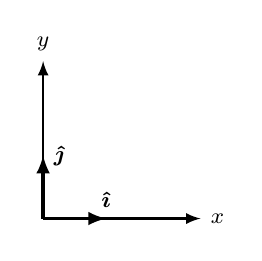
\begin{tikzpicture}
      \draw[axes] (0,0)--(2,0) node[right]{$x$};
      \draw[axes] (0,0)--(0,2) node[above]{$y$};
      \draw[vector] (0,0)--(.8,0) node[above]{$\iii$};
      \draw[vector] (0,0)--(0,.8) node[right]{$\jjj$};
    \end{tikzpicture}
    \caption{The 2D coordinate system is the $xy$-plane.}
  \end{subfigure}
  \begin{subfigure}{.3\linewidth}
    \centering
    \begin{tikzpicture}
      \draw[axes] (0,0)--(1.6,-.5) node[right]{$y$};
      \draw[axes] (0,0)--(-1,-.6) node[left]{$x$};
      \draw[axes] (0,0)--(0,1.7) node[above]{$z$};
    \end{tikzpicture}
    \caption{The 3D coordinate system is the Cartesian ($xyz$) space.}
  \end{subfigure}
  \caption{Cartesian coordinate systems}
  \label{fig:cartesian}
\end{figure}

\section{Kinematic Quantities}

\subsection{Position, Displacement and Distance}
Once the coordinate system has been established, we can describe where any
object is. \textbf{Position} is a vector describing the location of an object
in a coordinate system. In the IJK notation, position of an object is
expressed by its $x$, $y$ and $z$ components. If the object is in motion, then
the position vector is a function of time $t$.
\begin{equation*}
  \bm r(t)=
  \underbrace{x(t)\iii}_{\bm x(t)} +
  \underbrace{y(t)\jjj}_{\bm y(t)} +
  \underbrace{z(t)\kkk}_{\bm z(t)}
\end{equation*}
An example is shown in Fig.~\ref{fig:position}. The SI unit for position is a
\emph{metre} (\si{\metre}).
\begin{figure}[ht]
  \centering
  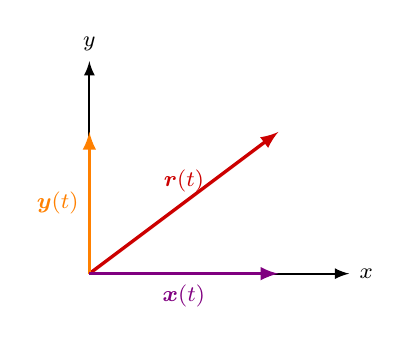
\begin{tikzpicture}[scale=.6]
    \draw[axes] (0,0)--(5.5,0) node[right]{$x$};
    \draw[axes] (0,0)--(0,4.5) node[above]{$y$};
    \draw[vector,red!80!black] (0,0)--(4,3) node[midway,above]{$\bm r(t)$};
    \draw[vector,orange] (0,0)--(0,3) node[midway,left]{$\bm y(t)$};
    \draw[vector,violet] (0,0)--(4,0) node[midway,below]{$\bm x(t)$};
    %    \draw[thick,dash dot,<->] (4,1)..controls (6,5) and (5,7)..(2,6)
    %    node[midway,right]{$s$};
  \end{tikzpicture}
  \caption{Position vector of an object inside a 2D cartesian coordinate
    system. The vectors $\bm x$ and $\bm y$ are the $x$ and $y$ components of
    $\bm r$ respestively.}
  %, displacement and distance in a Cartesian coordinate
  %  system.}
  \label{fig:position}
\end{figure}


When an object moves, the \textbf{displacement} is the change in position from
the initial position ($\bm r_o$) to the current position ($\bm r(t)$) within
the same coordinate system. Since the current position is a function of time,
so is displacement:
\begin{equation}
  \Delta\bm r(t)=\bm r(t)-\bm r_0
\end{equation}
A two-dimensional case is illustrated graphcin Fig.~\ref{fig:displacement}.
\begin{figure}[ht]
  \centering
  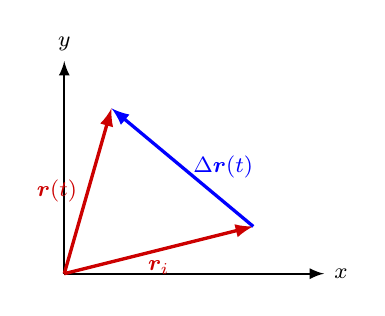
\begin{tikzpicture}[scale=.6]
    \draw[axes] (0,0)--(5.5,0) node[right]{$x$};
    \draw[axes] (0,0)--(0,4.5) node[above]{$y$};
    \draw[vector,red!80!black] (0,0)--(4,1) node[midway,below]{$\bm r_i$};
    \draw[vector,red!80!black] (0,0)--(1,3.5) node[midway,left]{$\bm r(t)$};
    \draw[vector,blue] (4,1)--(1,3.5) node[midway,right]{$\Delta \bm r(t)$};
  \end{tikzpicture}
  \caption{Displacement vector}
  \label{fig:displacement}
\end{figure}
In the cartesian coordinate system, the $x$, $y$ and $z$ axes are linearly
indepedent, displacement can be expressed by its components:
\begin{equation}
  \Delta\bm r(t)=%\Delta\bm r_x(t)-\bm r_i
  \underbrace{\left(x(t)-x_i\right)}_{\Delta r_x}\iii +
  \underbrace{\left(y(t)-y_i\right)}_{\Delta r_y}\jjj +
  \underbrace{\left(z(t)-z_i\right)}_{\Delta r_z}\kkk
\end{equation}
%The use of IJK notation makes vector addition and subtraction less prone to
%errors.
Like position, the SI unit for displacement is also a \emph{metre}. Note that
since ``reference point'' is the origin of the coordinate system, i.e.\
$\bm r_\text{ref}=\bm0$, any position vector $\bm r$ is also its displacement
from the reference point.


\textbf{Distance} $s$ is a quantity that is \emph{similar} (and related) to
displacement. It is the \emph{length of the path} taken when an object moves
from position $\bm r_o$ to current position $\bm r(t)$, as shown in
Fig.~\ref{fig:d-vs-d}. Unlike displacement, however, distance is a scalar
quantity that is always positive: $s\geq 0$, i.e.\ you can never walk a
\emph{negative} distance to the store. Because the path is not always a
straight line, therefore while the magnitude of the displacement vector is also
a scalar, it is not necessarily the same as distance:
\begin{equation}
  s(t)\geq |\Delta\bm r(t)|
\end{equation}



\subsection{Velocity and Speed}

\textbf{Velocity} is a quantity used to describe how \emph{fast} an object is
moving. If position $\bm r(t)$ is differentiable in time $t$, then its
\textbf{instantaneous velocity} $\bm v(t)$ can be found at any time $t$ by
differentiating $\bm r$ with respect to $t$. The SI unit for velocity is
\emph{meters per second} (\si{\metre\per\second}):
\begin{equation}
  \boxed{\bm v(t)= \diff{\bm r(t)}t}
\end{equation}
Since position $\bm r(t)$ has $x(t)$, $y(t)$ and $z(t)$ components along the
(linearly independent) $\iii$, $\jjj$ and $\kkk$ directions, we can take the
time derivative of every component to obtain the velocity components $v_x$,
$v_y$ and $v_z$ in those directions:
\begin{equation*}
  \bm v(t)= \diff{\bm r}t=
  \diff xt\iii + \diff yt\jjj + \diff zy\kkk =
  v_x\iii + v_y\jjj + v_z\kkk
\end{equation*}
By the fundamental theorem of calculus, if instantaneous velocity $\bm v(t)$
is the time derivative of position $\bm r(t)$ with respect to time $t$, then
$\bm r(t)$ is the time integral of $\bm v(t)$:
\begin{equation}
  \boxed{\bm r(t)=\int\bm v(t)\dl t + \bm r_0}
  \quad\text{or}\quad
  \boxed{\Delta\bm r(t)=\int_{t_0}^t\bm v(t)\dl t}
\end{equation}
The constant of integration $\bm r_0=\bm r(0)$ is the object's \emph{initial
position} at $t=0$. As was the case in differentiation, we can integrate each
component to get $\bm r$:
\begin{equation*}
  \bm r(t)= \left(
  \int v_x(t)\iii + \int v_y(t)\jjj + \int v_z(t)\kkk \right)\dl t + \bm r_0
\end{equation*}


The \textbf{average velocity} ($\overline{\bm v}$)\footnote{For
\emph{time averages}, the convention amongst \emph{most} physicists is to
write a bar over the quantity, as we have done here. In contrast, for
\emph{ensemble averages}, e.g.\ the average speeds of many particles, we use
the notation $\langle v\rangle$.} of an object is the change in position
$\Delta\bm r$ over a finite time interval $\Delta t$:
\begin{equation}
  \boxed{
    \overline{\bm v}(t)= \frac{\Delta\bm r}{\Delta t}
      =\frac{\int_{t_0}^t \bm r(t)dt}{t-t_0}
  }
\end{equation}
Like instantaneous velocity, we can find the $x$, $y$ and $z$ components of
average velocity by separating components in each direction:
\begin{equation*}
  \overline{\bm v}=
  \frac{\Delta x}{\Delta t}\iii +
  \frac{\Delta y}{\Delta t}\jjj +
  \frac{\Delta z}{\Delta t}\kkk =
  \overline v_x\iii +
  \overline v_y\jjj +
  \overline v_z\kkk
\end{equation*}



\textbf{Instantaneous speed} $v(t)$ is the rate of change of distance with
respect to time.\footnote{It is regrettable that both velocity and speed use
  the symbol $v$, but \emph{c'est la vie}.} Like velocity, the unit for
speed is also \si{\metre\per\second}:
\begin{equation*}
  \boxed{v(t)=\diff st}
\end{equation*}
Since distance is a scalar quantity, so too is speed. As distance along any
must be non-negative, i.e.\ $s(t)>0$, so must the instantaneous speed,
$v(t)\geq 0$. Instantaneous speed $v$ is the magnitude of the instantaneous
velocity vector $\bm v$. Likewise, \textbf{average speed} ($\overline v(t)$) is
similar to average velocity: it is the distance travelled over a finite time
interval.\footnote{It should be obvious that unlike instantaneous speed, average
  speed is not the magnitude of the average velocity.}
\begin{equation}
  \boxed{\overline v(t)=\frac s(t){\Delta t}}
\end{equation}


%\section{Path}
%
%Sometimes instead of explicitly describing the position $x=x(t)$ and $y=y(t)$,
%the path of an object can be given in terms of $x$ coordinate $y=y(x)$, while
%giving the $x$ (or $y$) coordinate as a function of time.
%\begin{itemize}
%\item In this case, substitute the expression for $x(t)$ into $y=y(x)$ to
%  get an expression of $y=y(t)$
%\item Take derivative using chain rule to get $v_y=v_y(t)$
%\end{itemize}


\subsection{Acceleration}

In the same way that velocity is the rate of change in position with respect
to time, \textbf{instantaneous acceleration} $\bm a(t)$ is the rate of change
in velocity with respect to time, and the second time derivative of position.
The SI unit for acceleration is \emph{meters per second squared}
(\si{\metre\per\second\squared}):
\begin{equation}
  \boxed{\bm a(t)= \diff{\bm v(t)}t=\diff[2]{\bm r(t)}t}
\end{equation}
%Although in grades 11 and 12 physics courses, students deal almost exclusively
%with constant ccceleration, in AP Physics, it must be understood that
%acceleration can also vary with time, and that calculus must be used in many
%cases.
%  \begin{enumerate}
%  \item Take derivative of $\bm x(t)$ to get $\bm v(t)=\bm x'(t)$
%  \item Take derivative again of $\bm v(t)$ to get $\bm a(t)=\bm v'(t)$
%  \end{enumerate}
%\end{frame}
Again, by the fundamental theorem of calculus, instantaneous velocity
$\bm v(t)$ is the time integral of instantaneous acceleration $\bm a(t)$:
\begin{equation}
  \boxed{\bm v(t)=\int\bm a(t)\dl t+\bm v_0} =
  \left(
  \int a_x\bm{\hat\imath} +
  \int a_y\bm{\hat\jmath} +
  \int a_z\bm{\hat k}
  \right)\dl t +\bm v_0
\end{equation}
where $\bm v_0$ is the initial velocity at $t=0$.

\subsection{Acceleration as Functions of Position and Velocity}

Since, according to the second law of motion, acceleration is proportional to
the net force ($F=ma$), therefore there are instances where acceleration is
often expressed as functions of other motion quantities rather than time. For
example:
\begin{itemize}[leftmargin=15pt]
\item\textbf{Gravitational force}\footnote{Newton's law of universal
  gravitation: $F_g=\dfrac{Gm_1m_2}{r^2}$} or
  \textbf{electrostatic force}\footnote{Coulomb's law:
    $F_q=\dfrac{kq_1q_2}{r^2}$} are both inversely proportional to
  the square of the distance (called the inverse-square law), and therefore
  acceleration is best express by this complicated differential equation:
  \begin{equation*}
    a(x)=\frac A{x^2} \quad\text{or}\quad \diff[2] xt=\frac A{x^2}
  \end{equation*}
  The solution will likely require numerical integration.

\item\textbf{Spring force} is proportional to displacement\footnote{By Hookes's
  law $\bm F_s=-k\bm x$, where $k$ is the spring constant that describes the
  stiffness of the spring}, and therefore acceleration is expressed as:
  \begin{equation*}
    a(x)=-bx\quad\text{or}\quad \diff[2] xt=-bx
  \end{equation*}
  The solution to this \emph{second-order ordinary differential equation with
    constant coefficient} is a sinusoidal function, i.e.\
  $x(t)=A\sin(\omega t+\phi)$, and the motion is a \emph{simple harmonic
    motion} that will be studied in a later topic.

\item\textbf{Damping force}  is usually proportional to velocity, leading
  to an expression for acceleration:
  \begin{equation*}
    a(v)=-cv\quad\text{or}\quad \diff vt=-cv
  \end{equation*}
  This time, the equation is a \emph{first-order ordinary differential equation}
  that can be solved by separating the $dt$ term and $v$ terms and then
  integrating, and the expression for velocity is an exponential function:
  \begin{equation*}
    \diff vt=-cv\quad\rightarrow\quad \int\frac{\dl v}{v}=-\int c\dl t
    \quad\rightarrow\quad \ln(v)=-ct+C
    \quad\rightarrow\quad v(t)=v_0e^{-ct}
  \end{equation*}
  Once the velocity expression is obtained, the expression for $x(t)$ and
  $a(t)$ can also easily be obtained by integrating and differentiating.

\item\textbf{Aerodynamic forces} such as drag and lift\footnote{The equations
  for lift and drag forces are $L=\dfrac12\rho v^2C_LA_\text{ref}$ and
  $D=\dfrac12\rho v^2C_DA_\text{ref}$ respectively, where $\rho$ is the density
  of the fluid, $A_\text{ref}$ is the reference area, $C_L$ is the lift
  coeffcient and $C_D$ is the drag coefficient}, which are proportional
  to the square of the velocity, leading to an expression for acceleration 
  \begin{equation*}
    a(v)=-kv^2\quad\text{or}\quad \diff vt=-kv^2
  \end{equation*}
  Not surprisingly, the process of solving the problem is similar to that of
  the damping function, but this time, the solution is a hyperbolic function:
  \begin{equation*}
    \diff vt=-kv^2\quad\rightarrow\quad \int\frac{\dl v}{v^2}=-\int k\dl t
    \quad\rightarrow\quad -\frac1v=-kt+C
    \quad\rightarrow\quad v(t)=\frac{1}{ct+C}
  \end{equation*}
\end{itemize}
In practice, multiple forces may act on an object, and each of them will be
functions of other motion quantities, and therefore the solution may require
solving more complex differential equations.

\subsection{Special Notation When Differentiating With Time}

Physicists and engineers often use a special notation when the derivative is
taken with respect to \emph{time} (and not spatial derivatives), by writing a
dot above the variable for \emph{first} derivative, and \emph{two} dots for
\emph{second} derivative, etc. For example, velocity is the first derivative
of position, i.e.\ $\bm v=\dot{\bm r}$ while acceleration is the second
derivative, i.e.\ $\bm a = \dot{\bm v}=\ddot{\bm r}$. This notation will be
used when it is convenient to do so.


\subsection{Higher Derivatives}

For anyone curious about higher derivatives, the time derivative of
acceleration is called \textbf{jerk} $\bm j(t)$ with a unit of
\si{\metre\per\second\cubed}:
\begin{equation}
  \bm j(t)=\diff{\bm a}t=\diff[2]{\bm v}t=\diff[3]{\bm r}t
\end{equation}
The measurement of jerk is used in many sensors, for example, in accelerometers
in airbags to determine if the acceleration of a car is under normal operation
(small $j$ value) or if a crash is in progress (high $j$ value). The time
derivative of jerk is \textbf{jounce}, or \textbf{snap}, with unit of
\si{\metre\per\second^4}:
\begin{equation}
  \bm s(t)=\diff{\bm j}t=\diff[2]{\bm a}t=\diff[3]{\bm v}t=\diff[4]{\bm r}t
\end{equation}
The next two derivatives of snap are called \textbf{crackle} and
\textbf{pop}\footnote{As in the cartoon mascots for Kellogg's rice crispies},
but these higher derivatives have little to know physical meaning, and are
therefore rarely used.



\subsection{Kinematic Equations for Constant Acceleration}

Although kinematic problems in AP Physics often require calculus\footnote{Unlike
  your AP Calculus exams, the differentiation/integration in AP Physics will be
  fairly straightforward}, basic kinematic equations for \emph{constant}
acceleration are still a very powerful tool. For constant acceleration
$\bm a$, velocity can be obtained by integrating in time:
\begin{equation}
  \bm v(t)=\int\bm a\dl t\quad\rightarrow\quad
  \boxed{\bm v(t)=\bm v_0+\bm at}
  \label{eq:big5-1}
\end{equation}
where $\bm v_0$ is the initial velocity at $t=0$. Integrating again for the
position vector:
\begin{equation}
  \bm r(t)=\int \bm v\dl t\quad\rightarrow\quad
  \boxed{\bm r(t)=\bm r_0+\bm v_0t+\frac12 \bm at^2}
  \label{eq:big5-2}
\end{equation}
where $\bm r_0$ is the initial position at $t=0$. The position vector is
quadratic in time.

The derivation of the last equation is slightly more laborious. From
Eqs.~\ref{eq:big5-1} and \ref{eq:big5-2}, if acceleration is constant, then
both the the velocity and position vectors are continuously differentiable. In
one-dimension\footnote{for simplicity}, the differentiation can be expressed as:
\begin{align*}
  \diff vt&=\diff vx\diff xt\\
  a&=v\diff vx
\end{align*}
Multiplying both sides by $\dl x$ and integrating, we have:
\begin{align*}
  \int_{x_0}^x a\dl x&=\int_{v_0}^v v\dl v\\
  a(x-x_0)&=\frac12\left(v^2-v_0^2\right)
\end{align*}
or in the more familiar form:
\begin{equation}
  \boxed{v^2 = v_0^2+ 2a(x-x_0)}
  \label{eq:big5-3}
\end{equation}
%Eqs.~\ref{eq:big5-1}, \ref{eq:big5-2} and \ref{eq:big5-3} are provided in the
%AP Exam equation sheet.


%  \textbf{One object:} the problem provides $3$ of the $5$ variables, and you
%  are asked to find a $4$th one.
%  \begin{itemize}
%  \item Define the positive direction (usually very obvious)
%  \item Apply the correct kinematic equation and solve the problem!
%  \end{itemize}
%
%  \vspace{.2in}\textbf{Two objects:} two objects are in motion. Usually one of
%  them is moving at constant velocity while the other is accelerating.
%  \begin{itemize}
%  \item Time interval $\Delta t$ and displacement $\Delta\bm x$ of the two
%    objects are related
%  \item Examples:
%    \begin{itemize}
%    \item Police car chasing a speeder
%    \item Two football players running towards each other
%    \item A person trying to catch the bus
%    \end{itemize}
%  \end{itemize}
%\end{frame}




%\section{One-Dimensional Motion Graphs for Constant Acceleration}

When analyzing one-dimensional motion, particularly experimental results, we
often use \textbf{motion graphs} to graphically express how motion quantities
(position, velocity, acceleration) evolves in time, or how they are related to
other motion quantities.

\section{Motion Quantities as Functions of Time}

The basic motion graphs most familiar to physics students in grades 11 and 12
are the graphs that express motion quantities as functions of time:
\begin{itemize}[nosep,leftmargin=15pt]
\item position vs.\ time (or displacement vs.\ time)
\item velocity vs.\ time
\item acceleration vs.\ time
\end{itemize}
Since velocity is the time derivative of position ($v=\dot{x}$), and
acceleration is the time derivative of velocity ($a=\dot{v}=\ddot{x}$), the
relationship between the graphs are straightforward: the velocity graph is the
slope of the position graph, and the acceleration graph is the slope of the
velocity graph.

\subsection{Areas Under a Graph}
The area under the acceleration vs.\ time graph is the change in velocity
$\Delta v$ and the area under the velocity vs.\ time graph to find displacement
$\Delta x$ based on the integral relationship:
\begin{align*}
 \Delta v&=\int a(t)dt\\
 \Delta x&=\int v(t)dt
\end{align*}
However, unless the functions $a(t)$ and $v(t)$ are known, or if the
graphs are simple, it is almost impossible to directly integrate. Instead,
numerical integration methods such as trapazoid rule or Simpson's rule are used
to approximate the area.



\subsection{Uniform Motion}

When an object moves along a straight line with \emph{constant} velocity
(i.e.\ both magnitude and direction of velocity are constant), the object's
motion is called \textbf{uniform motion}. The motion graphs for uniform
motion is shown in Fig.~\ref{fig:uniform-motion-graphs}. The position vs.\ time
graph for a uniform motion is a straight line, and its slope is the (constant)
velocity. Fig. 1.10a shows a uniform motion with a constant positive velocity.
Because velocity is constant, velocity vs.\ time graph is a horizontal straight
line, and the (constant) functional value of that graph is the (constant)
velocity of the object. An object in uniform motion has zero acceleration,
therefore the slope of the velocity versus time graph is 0, and the
acceleration versus time graph is a horizontal line that coincides with the
$x$-axis (time axis).
\begin{figure}[ht]
  \centering
  \begin{subfigure}{.3\textwidth}
    \centering
    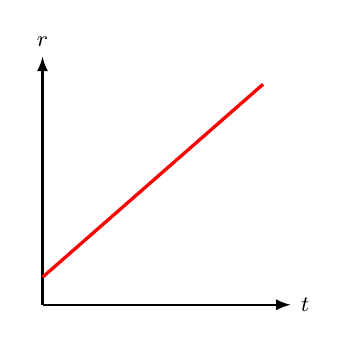
\begin{tikzpicture}[scale=.7]
      \draw[axes] (0,0)--(4.5,0) node[right]{$t$};
      \draw[axes] (0,0)--(0,4.5) node[above]{$r$};
      \draw[function] (0,.5)--(4,4);
    \end{tikzpicture}
    \caption{Position vs.\ time}
  \end{subfigure}
  \begin{subfigure}{.3\textwidth}
    \centering
    \begin{tikzpicture}[scale=.7]
      \draw[axes] (0,0)--(4.5,0) node[right]{$t$};
      \draw[axes] (0,0)--(0,4.5) node[above]{$v$};
      \draw[function] (0,2)--(4,2);
    \end{tikzpicture}
    \caption{Velocity vs.\ time}
  \end{subfigure}
  \begin{subfigure}{.3\textwidth}
    \centering
    \begin{tikzpicture}[scale=.7]
      \draw[axes] (0,0)--(4.5,0) node[right]{$t$};
      \draw[axes] (0,0)--(0,4.5) node[above]{$a$};
      \draw[function] (0,0)--(4,0);
    \end{tikzpicture}
    \caption{Acceleration vs.\ time}
  \end{subfigure}
  \caption{Basic motion graphs for uniform motion}
  \label{fig:uniform-motion-graphs}
\end{figure}


\subsection{Uniform Acceleration}

When a constant net force acts on an object, it moves with a constant
non-zero acceleration, or \textbf{uniform acceleration}. The position vs.\
time graph is a parabola, while velocity and acceleration graphs are linear, as
shown in Fig.~\ref{fig:uniform-acceleration-graphs}. Computing the area under
the velocity and acceleration graphs are straightforward, as is finding the
slope of the velocity graph, however, finding the acceleration using only the
position graph is much more difficult.
\begin{figure}[ht]
  \centering
  \begin{subfigure}{.3\textwidth}
    \centering
    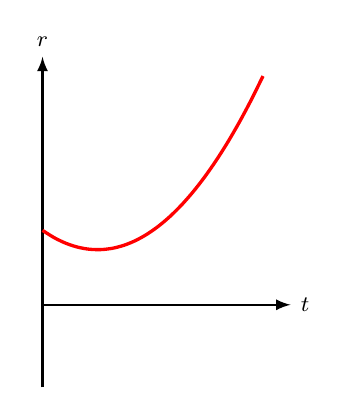
\begin{tikzpicture}[scale=.7]
      \draw[axes] (0,0)--(4.5,0) node[right]{$t$};
      \draw[axes] (0,-1.5)--(0,4.5) node[above]{$r$};
      \draw[function,samples=20,domain=0:4,smooth]
      plot(\x,{.35*(\x-1)*(\x-1)+1});
    \end{tikzpicture}
  \end{subfigure}
  \begin{subfigure}{.3\textwidth}
    \centering
    \begin{tikzpicture}[scale=.7]
      \draw[axes] (0,0)--(4.5,0) node[right]{$t$};
      \draw[axes] (0,-1.5)--(0,4.5) node[above]{$v$};
      \draw[function] (0,-1)--(4,2.5);
    \end{tikzpicture}
  \end{subfigure}
  \begin{subfigure}{.3\textwidth}
    \centering
    \begin{tikzpicture}[scale=.7]
      \draw[axes] (0,0)--(4.5,0) node[right]{$t$};
      \draw[axes] (0,-1.5)--(0,4.5) node[above]{$a$};
      \draw[function] (0,1)--(4,1);
    \end{tikzpicture}
  \end{subfigure}
  \caption{Motion graphs for uniformly accelerated motion}
  \label{fig:uniform-acceleration-graphs}
\end{figure}


\section{Advanced Graphing Techniques}

\subsection{Position vs. Time Squared}

In many cases, the position vs.\ time graph is often obtained by plotting
experimental values of $x$ and $t$. For example, photo gates can be used to
record the position of an object at regular time intervals. However, even if we
know that the acceleration is uniform, like the position vs.\ time graph
from Fig.~\ref{fig:uniform-acceleration-graphs}, it is still difficult to determine the
magnitude of acceleration\footnote{Of course, the \emph{sign} of the
  acceleration is easy to see, by looking at the concavity of the graph.} from
the graph. One way to get around this problem is to do a curve fitting.
However, curve fitting a parabola is time consuming. A much faster method is to
plot the motion quantities as a linear function instead.
%acceleration. Because the graph is obtained by joining discrete data points,
%and not from a function, you cannot simply ``take a derivative'' to find the
%velocity vs.\ time relationship.
%
%Instead, we can make an educated guess at what $a(t)$ \emph{should} look like
%(constant, exponential decay, oscillatory, etc), by a thorough analysis of all
%the forces acting on an object using a free-body diagram.
%and then making curve fit of the data, by making an educated guess that acceleration is
%uniform\footnote{This would have to be done
%and therefore the graph is a parabola.
%However, one of the weaknesses of this graph is the difficulty in determining
%the acceleration of the object by examining the graph itself. It is possible to
%take the second time derivative of the fitted curve to calculate the
%acceleration, which must be known algebraically in order to be plotted.
%Inevitably, some accuracy will be lost.

For example, if initial velocity is zero, ($v_0=0$), then instead of plotting
position $x$ directly against time $t$, we re-interpret the kinematic equation
as a linear function in the form of $y=mx+b$:
\begin{equation}
  \vertarrowbox{x}{$y$}=\vertarrowbox{\left(\frac12 a\right)}{$m$}
  \vertarrowbox{t^2}{$x$}+
  \cancel{v_0t}+
  \vertarrowbox{x_0}{$b$}
\end{equation}
and plot position $x$ against the \emph{square} of time, $t^2$. If acceleration
is indeed uniform, then the graph would be linear. That constant acceleration is
twice slope, i.e.:
\begin{equation*}
  m=\frac12 a\quad\rightarrow\quad a=2m
\end{equation*}
The $x$-intercept of both graphs are still the initial position $x_0$
(Fig.~\ref{switch1}). The $x$ vs.\ $t$ and the $x$ vs.\ $t^2$ graphs both
describe the same motion.
\begin{figure}[!ht]
  \centering
  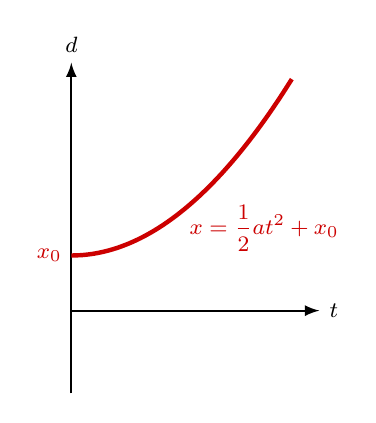
\begin{tikzpicture}[scale=.7]
    \draw[->,thick] (0,0)--(4.5,0) node[right]{$t$};
    \draw[->,thick] (0,-1.5)--(0,4.5) node[above]{$d$};
    \draw[smooth,samples=20,domain=0:4,red!80!black,ultra thick]
    plot({\x},{.2*(\x)*(\x)+1});
    \node[red!80!black] at (3.5,1.5) {$\displaystyle x=\frac12at^2+x_0$};
    \node[red!80!black] at (-.4,1) {$x_0$};
  \end{tikzpicture}
  \hspace{.15in}
  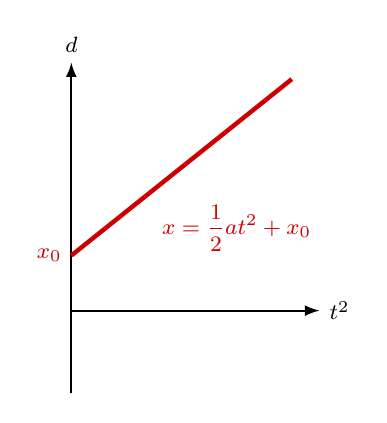
\begin{tikzpicture}[scale=.7]
    \draw[axes] (0,0)--(4.5,0) node[right]{$t^2$};
    \draw[axes] (0,-1.5)--(0,4.5) node[above]{$d$};
    \draw[red!80!black,ultra thick](0,1)--(4,4.2);
    \node[red!80!black] at (3,1.5) {$\displaystyle x=\frac12at^2+x_0$};
    \node[red!80!black] at (-.4,1) {$x_0$};
  \end{tikzpicture}
  \caption{Position plotted against time $t$ and time squared $t^2$ for
    uniformly accelerated motion.}
  \label{switch1}
\end{figure} 


\subsection{Velocity Squared vs.\ Displacement}
Likewise, some experimental equation is able to capture velocity information
as an object moves in \emph{space}. In other words, velocity and position
information is available experimentally but not time. Instead of plotting
velocity vs.\ time, position vs.\ time, we can plot velocity as a function of
\emph{position}. Again, even if acceleration is uniform, finding $a$ from this
graph is not straightforward. However, another option is to, like in the
previous section, re-interpret the kinematic equation as a linear function:
\begin{equation}
  \vertarrowbox{v^2}{$y$}=
  \vertarrowbox{v_0^2}{$b$}+\vertarrowbox{(2a)}{$m$}
  \vertarrowbox{(x-x_0)}{$x$}
\end{equation}
and plot the \emph{square} of velocity $v^2$ as a function of
displacement ($x-x_0$). If acceleration is uniform (constant $a$), the graph
would be linear. The acceleration is half the slope $m$ of the graph:
$a=\dfrac m2$ and the $y$-intercept is the square of the initial velocity
($v_0^2$).


%\subsection{Use of Linear Graphs in Other Applications}
%There are many types of graphs that we plot as linear graphs even though the
%relationship between variables is not linear. In the AP Physics C exams, there
%is often one free-response question where ``experimental'' data is provided for
%a known algebraic relationship, and you as asked to find a constant by plotting
%a linear graph. Some example are shown here.


\subsection{Orbital Mechanics}
The relationship between the period $T$ and orbital radius $R$ of planets
around the same star (Kepler's third law of planetary motion) is most often
shown by plotting $T^2$ vs.\ $R^3$ rather than plotting $T$ vs.\ $R$ directly.
The slope of the graph can be used to find the mass of the star $M$
at the center:
\begin{equation}
  \vertarrowbox{T^2}{$y$}=
  \vertarrowbox{\dfrac{4\pi^2}{GM}}{$m$}
  \vertarrowbox{R^3}{$x$}
\end{equation}



\subsection{Simple Pendulum}
In the simple harmonic motion of a simple pendulum, the relationship between
the frequency $f$ and the length of the pendulum $\ell$ is given
by\footnote{Although \emph{usually} we would write it as
  \begin{equation*}
    f=\frac1{2\pi}\sqrt{\frac \ell{g}}
  \end{equation*}
}
\begin{equation}
  f=\left[\frac1{2\pi\sqrt{g}}\right]\sqrt{\ell}
\end{equation}
In this case, the slope of the graph of $f$ vs.\ $\sqrt\ell$ can be used to
experimentally determine the acceleration due to gravity $g$.



\subsection{Refraction of Light}
In the law of refraction\footnote{You may know it as Snell's law.}, the
incident angle $\theta_1$ and the refracted angle $\theta_2$ when light is
refracted from a vaccuum into a material with refractive index $n$ is given
by:
\begin{equation}
  \vertarrowbox{\sin\theta_1}{$y$}=
  \vertarrowbox{n}{$m$}
  \vertarrowbox{\sin\theta_2}{$x$}
\end{equation}
By plotting $\sin\theta_1$ vs.\ $\sin\theta_2$, we see that the slope of the
graph is the refractive index.

%\section{Projectile Motion}
A \textbf{projectile} is an object that is launched with an initial velocity
of $\bm V_0$ at an angle $\theta$ with the horizontal. It travels along a
parabolic trajectory and accelerates only due to gravity, as shown in
Figure~\ref{fig:projectile}. 
\begin{figure}[ht]
  \centering
  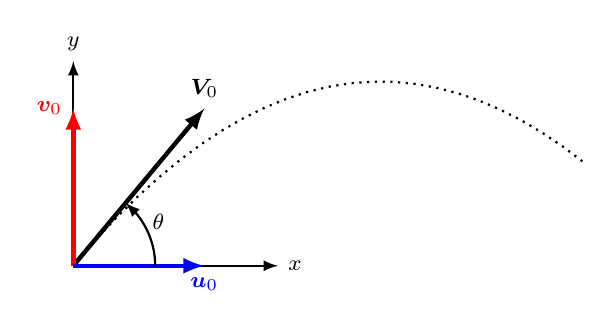
\begin{tikzpicture}[scale=1.3]
    \draw[thick,->](0,0)--(2,0) node[right]{$x$};
    \draw[thick,->](0,0)--(0,2) node[above]{$y$};
    \draw[dotted,domain=0:5,thick] plot (\x, {1.2*\x-.2*\x*\x});
    \begin{scope}[ultra thick,->]
      \draw[rotate=atan(1.2)](0,0)--(2,0)node[above]{$\bm V_0$};
      \draw[red] (0,0)--(0,2*sin{atan{1.2}}) node[left]{$\bm v_0$};
      \draw[blue](0,0)--(2*cos{atan{1.2}},0)node[below]{$\bm u_0$};
    \end{scope}
    \draw[thick,->](.8,0)arc(0:atan{1.2}:.8) node[pos=.65,right]{$\theta$};
  \end{tikzpicture}
  \caption{The parameters defining the motion of a projectile.}
  \label{fig:projectile}
\end{figure}

In general, when solving a projectile motion project:
\begin{itemize}[nosep]
\item the $x$-axis ($\iii$ direction) is defined as the \emph{horizontal}
  direction, with the ($+$) direction pointing forward
\item the $y$-axis ($\jjj$ direction) is the \emph{vertical} direction, with
  the ($+$) direction pointing upwards
\item the origin of the coordinate system is where the projectile is launched
\item the launch angle is ($+$) if it is above the horizontal, and ($-$) if it
  is below
\end{itemize}
This set up is consistent with the standard right-handed Cartesian coordinate
system. The initial velocity $\bm V_0$ can be resolved into its $\iii$ and
$\jjj$ components, $\bm u_0$ and $\bm v_0$:
\begin{equation}
  \bm V_0 =\bm u_0+\bm v_0
  =\left[V_0\cos\theta\right]\iii + \left[V_0\sin\theta\right]\jjj
\end{equation}
where $V_0=|\bm V_0|$.

\subsection{Motion in the Horizontal Direction}
There is no acceleration (i.e.\ $a_x=0$) along the $\iii$ direction, therefore
horizontal velocity is a constant $u=u_0$. The kinematic equations are reduce
to a single equation that relates the horizontal position (displacement) $x$ as
a function of time:
\begin{equation}
  x(t)=u_0t=\left[V_0\cos\theta\right] t
  \label{eq:x}
\end{equation}

\subsection{Motion in the Vertical Direction}
There is a constant acceleration due to gravity alone along the $\jjj$
direction, i.e.\ $a_y=-g$. (Acceleration is \emph{negative} due to the fact that
the positive $y$-axis points upwards.) The kinematic equations along the
vertical direction are therefore:
\begin{align}
  y(t) &= \left[V_0\sin\theta\right]t-\frac12gt^2\label{eq:y}\\
  v(t) &= \left[V_0\sin\theta\right] -gt\\
  \left[v(y)\right]^2&=V_0^2\sin^2\theta-2gy
  \label{eq:maxh}
\end{align}

\subsection{Solving Projectile Motion Problem}
For most projectile motion problems, Eqs.~\ref{eq:x} and \ref{eq:y} are the
most often used. Because $\iii$ and $\jjj$ directions are orthogonal, and
therefore \emph{linearly independent}, horizontal and vertical displacements
$x(t)$ and $y(t)$ are independent of each other. However, there are also
variables that are shared in both directions, namely:
\begin{itemize}[nosep,leftmargin=12pt]
\item Time $t$
\item Launch angle $\theta$
\item Initial speed $V_0$
\end{itemize}
When solving for most projectile motion problems, there likely will be two
unknowns that need to be solved (although you may not be explicitly told what
one of them is), requiring two equations (the $x$ and $y$ kinematic equations).
In some rare cases, if an object lands on an incline, there will be a third
equation describing the relationship between $x$ and $y$ of the incline.

\subsection{Parabolic Path}
We can easily see that the path of a projectile is entirely parabolic. When
solving for the flight time in the $x$ direction (Eq.~\ref{eq:x}), we get:
\begin{equation}
  t=\frac x{V_0\cos\theta}
  \label{eq:t1}
\end{equation}
Substituting Eq.~\ref{eq:t1} into Eq.~\ref{eq:y}, we have
\begin{align}
  y &=\left(V_0\sin\theta\right) t-\frac12gt^2\nonumber\\
  &= \left(V_0\sin\theta\right)\left(\frac x{V_0\cos\theta}\right)-\frac12g
  \left(\frac x{V_0\cos\theta}\right)^2\nonumber\\
  y&=\left(\tan\theta\right) x-\left(\frac g{2V_0^2\cos^2\theta}\right)x^2
\end{align}
It is clear that the $y$ is quadratic in $x$, and therefore the path is a
parabola in space.

\subsection{Symmetric Projectiles}
A projectile's trajectory is \emph{symmetric} where an object is launched an
angle of $\theta$ (between \ang{0} and \ang{90}) above the
horizontal%\footnote{This may be obvious, but angles \emph{below} the
%horizontal will never have a symmetric trajectory.} and then
lands at the same height. Examples may include hitting a golf ball towards the
hole, or shooting a bullet toward a horizontal target\footnote{Shooting a
bullet toward a horizontal target always require an upward angle because of
gravity.}
%\footnote{Note that the equations for symmetric trajectory are \emph{not}
%  included in the AP Exam equation sheet; if you need these equations during
%sma  the exams, you will need to derive them yourself. Thankfully, the derivation
%  is striaghtforward.}

Applying the kinematic equation first in the $\jjj$ direction. When the object
lands at the same height at time $T$, the final displacement is $y(T)=0$:
\begin{equation*}
  y(T)=V_0\sin\theta T-\frac12gT^2=0
\end{equation*}
Solving for $T$ we find the \textbf{total time of flight}:
\begin{equation}
  \boxed{
    T=\frac{2V_0\sin\theta}g
  }
  \label{tmax}
\end{equation}
Not surprisingly, a projectile will stay in the air the longest when it is
launched at $\theta=\ang{90}$.
%\footnote{As a fun exercise, for a known initial
%  speed $V_0$, you can plot $t$ vs.\ $\sin\theta$ to find the acceleration due
%  to gravity $g$!}
Mathematically, there is a second (trivial\footnote{Trivial means
\emph{unimportant}}) solution, at $T=0$. Of course, it just means that the
project has zero vertical displacement at the moment when it is launched.

Next, we apply the kinematic equation (Eq.~\ref{eq:maxh}) in the $\jjj$
direction. Recognizing that at maximum height $y=H$, the vertical component of
velocity is zero $v(H)=0$:
\begin{equation*}
  v^2 = V_0^2\sin^2\theta-2gH = 0
\end{equation*}
Solving for $H$, we get the equation for \textbf{maximum height}:
\begin{equation}
  \boxed{H=\frac{V_0^2\sin^2\theta}{2g}}
\end{equation}
The maximum height also (not surprisingly) has a maximum value when
$\theta=\ang{90}$.

Finall, we substitute the expression for total time of flight $T$ from
Eq.~\ref{tmax} into the $t$ term, then apply the kinematic equation in the
$\iii$ irection to compute the \textbf{range} $R=x(T)$ for any given launch
angle and initial speed:
\begin{equation}
  R=x(T)=u_0T=V_0\cos\theta\left[\frac{2V_0\sin\theta}g\right]
  \label{step1}
\end{equation}
Using the trigonometric identity $\sin(2\theta)=2\sin\theta\cos\theta$,
Eq.~\ref{step1} simplifies to:
\begin{equation}
  \boxed{R=\frac{V_0^2\sin(2\theta)}g}
\end{equation}
It is obvious that for any given initial speed $V_0$, the maximum range
$R_\text{max}$ occurs at an angle where $\sin(2\theta)=1$ (i.e.\
$\theta=\ang{45}$), with a value of
\begin{equation}
  \boxed{R_\text{max}=\frac{V_0^2}g}
\end{equation}
Also, for a known initial speed $V_0$ and range $R$ we can compute the launch
angle $\theta$:
\begin{displaymath}
  \theta_1=\frac12\sin^{-1}\left(\frac{gR}{V_0^2}\right)
\end{displaymath}
This angle is labelled $\theta_1$ because it is \emph{not} the only angle that
can reach this range. Recall that for any angle $0<\phi_1<\ang{180}$, there
is also another angle $\phi_2=\ang{180}-\phi_1$ where sine of the angles has the
same value:
\begin{displaymath}
  \sin\phi=\sin(\ang{180}-\phi)
\end{displaymath}
Which means that for any $\theta_1$, there is also another angle $\theta_2$
where $2\theta_2=\ang{180}-2\theta_1$, or simply:
\begin{equation}
  \boxed{
    \theta_1+\theta_2=\ang{90}
  }
\end{equation}

%
%\chapter{Dynamics of Rigid Bodies}
\label{chapter:dynamics}

While \textbf{kinematics} describes the motion of any object mathematically,
\textbf{dynamics} describes \emph{what} causes motion to change


\section{Forces}


\section{Laws of Motion}

The first law of motion, as stated in \emph{Principia}, says that:
\begin{center}
  \fcolorbox{black}{cyan!10}{
    \begin{minipage}{.74\textwidth}
      \textbf{Law \#1: An object will remain in its state of rest or uniform
        motion, until a net external force is applied to it.}\footnote{Lex I:
      Corpus omne perseverare in statu suo quiescendi vel movendi uniformiter
      in directum, nisi quatenus a viribus impressis cogitur statum illum
      mutare.}
    \end{minipage}
  }
\end{center}
This called, called the \emph{law of equilibrium}, states that when the sum
of all the forces acting on an object is balanced, the velocity of the object
will not change.

When the net force on an object is zero ($\sum\bm F=\bm 0$) then the
object is in a \emph{state of translational equilibrium}. Equilibrium can be
either:
\begin{itemize}[nosep,leftmargin=12pt]
\item\textbf{dynamic equilibrium} when the object is moving relative to the
  observer), or
\item\textbf{static equilibrium}, when the object is not moving relative to the
  observer
\end{itemize}
%\begin{itemize}
%\item Uniform motion means constant velocity; an object ``at rest'' is also
%  in uniform motion with $\bm v=\bm 0$
%\item As long as an object moves in uniform motion, it must be that
%  
%\item Common examples:
%  \begin{itemize}
%  \item A hockey puck sliding on very smooth ice has gravity and normal
%    force, but the net force is zero
%  \item A car traveling on a highway at \SI{100}{\kilo\metre\per\hour}
%    has many forces acting on it, but the net force is zero 
%  \end{itemize}
%\item{\color{red!80!black}This is a special case that assumes a constant
%  mass}
%\end{itemize}

%\subsubsection{Aristotle: The Wrong Interpretation}
Prior to Galileo, the understanding of motion came primarily from Greek
philosopher Aristotle, who said that any body in motion will come its
natural state: at rest. Aristotle's idea ``makes sense'' from everyday
experience. For example: slide a book across a table, it will eventually stop.
However, Galileo pointed out that Aristotle's philosophy is ambiguous: absolute
rest cannot be determined because all motion is relative.

\textbf{Absolute rest cannot be determined:} Objects that are stationary in one
coordinate system can be moving relative to another (see \emph{relative motion}
from last class). A cup of water, shown in Fig.~\ref{fig:cup}, is on the tray
table on an airplane in flight. The cup is stationary relative to the
passengers, but moving relative to anyone outside watching the airplane fly by.
\begin{figure}[ht]
  \centering
  \pic{.4}{../dynamics-calculus/coffeecup}
  \caption{A cup of water on an airplane is flight is stationary only
    passengers on the airplane, but not to observers outside}
  \label{fig:cup}
\end{figure}

\textbf{Uniform motion is indistinguishable from rest:} If I drop a tennis ball
while standing on the ground (Fig~\ref{fig:tennisball}), the ball falls
straight down with an acceleration due to gravity. If I repeat this while on an
airplane travelling in uniform motion (i.e.\ constant velocity) in the air, I
will observe exactly the same thing. The motion of the ball gives me no
information about whether I am at rest on in uniform motion
\begin{figure}[ht]
  \centering
  \pic{.4}{../dynamics-calculus/Aging-Self-2}
  \caption{Observing the motion of a dropped tennis ball gives no hint as to
    whether you are stationary or moving in uniform motion.}
  \label{fig:tennisball}
\end{figure}
  
\begin{center}
  \fcolorbox{black}{cyan!10}{
    \begin{minipage}{.7\textwidth}
      \textbf{Law \#2: The acceleration of an object is proportional to,
        and along the direction of, the net external force.}\footnote{Lex II:
      Mutationem motus proportionalem esse vi motrici impressae, et fieri
      secundum lineam rectam qua vis illa imprimitur.}
    \end{minipage}
  }
\end{center}

Like the first law, the second law of motion as descrribed by Newton is also a
``special case'' that assumes a constant mass. We can summarize the first two
laws into one of the most recognizable equation:
\begin{equation}
  \boxed{
    \bm F_\text{net}(t)=\sum\bm F=m\bm a(t)
  }
\end{equation}

For non-constant mass, net force is the rate of change of momentum $\bm p$.
\begin{equation*}
  \bm F_\text{net}(t)=\diff{\bm p}t
\end{equation*}
The topic of momentum will be studied in more depth in
Chapter~\ref{chapter:momentum}.


\subsection{Defining Mass}
What is \textbf{mass} then? It is
\begin{itemize}
\item the property of an object that relates its acceleration to the force
  applied to it. Literally, it means:
  \begin{equation}
    m\equiv\frac{F_\text{net}}a
  \end{equation}
\item Intrinsic to the object itself
\item This is explicitly referred to as the object's \textbf{inertial mass}
\end{itemize}




\section{Third Law of Motion}
\begin{center}
  \fbox{
    \begin{minipage}{.9\textwidth}
      \textbf{Law \#3: For every action there is always an opposite and
        equal reaction; the mutual actions of two objects on each other are
        always equal, and directed to the other object.}
    \end{minipage}
  }
\end{center}

Whenever object (B) exerts any force on object (A), (A) will immediately
exert a reaction force on (B) that is equal in magnitude but opposite in
direction:
\begin{equation}
  \boxed{\bm F_\text{AB} = -\bm F_\text{BA}}
\end{equation}
\begin{itemize}
\item The action and reaction forces act on different objects!
\item Third law is an application of the first law. Action/reaction forces
  are \emph{internal} forces to the system of objects.
\end{itemize}



\section{Forces}
A \textbf{force} is the interaction between the objects.
\begin{itemize}
\item When there is interaction, then forces are created
\item A ``push'' or a ``pull''
\end{itemize}
There are two broad categories of forces:
\begin{itemize}
\item\textbf{Contact forces} act between two objects that are in contact
  with one another
\item\textbf{Non-contact forces} act between two objects without them
  touching each other. They are also called ``action-at-a-distance'' force
\end{itemize}


Common forces that we encounter may include:
\begin{itemize}[nosep,leftmargin=12pt]
\item Weight (gravitational force) $\bm F_g$
\item Normal force $\bm F_N$
\item Friction force (static $\bm f_s$ and kinetic $\bm f_k$)
\item Tension force $\bm F_T$
\item Applied force $\bm F_a$
\item Spring force $\bm F_s$
\item Aerdynamic drag $\bm F_D$ (a.k.a.\ fluid resistance)
\item Buoyant force $\bm F_B$ (discussed in fluid mechanics, in AP Physics 2)
\item Electrostatic force $\bm F_q$ (discussed in E \& M)
\item Magnetic force $\bm F_m$ (discussed E \& M)
\end{itemize}




\subsection{Gravity}
Gravity is the force of attraction between all objects with mass
\begin{equation}
  \boxed{\bm F_g=m\bm g}
\end{equation}
\begin{itemize}
\item Near surface of Earth, use $g=\SI{9.81}{\metre\per\second\squared}$ (or
  $g=\SI{10}{\metre\per\second\squared}$ for your AP exam)
\item $\bm F_g$ always points \emph{down}
\item Based on the law of universal gravitation:
  \begin{equation*}
    \boxed{F_g=\frac{Gm_1m_2}{r^2}}\;\;
    \text{\normalsize where}\;\;
    G=\SI{6.674e-11}{\newton\metre\squared\per\kilo\gram\squared}
  \end{equation*}
\end{itemize}  




\subsection{Normal Force}
\begin{figure}[ht]
  \centering
  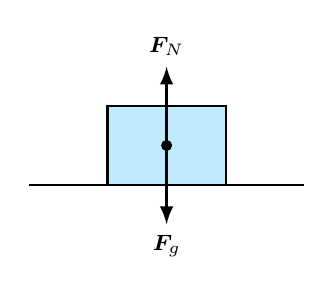
\begin{tikzpicture}
    \draw[thick] (-1,0)--(2.5,0);
    \draw[mass] rectangle (1.5,1);
    \fill (.75,.5) circle (2pt);
    \draw[vector] (.75,.5)--(.75,-.5) node[below]{$\bm F_g$};
    \draw[vector] (.75,.5)--(.75,1.5) node[above]{$\bm F_N$};
  \end{tikzpicture}
    %$\bm F_g=-\bm F_N$\\(special case)
\end{figure}

\begin{itemize}
\item A force a surface exerts on another object that it is in contact with
\item Always \textbf{perpendicular} to the contact surface
\item\textbf{Special case:} When an object is on a horizontal surface
  with no additional applied force, the magnitude of the normal force is
  equal to the magnitude of the weight of the object, i.e.\ $N=mg$
\end{itemize}

The normal force remains perpendicular to the support surface even when it is
at an angle:
\begin{figure}[ht]
  \centering
  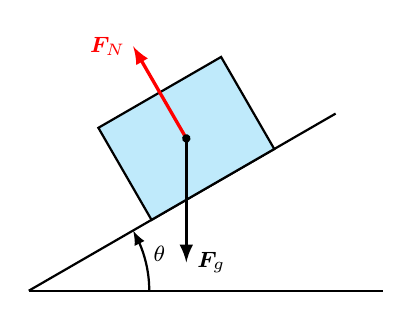
\begin{tikzpicture}[scale=.9]
    \draw[thick] (0,0)--(5,0);
    \draw[axes] (1.7,0) arc (0:30:1.7) node[pos=.6,right] {$\theta$};
    \begin{scope}[rotate=30]
      \draw[thick] (0,0)--(5,0);
      \draw[mass] (2,0) rectangle (4,1.5);
      \draw[vector,rotate around={-30:(3,.75)}]
      (3,.75)--(3,-1) node[right]{$\bm F_g$};
      \draw[vector,red] (3,.75)--(3,2.25) node[left=-1]{$\bm F_N$};
      \fill (3,.75) circle (.06);
    \end{scope}
  \end{tikzpicture}
\end{figure}
\textbf{Important note:} It is not always clear what the magnitude of the
normal force is. Finding the magnitude of the normal force is part of the
analysis process.




%%\begin{frame}{Normal Force on a Stationary Slope}
%  For this case, we define the $x$-axis to be along the slope, and $y$-axis to
%  be perpendicular to the slope.
%  \begin{columns}
%    \column{.35\textwidth}
%    \centering
%    \begin{tikzpicture}[scale=.9]
%      \draw[thick] (-1,0)--(3,0);
%      \draw[thick,->](.1,0) arc(0:37:1.1) node[pos=0,below]{$\theta$};
%      \begin{scope}[rotate around={37:(-1,0)}]
%        \draw[->](3.5,.5)--(4,.5)  node[right]{$x$};
%        \draw[->](3.5,.5)--(3.5,1) node[above]{$y$};
%        \draw[thick] (-1,0)--(4,0);
%        \draw[fill=cyan!80,thick] rectangle (3,2);
%        \fill(1.5,1) circle (2pt);
%        \draw [->,very thick,dotted,red] (1.5,1)--(1.5,-.5)
%        node[right]{$mg\cos\theta$};
%        \draw [->,very thick,dotted,red] (1.5,1)--(.45,1)
%        node[left]{$mg\sin\theta$};
%        \draw [->,very thick,red] (1.5,1)--(.45,-.5)
%        node[below]{$\bm F_g$};
%        \draw [->,very thick] (1.5,1)--(1.5,2.5) node[above]{$\bm F_N$};
%      \end{scope}
%    \end{tikzpicture}
%    
%    \column{.65\textwidth}
%    \begin{itemize}
%    \item On a stationary slope: $N=mg\cos\theta$
%      \begin{itemize}
%      \item $N$ decreases as ramp angle $\theta$ increases
%      \end{itemize}
%    \item Weight has a component along the ramp ($mg\sin\theta$) that wants
%      to slide the block down.
%    \end{itemize}
%  
%



\subsection{Friction}
\begin{itemize}
\item A force that opposes the sliding of two surface against one another
\item Always act in a direction that opposes motion or attempted motion
\item Depends on:
  \begin{itemize}
  \item Normal force $N$: The force the two surfaces are pressed against
    each other
  \item Coefficients of friction ($\mu_s$ and $\mu_k$): Smoothness of the
    surfaces, which itself depends on
    \begin{itemize}
    \item The material(s) the surfaces are made of
    \item The use of lubricants
    \end{itemize}
  \end{itemize}
\end{itemize}
\begin{center}
  \pic{.5}{../dynamics-calculus/graphics/friction}
\end{center}




\subsubsection{Static Friction}
When there is no relative motion between the two surface, the friction is
called the \textbf{static friction}
%  \textbf{Static friction} between the two surfaces is when there is no
%  relative motion between them
\begin{itemize}
\item Increases with increasing applied force
\item Maximum when the object is just about to move
\end{itemize}
\begin{equation}
  \boxed{f_s\leq\mu_sN}
\end{equation}
\begin{center}
  \begin{tabular}{l|c|c}
    \rowcolor{pink}
    \textbf{Quantity} & \textbf{Symbol} & \textbf{SI Unit} \\ \hline
    Magnitude of static friction & $f_s$ & \si\newton \\
    Coefficient of static friction & $\mu_s$ & no units \\
    Magnitude of normal force    & $N$ & \si\newton
  \end{tabular}
\end{center}




\subsubsection{Kinetic Friction}
When the two surfaces are moving relative to each other, the friction is
called \textbf{kinetic friction} $f_k$. $f_k$ is approximately constant along
the path of movement as long  as $\bm F_N$ stays constant
\begin{equation}
  \boxed{f_k = \mu_kN}
\end{equation}
\begin{center}
  \begin{tabular}{l|c|c}
    \rowcolor{pink}
    \textbf{Quantity} & \textbf{Symbol} & \textbf{SI Unit} \\ \hline
    Magnitude of kinetic friction & $f_k$ & \si\newton \\
    Coefficient of kinetic friction & $\mu_k$ & no units \\
    Magnitude of normal force & $N$ & \si\newton
  \end{tabular}
\end{center}




%\begin{frame}{Static and Kinetic Coefficients of Friction}    
Coefficient of kinetic friction is always lower than the coefficient for
static friction, otherwise nothing will ever move:
\begin{equation}
  \mu_k\leq\mu_s
\end{equation}

Consider a simple case of a box being pulled along a level floor. The free-body
diagram is simple (left). How do the magnitudes of the applied force $F_a$ and
friction $f$ compare?

\begin{figure}[ht]
  \centering
  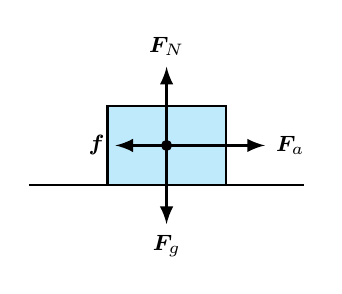
\begin{tikzpicture}
    \draw[thick] (-1,0)--(2.5,0);
    \draw[mass] rectangle (1.5,1);
    \fill (.75,.5) circle (2pt);
    \draw[vector] (.75,.5)--(.75,-.5) node[below]{$\bm F_g$};
    \draw[vector] (.75,.5)--(.75,1.5) node[above]{$\bm F_N$};
    \draw[vector] (.75,.5)--(2.,.5) node[right]{$\bm F_a$};
    \draw[vector] (.75,.5)--(.1,.5) node[left]{$\bm f$};
  \end{tikzpicture}
\end{figure}
%    \column{.6\textwidth}
%    \centering
%    \begin{tikzpicture}[scale=.5,vector]
%      \draw (0,0)--(10,0) node[right]{$F_a$};
%      \draw (0,0)--(0,5) node[left]{$f$};
%    \end{tikzpicture}
  




%\begin{frame}{Tires}
Most people associate friction as the force that slows down things, but very
often friction is what accelerates things. \textbf{Example:} the forward
acceleration of a car is caused by the static friction between the tires and
the road.
\begin{center}
  \pic{.38}{../dynamics-calculus/graphics/all-season-tires}
\end{center}
Tires also generated a force called \emph{rolling resistance} as it rolls
along a road because the weight of the car deforms the tires.





\subsection{Drag}
\label{sec:drag}
When an object moves through a fluid (most gases and liquids), it experiences
a fluid resistance force called \textbf{drag} $\bm F_D$. It is defined as:
\begin{equation}
  \boxed{
    F_D=\frac12\rho v_\infty^2C_DA
  }
\end{equation}
Unlike kinetic friction, drag force scales with the square of the speed of the
object relative to the fluid that it is moving in:
\begin{figure}[ht]
  \pic{.338}{../dynamics-calculus/graphics/boeing787}
  \pic{.35}{../dynamics-calculus/graphics/ganna}
  \pic{.263}{../dynamics-calculus/graphics/submarine}
  \caption{Object moving through fluids will experience a drag force}
  \label{fig:drag}
\end{figure}
At this time, you are not required to know the drag equation, just that
$F_D\propto v^2$, and $F_D\propto A$
%\begin{equation}
%  \boxed{
%    F_D=\frac12\rho v_\infty^2C_DA
%  }
%\end{equation}  
%\begin{center}
%  \begin{tabular}{l|c|c}
%    \rowcolor{pink}
%    \textbf{Quantity} & \textbf{Symbol} & \textbf{SI Unit} \\ \hline
%    Magnitude of drag force & $F_D$     & \si\newton \\
%    Density of the fluid    & $\rho$    & \si{\kilo\gram\per\metre\cubed}\\
%    Free-stream velocity    & $v_\infty$ & \si{\metre\per\second}\\
%    Reference area          & $A$       & \si{\metre\squared}\\
%    Drag coefficient        & $C_D$     & (no unit)
%  \end{tabular}
%\end{center}
Drag force also depends on the \textbf{drag coefficient} $C_D$,
a non-dimensional variable that depends on the shape and surface smoothness of
the object.
For blunt objects (``bluff bodies'') $A$ is the frontal area; for
streamlined objects $A$ is the planform (top-view) area.

When we take drag force into account, we understand that the drag force
increases as an object speeds up, and therefore a free-falling object does
\emph{not} accelerate infinitely. Instead it reaches a
\textbf{terminal velocity}.

\begin{figure}[ht]
  \centering
  \begin{subfigure}{.31\textwidth}
    \centering
    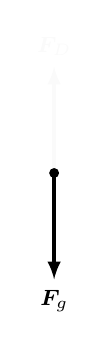
\begin{tikzpicture}[scale=.9,vector]
      \draw (0,0)--(0,-1.5) node[below]{$\bm F_g$};
      \draw[black!2] (0,0)--(0,1.5) node[above]{$\bm F_D$};
      \fill circle (.07);
    \end{tikzpicture}    
    \caption{There is no air resistance just as the object \emph{begins}
      to fall. Acceleration is due to gravity alone.}
  \end{subfigure}
  \begin{subfigure}{.31\textwidth}
    \centering
    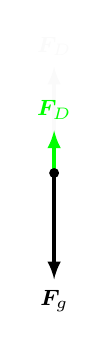
\begin{tikzpicture}[scale=.9,vector]
      \draw (0,0)--(0,-1.5) node[below]{$\bm F_g$};
      \draw[black!2] (0,0)--(0,1.5) node[above]{$\bm F_D$};
      \draw[green] (0,0)--(0,.6) node[above]{$\bm F_D$};
      \fill circle (.07);
    \end{tikzpicture}
    \caption{Drag increases as $v$ increases. Magnitude of acceleration
      decreases, but the object continues to gather speed}
  \end{subfigure}
  \begin{subfigure}{.31\textwidth}
    \centering
    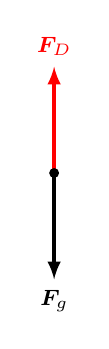
\begin{tikzpicture}[scale=.9,vector]
      \draw (0,0)--(0,-1.5) node[below]{$\bm F_g$};
      \draw[red] (0,0)--(0,1.5) node[above]{$\bm F_D$};
      \fill circle (.07);
    \end{tikzpicture}
    \caption{Terminal velocity is reached when the drag force equals the
      object's weight. Not net force; no acceleration.}
  \end{subfigure}
\end{figure}



%  \textbf{Example:} To move a \SI{45}{kg} wooden crate across a wooden floor
%  ($\mu=0.20$), you tie a rope onto the crate and pull on the rope. While you
%  are pulling the rope with a force of \SI{115}{N}, it makes an angle of
%  \ang{15}
%  with the horizontal. How much time elapses between the time at which the
%  crate just starts to move and the time at which you are pulling it with a
%  velocity of \SI{1.4}{m/s}?
%  \begin{center}
%    \pic{.5}{../dynamics-calculus/graphics/pull-box}
%  \end{center}

%  \textbf{Example:} You are holding an \SI{85}{kg} trunk at the top of a ramp
%  that slopes from a moving van to the ground, making an angle of \ang{35} with
%  the ground. You lose your grip and the trunk begins to slide.
%  \begin{itemize}
%  \item If the coefficient of friction between the trunk and the ramp is
%    $0.42$, what is the acceleration of the trunk?
%  \item If the trunk slides \SI{1.3}{m} before reaching the bottom of the ramp,
%    for what time interval did it slide?
%  \end{itemize}



%  \textbf{Example:} A \SI{55}{kg} person is standing on a scale in an
%  elevator. If
%  the scale is calibrated in \emph{newtons}, what is the reading on the scale
%  when the elevator is not moving? If the elevator begins to accelerate upward
%  at \SI{.75}{m/s^2}, what will be the reading on the scale?




\subsection{Tension Force}
\textbf{Tension} $\bm F_T$ is the force that is transmitted through objects
that can be stretched, e.g.\ a rope that is being pulled
\begin{center}
  \pic{.6}{../dynamics-calculus/graphics/3-rope}
\end{center}
\begin{itemize}
\item Examples: ropes, cables, strings, etc.
\item Tension force can only be transmitted if the cable is fully extended
\item You can't push on a rope
\item Can be used with pulleys to change the direction of force
\end{itemize}




\subsection{Spring Force}
The spring force $\bm F_s$ is the force that a compressed/stretched spring
exerts on the object connected to it.  An \emph{ideal} spring obeys Hooke's
law:
\begin{equation}
  \boxed{\bm F_s=-k\bm x}
\end{equation}
The spring force acts in the opposite direction to the spring's displacement,
and is proportional to the amount of compression/stretching.
\begin{figure}[ht]
  \centering
  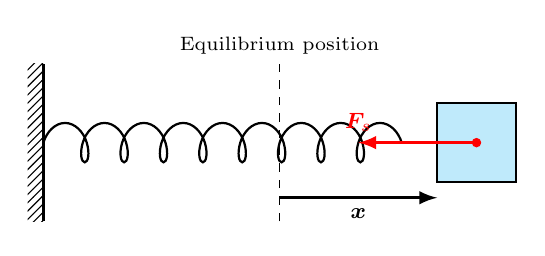
\begin{tikzpicture}
    \draw[mass] (5,.5) rectangle (6,1.5);
    \draw[thick,
      decoration={aspect=.6,segment length=5mm, amplitude=2.5mm, coil},
      decorate] (0,1)--(5,1);
    \fill[pattern=north east lines] (-.2,0) rectangle (0,2);
    \draw[thick] (0,.0)--(0,2);
    \fill[red] (5.5,1) circle (.06);
    \draw[vector,red] (5.5,1)--(4,1) node[above]{$\bm F_s$};
    \draw[dashed] (3,0)--(3,2) node[above]{\scriptsize Equilibrium position};
    \draw[vector] (3,.3)--(5,.3) node[midway,below]{$\bm x$};
  \end{tikzpicture}
  \hspace{.2in}
  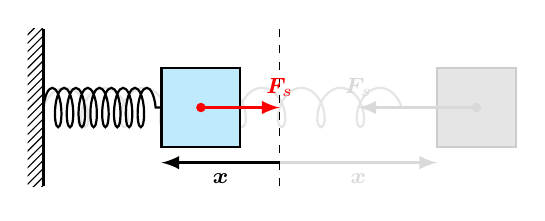
\begin{tikzpicture}
    \draw[thick,gray!40,fill=gray!20] (5,.5) rectangle (6,1.5);
    \draw[thick,gray!20,
      decoration={aspect=.6,segment length=5mm, amplitude=2.5mm, coil},
      decorate] (0,1)--(5,1);
    \fill[pattern=north east lines](-.2,0) rectangle (0,2);
    \draw[thick](0,.0)--(0,2);
    \fill[gray!30] (5.5,1) circle (.06);
    \draw[vector,gray!30] (5.5,1)--(4,1) node[above]{$\bm F_s$};
    \draw[dashed](3,0)--(3,2);
    \draw[vector,gray!30](3,.3)--(5,.3)node[midway,below]{$\bm x$};
    \draw[mass] (1.5,.5) rectangle (2.5,1.5);
    \draw[thick,
      decoration={aspect=.3,segment length=1.5mm, amplitude=2.5mm, coil},
      decorate] (0,1)--(1.5,1);
    \draw[vector] (3,.3)--(1.5,.3) node[midway,below]{$\bm x$};
    \fill[red] (2,1) circle (.06);
    \draw[vector,red] (2,1)--(3,1) node[above]{$\bm F_s$};
  \end{tikzpicture}
\end{figure}



\section{Free-Body Diagrams}

Acceleration (if there is going to be any at all) depends on net force
$\bm F_\text{net}$. Without a vector sum of all the forces, we cannot determine
the magnitude, direction of the acceleration, or how acceleration will evolve
in time. To help is visualiz forces acting on an object, we use
\textbf{free-body diagrams} (FBD) to represent all the forces. FBDs are a very
important standard technique when solving any dynamics problems, and is not
a step that should be skipped.

For \emph{rectilinear}, or \emph{translational} motion, FBDs are usually drawn
by assuming that all forces acting at the center of mass (``CM''),
represented by the ``big dot''. For example:
\begin{figure}[ht]
  \centering
  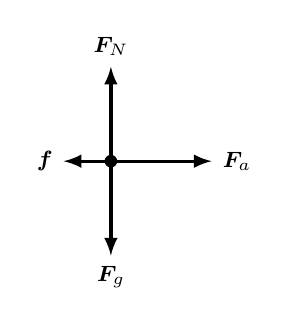
\begin{tikzpicture}[scale=.8]
    \fill (1.5,1) circle (.1);
    \draw[vector] (1.5,1)--(1.5,-.5) node[below]{$\bm F_g$};
    \draw[vector] (1.5,1)--(1.5,2.5) node[above]{$\bm F_N$};
    \draw[vector] (1.5,1)--(3.1,1) node[right]{$\bm F_a$};
    \draw[vector] (1.5,1)--(.75,1) node[left] {$\bm f$};
  \end{tikzpicture}
\end{figure}

However, for motion where \emph{rotation} is (at least) a possibility, we
must note that while gravitational force $\bm F_g$ acts at CM, normal
force $\bm F_N$, friction $\bm f$ and applied force $\bm F_a$ all act at the
point of contact, away from the CM. In those cases, forces should be drawn
where they are applied. For example, a sphere rolling down a ramp should have
weight $\bm F_g$, normal force $\bm F_N$ and static friction $\bm f_s$ acting
on it, as shown in Fig.~\ref{fig:rollingdown1}
\begin{figure}[ht]
  \centering
  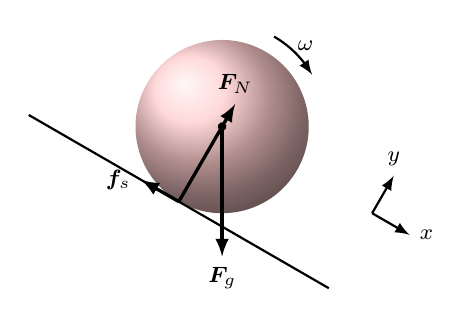
\begin{tikzpicture}[scale=1.1,rotate=-30]
    \shade[ball color=red!20] circle (1);
    \draw[thick] (-2,-1)--(2,-1);
    \fill circle (.05);
    \draw[vector,rotate=30] (0,0)--(0,-1.5) node[below]{$\bm F_g$};
    \draw[vector] (0,-1)--(0,.3) node[above]{$\bm F_N$};
    \draw[vector] (0,-1)--(-.5,-1) node[left]{$\bm f_s$};
    \draw[axes] (2,0)--(2.5,0) node[right]{$x$};
    \draw[axes] (2,0)--(2,.5) node[above]{$y$};
    \draw[axes] (0,1.2) arc (90:60:1.2) node[pos=.3,right]{$\omega$};
  \end{tikzpicture}
  \caption{Free-body diagram of a sphere rolling down a ramp without slipping}
  \label{fig:rollingdown1}
\end{figure}

Once the FBD is drawn, decide on the axes to help you solve the motion. One of
the axes should line up with the direction of motion. This guarantees that
the \emph{other} axis will not have any net force.

%\begin{frame}{Example Problem}
A more difficult static problem may involve two surfaces with two different
friction coefficients. For example, a ladder leaning on a wall. This problem
cannot be solved without first understanding rotational motion, but we can
still draw a FBD.

\textbf{Example:} A uniform ladder is \SI{5.0}{\metre} long and weighs
\SI{400}\newton. The ladder rests against a slippery vertical wall, as
shown in the figure. The inclination angle between the ladder and the rough
floor is \ang{53}. Find the reaction forces from the floor and
from the wall on the ladder and the coefficient of static friction $\mu_s$
at the interface of the ladder with the floor that prevents the ladder from
slipping.
\begin{center}
    \pic{.3}{../dynamics-calculus/graphics/ladder}
\end{center}




%\section{Multi-Body Problems}
%
%\begin{figure}[ht]
%  \pic1{../dynamics-calculus/graphics/worldslongestroadtrainwithpowertrailer8}
%  \caption{A road train that is common in Australia}
%  \label{fig:roadtrain}
%\end{figure}
%\begin{itemize}
%\item The objects are connected by a cable or a solid linkage with negligible
%  mass
%\item All objects (usually) have the same acceleration
%\item Require multiple free-body diagrams
%\end{itemize}
%
%
%
%To solve a connected-bodies problem, you can follow these procedures:
%\begin{enumerate}
%\item Draw a FBD on each of the objects
%\item Sum all the forces on all the objects along the direction of motion
%  \begin{itemize}
%  \item Direction of motion is usually very obvious
%  \item All internal forces should cancel and do not figure into the
%    acceleration of the system
%  \end{itemize}
%\item Compute the acceleration of the entire system using second law of motion
%  \begin{itemize}
%  \item Remember that (usually) every object has the same acceleration!
%  \end{itemize}
%\item Go back to the FBD of each of the objects and compute the unknown
%  forces (usually tension)
%\end{enumerate}
%
%
%
%%  \textbf{Example:} A tractor-trailer pulling two trailers starts from rest
%%  and accelerates with an acceleration $a$ on a straight, level road. The mass
%%  of the truck (T) is \SI{5450}{\kilo\gram}, the mass of the first trailer (A)
%%  is \SI{31500}{\kilo\gram}, and the mass of the second trailer (B) is
%%  \SI{19600}{\kilo\gram}.
%%  \begin{enumerate}
%%  \item What magnitude of force must the truck generate in order to accelerate
%%    the entire vehicle?
%%  \item What magnitude of force must each of the trailer hitches withstand
%%    while the vehicle is accelerating?
%%  \end{enumerate}
%%  Assume that frictional forces are negligible in comparison with the forces
%%  needed to accelerate the large masses.
%%
%
%
%
%%\begin{frame}{Different Types of Connected Bodies}
%Multiple objects pressed against one another. There may not be friction, but
%there are definitely action/reaction forces between the blocks.
%\begin{center}
%  \begin{tikzpicture}[scale=.8]
%    \draw[thick] (-3,0)--(4,0);
%    \draw[thick] rectangle (1,1) node[midway]{$m$};
%    \draw[thick] (1,0) rectangle (3,1.5) node[midway]{$M$};
%    \draw[vector] (-1.5,.5)--(0,.5) node[pos=0,left]{$\bm F_a$};
%  \end{tikzpicture}
%\end{center}
%Or multiple objects stacked on top of one another. The contact surface between
%$M$ and the floor may (or may not) have friction, while the surface between
%$M$ and $m$ must have a friction coefficient $\mu$.
%\begin{center}
%  \begin{tikzpicture}[scale=.8]
%    \draw[thick] (-1,0)--(5.5,0);
%    \draw[thick] rectangle (3,1.5) node[midway]{$M$};
%    \draw[thick] (.75,1.5) rectangle (2.25,2.5) node[midway]{$m$};
%    \draw[vector] (3,.5)--(4.5,.5) node[right]{$\bm F_a$};
%  \end{tikzpicture}
%\end{center}
%
%
%
%
%\subsection{Pulley Problems}
%
%\begin{figure}[ht]
%  \centering
%  \begin{tikzpicture}[scale=.7]
%    \draw[ultra thick,brown] (-1,-1.6)--(-1,0);
%    \draw[ultra thick,brown] (1,0)--(1,-3);
%    \draw[thick,fill=gray] circle (1.05);
%    \draw[thick,fill=gray!40] circle (.95);
%    \draw[line width=5.5] (0,-.15)--(0,2);
%    \draw[very thick] (-2,2)--(2,2);
%    \fill[white] circle (.1);
%    \draw[mass] (-1.5,-1.6) rectangle +(1,-1) node[midway]{$M$};
%    \draw[mass] (.5,-3) rectangle +(1,-1.4) node[midway]{$m$};
%  \end{tikzpicture}   
%\end{figure}
%
%An \textbf{Atwood machine} is made of two objects connected by a rope that
%runs over a pulley. The pulley allows the direction of force and direction
%of motion to change between two objects.
%    
%\textbf{Example:} The object on the left has a mass of $M$ and the object on
%the right has a mass of $m$.
%\begin{enumerate}
%\item What is the acceleration of the masses?
%\item What is the tension in the rope?
%\end{enumerate}
%  
%
%%%\begin{frame}{Example Problem: Atwood Machine}
%%  An \textbf{Atwood machine} is made of two objects connected by a rope that
%%  runs over a pulley. The pulley allows the direction of force and direction
%%  of motion to change between two objects.
%%  \begin{columns}
%%    \column{.35\textwidth}
%%    \centering
%%    \pic1{../dynamics-calculus/graphics/pulley_prob_2}
%%
%%    \column{.65\textwidth}
%%    \textbf{Example:} The object on the left has a mass of $M$ and the object
%%    on the right has a mass of $m$.
%%    \begin{itemize}
%%    \item What is the acceleration of the masses?
%%    \item What is the tension in the rope?
%%    \end{itemize}
%%  
%%
%
%
%
%%%\begin{frame}{A Difficult Problem!}
%%  \begin{columns}
%%    \column{.6\textwidth}
%%    \textbf{Example:} Two blocks of mass $m$ and $M$ are connected via pulley
%%    with a configuration as shown on the right. The coefficient of static
%%    friction between the left block and the surface is $\mu_{s,1}$, and the
%%    coefficient of static friction between the right block and the surface is
%%    $\mu_{s,2}$. Formulate a mathematical inequality for the condition that no
%%    sliding occurs. There may be more than one inequality. 
%%    
%%    \column{.4\textwidth}
%%    \pic{1}{../dynamics-calculus/graphics/pulley_prob_6}
%%  
%%
%%
%%
%%
%%%\begin{frame}{Multiple Pulleys}
%%  When there are multiple pulleys involved, we have to remember that tension
%%  force is distributed evenly along the cable.
%%
%%  \vspace{.2in}
%%  \begin{columns}
%%    \column{.6\textwidth}
%%    \textbf{Example:} A block of mass $m$ is pulled, via two pulleys as shown,
%%    at constant velocity along a surface inclined at angle $\theta$. The
%%    coefficient of kinetic friction is $\mu_k$, between block and surface.
%%    Determine the pulling force $F$. Ignore the mass of the pulleys. 
%%    
%%    \column{.4\textwidth}
%%    \pic{1}{../dynamics-calculus/graphics/pulley_prob_7}
%%    
%%
%
%
%%%\begin{frame}{One More!}
%%  \begin{columns}
%%    \column{.75\textwidth}
%%    \textbf{Example:} A block of mass $M$ is lifted at constant velocity, via
%%    an arrangement of pulleys as shown. Determine the pulling force $F$. Ignore
%%    the mass of the pulleys. 
%%
%%    \uncover<2>{
%%      \vspace{.2in}\textbf{Example:} The pulling force is replaced by a $10M$
%%      mass, and was let go. What are the accelerations of the $M$ and the
%%      $10M$ mass?
%%    }
%%    
%%    \pic{1}{../dynamics-calculus/graphics/pulley_prob_9}
%%  
%%
%
%
%%\begin{frame}{A More Typical Problem}
%More typically, an Atwood machine problem is one where two objects are
%sliding on a surface. These surfaces may have (or may not) have friction. In
%this example, two blocks are connected by a massless string over a
%frictionless pulley as shown in the diagram.
%\begin{figure}[ht]
%  \centering
%  \begin{tikzpicture}[scale=1.2]
%    \draw[thick,brown] (-4,.4)--(.1,.4);
%      \draw[thick] (0,0)--(-5.5,0) node[midway,below]{$\mu$};
%      \draw[thick,fill=magenta!20] (-4,0) rectangle (-5,.75) node[midway]{$m$};
%      \begin{scope}[rotate=-30,thick]
%        \draw[brown] (1,.4)--(-.05,.4);
%        \draw (0,0)--(3,0) node[midway,below left]{$\mu$};
%        \draw[mass] (1,0) rectangle (2.5,1) node[midway]{$M$};
%      \end{scope}
%      \begin{scope}[rotate=-15]
%        \draw[thick,fill=gray] (0,.3) circle (.15);
%        \draw[thick,fill=lightgray] (0,.3) circle (.1);
%        \draw[ultra thick] (0,0)--(0,.3);
%        \fill (0,.3) circle (.04);
%      \end{scope}
%      \draw[thick,gray!70] (0,0)--(0,-1.5);
%      \draw[axes] (0,-.5) arc (270:330:.5) node[midway,below]{$\phi$};
%  \end{tikzpicture}
%\end{figure}
%\begin{enumerate}
%\item Determine the acceleration of the blocks.
%\item Calculate the tension in the string.
%\end{enumerate}
%

%\section{Rigid Body Dynamics of Multiple Bodies}
\label{sec:multibody}


\begin{center}
  \pic{.7}{dynamics-calculus/graphics/worldslongestroadtrainwithpowertrailer8}
\end{center}
\begin{itemize}
\item The objects are connected by a cable or a solid linkage with negligible
  mass
\item All objects (usually) have the same acceleration
\item Require multiple free-body diagrams
\end{itemize}


\section{Introduction}
To solve a multi-body problem, you can follow these procedures:
\begin{enumerate}
\item Draw a FBD on each of the objects
\item Sum all the forces on all the objects along the direction of motion
  \begin{itemize}
  \item Direction of motion is usually very obvious
    \item All internal forces should cancel and do not figure into the
      acceleration of the system
  \end{itemize}
\item Compute the acceleration of the entire system using second law of motion
  \begin{itemize}
  \item Remember that (usually) every object has the same acceleration!
  \end{itemize}
\item Go back to the FBD of each of the objects and compute the unknown
  forces
\end{enumerate}

\section{Motion Along Level Surfaces}

\subsection{Objects Connected by Massless Cables}
Three masses ($m_1$, $m_2$ and $m_3$) are connected by massless
cables\footnote{Obviously cables are not \emph{literally} massless, but here,
we assume that the masses of the cables are insignificant compared to the
masses, and therefore we can ignore them without making our answers
inaccurate}, and pulled to the right by an external force $\vec F$ across a
level surface, as shown in Figure~\ref{fig:tension}. The coefficient of kinetic
friction between the masses and the surface is $\mu$.
\begin{figure}[ht]
  \centering
  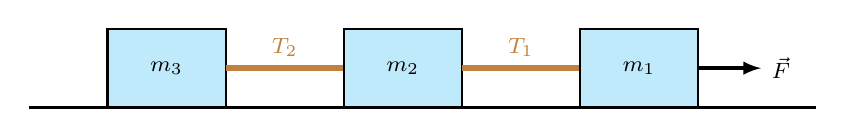
\begin{tikzpicture}
    \draw[thick] (0,0)--(10,0);
    \draw[mass] (1,0) rectangle (2.5,1) node[midway]{$m_3$};
    \draw[brown,line width=2] (2.5,.5)--(4,.5)
    node[midway,above]{$T_2$};
    \draw[mass] (4,0) rectangle (5.5,1) node[midway]{$m_2$};
    \draw[brown,line width=2] (5.5,.5)--(7,.5)
    node[midway,above]{$T_1$};
    \draw[mass] (7,0) rectangle (8.5,1) node[midway]{$m_1$};
    \draw[vector] (8.5,.5)--(9.3,.5) node[right]{$\vec F$};
  \end{tikzpicture}
  \caption{Three masses are connected by massless cables and accelerate
    together.}
  \label{fig:tension}
\end{figure}

For this example, we want to consider the following questions:
\begin{enumerate}[nosep,leftmargin=15pt]
\item What are the forces acting on each of the masses?
\item What is the acceleration of the system, assuming that the cables do not
  break?
\item What are the magnitudes of the tension forces ($T_1$ and $T_2$) in the
  two cables?
\end{enumerate}

\textbf{Step 1---Free-Body Diagrams:} Our first step to finding the solution to
the questions is to draw free-body diagrams for each of the masses, as shown in
Figure~\ref{fig:fbd1}.
\begin{figure}[ht]
  \centering
  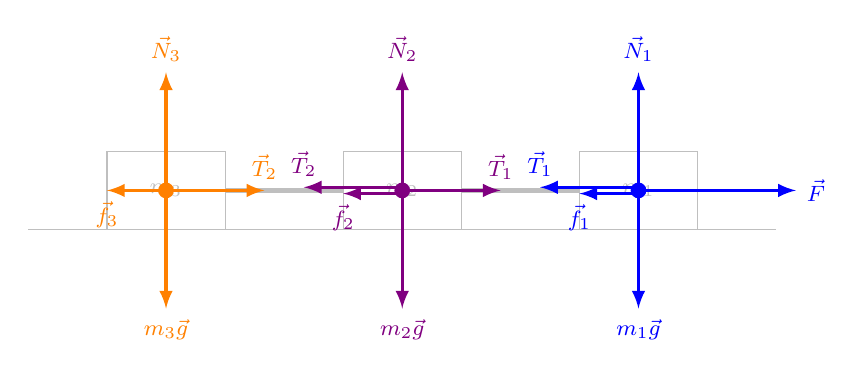
\begin{tikzpicture}[lightgray]
    \draw (0,0)--(9.5,0);
    \draw (1,0) rectangle (2.5,1) node[midway]{$m_3$};
    \draw[line width=2] (2.5,.5)--(4,.5);
    \draw (4,0) rectangle (5.5,1) node[midway]{$m_2$};
    \draw[line width=2] (5.5,.5)--(7,.5);
    \draw (7,0) rectangle (8.5,1) node[midway]{$m_1$};
    \begin{scope}[vector]
      \begin{scope}[orange]
        \fill (1.75,.5) circle (.1);
        \draw (1.75,.5)--(1.75,-1) node[below]{$m_3\vec g$};
          \draw (1.75,.5)--(1.75,2) node[above]{$\vec N_3$};
          \draw (1.75,.5)--(3,.5) node[above]{$\vec T_2$};
          \draw (1.75,.5)--(1,.5) node[below]{$\vec f_3$};
      \end{scope}
      \begin{scope}[violet]
        \fill (4.75,.5) circle (.1);
        \draw (4.75,.5)--(4.75,-1) node[below]{$m_2\vec g$};
        \draw (4.75,.5)--(4.75,2) node[above]{$\vec N_2$};
        \draw (4.75,.5)--(6,.5) node[above]{$\vec T_1$};
        \draw (4.75,.54)--(3.5,.54) node[above]{$\vec T_2$};
        \draw (4.75,.46)--(4,.46) node[below]{$\vec f_2$};
      \end{scope}
      \begin{scope}[blue]
        \fill (7.75,.5) circle (.1);
        \draw (7.75,.5)--(7.75,-1) node[below]{$m_1\vec g$};
        \draw (7.75,.5)--(7.75,2) node[above]{$\vec N_1$};
        \draw (7.75,.5)--(9.75,.5) node[right]{$\vec F$};
        \draw (7.75,.54)--(6.5,.54) node[above]{$\vec T_1$};
        \draw (7.75,.46)--(7,.46) node[below]{$\vec f_1$};
      \end{scope}
    \end{scope}
  \end{tikzpicture}
  \caption{Free-body diagrams}
  \label{fig:fbd1}
\end{figure}

In doing so, we note that
\begin{itemize}[nosep,leftmargin=15pt]
\item External force $\vec F$ is only applied to $m_1$, therefore it
  should not appear on the other free-body diagrams
\item Kinetic friction of the masses are: $f_1=\mu N_1=\mu m_1g$,
  $f_2=\mu N_2=\mu m_2g$, and $f_3=\mu N_3=\mu m_3g$. (In a general problem, the
  coefficients of friction do not need to be the same for all the masses, but
  we are simplifying the problem here.
\item $T_1$ and $T_2$ are action-reaction pair of forces
\end{itemize}


\textbf{Step 2---Second law of motion:} Once the free-body diagrams are
completed, we can sum the forces along the direction of motion for each object,
i.e.\ applying the second law of motion individually on each object.
\begin{align}
  {\color{blue} F-\mu m_1g-T_1} &= {\color{blue}m_1a}\label{eq:m1}\\
  {\color{orange} T_1-\mu m_2g-T_2} &= {\color{orange}m_2a}\label{eq:m2}\\
  {\color{violet} T_2-\mu m_3g} &= {\color{violet}m_3a}\label{eq:m3}
\end{align}
Since the cables do not break, all three masses have the same acceleration $a$
towards the right. Therefore we can \emph{sum} the three equations above
(Eqs.~\ref{eq:m1}--\ref{eq:m3}) to get the expression:
\begin{align}
  \nonumber
  F-\mu(m_1+m_2+m_3)g &= (m_1+m_2+m_3)a\\
  F-\mu Mg &= Ma \label{eq:law2-system}
\end{align}
which is just the second law of motion applied to the whole system as a single
object. Here, we introduce the variable $M=m_1+m_2+m_3$ to represent the total
mass of the whole system.

We can now use Eq.~\ref{eq:law2-system} to calculate the acceleration of the
entire system:
\begin{equation}
  a=\frac FM-\mu g
  \label{eq:accel}
\end{equation}
Depending on the problem, you may be solving for the algebraic expression, or
an actual numerical value.

\textbf{Step 3---Unknown Forces:} Once the acceleration of the system is known,
we can find all the other unknown forces---in this case, tension forces $T_1$
and $T_2$.

The easiest way is to solve for $T_2$ is to look at the force balance of
$\color{orange}m_3$ (Eq.~\ref{eq:m3}). Solving for $T_2$ and substituting the
acceleration that we got from Eq.~\ref{eq:accel}, we get:
\begin{align*}
  T_2&=m_3 a+\mu m_3 g\\
  &=m_3({\color{red}a}+\mu g)\\
  &=m_3\left({\color{red}\frac FM-\mu g}+\mu g\right)\\
  &=\frac{m_3}M F\\
  T_2 &=\frac{m_3}{m_1+m_2+m_3} F
\end{align*}
Then, to solve for $T_1$, we can use the force balance of $\color{blue}m_1$ in
Eq.~\ref{eq:m1}. Solving for $T_1$, and substituting the acceleration from
Eq.~\ref{eq:accel}, we find the expression for $T_1$:
\begin{align*}
  T_1 &=F-m_1({\color{red}a}+\mu g)\\
  &=F-m_1\left({\color{red}\frac FM-\mu g}+\mu g\right)\\
  &=F-m_1\frac FM\\
  &=\frac{M-m_1}MF\\
  T_1&=\left(\frac{m_2+m_3}{m_1+m_2+m_3}\right)F
\end{align*}
Of course, we can also use the force balance of $\color{violet}m_2$ to find
$T_1$. Solving for $T_1$ in Eq.~\ref{eq:m2}:
\begin{align*}
  T_1 &=T_2 + \mu m_2g + m_2a\\
  &=T_2 + m_2(a + \mu g)\\
  &=\frac{m_3}MF + m_2\left(\frac FM -\mu g + \mu g\right)\\
  &=\frac{m_2+m_3}MF\\
  &=\left(\frac{m_2+m_3}{m_1+m_2+m_3}\right)F\\
\end{align*}
which is the same as before.

But there is yet another way to find $T_1$! This time we treat
$\color{violet}m_2$ and $\color{orange}m_3$ as a single object. In this case, we add Eqs.~\ref{eq:m2} and \ref{eq:m3} together, and then solving for $T_1$
and substituting acceleration from Eq.~\ref{eq:accel}:
\begin{align*}
  T_1& =(m_2+m_3)(a+\mu g)\\
  & =(m_2+m_3)(\frac FM-\mu g+\mu g)\\
  & =\frac{m_2+m_3}MF\\
  & =\frac{m_2+m_3}{m_1+m_2+m_3}F\\
\end{align*}
Which, not surprisingly, is the same answer as using the other two methods.
Ultimately, the multi-problem is an exercise that you have done many times
in your math classes: solving multiple equations with multiple unknowns. In
this case, there are 3 unknowns ($a$, $T_1$ and $T_2$) and 3 equations.

\newpage
\subsection{Another Connected Bodies Example}
Two masses ($m_1$ and $m_2$) are being pushed along a level surface by an
external applied force $\vec F$, as shown in Figure~\ref{fig:pushed}. The
coefficient of kinetic friction between the masses and the surface is $\mu$.
Like the previous example, we want to consider the following questions:
\begin{enumerate}[nosep,leftmargin=15pt]
\item What is the acceleration of the masses?
\item What is the normal force that $m_1$ exerts on $m_2$?
\end{enumerate}
This problem is very similar to the previous example.

\begin{figure}[ht]
  \centering
  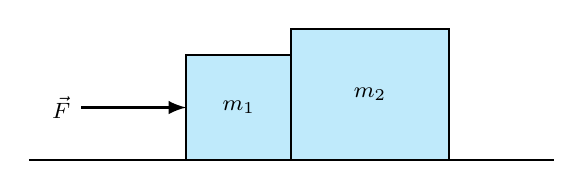
\begin{tikzpicture}[scale=4/3]
    \draw[thick] (-1.5,0)--(3.5,0);
    \draw[mass] rectangle (1,1) node[midway]{$m_1$};
    \draw[mass] (1,0) rectangle (2.5,1.25) node[midway]{$m_2$};
    \draw[vector] (-1,.5)--(0,.5) node[pos=0,left]{$\vec F$};
  \end{tikzpicture}
  \caption{Two masses pushed together by an external force}
  \label{fig:pushed}
\end{figure}

\textbf{Step 1---Free-body diagrams:} Like the previous problem, we start with
drawing free-body diagrams for each of the masses, shown in
Figure~\ref{fig:fbd-pushed}.
\begin{figure}[ht]
  \centering
  \begin{subfigure}{.4\textwidth}
    \centering
    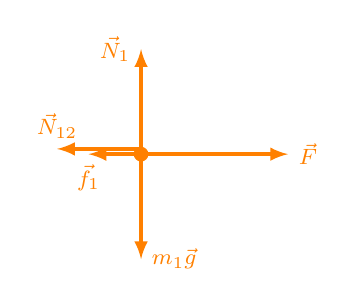
\begin{tikzpicture}[scale=4/3,orange,vector]
      \fill circle (.07);
      \draw (0,0)--+(1.4,0) node[right]{$\vec F$};
      \draw (0,0)--+(0,-1) node[right]{$m_1\vec g$};
      \draw (0,0)--+(0,1) node[left]{$\vec N_1$};
      \draw (0,.05)--+(-.8,0) node[above]{$\vec N_{12}$};
      \draw (0,0)--+(-.5,0) node[below]{$\vec f_1$};
    \end{tikzpicture}
    \subcaption{Mass $m_1$}
  \end{subfigure}
  \begin{subfigure}{.4\textwidth}
    \centering
    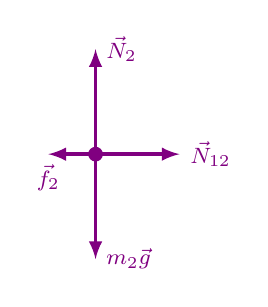
\begin{tikzpicture}[scale=4/3,vector,violet]
      \fill circle (.07);
      \draw (0,0)--+(0,1) node[right]{$\vec N_2$};
      \draw (0,0)--+(-.45,0) node[below]{$\vec f_2$};
      \draw (0,0)--+(0,-1) node[right]{$m_2\vec g$};
      \draw (0,0)--+(.8,0) node[right]{$\vec N_{12}$};
    \end{tikzpicture}
    \subcaption{Mass $m_2$}
  \end{subfigure}
  \caption{Free-body diagrams for the pushed-blocks example}
  \label{fig:fbd-pushed}
\end{figure}

There are a few details about the normal forces.
\begin{itemize}[nosep,leftmargin=15pt]
\item All normal forces ($N_1$, $N_2$ and $N_{12}$) appear in the free-body
  diagrams as if they only act on the centre of mass. In fact, the normal force
  is spread over the entire contact surface.
\item The normal force $\vec N_{12}$ is at the contact between the two masses.
  It is an action-reaction pair, similar to the tension force in the previous
  example. When $m_1$ pushes against $m_2$ (action), $m_2$ pushes back against
  $m_1$ (reaction).
\end{itemize}  


\textbf{Step 2--Second law of motion:} Using the free-body digrams, we then sum
forces along the direction of motion for each mass:
\begin{align}
  {\color{orange}F-N_{21}-\underbrace{\mu m_1g}_{f_1}} &={\color{orange}m_1a} \\
  {\color{violet}N_{12}-\underbrace{\mu m_2g}_{f_2}} &= {\color{violet}m_2a}
\end{align}
Again, we recognize that both masses must have the acceleration. Adding them
together, we have
\begin{align}
  \nonumber
  F - \mu(m_1+m_2)g  &= (m_1+m_2)a\\
  F - \mu Mg  &= Ma \label{eq:system}
\end{align}
where $M=m_1+m_2$ is the total mass of the system of objects.
Eq.~\ref{eq:system} is essentially the second law of motion applied to the
entire system as if it is a single object. Solving for acceleration, we have:
\begin{equation}
  a= \frac FM- \mu g
  \label{eq:accel2}
\end{equation}
Eq.~\ref{eq:accel2} is identical to Eq.~\ref{eq:accel} from our first example.
Again, like the last problem, acceleration can be expressed as an algebraic
expression or with numerical values depending on the problem.

\textbf{Step 3--Find remaining forces:} Once acceleration is known, we can find
the remaining unknown force: the normal force $N_{12}$ between the blocks.
The magnitude of the normal force $N_{12}$ can be calculated using the
force-balance equations of either mass. Using the equation for $M_1$ and solving
for $N_{12}$:
\begin{align*}
  N_{12} &= F- m_1({\color{red}a}+\mu g)\\
  &= {\color{blue}F} - m_1\left({\color{red}\frac FM-\mu g} +\mu g\right) \\
  &= {\color{blue}M\frac FM} - m_1\left(\frac FM\right) \\
  &= \frac{M-m_1}M F\\
  N_{12}&= \frac{m_2}{m_1+m_2} F
\end{align*}
Or we can apply the same procedure to the force balance for $m_2$:
\begin{align*}
  N_{12} &= m_2 ({\color{red}a} + \mu g) \\
  &= m_2 \left({\color{red}\frac FM-\mu g} + \mu g\right) \\
  &= m_2 \left(\frac FM\right) \\
  &= \frac{m_2}{m_1+m_2} F
\end{align*}
which is the same as before.

\newpage
\subsection{Stacked Objects}
Two blocks ($m_1$ and $m_2$) are stacked on top of each other above a
frictionless table, as shown in Figure~\ref{fig:stacked}. An external force
$\vec F$ is applied to $m_2$, causing both blocks to accelerate to the right
together without slipping. The coefficients of static and kinetic friction
between the masses are $\mu_s$ and $\mu_k$ respectively.
\begin{figure}[ht]
  \centering
  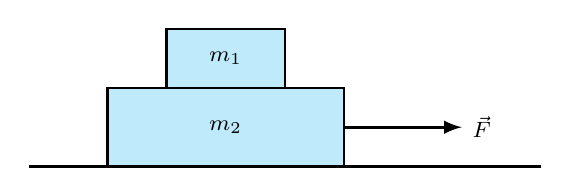
\begin{tikzpicture}
    \draw[thick] (-1,0)--(5.5,0);
    \draw[mass] rectangle (3,1) node[midway]{$m_2$};
    \draw[mass] (.75,1) rectangle (2.25,1.75) node[midway]{$m_1$};
    \draw[vector] (3,.5)--(4.5,.5) node[right]{$\vec F$};
  \end{tikzpicture}
  \caption{Two masses stacked on top of each other on a frictionless table.}
  \label{fig:stacked}
\end{figure}

We want to consider the following questions:
\begin{enumerate}[nosep,leftmargin=12pt]
\item What is the maximum acceleration of the masses without slipping?
\item What is the magnitude of the external force $F$ at maximum
  acceleration?
\item What is the acceleration of $m_1$ if $F$ exceeds this maximum value?
\end{enumerate}


\textbf{Step 1--Free-body diagrams:} As in the previous example, we draw
free-body diagrams of both masses.
\begin{figure}[ht]
  \centering
  \begin{subfigure}{.4\textwidth}
    \centering
    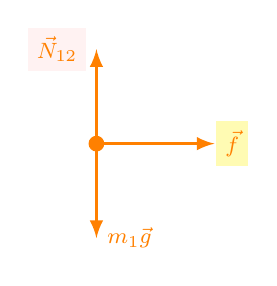
\begin{tikzpicture}[orange,vector]
      \fill (1.5,1.375) circle (.1);
      \draw (1.5,1.375)--+(1.5,0) node[right,fill=yellow!30]{$\vec f$};
      \draw (1.5,1.375)--+(0,-1.2) node[right]{$m_1\vec g$};
      \draw (1.5,1.375)--+(0,1.2)  node[left=3,fill=pink!20]{$\vec N_{12}$};
    \end{tikzpicture}
  \end{subfigure}
  \begin{subfigure}{.4\textwidth}
    \centering
    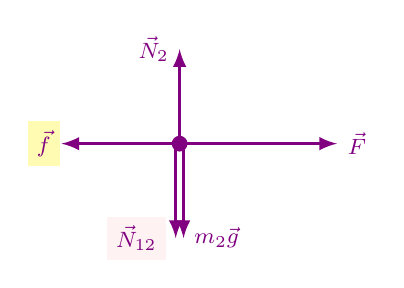
\begin{tikzpicture}[vector,violet]
      \fill (1.5,.5) circle (.1);
      \draw (1.5,.5)--+(2,0) node[right]{$\vec F$};
      \draw (1.5,.5)--+(-1.5,0) node[left,fill=yellow!30]{$\vec f$};
      \draw (1.55,.5)--+(0,-1.2) node[right]{$m_2\vec g$};
      \draw (1.45,.5)--+(0,-1.2) node[left=3,fill=pink!20]{$\vec N_{12}$};
      \draw (1.5,.5)--+(0,1.2) node[left]{$\vec N_2$};
    \end{tikzpicture}
  \end{subfigure}
\end{figure}
There are two action-reaction pairs of forces:
\begin{itemize}
\item Normal force $N_{12}$ at the interface between $m_1$ and $m_2$ acts upwards
  on $m_1$ and downwards on $m_2$
\item Static friction\footnote{That is, if the blocks don't slide against each
other. If they do, then the friction would be kinetic friction instead} $f$,
  also at the interface between $m_1$ and $m_2$, acts forward on $m_1$, and
  backwards on $m_2$.
\end{itemize}
$f$ is the force that actually accelerates $m_1$ forward! (Think about
what happens when there is no friction between the masses.)


\textbf{Step 2:} For problems like this, we focus on the top blocks first.
The force that pulls the block forward is the static friction force $f_s$.
The second law of motion applied to $m_1$ is:
%  \vspace{.1in}
%  \begin{columns}
%    \column{.25\textwidth}
%    \centering
%    \begin{tikzpicture}[scale=.95,vector,orange]
%      \fill circle (.08);
%      \draw (0,0)--(1.5,0) node[right]{$\vec f_s$};
%      \draw (0,0)--(0,-1.2) node[right]{$m_1\vec g$};
%      \draw (0,0)--(0,1.2) node[left]{$\vec N_{12}$};
%    \end{tikzpicture}
%
Summing the forces along the direction of motion:
\begin{equation}
  f = m_1a
\end{equation}
Maximum acceleration $a_\text{max}$ occurs when static friction is also at
maximum, i.e.\ $f=\max f_s=\mu_s N_{12}=\mu_s m_1g$:
\begin{align}
  \nonumber
  \mu_s m_1g &= m_1a_\text{max}\\
  a_\text{max} &=\mu_s g
\end{align}
We see that the maximum acceleration is, in fact, independent of mass.

\textbf{Step 3:} Once the $a_\text{max}$ is known, we can use it to calculate
the maximum applied force. We can do this by substituting the expression for
acceleation into the force balance for $m_2$:
\begin{align*}
  F_\text{net}=F_\text{max}-f &= m_2a_\text{max}\\
  F_\text{max} &= m_2a_\text{max}+f_s\\
  &= m_2(\mu_sg)+\mu_s m_1g\\
  F_\text{max} &=\mu_s(m_1+m_2)g
\end{align*}
Or treat the whole system as a single object with total mass of $m_1+m_2$:
\begin{align}
  \nonumber
  F_\text{max} &= (m_1+m_2)a_\text{max}\\
  &= \mu_s(m_1+m_2)g
\end{align}
Of course both ways gives you the same answer.

\section{Atwood Machine--Pulley Problems}

\subsection{Example Problem: Atwood Machine}
An \textbf{Atwood machine} is made of two objects connected by a rope that
runs over a pulley. The pulley allows the direction of force and direction
of motion to change between two objects.
%  \begin{columns}
%    \column{.35\textwidth}
%    \begin{center}
%      \pic1{graphics/pulley_prob_2}
%    \end{center}
%    \column{.65\textwidth}
%    \textbf{Example:} The object on the left has a mass of $M$ and the object
%    on the right has a mass of $m$.
%    \begin{itemize}
%    \item What is the acceleration of the masses?
%    \item What is the tension in the rope?
%    \end{itemize}
%  \end{columns}


%  More typically, an Atwood machine problem is one where two objects are
%  sliding on a surface. These surfaces may have (or may not) have friction. In
%  this example, two blocks are connected by a massless string over a
%  frictionless pulley as shown in the diagram.
\begin{figure}[ht]
  \centering
  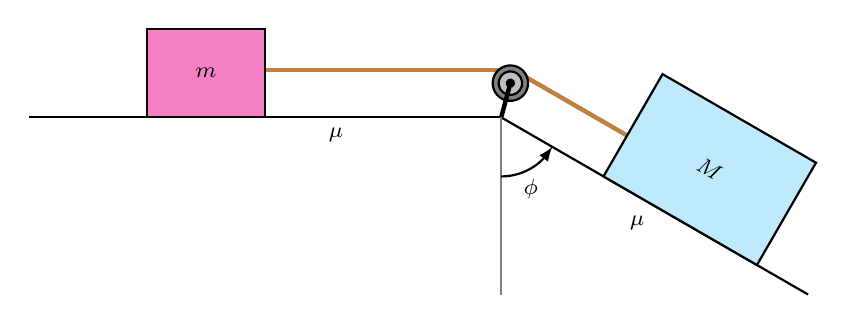
\begin{tikzpicture}[scale=1.5,thick]
    \draw[ultra thick,brown] (-2,.4)--(.1,.4);
    \draw (0,0)--(-4,0) node[pos=.35,below]{$\mu$};
    \draw[fill=magenta!50] (-2,0) rectangle +(-1,.75) node[midway]{$m$};
    \begin{scope}[rotate=-30]
      \draw[ultra thick,brown] (1,.4)--(-.05,.4);
      \draw (0,0)--(3,0) node[midway,below left]{$\mu$};
      \draw[mass] (1,0) rectangle (2.5,1) node[midway,rotate=-30]{$M$};
    \end{scope}
    \begin{scope}[rotate=-15]
      \draw[fill=gray] (0,.3) circle (.15);
      \draw[fill=lightgray] (0,.3) circle (.1);
      \draw[ultra thick] (0,0)--(0,.3);
      \fill (0,.3) circle (.04);
      \end{scope}
    \draw[gray] (0,0)--(0,-1.5);
    \draw[->] (0,-.5) arc(270:330:.5) node[midway,below]{$\phi$};
  \end{tikzpicture}
\end{figure}
%  \begin{enumerate}[(a)]
%  \item Determine the acceleration of the blocks.
%  \item Calculate the tension in the string.
%  \end{enumerate}
%\end{document}
%

%\chapter{Work and Energy}
\label{chapter:energy}

We start with some definition at are (unfortunately) not very useful:
\begin{itemize}
\item \textbf{Energy} is the ability to do work.
\item \textbf{Work} is the mechanism in which energy is transformed.
\end{itemize}
At a minimum, these definitions at least tell two things:
\begin{itemize}
\item The concepts of work and energy cannot be separated: Defining work
  without leading to energy is rather pointless; defining energy without first
  referring to work makes no sense.
\item Word definitions are not enough. We also need to have \emph{mathematical}
  definitions as well.
\end{itemize}
It is customary to start with the definition of mechanical work, and use it
to define different forms of energies.

\section{Mechanical Work}
\label{sec:mechwork}
An infinitesimal amount of \textbf{mechanical work} $\dl W$ is done when a
force $\mathbf F$ displaces an object by an infinitesimal amount
$\dl\mathbf x$. If the force moves an object along the path $\mathcal C$, the
total work $W$ done by the force is defined by the integral:
\begin{equation}
  \boxed{
    W=\int_{\mathcal C}\dl W=\int_{\mathcal C}\mathbf F(\mathbf x)\cdot\dl\mathbf x
  }
  \label{work-definition}
\end{equation}
While both force and displacement are vectors, work is a scalar quantity. Work
by $\bm F$ can be positive or negative depending on the dot product. In
general, the amount of work done ($W$) depends on the path $\mathcal C$. %From
%Eq.~(\ref{work-definition}), we recognize that
No work is done if the force is perpendicular to displacement, (i.e.\
$\bm F\cdot\dl\bm x=0$) which means that the force did not \emph{cause} the
displacement, or if the object does not move, (i.e.\ $\dl\bm x=\bm 0$), or if
no force is applied during motion (i.e.\ $\bm F=\bm 0$).

For motion confined to one direction along a one-dimensional coordinate
system, Eq.~(\ref{work-definition}) reduces to\footnote{Note that direction
still matters for $F$ and $x$, even in 1D, in that there is still a positive
and negative direction (if $F$ and $\dl x$ are in the same direction, then
$W>0$; and if $F$ and $\dl x$ are in opposite direction, then $W<0$).}:
\begin{equation}
  \boxed{
    W=\int_{x_0}^{x_1} F(x)\dl x
  }
\end{equation}
For a constant force that moves an object along a straight path, the integral
simplifies to just the dot product of two vectors\endnote{We must remember how
  to express the dot products. If you know the angles between the vectors,
  then:
  \begin{equation*}
    \bm A\cdot\bm B= AB\cos\theta
  \end{equation*}
  And if you know the components of the vectors, then
  \begin{equation*}
    \bm A\cdot\bm B= A_xB_x+A_yB_y+A_zB_z
  \end{equation*}
}:
\begin{equation}
  \boxed{
    W = \bm F\cdot\Delta\bm x=F\Delta x\cos\theta
  }
  \label{eq:no-integration}
\end{equation}
where $\theta$ is the angle between the force and displacement vectors. We can
also use the above equation if the force $\bm F$ is \emph{averaged} over
the displacement, i.e.\
\begin{equation}
  \bm F=\bm F_\text{avg}=\frac{\int F(x)\dl x}{\Delta x}
\end{equation}
At this moment, it is unclear what the force $\bm F$ is. Whereas we use the
\emph{net force} when calculating acceleration in dynamics problems, when
calculating the work done by ``a force'', it could mean:
\begin{enumerate}[leftmargin=12pt]
\item\textbf{Work done by a \emph{specific} force.} There may be multiple
  forces acting on an object. We can calculate, based on the motion of the
  object, how much work is done by each force. Calclating the work done by a
  specific force allows us to study the exact mechanism in how energy is
  transformed.
  
\item\textbf{Work done by the \emph{net} force}, in other words, the \emph{sum}
  of all the work done by each force. This is also called the \textbf{net work}
  $W_\text{net}$:
  \begin{equation*}
    W_\text{net}
    = \sum_i W_i
    =\int_{\mathcal C}\bm F_\text{net}(x)\cdot\dl\bm x
  \end{equation*}
  The net work allows us to study what is the overall conservation of energy
  to the entire object.
\end{enumerate}

\fcolorbox{black}{yellow!10}{
  \small
  \begin{minipage}{.97\linewidth}
    \textbf{A simple example}: a worker pushes a heavy crate up a ramp with a
    varying applied force. The free-body diagram for this problem is shown
    below. Here, four forces act on the crate: gravity $\bm F_g$, normal force
    $\bm F_n$, kinetic friction $\bm f$, and applied force $\bm F_a(x)$, which
    is expressed as a function of the crate's displacement as it moves.
    \begin{center}
      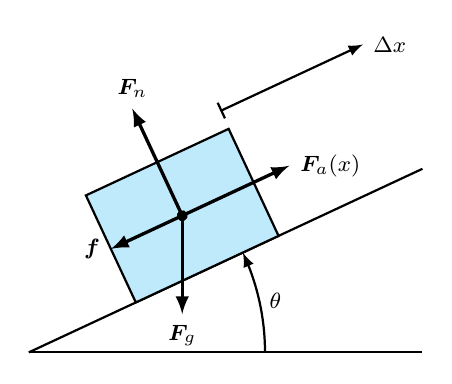
\begin{tikzpicture}
        \draw[thick] (0,0)--(5,0);
        \draw[axes] (3,0) arc (0:25:3) node[midway,right]{$\theta$};
        \begin{scope}[rotate=25]
          \draw[thick] (0,0)--({5/cos(25)},0);
          \draw[thick,|->] (3.5,1.75)--+(2,0) node[right]{$\Delta x$};
          \draw[mass] (1.5,0) rectangle (3.5,1.5);
          \fill (2.5,.75) circle (.07);
          \draw[vector] (2.5,.75)--+(1.5,0) node[right]{$\bm F_a(x)$};
          \draw[vector] (2.5,.75)--+(0,1.5) node[above]{$\bm F_n$};
          \draw[vector,rotate around={-25:(2.5,.75)}]
          (2.5,.75)--+(0,-1.25) node[below]{$\bm F_g$};
          \draw[vector] (2.5,.75)--+(-1,0) node[left]{$\bm f$};
        \end{scope}
      \end{tikzpicture}
    \end{center}
    We can calculate the work done by each force:
    \begin{itemize}[leftmargin=12pt]
    \item Work done by the normal force is zero, because $\bm F_n$ is
      perpendicular to the direction of motion:
      \begin{equation*}
        W_n=\int\underbrace{\bm F_n\cdot\dl\bm x}_{=0}=0
      \end{equation*}
    \item Work done by kinetic friction is negative, because $\bm f$ is in the
      opposite direction to motion: %and therefore the dot product gives a $-1$.
      \begin{equation*}
        W_f=\int\bm f\cdot\dl\bm x=-\int f\dl x=-\mu_k F_n\Delta x<0
      \end{equation*}
    \item Work done by gravity is also negative, because the component of
      gravity along the direction of motion is in the opposite direction. (This
      is badly written!!)
    \item The work done by the applied force is positive, because applied force
      is in the same direction as motion.
      \begin{equation*}
        W_a(x)=\int_{x_0}^x F_a\dl x>0
      \end{equation*}
    \end{itemize}
    The total work (i.e.\ the net work) done by summing the work done by each
    force:
    \begin{align*}
      W_\text{net} &=W_a+W_n+W_g +W_f\\
      &=\int\left(\bm F_a+\bm F_n+\bm F_g+\bm F_f\right)
      \cdot\dl\bm x =\int\bm F_\text{net}\cdot\dl\bm x
    \end{align*}
  \end{minipage}
}


\section{Kinetic Energy}
\label{sec:transKE}
When a net force acts on an object (with constant mass) to accelerate it, work
is done, For motion in one dimension, the total/net work done is given by:
\footnote{When you do this problem ``properly'' in 2D or 3D, the only
difference is the dot product, which only \emph{slightly} increases the
complexity of the problem from the 1D case:
\begin{equation*}
  W_\text{net}
  = \int\bm F_\text{net}(\bm x)\cdot\dl\bm x
  = \cdots = m\int\bm v\cdot\dl\bm v
\end{equation*}
The difference in the dot product is a lot easier to evaluate than you might
think:
\begin{align*}
  m\int\bm v\cdot\dl\bm v
  &=m\left(\int v_x\dl v_x + \int v_y\dl v_y + \int v_z\dl v_z\right)\\
  &=\left(\frac12mv_x^2+\frac12mv_y^2 + \frac12mv_z^2\right)
  =\frac12mv^2
\end{align*}
where $v^2=v_x^2+v_y^2+v_z^2$. This is, of course, the same result that we
got from the one-dimensional case.}
\begin{equation}
  W_\text{net}
  =\int_{x_0}^{x_1}F_\text{net}(x)\dl x
  =\int ma\dl x
  =m\int\diff vt\dl x
\end{equation}
Since both $v(t)$ and $x(t)$ are continuously differentiable in time, we can
switch the order of the differentiation:
\begin{equation*}
  =m\int\diff xt\dl v=m\int_{v_0}^{v_1}v\dl v
\end{equation*}
The limits of integration switch from the initial and final position ($x_0$ and
$x_1$) to the initial and final velocities, where $v_0=v(x_0)$ and
$v_1=v(x_1)$. Evaluating this integral, we have:
\begin{equation*}
  =m\int_{v_0}^{v_1}v\dl v
  =\frac12mv^2\Big|^{v_1}_{v_0}
  =\frac12mv_1^2-\frac12mv_0^2
  =\Delta K
\end{equation*}
where $K$ is defined as the \textbf{kinetic energy}\footnote{This is more
specifically called the \emph{translational} kinetic energy, and it should be
distinguished from the \emph{rotational kinetic energy} which is used when an
object is rotating about a pivot.}:
\begin{equation}
  \boxed{
    K=\frac12mv^2
  }
\end{equation}
The definition of kinetic energy came from this integration: when the net force
on an object is doing work, that work is equal to the change in
\emph{something}, and we \emph{define} that quantity as the kinetic energy.
This is known as the \textbf{work-energy theorem}\footnote{Also known as the
\textbf{work-energy principle}, and \textbf{work-energy relationship}}:
\begin{equation}
  \boxed{
    W_\text{net}=\Delta K
  }
  \label{work-energy-theorem}
\end{equation}
When multiple forces act on an object, \emph{positive} net work will
\emph{increase} the kinetic energy of the object, while \emph{negative} net
work will decreases kinetic energy. Eq.~(\ref{work-energy-theorem}) applies
regardless of \emph{what} the net force is comprised of. Very importantly, the
work-energy theorem turns a potentially difficult integration problem
(integrating $W_\text{net}$) into a simple algebraic expression ($\Delta K$).


%  \textbf{Example 1:} A net force $F=4x$ (in newtons) acts on an object of mass
%  \SI2{\kilo\gram} as it moves along the $x$-axis from $x=1$ to $x=\SI5\metre$.
%  Given that the object is at rest at $x=1$,
%  \begin{enumerate}[(a)]
%  \item Calculate the net work
%  \item What is the final speed of the object?
%  \end{enumerate}


\section{Potential Energy}

Unlike kinetic energy, forms of energy that can be stored are called
\textbf{potential energy}.

\subsection{Gravitational Force \& Gravitational Potential Energy}
Consider an object that is dropped (free-falling) under the force of gravity
over a distance of $\Delta x$, shown in Fig.~\ref{fig:falling1}.
\begin{figure}[ht]
  \centering
  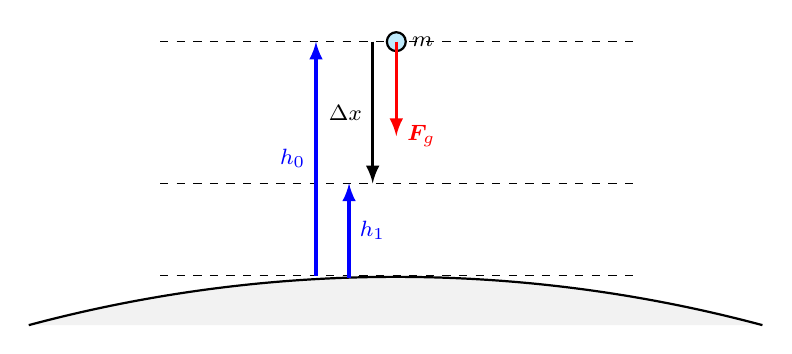
\begin{tikzpicture}[scale=.6]
    \draw[thick,fill=gray!10] (7.75,0) arc (75:105:30);
    \draw[dashed] (-5,1.05)--+(10,0);
    \draw[dashed] (-5,6)--+(10,0);
    \draw[dashed] (-5,3)--+(10,0);
    \draw[mass] (0,6) circle (.2) node[right=2]{$m$};
    \draw[vector,red] (0,6)--+(0,-2) node[right]{$\bm F_g$};
    \draw[vector] (-.5,6)--+(0,-3) node[midway,left]{$\Delta x$};
    \draw[vector,blue] (-1.7,1.05)--+(0,4.95) node[midway,left]{$h_0$};
    \draw[vector,blue] (-1,1)--+(0,2) node[midway,right]{$h_1$};
  \end{tikzpicture}
  \caption{Gravitational force doing positive work on a free-falling object.}
  \label{fig:falling1}
\end{figure}

When displacement $\Delta\bm x$ is small, acceleration due to gravity
$\bm g$ can be considered to be constant, therefore
$\bm F_g=m\bm g$ is a constant force. Work done by gravity can be
calculated using Eq.~\ref{eq:no-integration}, and no integration is needed.
Since both $\bm F_g$ and $\Delta\bm x$ are in the same direction, work
done by gravity ($W_g$) is positive. From the work-energy theorem
(Eq.~\ref{work-energy-theorem}), there is an increase in kinetic energy, and
the object speeds up:
\begin{equation*}
  W_g=mg\Delta x>0 \quad\longrightarrow\quad \Delta K > 0
\end{equation*}
This is consistent with our understanding of kinematics and dynamics. But the
work done by gravitational force can also be expressed in terms of the change
in height. Using ground as the reference level (i.e.\ $h=0$), the work done by
gravity can be written as:
\begin{equation*}
  W_g = mg(h_0-h_1)
\end{equation*}
We can further modify this equation:
\begin{align}
  W_g &= mg(h_0-h_1)\nonumber\\
  & = -mg(h_1-h_0)\nonumber\\
  & = -(mgh_1-mgh_0)\nonumber\\
  W_g &= -\Delta U_g
\end{align}
where $U_g$ is defined as the \textbf{gravitational potential energy}:
\begin{equation}
  \boxed{U_g=mgh}
\end{equation}
Since the choice of the reference level (where we define $h=0$) is arbitrary,
we are more interested in the \emph{change} in gravitational potential energy,
which is related to the work done by gravity:
\begin{equation}
  \boxed{
    W_g=-\Delta U_g
  }\quad\text{where}\quad
  \boxed{
    \Delta U_g=mg\Delta h
  }
  \label{work-potential-energy}
\end{equation}
In Eq.~\ref{work-potential-energy}, we note some special relationships between
the work done by gravity ($W_g$) and the change in the gravitational potential
energy ($U_g$):

\fcolorbox{black}{yellow!10}{
  \begin{minipage}{.95\textwidth}
    \begin{itemize}[nosep,leftmargin=10pt]
    \item \emph{Positive} work by gravity \emph{decreases} gravitational
      potential energy, while
    \item \emph{Negative} work by gravity \emph{increases} gravitational
      potential energy
    \item Work by gravity is \emph{path independent}: $W_g$ depends on the end
      points $h_0$ and $h_1$, but not \emph{how} it goes from
      $h_0\rightarrow h_1$
    \item Only work done by gravity can affect $U_g$
    \end{itemize}
  \end{minipage}
}

As you can see in the example in Fig.~\ref{path-independence}, the work done by
gravity is the same in all cases. That is not to say that there are no other
forces acting on the object; we have merely isolated the work done by the
gravitational force alone.
\begin{figure}[ht]
  \centering
  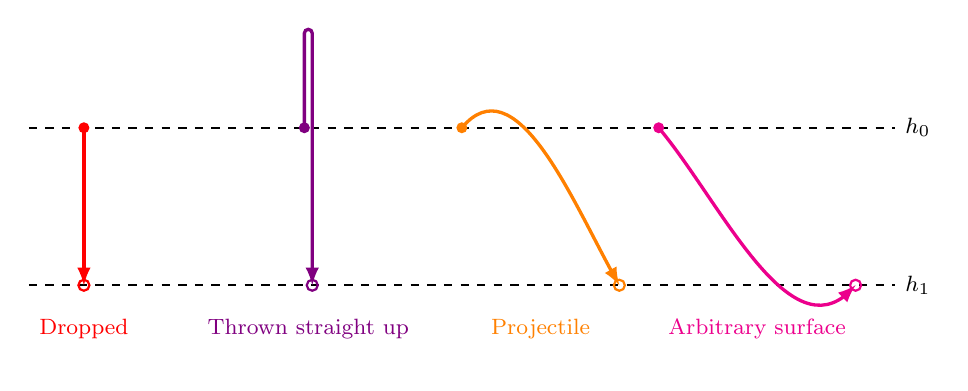
\begin{tikzpicture}
    \draw[thick,dashed] (0,0)--+(11,0) node[right]{$h_0$};
    \draw[thick,dashed] (0,-2)--+(11,0) node[right]{$h_1$};
    
    \fill[red] (.7,0) circle (.07);
    \draw[vector,red] (.7,0)--+(0,-2);
    \draw[thick,red] (.7,-2) circle (.07);
    \node[below,red] at (.7,-2.3){Dropped};
    
    \fill[violet] (3.5,0) circle (.07);
    \draw[vector,violet] (3.5,0)--+(0,1.2) arc(180:0:.05)--+(0,-3.2);
    \draw[thick,violet] (3.6,-2) circle (.07);
    \node[below,violet] at (3.55,-2.3){Thrown straight up};
      
    \fill[orange] (5.5,0) circle (.07);
    \draw[vector,orange] (5.5,0) to[out=50,in=120] +(2,-2);
    \draw[thick,orange] (7.5,-2) circle (.07);
    \node[below,orange] at (6.5,-2.3){Projectile};
      
    \fill[magenta] (8,0) circle (.07);
    \draw[vector,magenta] (8,0) to[out=-50,in=230] +(2.5,-2);
    \draw[thick,magenta] (10.5,-2) circle (.07);
    \node[below,magenta] at (9.25,-2.3){Arbitrary surface};
  \end{tikzpicture}  
  \caption{Work done by gravity ($W_g$) is the same in all above cases because
    they all have the same initial and final height.}
  \label{path-independence}
\end{figure}



\subsection{Law of Universal Gravitation}

\begin{figure}[ht]
  \centering
  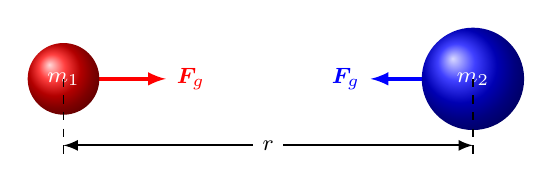
\begin{tikzpicture}[scale=.65]
    \draw[vector,red] (0,0)--(2,0) node[right]{$\bm F_g$};
    \draw[vector,blue] (8,0)--(6,0) node[left]{$\bm F_g$};
    \shade[balloon1] circle (.7) node[white]{$m_1$};
    \shade[balloon2] (8,0) circle (1) node[white]{$m_2$};
    \draw[dashed] (0,0)--(0,-1.5);
    \draw[dashed] (8,0)--(8,-1.5);
    \draw[<->,thick] (0,-1.3)--(8,-1.3) node[midway,fill=white]{$r$};
  \end{tikzpicture}
  \caption{Gravity is a mutual attraction between massive objects}
\end{figure}

\textbf{Gravity} is the mutually attractive force between
massive objects. The magnitude of gravitational force between two
\textbf{point masses} is proportional to their masses ($m_1$, $m_2$), and
inversely proportional to the square of the distance ($r$) between them:
\begin{equation}
  \boxed{F_g=\frac{Gm_1m_2}{r^2}}
\end{equation}
where $G=\SI{6.67e-11}{N.m^2/kg^2}$ is the \textbf{universal gravitational
  constant}



%\begin{frame}{Universal Gravitation}
%  \begin{itemize}
%  \item If $m_1$ exerts a force $\bm F_g$ on $m_2$, then $m_2$ also exerts a
%    force $-\bm F_g$ on $m_1$. The attractive forces are equal in magnitude
%    and opposite in direction (third law of motion).
%  \item $m_1$ and $m_2$ are \emph{point masses} that do not occupy any space
%  \item For objects with \emph{spatial extend}\footnote{It means that the mass
%    actually takes up space}, the law assumes that one object is not inside the
%    other
%  \end{itemize}
%\end{frame}
%
%
%
%\begin{frame}{A Simple Example Problem}
%  \textbf{Example:} A \SI{65.0}{\kilo\gram} astronaut is walking on the surface
%  of the moon, which has a mean radius of \SI{1.74e3}{\kilo\metre} and a mass
%  of \SI{7.35e22}{\kilo\gram}. What is the weight of the astronaut?
%\end{frame}
%
%
%
%\begin{frame}{Example Problem}
%  \textbf{Example:} How far apart would you have to place two
%  \SI{7.0}{\kilo\gram} bowling balls so that the force of gravity between them
%  would be \SI{1.25e-8}\newton?
%
%  \vspace{.5in}Notice the magnitude of gravitational force between the two
%  objects. In fact, gravitational force is the weakest of all fundamental
%  forces.
%\end{frame}
%
%
%
%\begin{frame}{Relating Gravitational Field \& Gravitational Force}
%  When a mass $m$ is placed inside a gravitational field $\bm g$, it
%  experiences a gravitational force given by the familiar equation:
%  %$\bm g$ itself doesn't do anything unless another mass $m$ is inside this
%  %field. At which point, the other mass $m$ experiences a gravitational force
%  %related to $\bm g$ by:
%  
%  \eq{-.1in}{
%    \boxed{\bm F_g=m\bm g}
%  }
%
%  Regardless of what generated the gravitational field. When there are multiple
%  source masses, the total gravitational field is the vector sum of all the
%  gravitational fields from each source mass.
%
%  \eq{-.1in}{
%    \bm g =\bm g_1+\bm g_2+\bm g_3+\bm g_4+\cdots
%  }
%\end{frame}



The expression for \textbf{gravitational potential energy} can be obtained
from the law of universal gravitation using basic integral calculus:

\begin{equation}
  W_g = \int_{\bm r_1}^{\bm r_2}\bm F_g\cdot\dl\bm r
  = Gm_1m_2 \int_{r_1}^{r_2}\frac{\dl r}{r^2} = -\Delta U_g
\end{equation}
where we again define the gravitational potential energy stored between two
point masses $m_1$ and $m_2$:
\begin{equation}
  \boxed{U_g=-\frac{Gm_1m_2}r}
\end{equation}
$U_g$ is the work required to move two objects from $r$ to $\infty$. $U_g=0$ at
$r=\infty$ and \emph{decrease} as $r$ decreases




%\begin{frame}{Gravitational Potential Energy}
%  Since $g$ is not a constant, we use an equation consistent with the law of
%  universal gravity to obtain the general expression for
%  \textbf{gravitational potential energy} stored between a system of two
%  masses:
%  
%  \eq{-.05in}{
%    \boxed{U_g=-\frac{Gm_1m_2}r}
%  }
%  \begin{center}
%    \begin{tabular}{l|c|c}
%      \rowcolor{pink}
%      \textbf{Quantity} & \textbf{Symbol} & \textbf{SI Unit} \\ \hline
%      Gravitational potential energy & $U_g$ & \si\joule \\
%      Point masses & $m_1$, $m_2$ & \si{\kilo\gram} \\
%      Distance between centres of mass & $r$ & \si\metre \\
%      Universal gravitational constant & $G$ & \si{N.m^2/kg^2}
%    \end{tabular}
%  \end{center}
%  The ``reference level'' is chosen at infinity (i.e.\ $U_g=0$ at $r=\infty$)
%  and \emph{decrease} as $r$ decreases
%\end{frame}




As we look at work done by other forces, we will begin to see the same pattern
emerge for other forces.

\subsection{Spring Force \& Elastic Potential Energy}
The \textbf{spring force} $\bm F_s$ is the force that a
compressed/stretched spring exerts on the object connected to it, shown in
Fig.~\ref{hooke1}. An \emph{ideal} spring obeys \textbf{Hooke's law}, which
states that the spring force on a compressed/stretched spring is proportional
to the amount of spring displacement $\bm x$, and acts in the opposition
to the displacement:
\begin{equation}
  \boxed{
    \bm F_s=-k\bm x
  }
\end{equation}
The constant $k$ is called the \textbf{spring constant}\footnote{The spring
constant is also called the \textbf{force constant}, \textbf{Hooke's constant},
and in many engineering textbooks, \textbf{spring rate}.}, with a unit of
\emph{newton per meter} (\si{\newton\per\metre}). The spring constant depends
on the geometry of the spring, as well as the material that it is made of.
\begin{figure}[ht]
  \centering
  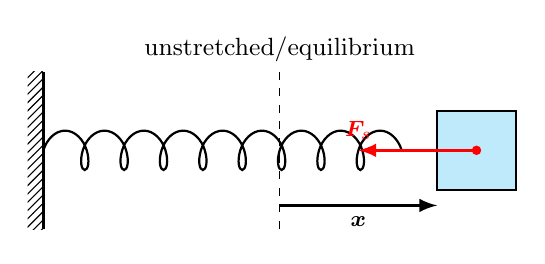
\begin{tikzpicture}
    \draw[mass] (5,.5) rectangle (6,1.5);
    \draw[thick,
      decoration={aspect=.6,segment length=5mm, amplitude=2.5mm, coil},
      decorate] (0,1)--(5,1);
    \fill[pattern=north east lines] (-.2,0) rectangle (0,2);
    \draw[thick] (0,.0)--(0,2);
    \fill[red] (5.5,1) circle (.06);
    \draw[vector,red] (5.5,1)--(4,1) node[above]{$\bm F_s$};
    \draw[dashed] (3,0)--(3,2) node[above]{\small unstretched/equilibrium};
    \draw[vector] (3,.3)--(5,.3) node[midway,below]{$\bm x$};
  \end{tikzpicture}
  \hspace{.2in}
  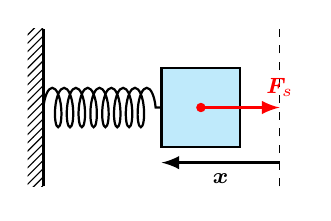
\begin{tikzpicture}
    \fill[pattern=north east lines] (-.2,0) rectangle (0,2);
    \draw[thick] (0,0)--(0,2);
    \draw[dashed] (3,0)--(3,2);
    \draw[mass] (1.5,.5) rectangle (2.5,1.5);
    \draw[thick,decorate,
      decoration={aspect=.3,segment length=1.5mm, amplitude=2.5mm, coil}]
    (0,1)--(1.5,1);
    \draw[vector] (3,.3)--(1.5,.3) node[midway,below]{$\bm x$};
    \fill[red] (2,1) circle (.06);
    \draw[vector,red] (2,1)--(3,1) node[above]{$\bm F_s$};
  \end{tikzpicture}
  \caption{Direction of spring force is always opposite to spring
    displacement.}
  \label{hooke1}
\end{figure}

As the spring force moves a mass connected to the spring, the work done by
the spring force is:
\begin{equation}
  W_s=\int_{x_0}^{x_1}F_s\dl x =-k\int_{x_0}^{x_1} x\dl x
  =-\frac12kx^2\Big|^{x_1}_{x_0}=-\Delta U_s
  \label{eq:spring-pot1}
\end{equation}
where $U_s$ is now defined as the \textbf{elastic potential energy}:
\begin{equation}
  \boxed{
    U_s=\frac12kx^2
  }
\end{equation}
Crucially, the work done by the spring force is related to the elastic
potential energy by:
\begin{equation}
  \boxed{
    W_s=-\Delta U_s
  }
\end{equation}
The integration in Eq.~\ref{eq:spring-pot1} shows the same properties as in
the work done by gravitational force.

\fcolorbox{black}{yellow!10}{
  \begin{minipage}{.95\textwidth}
    \begin{itemize}[nosep,leftmargin=10pt]
    \item \emph{Positive} work by the spring \emph{decreases} spring potential
      energy, while
    \item \emph{Negative} work by the spring \emph{increases} spring potential
      energy
    \item Work by the spring force is \emph{path independent:} $W_s$ depends on
      the end points $x_0$ and $x_1$, but not \emph{how} it moves from $x_0$ to
      $x_1$
    \item Only work done by $\bm F_s$ can affect $U_s$
    \end{itemize}
  \end{minipage}
}


\subsection{Electrostatic Force \& Electric Potential Energy}
Similar to the attractive force between masses, there is also a mutually
attractive or repulsive force between charged particles, given by
\textbf{Coulomb's law}:
\begin{equation}
  \boxed{
    \bm F_q=\frac{kq_1q_2}{r^2}\hat{\bm r}
  }
\end{equation}

The integral is nearly identical to that for the gravitational force:
\begin{equation}
  W_q=\int\bm F_q\cdot\dl\bm r
  =kq_1q_2\int_{r_0}^{r_1}\frac{\dl r}{r^2}
    =-\frac{kq_1q_2} r\Big|^{r_2}_{r_1}=-\Delta U_q
\end{equation}
where $U_q$ is the \textbf{electric potential energy} that is stored between
the two point charges, defined as:
\begin{equation}
  \boxed{
    U_q = \frac{kq_1q_2}r
  }
\end{equation}

Again, we see the same properties that we have observed 

\fcolorbox{black}{yellow!10}{
  \begin{minipage}{\textwidth}
    \begin{itemize}[nosep,leftmargin=10pt]
    \item\emph{Positive} work by the electric force \emph{decreases} electric
      potential energy, while
    \item\emph{Negative} work by the electric force \emph{increases} electric
      potential energy
    \item $W_q$ depends on the end points $r_0$ and $r_1$, but not \emph{how}
      it went from $r_0\rightarrow r_1$
    \item Only work done by $\bm F_q$ can affect $U_q$
    \end{itemize}
  \end{minipage}
}


\section{Conservative Forces}

These forces are called \textbf{conservative forces}
\begin{itemize}[nosep]
\item Gravitational force $\bm F_g$
\item Spring force $\bm F_s$
\item Electrostatic force $\bm F_q$
\item Magnetic force $\bm F_m$
\item Nuclear forces
\end{itemize}
Because they shared these common properties:
\begin{itemize}[nosep]
\item The work done by these forces relate to a change of a potential energy
  \begin{itemize}[nosep]
  \item Positive work decreases this related potential energy
  \item Negative work increases this related potential energy
  \end{itemize}
\item The work done by a conservative force is \emph{path independent}, in that
  it depends only on end points, but not \emph{how} it gets from one end point
  to the other
\end{itemize}



By the fundamental theorem of calculus, any conservative forces $\bm F$
must be the negative gradient of the potential energies:
\begin{equation}
  \boxed{
    \bm F=-\nabla U=-\diffp Ux\iii-\diffp Uy\jjj-\diffp Uz\kkk
  }
\end{equation}
In one-dimension, the gradient operator becomes just:
\begin{equation}
  \boxed{
    F=-\diff Ux
  }
\end{equation}
The direction of a conservative force \emph{always} decreases the potential
energy. (Pay attention to the negative sign. Students often forget it.)



\section{Energy Diagrams}
A plot of potential energy ($U$) vs.\ position ($x$) for a conservative force
\begin{figure}[ht]
  \centering
  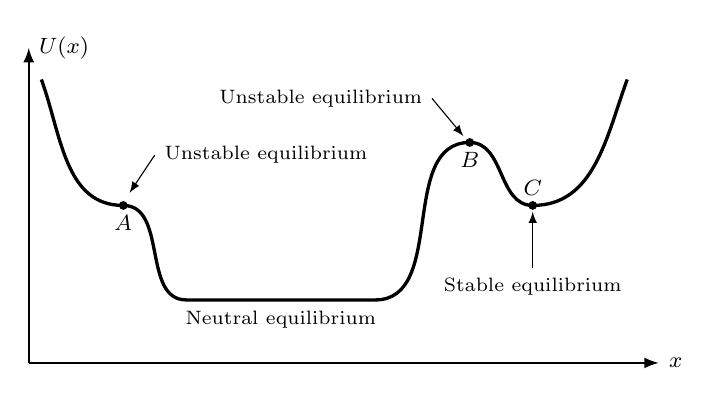
\begin{tikzpicture}[scale=.8]
    \draw[axes] (0,0)--(10,0) node[right]{$x$};
    \draw[axes] (0,0)--(0,5) node[right]{$U(x)$};
    \draw[very thick] (.2,4.5) to[out=-70,in=180](1.5,2.5)
    to[out=0,in=180] (2.5,1)
    --(5.5,1) node[midway,below]{\scriptsize Neutral equilibrium}
    to[out=0,in=180] (7,3.5)
    to[out=0,in=180] (8,2.5)
    to[out=0,in=250] (9.5,4.5);
    \fill(1.5,2.5) circle (.07) node[below]{$A$};
    \fill(7,3.5) circle (.07) node[below]{$B$};
    \fill(8,2.5) circle (.07) node[above]{$C$};
    \draw[<-] (1.6,2.7)--(2,3.3) node[right]{\scriptsize Unstable equilibrium};
    \draw[<-] (6.9,3.6)--(6.4,4.2) node[left]{\scriptsize Unstable equilibrium};
    \draw[<-] (8,2.4)--(8,1.5) node[below]{\scriptsize Stable equilibrium};
  \end{tikzpicture}
\end{figure}

%  The expressions for potential energies also come from integrating the work
%  equation, in that work equals to the change in \emph{something}, and we
%  called that potential energy. Therefore:
%
%  \eq{-.2in}{
%    \boxed{
%      W_c=-\Delta U
%    }
%  }
%  \begin{itemize}
%  \item\vspace{-.15in}$\Delta U$ can be positive or negative depending on the
%    direction of the (conservative) force
%  \item Positive work \emph{decreases} the related potential energy
%  \item Negative work \emph{increases} the related potential energy
%  \end{itemize}

%  Positive work done by conservative forces on an object does two things:
%  \begin{enumerate}[1.]
%  \item Decrease its potential energy, while
%  \item Increase its kinetic energy by the same amount
%  \end{enumerate}
%  Mathematically, this shows that mechanical energy must \emph{always} be
%  conserved when there are only conservative forces:
%
%  \eq{-.1in}{
%    W_c=-\Delta U = \Delta K \quad\longrightarrow\quad
%    \Delta K + \Delta U =0
%  }
%
%  That's why those forces are called conservative forces, and they form the
%  basis for conservation of energy.


\section{Non-Conservative Forces}
%The majority of forces are \textbf{non-conservative}.
The majority of the common forces encountered in introductory physics courses
are generally \textbf{non-conservative}. They include, but not limited to:
\begin{itemize}[nosep]
\item Applied force
\item Tension force
\item Normal force
\item Static friction
\item Kinetic friction
\item Aerodynamic lift and drag 
\end{itemize}
The work-energy theorem (Eq.~\ref{work-energy-theorem}) still applies for
non-conservative forces. However, the work done by non-conservative forces
differs from conservative forces in that:
\begin{itemize}
\item There is \textbf{no related potential energies}: the work done by a
  non-conservative force transform energy from one form of kinetic energy to
  another
\item The work is \textbf{path dependent}
\end{itemize}


\subsection{Work by Static Friction}
We can illustrate the work done by a non-conservative force in general, by
examining how work is done by static friction, using a multi-body problem
commonly studied in dynamics.

Two blocks with masses $m_1$ and $m_2$, stacked vertically, move to the right
without slipping by an external applied force $\bm F$ applied to $m_1$, as
shown in Fig.~\ref{stacked1}. The coefficient of static friction between the
two blocks is $\mu_s$, but the contact between $m_1$ and the table is
frictionless.\footnote{The focus of the dynamics study is often to calculate the
maximum acceleration $\bm a_\text{max}$ of the blocks without them sliding
against each other, and the maximum applied force $\bm F_\textbf{max}$
associated with that maximum acceleration.} The focus of \emph{this} example is
to find the work done by the forces between the blocks as the blocks accelerate.
\begin{figure}[ht]
  \centering
  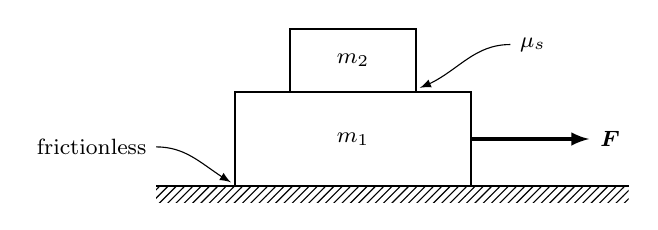
\begin{tikzpicture}
    \fill[pattern=north east lines] rectangle (6,-.2);
    \draw[thick] (0,0)--(6,0);
    \draw[thick] (1,0) rectangle (4,1.2) node[midway]{$m_1$};
    \draw[thick] (1.7,1.2) rectangle (3.3,2) node[midway]{$m_2$};
    \draw[vector] (4,.6)--+(1.5,0) node[right] {$\bm F$};
    \draw[<-] (.95,.05) to[out=150,in=0] (0,.5) node[left]{frictionless};
    \draw[<-] (3.35,1.25) to[out=20, in=180] (4.5,1.8) node[right]{$\mu_s$};
  \end{tikzpicture}
  \caption{An external force is applied to accelerate two stacked blocks to
    the right.}
  \label{stacked1}
\end{figure}

The free-body diagrams of the blocks are shown in Fig.~\ref{stacked-fbd}.
(The forces highlighted in the same colour are action-reaction pairs.) The
static friction between $m_1$ and $m_2$ is $\bm f$.
\begin{figure}[ht]
  \centering
  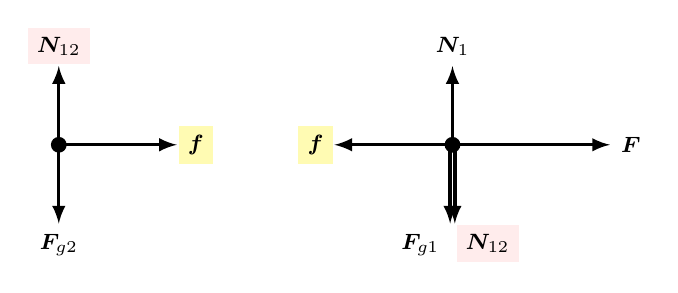
\begin{tikzpicture}
    \fill circle (.1);
    \draw[vector] (0,0)--(0,-1) node[below]{$\bm F_{g2}$};
    \draw[vector] (0,0)--(0, 1) node[above,fill=pink!30]{$\bm N_{12}$};
    \draw[vector] (0,0)--(1.5,0) node[right,fill=yellow!30]{$\bm f$};

    \fill (5,0) circle (.1);
    \draw[vector] (4.97,0)--+(0,-1) node[below left]{$\bm F_{g1}$};
    \draw[vector] (5.03,0)--+(0,-1)
    node[below right,fill=pink!30]{$\bm N_{12}$};
    \draw[vector] (5,0)--+(0,1) node[above]{$\bm N_1$};
    \draw[vector] (5,0)--+(-1.5,0) node[left,fill=yellow!30]{$\bm f$};
    \draw[vector] (5,0)--+(2,0) node[right]{$\bm F$};
  \end{tikzpicture}
  \caption{Free-body diagrams of the stacked masses.}
  \label{stacked-fbd}
\end{figure}

The top block $m_2$ accelerates to the right because there is static
friction $\bm f$ at the interface with $m_1$. Static friction is the
\emph{only} force doing work on $m_2$, and the work done by $\bm f$ is
\emph{positive}. $m_2$ gains kinetic energy, consistent with the work-energy
theorem (Eq.~\ref{work-energy-theorem}). The change in kinetic energy in $m_2$
as it moves from $x_0\longrightarrow x_1$ is
\begin{equation*}
  \Delta K_2=\int_{x_0}^{x_1} f\dl x
\end{equation*}
On the bottom block $m_1$, as it moves to the right, applied force $\bm F$
does positive work, while static friction $\bm f$ does \emph{negative}
work. At a minimum, we conclude that energy is transferred from $m_1$ to $m_2$,
but we can do a more thorough (although still very simple) analysis to find out
how much.

Without friction between $m_1$ and $m_2$, the net force on $m_1$ would have
just been the applied force $\bm F$, and the change in kinetic energy after
moving from $x_0\longrightarrow x_1$ to the right would have been simply
\begin{equation*}
  \Delta K_1 = \int_{x_0}^{x_1} F\dl x\quad\quad\text{(no friction)}
\end{equation*}
But with static friction present, the gain in kinetic energy is reduced:
\begin{equation*}
  \Delta K_1 = \int_{x_0}^{x_1} F_\text{net}\dl x =
  \int_{x_0}^{x_1} (F-f)\dl x = \int_{x_0}^{x_1} F\dl x -
  \underbrace{\int_{x_0}^{x_1} f\dl x}_{\Delta K_2}
\end{equation*}
Work done by static friction reduced the kinetic energy of $m_1$ by the same
amount that is gained by $m_2$. We therefore conclude that work done by
friction transfers kinetic energy from one block to another.


\section{Internal/Thermal Energy}
Consider a container of gas of mass $M$ moving at speed $v$ at a height $h$
above Earth (shown in Fig.~\ref{fig:gas}). It has a bulk kinetic energy of
\begin{equation*}
  K=\dfrac12 Mv^2
\end{equation*}
and a gravitational potential energy\footnote{Using the ground level as the
reference} of
\begin{equation*}
  U_g=Mgh
\end{equation*}
But the random motion of the air molecules also contribute to additional
energy, called the \textbf{internal energy} $E_\text{int}$, or
\textbf{thermal energy}.
\begin{figure}[ht]
  \centering
  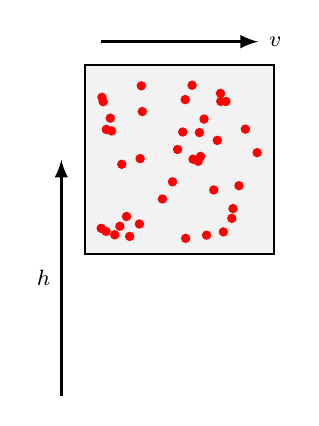
\begin{tikzpicture}
    \draw[thick,fill=gray!10] (-.2,-.2) rectangle (2.2,2.2);
    \draw[vector] (0,2.5)--(2,2.5) node[right]{$v$};
    \draw[vector] (-.5,-2)--(-.5,1) node[midway,left]{$h$};
    \foreach \i in {1,...,40} \fill[red] (rand+1,rand+1) circle (.06);
  \end{tikzpicture}
  \caption{A container of gas moving above Earth has kinetic, gravitational
    potential, as well as internal energies}
  \label{fig:gas}
\end{figure}
Internal energy of a system of molecules is the sum of all their kinetic and
potential energies at the microscopic level:
\begin{equation*}
  E_\text{int}=K_\text{micro} + U_\text{micro}
\end{equation*}
As the name suggests, $E_\text{int}$ is proportional to molecules'
\textbf{absolute temperature}, measured in \emph{kelvin}.
%\endnote{For those who are keen to know, for a
%monatomic or ideal gas, the internal energy comes entirely from the kinetic
%energy from the 3 degrees to translational freedom, and is given by
%\begin{equation*}
%  E_\text{int}=\dfrac32Nk_bT
%\end{equation*}
%where $N$ is the number of molecules, $k_b$ is the Boltzmann's constant. For a
%diatomic gas, there are 3 degrees of translational freedom, and 2 degrees of
%rotational freedom, and the internal energy is given by:
%\begin{equation*}
%  E_\text{int}\approx\dfrac52NkT
%\end{equation*}
%For solids, there are 3 degrees of translational freedom, and 3 degrees of
%degrees of vibrational freedom, and therefore the internal energy is:
%\begin{equation*}
%  E_\text{int}\approx3Nk_bT
%\end{equation*}
%}
Discussions on thermal/internal energy and the behaviour of gases and solids
are part of a much larger discipline within physics called
\textbf{thermodynamics}, but it is outside the scope of this chapter.



\section{Law of Conservation of Energy}
Conservation of energy is most often stated using a statement that even a lay
person with no physics background watching a movie may be familiar with:
\begin{center}
  \fcolorbox{black}{cyan!10}{
    \begin{minipage}{.98\linewidth}
      \centering
      \textbf{Energy cannot be created or destroyed; it only changes in form.}
    \end{minipage}
  }
\end{center}
While this statement certainly is not incorrect (indeed, it captures the
essence of how energy is conserved), the actual \textbf{law of conservation of
  energy} is more nuanced, and can be boring exercise in bookkeeping:
\begin{center}
  \fcolorbox{black}{cyan!10}{
    \begin{minipage}{.98\linewidth}
      \textbf{The change in the total energy of a system is equal
        to the net external work done to the system.}
    \end{minipage}
  }
\end{center}
Mathematically, the equation for the law of energy conservation is very
simple:
\begin{equation}
  \boxed{
    \Delta E_\text{sys}=W_\text{ext}
  }
  \label{eq:energy-conservation-law}
\end{equation}


\subsection{System}
A \emph{system} of object is defined in the same way as in solving dynamics
problems (specifically, the multi-body problems studied in
Section~\ref{sec:multibody}): a predefined collection of objects that apply
forces on each other, and therefore may do work on each other. A system may be:
\begin{itemize}[leftmargin=12pt,topsep=0pt]
\item\textbf{Isolated:} All the forces that act on the objects in the system
  act on each other (third law of motion) and are therefore \emph{internal}.
  There are no external forces.
\item\textbf{Closed:} There are external forces, but they do not do any work.
\item\textbf{Open:} There are external forces, and they do mechanical work
  (``external work'') to the objects in the system
\end{itemize}

The system's energy include both all the kinetic and potential energies of the
objects (collectively known as the \textbf{mechanical energy}), as well as the
internal/thermal energies of the objects:
\begin{equation}
  \boxed{
    E_\text{sys}
    =\underbrace{\sum K+\sum U}_\text{mechanical energy}+\sum E_\text{int}
  }
  \label{eq:system-energy}
\end{equation}
Substituting the expression from Eq.~(\ref{eq:system-energy}) into
(\ref{eq:energy-conservation-law}), we get the ``change'' in system energy:
\begin{equation}
  \boxed{
    \Delta E_\text{sys}=\sum\Delta K + \sum\Delta U + \sum\Delta E_\text{int}
    =W_\text{ext}
  }
\end{equation}
The sign convention of the external work $W_\text{ext}$ is the same as how it
is defined in Section~\ref{sec:mechwork}. When external work is: 
\begin{itemize}[leftmargin=12pt,nosep]
\item\textbf{Positive}: work is done \text{to} the system; the system
  energy \emph{increases}
\item\textbf{Negative}: work is done \text{by} the system to the surrounding;
  the system energy \emph{decreases}
\end{itemize}
In isolated systems that does not interact with the outside (and therefore
no external work can be done to the system), the law of conservation of energy
further simplifies to
\begin{equation}
  \boxed{
    \Delta E_\text{sys}=\sum\Delta K+\sum\Delta U+\sum\Delta E_\text{int}=0
  }
\end{equation}

%  In almost all of the problem encountered in AP Physics C, there will be no
%  change in the internal energy of the system, and conservation of energy
%  reduces to:
%  
%  \eq{-.1in}{
%    \boxed{ \Delta K + \Delta U = W_\text{ext} }\quad\rightarrow\quad
%    \boxed{ U_1 + K_1 + W_\text{ext} = U_2 + K_2 }
%  }
%
%  An \textbf{isolated system} is a system of objects that does not interact with
%  the surrounding. Think of an isolated system as a bunch of objects inside an
%  insulated box.
%  \begin{center}
%    \begin{tikzpicture}[scale=.7]
%      \fill[pattern=north east lines] rectangle (5,4);
%      \draw[thick] rectangle (5,4);
%      \draw[thick,fill=blue!5](.2,.2) rectangle (4.8,3.8);
%      \draw[thick,
%        decoration={aspect=.3,segment length=2mm, amplitude=2.5mm, coil},
%        decorate] (2.5,3.8)--(2.5,2.2) node[midway,right]{$\;\;k$};
%      \draw[thick,fill=cyan](2,2.25) rectangle (3,1.25) node[midway]{$m$};
%    \end{tikzpicture}
%  \end{center}
%  Since the system is isolated from the surrounding environment, the
%  environment can't do any work on it. Likewise, the energy inside the system
%  cannot escape either.


\subsection{Gravity: Free Fall}
Assuming that there are no friction and drag (i.e.: air resistance, see
Section~\ref{sec:drag}), a free-falling object (shown in Fig.~\ref{fig:earth})
forms an isolated system with Earth. 
\begin{figure}[ht]
  \centering
  \begin{tikzpicture}[scale=.65]
    \draw[thick,fill=cyan!5] (7.75,0) arc (75:105:30);
    \draw[mass] (0,4) circle (.2) node[right=3]{$m$};
    \draw[vector,red] (0,4)--+(0,-2) node[below=-2]{$\bm F_g$};
  \end{tikzpicture}
  \caption{Isolated system with a mass and Earth}
  \label{fig:earth}
\end{figure}
This isolated system consists of only Earth and the mass $m$, and therefore the
energy of the system is the kinetic energy of the mass ($K$) and the
gravitational potential energy ($U_g$) stored between the mass and
Earth\footnote{$U_g$ is often described as ``the gravitational potential energy
of the object''. Strictly speaking, this is incorrect; this is a topic that
will be studied in more detail in Chapter~\ref{chapter:gravity}. However, this
will not affect how the calculations is done, and in the opinion of the author,
poses no major conceptual issue. You are, of course, welcome to disagree}.

As the object falls, the gravitational force (which is internal to the system)
is doing positive work on both the mass as well as Earth\footnote{Due to the
mass of Earth, its displacement due to this gravitational force is laughably
insignificant. We will therefore only focus on the motion of the mass}.
%Beginning
%with the work-energy theorem, we recognize that as the object falls, the only
%force that does work is gravity, and it is \emph{internal} to the system.

Since gravity is a conservative force, the work done transforms gravitational
potential energy into kinetic energy by the same amount, and since $F_g$ is
internal to the system, the change in the system's energy is zero. %constant
%relate $W_g=-\Delta U_g$.
%\begin{align*}
%  W_\text{net} &=\Delta K\\
%  -\Delta U_g &=\Delta K
%\end{align*}
%Giving us:
\begin{equation}
  \boxed{
    \Delta K + \Delta U_g=0
  }
\end{equation}
In practice, we can use the following equation for problem solving:
\begin{equation}
  \boxed{
    \underbrace{K+U_g}_\text{initial state}
    =\underbrace{K'+U_g'}_\text{final state}
  }
\end{equation}



\subsection{Gravity: Arbitrary Ramp}
Assuming that there is no friction or drag, energy is also conserved for an
object sliding down an arbitrarily-shaped ramp:
\begin{figure}[ht]
  \centering
  \begin{tikzpicture}
    \draw[thick] (0,4) to[out=-30,in=180] (3,1) to[out=0,in=180] (5,3)
    to[out=0,in=170] (8,0) to[out=-10,in=180] (10,0);
    \draw[mass,rotate around={-60.5:(1,2.93)}] (1,2.93) rectangle +(.6,.6);
    \fill[red] (1.4,2.8) circle (.08);
    \draw[vector,red] (1.4,2.8)--+(0,-1.5) node[left]{$\bm F_g$};
    \draw[vector,red,rotate around={30:(1.4,2.8)}] (1.4,2.8)--+(1.4,0)
    node[right]{$\bm F_n$};
  \end{tikzpicture}
  \caption{A mass sliding along an arbitrary ramp is an isolated system.}
  \label{fig:ramp-system}
\end{figure}
Normal force $\bm F_n$ and gravity $\bm F_g$ act on the object, but
only gravity does work ($\bm F_n$ is always perpendicular to motion). The sum
of the kinetic energy of the mass ($K$) and the gravitational potential energy
($U_g$) stored between the mass and Earth is constant
\begin{equation}
  \boxed{
    K+U_g=\text{constant}
  }
\end{equation}
The shape of the ramp does not matter, only the initial and final
height relative to the referene.


\subsection{Horizontal Spring-Mass System}
Assuming that there are no friction, drag or other damping forces present, a
horizontal spring-mass system shown in Fig.~\ref{fig:hspring-mass} is a closed
system that consists of the mass and the spring. (Earth is not part of the
system.)
\begin{figure}[ht]
  \centering
  \begin{tikzpicture}
    \draw[mass] (5,.5) rectangle (6,1.5);
    \draw[thick,decorate,
      decoration={coil,amplitude=6,aspect=.5,segment length=6}] (0,1)--(5,1);
    \fill[pattern=north east lines] (6.5,.5)--(6.5,.3)--(-.2,.3)
    --(-.2,2)--(0,2)--(0,.5)--cycle;
    \draw[very thick] (0,2)--(0,.5)--(6.5,.5);
    \draw[vector,red] (5.5,1)--(5.5,0) node[below]{$\bm F_g$};
    \draw[vector,red] (5.5,1)--(5.5,2) node[above]{$\bm F_n$};
    \draw[vector,red] (5.5,1)--(4.5,1) node[above]{$\bm F_s$};
    \fill[red] (5.5,1) circle (.06);
  \end{tikzpicture}
  \caption{A horizontal spring-mass system without friction or drag is a
  closed system}
  \label{fig:hspring-mass}
\end{figure}
The sum of the kinetic energy of the mass ($K$) and the elastic potential
energy stored in the spring ($U_s$) is constant
\begin{equation}
  K+U_s=\text{constant}
\end{equation}



\subsection{Vertical Spring-Mass System}
Assuming that there are no friction, drag or other damping forces in the
spring, the vertical spring-mass system (consists of the mass, the spring
and Earth) is an isolatedd system.
\begin{figure}[ht]
  \centering
  \begin{tikzpicture}
    \draw[mass] (.5,1.5) rectangle (1.5,2.5);% node[midway]{$m$};
    \draw[thick,decorate,decoration={
        aspect=.5,segment length=7, amplitude=5,coil}] (1,5)--(1,2.5); 
    \fill[pattern=north east lines] (0,5) rectangle (2,5.2);
    \draw[very thick] (0,5)--(2,5);
    \draw[vector,red] (1,2)--(1,1) node[right]{$\bm F_g$};
    \draw[vector,red] (1,2)--(1,3) node[right]{$\bm F_s$};
    \fill[red] (1,2) circle (.05);
  \end{tikzpicture}
  \caption{A vertical spring-mass system without friction or drag is an
  isolated sytem.}
  \label{fig:vspring-mass}
\end{figure}
The sum of the kinetic energy of the mass ($K$), the gravitational potential
energy stored between the mass and Earth ($U_g$), and the elastic potential
energy stored in the spring ($U_s$) is constant.
\begin{equation}
  K + U_g + U_s=\text{constant}
\end{equation}



\subsection{Simple Pendulum}
\label{sec:simple-pendulum-energy}
Assuming that there are no friction, drag or other damping forces in the
spring, the simple pendulum system (consists of the mass and Earth) is a
closed system.
%    \begin{itemize}
%    \item Gravity ($m\bm g$), which is conservative, is the only force that
%      does work
%    \item Tension ($\bm F_T$), which is non-conservative, does not do work on the
%      pendulum because it is always perpendicular to the motion of the pendulum
%      bob
%    \end{itemize}
The sum of the kinetic energy of the mass ($K$), the gravitational
potential energy stored between the mass and Earth ($U_g$) is constant:
\begin{equation}
  K + U_g =K'+U_g'
\end{equation}
    
\begin{figure}[ht]
  \centering
  \begin{tikzpicture}
    \fill[pattern=north east lines] (-1,0) rectangle (1,.2);
    \draw[thick] (-1,0)--(1,0);
    \begin{scope}[rotate=15]
      \draw[thick] (0,0)--(0,-5);
      \draw[mass] (0,-5) circle (.2) node[right=4]{$m$};
      \draw[red,vector] (0,-5)--(0,-3.5) node[left]{$\bm F_T$};
      \draw[red,vector,rotate around={-15:(0,-5)}] (0,-5)--(0,-6.3)
      node[below]{$\bm F_g$};
    \end{scope}
    \draw[dashed,thin] (0,0)--(0,-5);
    \draw[axes] (0,-2) arc (270:285:2) node[midway,below]{$\phi$};
  \end{tikzpicture}
  \caption{A simple pendulum system is a closed system}
  \label{fig:pendulum-system}
\end{figure}



\subsection{Isolated System with Changing Internal Energy}
Energy is always conserved as long as your system is defined properly. In
this case, the system consists of a mass, a spring, Earth and all the air
molecules inside the box:
\begin{figure}[ht]
  \centering
  \begin{tikzpicture}[scale=.8,thick]
    \fill[pattern=north east lines] rectangle (5,4);
    \draw rectangle (5,4);
    \draw[fill=blue!5] (.2,.2) rectangle (4.8,3.8);
    \draw[thick,decorate,
      decoration={aspect=.3,segment length=2mm, amplitude=2.5mm, coil}]
    (2.5,3.8)--(2.5,2.25) node[midway,right=4]{$k$};
    \draw[mass] (2,2.25) rectangle (3,1.25) node[midway]{$m$};
  \end{tikzpicture}
  \caption{In this isolated system, mechanical energy decreases in time while
    internal/thermal energy increases.}
  \label{fig:isolated-with-thermal}
\end{figure}
The energies of this system include the kinetic energy of the mass ($K$), 
the gravitational potential energy ($U_g$) between the mass and Earth, the
elastic potential energy ($U_s$) stored in the spring, as well as the
internal/thermal energy ($E_\text{int}$) of the air molecules and the mass.

As the mass vibrates, friction and drag with air slows it down, converting the
kinetic energy of the mass into the internal energy of the air. Total energy
is conserved even as the mass stops moving.
%\begin{figure}[ht]
%  \centering
%  \begin{tikzpicture}[scale=.6]
%    \fill[pattern=north east lines] rectangle (5,4);
%    \draw[thick] rectangle (5,4);
%    \draw[thick,fill=blue!5] (.2,.2) rectangle (4.8,3.8);
%    \draw[thick,
%      decoration={aspect=.3,segment length=2mm, amplitude=2.5mm, coil},
%      decorate] (2.5,3.8)--(2.5,2.25) node[midway,right]{$\;\;k$};
%    \draw[mass] (2,2.25) rectangle (3,1.25) node[midway]{$m$};
%  \end{tikzpicture}
%\end{figure}

\begin{equation}
  K + E_\text{int}+U_g+U_s=\text{constant}
\end{equation}

%  \vspace{.2in}Non-conservative forces doing work are \emph{internal} to the
%  system, and therefore energy is still conserved. (Work done by friction
%  transform from the kinetic energy of the mass to the kinetic energy of the
%  air molecules.)


\subsection{Isolated System vs.\ Open System}
Accounting for the change in the internal energy of the air molecules is not
always practical, especially when the air molecules are not confined to a box.
\begin{figure}[ht]
  \centering
  \begin{tikzpicture}[thick]
    \fill[blue!5] (-3,0) rectangle (8,4);
    \draw (-3,4)--(8,4);
    \draw[
      decoration={aspect=.3,segment length=2mm, amplitude=2.5mm, coil},
      decorate] (2.5,4)--(2.5,2.25) node[midway,right=4]{$k$};
    \draw[mass] (2,2.25) rectangle (3,1.25) node[midway]{$m$};
  \end{tikzpicture}
  \caption{A system with friction is drag is usually treated as an open
    system.}
  \label{fig:open-system}
\end{figure}

The solution:
\begin{itemize}
\item Take the air molecule out of the \emph{system}
\item No longer an isolated system
\end{itemize}
The negative work done by kinetic friction and drag (collectively known as
$W_f$) are treated as external work between initial and final states
\begin{equation}
  \underbrace{K + U_g + U_e}_\text{initial state} + W_f=
  \underbrace{K' + U_g' + U_e'}_\text{final state}
\end{equation}

%  If \emph{only} conservative forces are doing work, mechanical energy (i.e.\
%  $K+U$) is always conserved:
%
%  \eq{-.2in}{
%    \boxed{K+U =K'+U'}
%  }
%  
%  When external non-conservative forces are also doing work, instead of
%  \emph{trying} to isolate the system, we can instead calculate the work done
%  by them $W_{nc}$ and add it to the total energy of the system
%    
%  \eq{-.2in}{
%    \boxed{K+U+W_{nc}=K'+U'}
%  }
%
%
%
%\textbf{Example:} A mass $m$ is dropped from a height of $h$ above the
%equilibrium position of a spring. Set up the equation that determines the
%spring's compression $d$ when the object is instantaneously at rest.
%\begin{center}
%  \pic{.35}{spring-example1}
%\end{center}
%
%
%  \textbf{Example 3:} A mass $m$ is pulled a distance $d$ up an incline (angle
%  of elevation $\theta$) at constant speed using a rope that is parallel to
%  the incline. The coefficient of friction is $\mu_k$.
%  \begin{enumerate}[(a)]
%  \item What is the magnitude of the tension force in the rope?
%  \item What is the magnitude of the normal force?
%  \item What is the work done by the normal force?
%  \item What is the work done by friction?
%  \item What is the work done by the tension force?
%  \item What is the net work?
%  \item What is the change in total mechanical energy?
%  \item Show that $\Delta E_{mech}=W_{nc}$.
%  \end{enumerate}


\section{Power \& Efficiency}
\textbf{Power} is the \emph{rate} at which work is done, i.e.\ the rate at
which energy is being transformed:
\begin{equation}
  \boxed{P(t) = \diff Wt}\quad\quad
  \boxed{\overline P = \frac W{\Delta t}}
\end{equation}
%\begin{center}
%  \begin{tabular}{l|c|c}
%    \rowcolor{pink}
%    \textbf{Quantity}  & \textbf{Symbol} & \textbf{SI Unit} \\ \hline
%    Instantaneous and average power & $P$, $\overline P$ & \si\watt \\
%    Work done          & $W$ & \si\joule \\
%    Time interval      & $\Delta t$ & \si\second
%  \end{tabular}
%\end{center}
In engineering, power is often more critical than the actual amount of work
done.

If a force is used to push an object at a constant velocity, the
power produced by the force is:
\begin{equation}
  P=\diff Wt=\frac{\bm F\cdot\dl\bm x}{\dl t}
  =\bm F\cdot\diff{\bm x}t
  \quad\rightarrow\quad
  \boxed{P=\bm F\cdot\bm v}
\end{equation}
Application: aerodynamics
\begin{itemize}
\item When an object moves through air, the applied force must overcome air
  resistance (drag force), which is proportional with $v^2$
\item Therefore ``aerodynamic power'' must scale with $v^3$ (i.e.\ doubling
  your speed requires $2^3=8$ times more power)
\item Important when aerodynamic forces dominate
\end{itemize}

\textbf{Efficiency} is the ratio of useful energy or work output to the total
energy or work input
\begin{equation}
  \boxed{ \eta = \frac{E_o}{E_i}\times\SI{100}\percent }\quad
  \boxed{ \eta = \frac{W_o}{W_i}\times\SI{100}\percent }
\end{equation}
\begin{center}
  \begin{tabular}{l|c|c}
    \rowcolor{pink}
    \textbf{Quantity} & \textbf{Symbol} & \textbf{SI Unit} \\ \hline
    Useful output energy & $E_o$  & \si\joule \\
    Input energy         & $E_i$  & \si\joule \\
    Useful output work   & $W_o$  & \si\joule \\
    Input work           & $W_i$  & \si\joule \\
    Efficiency           & $\eta$ & no units
  \end{tabular}
\end{center}
Efficiency is always $0\leq\eta<\SI{100}\percent$
%\theendnotes

%\chapter{Momentum, Impulse and Collisions}
\label{chapter:momentum}

\textbf{Momentum} (or \textbf{translational momentum}, or \textbf{linear
  momentum}) is a quantity of motion defined as:
\begin{equation}
  \boxed{\bm p=m\bm v}
\end{equation}
\begin{center}
  \begin{tabular}{l|c|c}
    \rowcolor{pink}
    \textbf{Quantity}   & \textbf{Symbol} & \textbf{SI Unit} \\ \hline
    Momentum  & $\bm p$ & \si{\kilo\gram\metre\per\second} \\
    Mass      & $m$     & \si{\kilo\gram} \\
    Velocity  & $\bm v$ & \si{\metre\per\second}
  \end{tabular}
\end{center}
For rotational motion of a rigid body, there is also \textbf{angular momentum}
which will be studied in a later topic.

Taking the time derivative of the momentum vector from an inertial frame of
reference using the chain rule:
\begin{equation}
  \diff{\bm p}t=\diff{(m\bm v)}t
  =m\diff{\bm v}t+\diff mt\bm v
  =m\bm a+\dot m\bm v
\end{equation}
For constant mass $m$ (i.e.\ $\dot m=0$), this right-hand-side reduces to the
familiar form of the second law of motion, $m\bm a$.




%\begin{frame}{General Form of First \& Second Laws of Motion}
Accounting for changing mass, the general form of the first and second law:
\begin{itemize}
\item\textbf{The momentum of an object or a system of objects remains
  constant until a net external force acts on it.}
\item\textbf{The net external force acting on an object
  is the rate of change of its momentum.}
\end{itemize}
Summarizing this into a single equation:
\begin{equation}
  \boxed{
    \bm F_\text{net}(t)=\diff{\bm p}t
  }
  \label{eq:2nd-law-general-form}
\end{equation}

%  %Like the ``special case'' from the dynamics section,
This equation is only applicable from an inertial frame of reference.


\section{Impulse}

\textbf{Impulse} $\bm J$ is defined as the time integral of force $\bm F$:
\begin{equation}
  \bm J=\int_{t_1}^{t_2}\bm F(t)\dl t
\end{equation}
We can calculate the force generated by
\begin{itemize}
\item any of the forces acting on the object, or
\item the net force (called the \textbf{net impulse})
\end{itemize}
over the time interval beteen $t_1$ and $t_2$. Since $\bm F$, $\bm p$ and
$\bm J$ are all vectors, so the integral can be evaluated in each of the
$\iii$, $\jjj$ and $\kkk$ directions:
\begin{equation}
  J_x=\int_{t_1}^{t_2}F_x(t)\dl t\quad\quad
  J_y=\int_{t_1}^{t_2}F_y(t)\dl t\quad\quad
  J_z=\int_{t_1}^{t_2}F_z(t)\dl t
\end{equation}


\section{Impulse-Momentum Theorem}
Rearranging the variables in the general form of the second law of motion:
\begin{equation}
  \bm F_\text{net}(t)=\diff{\bm p}t\;\rightarrow\;
  \bm F_\text{net}(t)\dl t=\dl\bm p
\end{equation}
Integrating both sides, we get the \textbf{impulse-momentum theorem}:
\begin{equation}
  \int_{t_1}^{t_2}\bm F_\text{net}(t)\dl t
  =\int_{p_1}^{p_2}\dl\bm p
  \quad\rightarrow\quad
  \boxed{ \bm J_\text{net} =\Delta\bm p}
\end{equation}
The \textbf{net impulse} is equalled to the change in momentum of the object.


%\section{Average Force}
\textbf{Average force} $\bm F_\text{avg}$ is the time-averaged force vector
that gets the same impulse. It is used extensively in introductory physics
courses to avoid integration
\begin{equation}
  \bm J=\int_{t_1}^{t_2}\bm F(t)\dl t=\bm F_\text{avg} \Delta t
\end{equation}


%  \textbf{Example:} Jim pushes a box with mass \SI{1.0}{\kilo\gram} with a
%  \SI{5.0}{\newton} force for \SI{10}{\second} while the box stays on the same
%  place. Find the impulse of the pushing force, friction force, the
%  gravitational force, and the net force.


%  \textbf{Example:} A rocket generates a thrust force by ejecting hot gases
%  from an engine. If it takes \SI1{\milli\second} to combust
%  \SI{1.0}{\kilo\gram} of fuel, ejecting it at a speed of
%  \SI{1000}{\metre\per\second}, what thrust is generated?  
%  \vspace{.15in}\begin{enumerate}[A.]
%  \item \SI{1000}\newton
%  \item \SI{10000}\newton
%  \item \SI{100000}\newton
%  \item \SI{1000000}\newton
%  \end{enumerate}


%  \textbf{Example:} A rocket for mining the asteroid belt is designed like a
%  large scoop. It is approaching asteroids at a velocity of
%  \SI{e4}{\metre\per\second}. The asteroids are much smaller than the rocket.
%  If the rocket scoops asteroids at a rate of \SI{100}{\kilo\gram\per\second},
%  what thrust (force) must the rocket's engine provide in order for the rocket
%  to maintain constant velocity? Ignore any variation in the rocket's mass due
%  to the burning fuel.
%  \begin{enumerate}[A.]
%  \item\SI{e3}\newton
%  \item\SI{e6}\newton
%  \item\SI{e9}\newton
%  \item\SI{e12}\newton
%  \end{enumerate}


%  \textbf{Example:} Two balls of the same mass are dropped from the same
%  height onto the floor. The first ball bounces upwards from the floor
%  elastically. The second ball sticks to the floor. The first applies an
%  impulse to the floor of $I_1$ and the second applies an impulse $I_2$. The
%  two impulses obey:
%  \begin{enumerate}[(a)]
%  \item $I_2=2I_1$
%  \item $I_2=I_1/2$
%  \item $I_2=4I_1$
%  \item $I_2=I_1/4$
%  \end{enumerate}
%
%
%
%
\section{Collisions}
%
%\begin{frame}{Conservation of Momentum}
\begin{itemize}
\item From the third law of motion, we know that the action and reaction
  forces between two objects are always equal in magnitude and in opposite
  direction. Thus, their total impulse would be zero.
  
\item When there is no external force, the momentum of the total system will
  always be constant:
  \begin{equation}
    \boxed{
      \sum_i\bm p_i=\sum_i\bm p_i'
    }
  \end{equation}
\end{itemize}


\subsection{Classifications of Collisions}
\begin{itemize}
\item Elastic Collision:
  \begin{itemize}
  \item Total kinetic energy is conserved
  \item Momentum is conserved
  \end{itemize}
\item Inelastic collision:
  \begin{itemize}
  \item Kinetic energy is \textbf{not} conserved
  \item Momentum is conserved
  \end{itemize}
\item Completely inelastic collision:
  \begin{itemize}
  \item ``Perfectly inelastic collision''
  \item A special case of inelastic collision
  \item The objects move together after the collision
  \item Kinetic energy is \textbf{not} conserved
  \item  Momentum is conserved
  \end{itemize}
\end{itemize}




%\begin{frame}{How to Solve Conservation of Momentum Problem}
%  \begin{enumerate}
%  \item Check whether the condition for the conservation of momentum is
%    satisfied (i.e.\ are there any external forces?)
%  \item If so, write out expressions for initial momentum and final momentum,
%    and equate the two. You will get 1 to 3 equations (one for each direction).
%  \item Solve these equations, find the quantity you need to find.
%  \end{enumerate}
%  Remember that momentum is a vector. If there is no external force component
%  in some direction, then the momentum component in this direction is still
%  conserved.




\subsection{Before We Dive Into Some Exercises}
The most typical applications of momentum conservation are collision and
explosions
\begin{itemize}
\item\textbf{Collision: A hits B}
  \begin{itemize}
  \item Regardless of whether they move together or not afterwards, momentum
    is conserved
  \item Head-on collisions are usually 1D
  \item Glancing collisions are usually 2D or 3D
  \end{itemize}
\item\textbf{Explosion: A explodes and becomes B and C (and D and E\ldots)}
  \begin{itemize}
  \item A perfectly inelastic collision in reverse
  \item Total momentum of B and C (and D and E\ldots) is the same as A in the
    beginning
  \item Usually a 2D or 3D problem
  \end{itemize}
\end{itemize}

%
%
%
%  \textbf{Example:} Two blocks A and B, both have mass \SI{1.}{\kilo\gram}.
%  Block A has velocity \SI{3.}{\metre\per\second} and block B is at rest. Their
%  distance is \SI{1.}{\metre}. The surface is has dynamic friction coefficient
%  $\mu_k=0.02$. After they collide, they move together, what would be the final
%  velocity of these two blocks? How far can they go after the collision?


%  Max throws a ball into the air with an initial speed $\SI{10}{\metre\per\second} at an
%  angle of $60$ degree with the horizontal direction. By accident, the ball
%  splits into two parts (horizontally) in the air. Suppose both parts land at
%  the same time, neglecting the air resistance,
%  \begin{enumerate}
%  \item If one part is \SI{5}{\m} away from its original position (same
%    direction as the initial speed), where is the second part?
%  \item How about one parties \SI{5}{\metre} away from the original position in the
%    direction that has an angle of $30$ degree with its initial speed?
%  \end{enumerate}



%  \textbf{Example:} Two objects with equal mass are heading toward each
%  other with equal speeds, undergo a head-on collision. Which one of the
%  following statement is correct?
%  \begin{enumerate}[A.]
%  \item Their final velocities are zero
%  \item Their final velocities may be zero
%  \item Each must have a final velocity equal to the other's initial velocity
%  \item Their velocities must be reduced in magnitude
%  \end{enumerate}


%  \textbf{Example:} Two astronauts, each of mass \SI{75}{\kilo\gram}, are
%  floating next to each other in space, outside the space shuttle. One of them
%  pushes the other through a distance of \SI{1.}{\metre} (about an arm's
%  length) with a force of \SI{300}{\newton}. What is the final relative
%  velocity of the two?
%  \begin{enumerate}[A.]
%  \item \SI{2.}{\metre\per\second}
%  \item \SI{2.83}{\metre\per\second}
%  \item \SI{4.}{\metre\per\second}
%  \item \SI{16.}{\metre\per\second}
%  \end{enumerate}

%  \textbf{Example:} A billiard ball of mass \SI{.155}{\kilo\gram}
%  (``cue ball'') moves with a velocity of \SI{1.25}{\metre\per\second} toward
%  a stationary billiard ball (``eight ball'') of identical mass and strikes it
%  with a glancing blow. The cue ball moves off at an angle of \ang{29.7}
%  clockwise from its original direction, with a speed of
%  \SI{.956}{\metre\per\second}. What is the final velocity of the eight ball?


%  \textbf{Example:} A ball is dropped from a height $h$. It hits the ground
%  and bounces up with a momentum loss of \SI{10}{\percent} due to the impact.
%  The maximum height it will reach is:
%  \begin{enumerate}[(a)]
%  \item\num{.90}$h$
%  \item\num{.81}$h$
%  \item\num{.949}$h$
%  \item\num{.3}$h$
%  \end{enumerate}



%  \textbf{Example:} A simple pendulum has a bob of mass \SI{2}{\kilo\gram}
%  hanging on a cord of length \SI{1}{\metre}. Suppose the pendulum is raised
%  until it is horizontal (and angular displacement of \ang{90}) and then
%  released. What is the speed of the bob at the bottom of its swing?
%  \begin{enumerate}[(a)]
%  \item\SI{9.91}{\metre\per\second}
%  \item\SI{19.6}{\metre\per\second}
%  \item\SI{3.13}{\metre\per\second}
%  \item\SI{4.43}{\metre\per\second}
%  \end{enumerate}



%  \textbf{Example:} A toy firing a ball vertically consists of a vertical
%  spring which is compressed by \SI{.10}{\metre}. A force of \SI{10.}{\newton}
%  is needed to hold the spring at that compression. If a ball of mass
%  \SI{.050}{\kilo\gram} is placed on the compressed spring and the spring is
%  released, the ball will reach a height (above its initial position) of:
%  \begin{enumerate}[(a)]
%  \item \SI{1.}{\metre}
%  \item \SI{1.2}{\metre}
%  \item \SI{1.4}{\metre}
%  \item \SI{1.6}{\metre}
%  \end{enumerate}




\section{Elastic Collisions}

In an elastic collisions, \emph{both} momentum and kinetic energy is conserved.
In a 1D collision, both equations below have to be satisfied:
\begin{align*}
  \sum m_iv_i&=\sum m_iv_i'\\
  \sum\frac12 m_iv_i^2&=\sum\frac12 m_iv_i'^2
\end{align*}
\textbf{How kinetic energy is conserved:} In an elastic collision, energy is
first converted into a potential energy (e.g.\ elastic potential energy in a
spring), and then all the energy is released back as kinetic energy.


For collision of two objects, the conservation of momentum equation can be
expressed as:
\begin{equation}
  \boxed{m_1(v_1-v_1')=m_2(v_2'-v_2)}
\end{equation}
By moving $m_1$ terms to the left, and $m_2$ terms to the right. Likewise,
the conservation of energy can also be arranged as:
\begin{equation}
  \boxed{m_1(v_1^2-v_1'^2)=m_2(v_2'^2-v_2^2)}
\end{equation}
By multiplying every term by 2, and again, moving $m_1$ terms to the left,
and $v_2$ terms to the right.

Dividing the equations (2) by (1) from the last slide, we get:
\begin{equation}
  \frac{(2)}{(1)}\quad\rightarrow\quad
  \frac{m_1(v_1^2-v_1'^2)}{m_1(v_1-v_1')}=
  \frac{m_2(v_2'^2-v_2^2)}{m_2(v_2'-v_2)}
\end{equation}

$m_1$ and $m_2$ terms cancel out, while the terms in the numerator can be
expanded as the difference of two squares which is then simplified:
\begin{equation}
  \frac{(v_1+v_1')(v_1-v_1')}{(v_1-v_1')}=
  \frac{(v_2'+v_2)(v_2'-v_2)}{(v_2'-v_2)}
\end{equation}
Leading to the final expression, which is substituted back into (1)
\begin{equation}
  v_1 +v_1'= v_2+v_2'
\end{equation}

%    \begin{displaymath}
%      \boxed{v_A'=\frac{m_A-m_B}{m_A+m_B}v_A}\quad
%      \boxed{v_B'=\frac{2m_A}{m_A+m_B}v_A}
%    \end{displaymath}
%  }
%
%  These equations work for \emph{all} elastic impact where object B (in this
%  example, the truck) is stationary when impact occurs. Substituting values for
%  $m_A$, $m_B$ and $v_A$, we get:
%  \begin{displaymath}
%    v_A'=\frac{m_A-m_B}{m_A+m_B}v_A=\frac{(1000-3000)}{(1000+3000)}\times 20
%    = \boxed{\SI{-10}{\metre\per\second}}
%  \end{displaymath}
%  \begin{displaymath}
%    v_B'=\frac{2m_A}{m_A+m_B}v_A=\frac{(2\times 1000)}{(1000+3000)}\times 20
%    = \boxed{\SI{10}{\metre\per\second}}
%  \end{displaymath}





When two objects 1 and 2 of mass $m_1$ and $m_2$ and  collide elastically,
their final velocities will be determined by the initial velocities $v_1$ and
$v_2$:

\begin{align*}
  v_1'&=\frac{m_2-m_1}{m_2+m_1}v_1+\frac{2m_2}{m_2+m_1}v_2\\
  v_2'&=\frac{2m_1}{m_2+m_1}v_1 + \frac{m_2-m_1}{m_2+m_1}v_2
\end{align*}

These equations are \emph{not} provided in the AP exam equation sheet, which
means that we are more interested in the behavior qualitatively rather than
quantitatively.


If both objects have equal mass ($m_1=m_2=m$) and the second object is
initially at rest ($v_2=0$), then the equations simplifies to
  
\begin{align*}
  v_1'&=\frac{v_1(m-m)+2mv_2}{m+m}=0\\
  v_2'&=\frac{v_2(m-m)+2mv_1}{m+m}=v_1
\end{align*}
All the momentum and energy from $m_1$ is transferred to $m_2$. Object 1
stops all together, while object 2 continues with the initial momentum and
velocity of Object 1.

Another special case is when $m_1\gg m_2$ and $v_2=0$ (i.e.\ a large object
colliding with a small stationary object) then we can effectively ``ignore''
$m_2$:
  
\begin{align*}
  v_1'&=\frac{v_1(m_1-m_2)+2m_2v_2}{m_1+m_2}\approx
  \frac{m_1v_1}{m_1}=v_1\\
  v_2'&=\frac{v_2(m_2-m_1)+2m_1v_1}{m_1+m_2}\approx
  \frac{2m_1v_1}{m_1}=2v_1
\end{align*}
Object 1 continues to move like nothing happened, but object 2 is pushed to
move at \emph{twice} the initial speed of object 1.

In the reverse case, if $m_1\ll m_2$, and $v_2=0$ (a small object colliding
with a large stationary object), then we can ``ignore'' the $m_1$ term:
\begin{align*}
  v_1'&=\frac{v_1(m_1-m_2)+2m_2v_2}{m_1+m_2}\approx
  \frac{-m_2v_1}{m_2}=-v_1\\
  v_2'&=\frac{v_2(m_2-m_1)+2m_1v_1}{m_1+m_2}\approx 0
\end{align*}
Object 1 bounces off object 2, and travels in the opposite direction with the
same velocity magnitude, while object 2 does not move.


%  \textbf{Example:} Blocks A and B have the same mass; A hits B with a speed
%  of \SI{5.0}{\metre\per\second} while B is initially at rest. If the collision
%  is elastic, what would be the final speed of these two objects?

%  \textbf{Example:} Blocks A and B with the same mass; A has a velocity
%  \SI{3.0}{\metre\per\second} to the east while B has
%  \SI{2.0}{\metre\per\second} to the west. If the collision is elastic, after
%  the collision, what would the velocity of the two blocks be?


%  \textbf{Example:} Throw a ball to a really big wall, when the ball reaches
%  the wall, it has a velocity \SI{10}{\metre\per\second} toward the wall. If
%  the collision is elastic, what would the final velocity of the ball be?


%\begin{frame}{Elastic Collision Example}
%  \textbf{Example:} Throw a ball with a velocity \SI{4.0}{\metre\per\second}
%  toward a train with a velocity \SI{40}{\metre\per\second} toward the ball.
%  If the collision is elastic, what would the final velocity of the ball be?


%\begin{frame}{Inelastic Collision: Calculating Energy Loss}
%  \textbf{Example:} Two blocks A and B with mass \SI{2.0}{\kilo\gram}, block
%  A hits B with velocity \SI{4.0}{\metre\per\second} while B is at rest.
%  \begin{enumerate}[(a)]
%  \item Suppose the collision is completely inelastic, what would the final
%    velocity of A and B be?
%  \item What is the loss of energy?
%  \end{enumerate}


%\chapter{Centre of Mass}
\label{chapter:cm}


Finding an object's centre of mass is important, because
\begin{itemize}
\item The laws of motion are formulated by treating an objects as point
  masses (for real-life objects, we let the forces apply to the centre of
  mass)
\item Objects can have \emph{rotational} motion in addition to
  \emph{translational} motion as well (we will examine that a bit more in a
  very-important topic later)
\end{itemize}


\section{Finding the Centre of Mass}

The \textbf{centre of mass} (``CM'') is the \emph{weighted average of the
masses in a system.} The ``system'' may be:
\begin{itemize}
\item A collection of individual particles
\item A continuous distribution of mass with constant density. In this case,
  CM is also the geometric centre (called the \textbf{centroid}) of the object
\item A continuous distribution of mass with varying density
\item If the masses are inside a \emph{uniform} gravitational field, then the
  CM is also its \textbf{centre of gravity} (``CG'')
\end{itemize}

Let's begin with two point equal masses $m$ along the $x$-axis, located at
$x_1$ and $x_2$, as shown in Fig.~\ref{fig:2-equal-masses}.
\begin{figure}[ht]
  \centering
  \begin{tikzpicture}[scale=.95]
    \draw[axes] (-1,0)--(8,0) node[right]{$x$};
    \draw[mass] (2,0) circle (.18) node{$m$} node[above=5]{$x=x_1$};
    \draw[mass] (6,0) circle (.18) node{$m$} node[above=5]{$x=x_2$};
    \draw[thick] (0,.15)--+(0,-.3) node[below]{$O$};
    \fill (4,0) circle (.05) node[above]{cm}
     node[below=5]{$x=x_\text{cm}$};
  \end{tikzpicture}
  \caption{Two equal masses along the $x$-axis.}
  \label{fig:2-equal-masses}
\end{figure}
Even for someone without much experience in mathematics and physics, we should
be able to at least correctly \emph{guess} that the centre of mass is at the
half-way point between the masses, i.e.\ arithmetic average of the position of
the two masses:
\begin{equation*}
  x_\text{cm}=\frac{x_1+x_2}2
\end{equation*}
We can imagine the $x$-axis as a literal rod, and that the masses are stuck on
this rod. The point where the masses can be balanced is, of course, at the mid
point. The equation above can also be rewritten as a weighted average, although
this form is still rather unremarkable:
\begin{equation*}
  x_\text{cm}=\frac{mx_1+mx_2}{2m}
\end{equation*}
The mass $m$ of each point mass is the ``weight'' of the sum (pardon me for the
language here), and the denominator is now $2m$ which is the total mass of the
system.

What if one of the masses are increased to $2m$, as shown in
Fig~\ref{fig:unequal-masses}. This is still not a difficult problem; you can
still \emph{guess} the right answer without knowing much about physics or
mathematics, or the equation for centre of mass. 
\begin{figure}[ht]
  \centering
  \begin{tikzpicture}
    \draw[axes] (-4,0)--(4,0) node[right]{$x$};
    \draw[mass] (-2.5,0) circle (.18) node{$m$} node[above=5]{$x=x_1$};
    \draw[mass] (2.5,0) circle (.25) node{$2m$} node[above=5]{$x=x_2$};
    \fill (5/6,0) circle (.05) node[below]{cm};
  \end{tikzpicture}
  \caption{Centre of mass of two unequal mass}
  \label{fig:unequal-masses}
\end{figure}
The centre of mass is no longer half way between the two masses, but now
$\frac13$ the total distance from the larger masses. We can show this using the
weighted average that we used before
\begin{equation*}
  x_\text{cm}=\frac{mx_1+(2m)x_2}{m+2m}
\end{equation*}
Generalizing this equation for $N$ number of masses along the $x$ axis, we
have:
\begin{equation}
  x_\text{cm}=\frac{\sum_{i=1}^Nm_ix_i}{\sum_{i=1}^N m_i}
\end{equation}
The weighted average concept can now be extended to cases when there are
multiple masses in two or more dimensions, as shown in
Fig~\ref{2d-many-masses}.
\begin{figure}[ht]
  \centering
  \begin{tikzpicture}
    \draw[axes] (-3,0)--(3,0) node[right]{$x$};
    \draw[axes] (0,-1.5)--(0,1.5) node[above]{$y$};
    \draw[mass] (-1.3,1) circle (.4) node{$m_1$};
    \draw[mass] (-1.5,-.5) circle (.3) node{$m_2$};
    \draw[mass] (1,.3) circle (.25) node{$m_3$};
    \draw[mass] (0,.3) circle (.2) node{$m_4$};
    \draw[mass] (2,-1) circle (.25) node{$m_5$};
  \end{tikzpicture}
  \caption{Centre of mass of many objects in 2D}
  \label{2d-many-masses}
\end{figure}
The centre of mass is defined for discrete number of masses with the weighted
average:
\begin{important-equation}
  \bm r_\text{cm}=\frac{\sum \bm r_i m_i}{\sum m_i}
  \label{eq:cm-summation}
\end{important-equation}
The centre of mass would be a function of time, i.e.\
$\bm r_\text{cm}=\bm r_\text{cm}(t)$ if any of the masses are in motion. We can
break $\bm r$ into its components:
\begin{equation*}
  x_\text{cm}=\frac{\sum m_ix_i}{\sum m_i}\quad\quad
  y_\text{cm}=\frac{\sum m_iy_i}{\sum m_i}\quad\quad
  z_\text{cm}=\frac{\sum m_iz_i}{\sum m_i}
\end{equation*}



%\begin{frame}{An Example}
%  \textbf{Example:} Consider the following masses and their coordinates
%  which make up a ``discrete mass'' rigid body''
%  \begin{align*}
%    m_1&=\SI{5.0}{\kg} &\bm x_1&=3.0\iii-2.0\kkk\\
%    m_2&=\SI{10.0}{\kg}&\bm x_2&=-4.0\iii+2.0\jjj+7.0\kkk\\
%    m_3&=\SI{1.0}{\kg}&\bm x_3&=10.0\iii-17.0\jjj+10.0\kkk
%  \end{align*}
%  What are the coordinates for the centre of mass of this system?


\subsection{Continuous Mass Distribution}

When the number of masses approaches infinity, this becomes a continuous
distribution of mass. Taking the limit of masses $N\rightarrow\infty$, the
summation in Eq.~\ref{eq:cm-summation} becomes an integral:
\begin{important-equation}
  \bm r_\text{cm}=\frac{\int\bm r\dl m}{\int\dl m}
  \label{eq:cm-integral}
\end{important-equation}
The infinitesimal mass $\dl m$ is calculated based on the type of the problem
that we are solving. For one-dimensional problems, we can relate $\dl m$ to the
\textbf{linear mass density} ($\gamma$), which has a unit of
\emph{kilograms per metre} (\si{\kilo\gram\per\metre}):
\begin{equation}
  \gamma(x) = \diff mx\quad\rightarrow\quad \dl m =\gamma(x)\dl x
\end{equation}
For an object with uniform density, $\gamma=M/L$ is a constant. For
two-dimensional problem, the \textbf{surface mass density} ($\sigma$) is mass
per area of the material, which has a unit of \emph{kilograms per metre squared}
(\si{\kilo\gram\per\metre\squared}):
\begin{equation}
  \sigma(x,y)=\diff mA\quad\rightarrow\quad \dl m =\sigma(x,y)\dl A
\end{equation}
In Cartesian space with an orthogonal $x$ and $y$ axes, $\dl A=\dl x\dl y$.
Finally, for three-dimensional problem, \textbf{volume density}, or just
\textbf{density} ($\rho$), is just defined as the mass per unit volume, with a
unit of \emph{kilograms per metre cubed} (\si{\kilo\gram\per\metre\cubed}):
\begin{equation}
  \rho(x,y,z)=\diff mV\quad\rightarrow\quad \dl m =\rho(x,y,z)\dl V
\end{equation}
The densities do not have to be constant.

Let's start with a trivial example, that you definitely already know the
answer to.
\begin{example}
  A uniform thin rod of length $L$ with mass $M$ lies along the $x$-axis with
  the left edge located at $x=0$. What is the $x$ coordinate of its centre of
  mass?
  \begin{center}
    \begin{tikzpicture}[thick]
      \draw[axes] (0,0)--(8.5,0) node[right]{$x$};
      \draw (0,0)--+(0,-.3) node[below]{$O$};
      \draw (8,0)--+(0,-.3) node[below]{$L$};
      \draw[mass] (0,0) rectangle (8,.2);
    \end{tikzpicture}
  \end{center}
  \textbf{Solution:} Most students with common sense should know that the
  answer would be $x_\text{cm}=L/2$, but we would nevertheless use
  Eq.~\ref{eq:cm-integral} to confirm that. The integral will from $x=0$ to
  $x=L$, with a constant linear mass density of $\gamma=M/L$:
  \begin{equation*}
    x_\text{cm}=\frac{\int_0^Lx\dl m}M=\frac{\int_0^Lx\gamma\dl x}M=
    \frac{\gamma}M\int_0^Lx\dl x=\frac{\gamma}M\frac{L^2}2=\boxed{\frac L2}
  \end{equation*}
\end{example}
We will continue with a similar, but slightly more difficult case:
\begin{example}
  A thin rod of length $L$ lies along the $x$-axis with the left edge located
  at $x=0$. The rod's linear mass density varies linearly along the $x$-axis:
  $\gamma=ax$ What is the $x$ coordinate of its centre of mass?
  \begin{center}
    \begin{tikzpicture}[thick]
      \draw[axes] (0,0)--(8.5,0) node[right]{$x$};
      \draw (0,0)--+(0,-.3) node[below]{$O$};
      \draw (8,0)--+(0,-.3) node[below]{$L$};
      \shade[left color=white,right color=cyan!50] rectangle (8,.2);
      \draw rectangle (8,.2);
    \end{tikzpicture}
  \end{center}
  \textbf{Solution:} Like the previous example, we will integrate from $x=0$ to
  $x=L$, but since we have non-constant linear mass density, we also have to
  integrate to find the total mass in the denominator:
  \begin{equation*}
    x_\text{cm}
    =\frac{\int_0^Lx\dl m}{\int_0^L\dl m}
    =\frac{\int_0^Lx(\gamma\dl x)}{\int_0^L(\gamma\dl x)}
    =\frac{\int_0^Lax^2\dl x}{\int_0^L(ax\dl x)}
    =\frac{\frac{\cancel{a}L^3}3}{\frac{\cancel{a}L^2}2}
    =\boxed{\frac 23L}
  \end{equation*}
  On first glance, you may think that this is just a math problem, but think
  about what object would have a mass distribution that varies linearly! In
  fact, what we are solving for is the centroid of a triangle:
  \begin{center}
    \vspace{-.2in}
    \begin{tikzpicture}
      \draw[axes] (0,0)--(8.5,0) node[right]{$x$};
      \draw[axes] (0,-.5)--(0,.5) node[above]{$y$};
      \draw[mass] (0,0)--(8,.3)--(8,-.3)--cycle;
      \draw[thick] (5.33,0) circle (.15);
      \fill (5.48,0) arc (0:90:.15)--(5.33,0);
      \fill (5.18,0) arc (180:270:.15)--(5.33,0);
    \end{tikzpicture}
  \end{center}
  \vspace{-.2in}which is $1/3$ the height of the triangle from the base, or in
  this case, a distance of $2L/3$ from the top of the triangle.
\end{example}


\begin{example}
  A triangular plate is placed in a Cartesian coordinate system with two of its
  edges along the $x$ and $y$-axis. The length of the edges along the axes are
  $a$ and $b$ respectively. Assuming that the surface area density $\sigma$ is
  uniform, determine the coordinate of its centre of mass.
  \begin{center}
    \begin{tikzpicture}[scale=.8]
      \draw[axes] (0,0)--(4,0) node[right]{$x$};
      \draw[axes] (0,0)--(0,5) node[above]{$y$};
      \draw[fill=lightgray] (0,0)--(3,0) node[midway,below]{$a$}
      --(0,4)--cycle node[midway,left]{$b$};

      \draw[fill=red] (1,0)--(1.2,0)--(1.2,2.4)--(1,2.67)
      node[midway,right]{$\dl m=y\dl x$}--cycle;
    \end{tikzpicture}
  \end{center}
\end{example}


\subsection{Centroid}

For an object with a uniform mass distribution (i.e.\ constant density, either
$\gamma$, $\sigma$ or $\rho$), the centre of mass is also its geometric centre,
called the \textbf{centroid}. Some 2D examples are shown in
Fig.~\ref{fig:centroids}. Generally, integration for these two-dimensional
shapes is straightforward, but often tedious.
\begin{figure}[ht]
  \centering
  \begin{subfigure}{.3\textwidth}
    \centering
    \begin{tikzpicture}[scale=.45]
      \draw[mass] rectangle (7,4);
      \draw[<->] (-.3,0)--+(0,4) node[midway,left=-1]{$a$};
      \draw[<->] (0,-.3)--+(7,0) node[midway,below=-1]{$b$};
      
      \draw[<->] (3.5,0)--+(0,2) node[midway,right=-1]{$\frac a2$};
      \draw[<->] (0,2)--+(3.5,0) node[midway,above=-1]{$\frac b2$};

      \fill[red] (3.5,2) circle (.08) node[right]{cm};
    \end{tikzpicture}
    \caption{Rectangular Area}
  \end{subfigure}
  \begin{subfigure}{.3\textwidth}
    \centering  
    \begin{tikzpicture}[scale=.45]
      \draw[mass] (0,0)--(5.5,4)--(8,0)--(0,0);
      \draw (5.5,0)--+(0,4);
      \draw[<->] (-.3,0)--+(0,4) node[midway,fill=black!2]{$h$};
      \draw[<->] (0,-.3)--+(5.5,0) node[midway,below=-1]{$b$};
      \draw[<->] (5.5,-.3)--+(2.5,0) node[midway,below=-1]{$a$};
      
      \draw[<->] (11.5/3,0)--+(0,4/3) node[midway,left=-1]{$\frac h3$};
      \draw[<->] (11.5/3,4/3)--(8,4/3) node[midway,above=-1]{
        \small $\frac{b+2a}3$};
      \draw (8,0)--(8,1.5);
      \draw (-.5,4)--(6,4);
      \fill[red] (11.5/3,4/3) circle (.08) node[above]{cm};
    \end{tikzpicture}
    \caption{Triangular Area}
  \end{subfigure}
  \begin{subfigure}{.3\textwidth}
    \centering  
    \begin{tikzpicture}[scale=.45]
      \draw[mass] (0,0)--(0,4.5)--(7,3)--(7,0)--(0,0);
      \draw[<->] (-.3,0)--+(0,4.5) node[midway,left=-1]{$a$};
      \draw[<->] (7.3,0)--+(0,3) node[midway,right=-1]{$b$};
      \draw[<->] (0,-.3)--+(7,0) node[midway,below=-1]{$L$};
      
      \draw[<->] (3.3,0)--+(0,1.9) node[midway,right=-1]{
        $\frac{a^2+ab+b^2}{3(a+b)}$};
      \draw[<->] (0,1.9)--+(3.3,0) node[midway,above=-1]{
        $\frac{L(a+2b)}{2(a+b)}$};

      \fill[red] (3.3,1.9) circle (.08) node[right]{cm};
    \end{tikzpicture}
    \caption{Trapezoidal Area}
  \end{subfigure}
  \begin{subfigure}{.3\textwidth}
    \centering  
    \begin{tikzpicture}[scale=.5]
      \draw[mass] circle (2.5);
      \draw[->,rotate=-50] (0,0)--(2.5,0) node[midway,above=-1]{$r$};
      \fill[red] circle (.08) node[left]{cm};
    \end{tikzpicture}
    \caption{Circular Area}
  \end{subfigure}
  \begin{subfigure}{.3\textwidth}
    \centering  
    \begin{tikzpicture}[scale=.5]
      \draw[black!2] circle (2.5);
      \draw[mass] (2.5,0) arc (0:180:2.5)--(2.5,0);
      \draw[dash dot] (0,0)--(0,2.7);
      \draw[<->] (0,0)--+(0,1.1) node[midway,right=-1]{$\frac{4r}{3\pi}$};

      \draw[->,rotate=-45] (0,0)--(-2.5,0) node[midway,above=-1]{$r$};
      \fill[red] (0,1.1) circle (.08) node[above]{cm};
    \end{tikzpicture}
    \caption{Semi-Circular Area}
  \end{subfigure}
  \begin{subfigure}{.3\textwidth}
    \centering  
    \begin{tikzpicture}[scale=.5]
      \draw[black!2] circle (2.5);
      \draw[mass] (0,0)--(0,2.5) arc (90:180:2.5)--(0,0);
      \draw (-1.1,-.5)--(-1.1,1.1)--(.5,1.1);
      
      \draw[<->|] (.3,1.1)--(.3,0) node[midway,right=-1]{
        \small$\frac{4r}{3\pi}$};
      \draw[<->|] (-1.1,-.3)--(0,-.3) node[midway,below=-1]{
        \small$\frac{4r}{3\pi}$};
      \draw[->,rotate=-45] (0,0)--(-2.5,0) node[midway,above=-1]{$r$};
      \fill[red] (-1.1,1.1) circle (.08) node[left]{cm};
    \end{tikzpicture}
    \caption{Quarter-Circular Area}
  \end{subfigure}
  \caption{Centroid of some 2D shapes}
  \label{fig:centroids}
\end{figure}


\subsection{Compound Shapes}
\label{sec:compound-shape}

For compound shapes, integration or summation may be difficult, even for simple
shapes like the cross section of a T-beam shown in
Fig~\ref{fig:compound-shape}. In such a case, the centre of mass is the
weighted average of the centres of mass of each component. For the T-beam, we
can separate the beam into the horizontal and the vertical parts, and evaluate
the centres of mass of each part, shown as $\bm r_1$ and $\bm r_2$ in
Fig.~\ref{fig:cm-of-each-part}, then find the weighted average of these masses.


\begin{figure}[ht]
  \centering
  \begin{subfigure}{.3\textwidth}
    \begin{tikzpicture}[scale=.7]
      \draw[axes] (0,0)--(4.5,0) node[right]{$x$};
      \draw[axes] (0,0)--(0,4.5) node[left]{$y$};
      \draw[mass] (0,4)--(4,4)--(4,3)--(2.5,3)
      --(2.5,0)--(1.5,0)--(1.5,3)--(0,3)--(0,4);
      \draw (0,4) rectangle (4,3) node[midway]{$m_1$};
      \node at (2,1.5) {$m_2$};
    \end{tikzpicture}
    \caption{A compound shape}
    \label{fig:compound-shape}
  \end{subfigure}
  \begin{subfigure}{.3\textwidth}
    \begin{tikzpicture}[scale=.7]
      \draw[lightgray,fill=gray!20,thick] (0,4)--(4,4)--(4,3)--(2.5,3)--(2.5,0)
      --(1.5,0)--(1.5,3)--(0,3)--(0,4);
      \draw[lightgray,dotted,thick] (1.5,3)--(2.5,3);
      \draw[axes] (0,0)--(4.5,0) node[right]{$x$};
      \draw[axes] (0,0)--(0,4.5) node[left]{$y$};
      \fill[blue!70!black] (2,3.5) circle (.08)
      node[left]{$m_1$}
      node[right]{$\bm r_1$};
      \fill[blue!70!black] (2,1.5) circle (.08)
      node[left]{$m_2$}
      node[right]{$\bm r_2$};
    \end{tikzpicture}
    \caption{Treating each part as a point mass}
    \label{fig:cm-of-each-part}
  \end{subfigure}
  \begin{subfigure}{.3\textwidth}
    \begin{tikzpicture}[scale=.7]
      \draw[lightgray,thick] (0,4)--(4,4)--(4,3)--(2.5,3)
      --(2.5,0)--(1.5,0)--(1.5,3)--(0,3)--(0,4);
      \draw[axes] (0,0)--(4.5,0) node[right]{$x$};
      \draw[axes] (0,0)--(0,4.5) node[left]{$y$};
      \fill[blue!30] (2,3.5) circle (.08) node[right]{$\bm r_1$};
      \fill[blue!30] (2,1.5) circle (.08) node[right]{$\bm r_2$};
      \fill[red!70!black] (2,2.64) circle (.08) node[right]{$\bm r_\text{cm}$};
    \end{tikzpicture}
  \end{subfigure}
  \caption{Finding the centre of mass of a compound shape}
  \label{fig:compound-shape-cm}
\end{figure}


%\begin{frame}{A Difficult Example to Try at Home}
%  Not typically an AP problem, this example shows how we can use integral to
%  find the centre of mass for something very complicated.
%  \begin{columns}
%    \column{.6\textwidth}
%    \textbf{Example 3:} Find the $x$-coordinate of the centre of mass in the
%    shape bound by the two functions shown on the right.
%
%    \column{.4\textwidth}
%    \begin{tikzpicture}[scale=3]
%      \draw[->](0,0)--(1.25,0) node[right]{ $x$};
%      \draw[->](0,0)--(0,1.25) node[above]{ $y$};
%      \draw[fill=green!40]
%      plot[smooth,samples=40,domain=0:1] (\x,{\x*\x*\x})--
%      plot[smooth,samples=40,domain=1:0] (\x,{\x^(.5)});
%      
%      \draw[red!70,thick]  plot[smooth,samples=40,domain=0:1] (\x,{\x*\x*\x});
%      \draw[blue!70,thick] plot[smooth,samples=40,domain=0:1] (\x,{\x^(.5)});
%      \node at (.4,.85){\textcolor{blue!70}{ $y=\sqrt{x}$}};
%      \node at (.9,.3){\textcolor{red!70}{ $y=x^3$}};
%    \end{tikzpicture}
%  \end{columns}


\subsection{Symmetric Configurations}
  \begin{itemize}
  \item Any plane of symmetry, mirror line, axis of rotation, point of inversion
    \emph{must} contain the centre of mass.
  \item Caveat: only works if the density distribution is also symmetric
  \item Again: if density is uniform, CM is also geometric centre (centroid)
  \end{itemize}



\subsection{``Negative Mass'': A Mathematical Trick}
When there is a ``hole'' in the geometry, we can treat the hole as having
negative mass density. Obviously, negative masses don't exist, so this is
really just a trick. For example, to find the centre of mass of the shape
shown in Fig.~\ref{fig:hole}, it is nearly impossible to use the compound-shape
technique in Sec.~\ref{sec:compound-shape}. But we note that the overall shape
(a circle) and the cut out (also a circle) are both simple shapes.
\begin{figure}[ht]
  \centering
  \begin{tikzpicture}
    \draw[thick,fill=lightgray] circle (2);
    \draw[thick,fill=black!2] (0,1) circle (1);
    \fill circle (.04);
    \draw[axes,rotate=45] (0,0)--(-2,0) node[midway,below]{$r$};
    \fill (0,1) circle (.04);
    \draw[axes,rotate around={-45:(0,1)}] (0,1)--(1,1) node[right]{$r/2$};
    \draw[axes](-2.4,0)--(2.4,0) node[right]{$x$};
    \draw[axes](0,-2.4)--(0,2.4) node[above]{$y$};
  \end{tikzpicture}
  \caption{A circle with a hole cut into it}
  \label{fig:hole}
\end{figure}

This is how we would think of it:
\begin{figure}[ht]
  \centering
  \begin{tikzpicture}[scale=.6]
    \draw[thick,fill=lightgray] circle (2);
    \draw[thick,fill=black!2] (0,1) circle (1);
    \draw circle (.04);
    \draw[axes,rotate=45] (0,0)--(-2,0) node[midway,below]{$r$};
    \fill (0,1) circle(.04);
    \draw[axes,rotate around={-45:(0,1)}] (0,1)--(1,1) node[right]{$r/2$};
    
    \draw[thick,fill=lightgray] (6,0) circle (2) node{\large$A$};
    \draw[thick] (11,1) circle (1) node{\large$B$};
    \node at (3,0) {\huge=};
    \node at (9,0) {\huge -};
  \end{tikzpicture}
\end{figure}
%  \item Let the origin of the coordinate system to located at the centre of $A$
%  \item Based on symmetry: $x_\text{cm}=0$; only have to find $y$-coordinate.
%  \end{itemize}
\begin{equation*}
  y_\text{cm}
  =\frac{\sum y_i m_i}{\sum m_i}
  =\frac{m_A(0) + m_B (r/2)}{m_A+m_B}
  =\frac{-\sigma\pi\left(r/2\right)^2(r/2)}
  {\sigma\pi r^2-\sigma\pi\left(r/2\right)^2}
  =\frac{-r}6
\end{equation*}




\section{Momentum and Centre of Mass}

If the components of this system of masses is in motion, the position of the
centre of mass will also evolve in time as well. We can find out the velocity
of the centre of mass by taking the time derivative of $\bm r_\text{cm}$:
\begin{equation}
  \bm v_\text{cm}=\diff{\bm r_\text{cm}}t
  =\frac1m\diff{}t\left(\int\bm r\dl m\right)
  =\frac1m\int\diff{\bm r}t\dl m
  =\frac{\int\bm v\dl m}m
\end{equation}
Or, in a form that is similar to Eq.~\ref{eq:cm-integral}, the velocity of the
centre of mass is the weighted sum/integral of the velocities of the distribution of
mass:
\begin{important-equation}
  \bm v_\text{cm} = \frac{\sum_{i=1}^N\bm m_iv_i}m
  \quad\text{or}\quad
  \bm v_\text{cm} = \frac{\int\bm v\dl m}m
\end{important-equation}
where $m$ is the total mass of the system. We can also rearrange the equation
for the velocity of the centre of mass to relate it to momentum, because the
term $\int\bm v\dl m$ is the net momentum of the mass distribution
$\bm p_\text{net}$:
\begin{equation}
  \bm v_\text{cm} = \frac{\int\bm v\dl m}m
  \quad\longrightarrow\quad
  \bm p_\text{net}=m\bm v_\text{cm}
  \label{eq:mv-cm}
\end{equation}
During a collision, there is no change in the net momentum,
%\footnote{Because
%there are are no external forces},
the centre of mass will continue to move at the same velocity before/after the
collision, as if the collision never occurred.
%During a collision
%\footnote{As we have studied in conservation of momentum in
%Physics 12 and in our previous class}, there are no external forces,
%therefore the velocity of the CM remains constant.
Consider this 1D inelastic collision in between two masses:
\begin{figure}[ht]
  \centering
  \begin{tikzpicture}[scale=.8,thick]
    \begin{scope}[violet]
      \draw (1,0) rectangle (2,1) node[midway]{$m_1$};
      \draw (4,0) rectangle (5,1) node[midway]{$m_2$};
      \draw[vector] (.8,1.3)--(2.5,1.3) node[right]{$v_1$};
      \draw[vector] (4,1.3)--(5,1.3) node[right]{$v_2$};
      \node[above] at (3,1.5) {Before Collision};
    \end{scope}
    \draw[vector] (2.7,.5)--(3.7,.5) node[above]{$v_\text{cm}$};
    \begin{scope}[orange]
      \draw (10,0) rectangle (11,1) node[midway]{$m_1$};
      \draw (11,0) rectangle (12,1) node[midway]{$m_2$};
      \draw[vector] (10.2,1.3)--(11.8,1.3) node[right]{$v'$};
      \node[above] at (11,1.5) {After Collision};
    \end{scope}
    \draw (0,0)--(14,0);
    \draw (2.7,.5) circle (.15);
    \fill (2.7,.5)--(2.85,.5) arc (0:90:.15)--cycle;
    \fill (2.7,.5)--(2.55,.5) arc (180:270:.15)
    node[below=-2] (c){\scriptsize cm\par}--cycle; 

    \draw (11,.5) circle (.15);
    \fill (11,.5)--(11.15,.5) arc (0:90:.15)--cycle;
    \fill (11,.5)--(10.85,.5) arc (180:270:.15)
    node[below=-2] {\scriptsize cm\par}--cycle; 

    \node[text width=2.05in,draw,violet,below right] (a) at (-.5,-.6)
         {Using the definition of the velocity of the CM, we find
           that \emph{before} the collision:
           \vspace{-.1in}
           \begin{displaymath}
             v_\text{cm} = \frac{\sum m_iv_i}{\sum m_i}
             =\frac{m_1v_1+m_2v_2}{m_1+m_2}
           \end{displaymath}\par
         };
         \draw[axes,violet] (a)--(c);
         
         \node[text width=2.05in,draw,orange,below left] at (14.5,-.6)
              {Using momentum conservation, we find that the final
                velocity \emph{after} the collision is:
                \vspace{-.08in}
                \begin{displaymath}
                  v'=\frac{m_1v_1+m_2v_2}{m_1+m_2}=v_\text{cm}
                \end{displaymath}
                \par
              };
  \end{tikzpicture}
\end{figure}



\section{Acceleration of the Centre of Mass}

Take time derivative of the equation for $\bm v_\text{cm}$ gives us the
acceleration of the centre of mass:
\begin{equation}
  \bm a_\text{cm}=\diff{\bm v_\text{cm}}t
  =\frac1m\diff{}t\left(\int\bm v\dl m\right)
  =\frac1m\int\diff{\bm v}t\dl m
  =\frac{\int\bm a\dl m}m
\end{equation}
where $m$ is the total mass. We can, of course, write this in a form that is
similar to Eq.~\ref{eq:cm-integral}, the acceleration of the centre of mass is
the weighted sum/integral of the accelerations of discrete number of masses, or
a distribution of mass:
\begin{important-equation}
  \bm a_\text{cm} = \frac{\sum_{i=1}^N\bm m_ia_i}m
  \quad\text{or}\quad
  \bm a_\text{cm} = \frac{\int\bm a\dl m}m
\end{important-equation}
We can now follow the same procedure, and multiply both sides by the total mass
$m$:
\begin{equation*}
  m\bm a_\text{cm}=\sum_{i=1}^Nm_i\bm a_i
  \quad\text{or}\quad
  m\bm a_\text{cm}=\int\bm a\dl m
\end{equation*}
On the right hand side, each term in the summation (or integral if it is a
continuous distribution of mass) is the net force on the individual mass $m_i$,
so the right hand side is just the net force on the system:
\begin{equation*}
  m_i\bm a_i=\bm F_i
  \quad\longrightarrow\quad
  \sum_{i=1}^Nm_i\bm a_i=\sum_{i=1}^N\bm F_i=\bm F_\text{net}
\end{equation*}
In other words, the net force on an entire system of objects is the total mass
of the system times the acceleration at the centre of mass, which is the
second law of motion:
\begin{equation}
  \bm F_\text{net}=m\bm a_\text{cm}
\end{equation}
We can see that when a net force is applied to an object (or a system of
objects), the object's (or the system's)  acceleration is evaluated at its
centre of mass. We can also get this same conclusion by taking a time
derivative of Eq.~\ref{eq:mv-cm}, i.e\ applying the 2nd law of motion to a
discrete/continuous distribution of mass. Since the system mass is constant,
this equation reduces to:
\begin{equation*}
  \diff{\bm p_\text{net}}t =
  \diff{}t (m\bm v_\text{cm})
  =m\diff{\bm v_\text{cm}}t
  \quad\longrightarrow\quad
  \bm F_\text{net}=m\bm a_\text{cm}
\end{equation*}


\section{First and Second Laws of Motion}
%  \begin{itemize}
%  \item Newton was right all along by treating all objects as point masses
%    located at the CM
%  \end{itemize}

\begin{definition}
  \textbf{First Law:} An object will remain in its state of rest or uniform
    motion, until a net external force is applied to it.
\end{definition}
The first law, called the \emph{law of inertia}, states that when the sum
of all the forces acting on an object, or a system of objects is balanced,
now there are \emph{four} equations that are equivalent:
\begin{important-equation}
  \bm F_\text{net}=\bm 0
  \quad\leftrightarrow\quad
  \bm p_\text{net}=\text{constant}
  \quad\leftrightarrow\quad
  \bm v_\text{cm}=\text{constant}
  \quad\leftrightarrow\quad
  \bm a_\text{cm}=\bm 0
\end{important-equation}



\begin{important-equation}
  \bm F_\text{net}=\diff{\bm p_\text{net}}t=m\bm a_\text{cm}
\end{important-equation}

%\chapter{Circular Motion}
\label{chapter:circ-motion}

The \textbf{circular motion} (Fig.~\ref{fig:circ-motion1}) is the simplest form
of curvilinear motions, an object of mass $m$ moves in a circular path about a
fixed center.

Like we did in Chapters~\ref{chapter:kinematics} and \ref{chapter:dynamics},
we will begin studying the circular motion, first be defining the coordinate
system, and then to the kinematic quantities, and then onto dynamics.

\section{Polar Coordinate System}
In the majority of types of two-dimensional motion discussed in earlier
chapters, it is usually best to describe an object's position using the
Cartesian coordinate system, i.e.\ using the $x$ and $y$ coordinates as
functions of time:
\begin{equation}
  \bm r(t)=x(t)\iii + y(t)\jjj
\end{equation}
For circular motion or general \textbf{curvilinear motions}, the
\textbf{polar coordinate system} is preferred. The position of an object is
described by:
\begin{equation}
  \bm r(t)=r(t)\hat{\bm r} + \theta(t)\hat{\bm\theta}
\end{equation}
where $r(t)$ is distance from the origin, and $\theta(t)$ is the standard angle,
measured counterclockwise from the $x$ axis. Some examples of curvilinear
motion are shown in Fig.~\ref{fig:curvilinear-motions}.
\begin{figure}[ht]
  \centering
  \begin{subfigure}{.24\linewidth}
    \centering
    \begin{tikzpicture}[scale=.9]
      \draw[axes] (-2,0)--(2,0) node[right]{$x$};
      \draw[axes] (0,-2)--(0,2) node[above]{$y$};
      \draw[function] circle (1.5);
    \end{tikzpicture}
    \caption{Circular motion}
    \label{fig:circ-motion1}
  \end{subfigure}
  \begin{subfigure}{.24\linewidth}
    \centering
    \begin{tikzpicture}[scale=.9]
      \draw[axes] (-2,0)--(2,0) node[right]{$x$};
      \draw[axes] (0,-2)--(0,2) node[above]{$y$};
      \draw[function,rotate=30] ellipse (1.8 and 1);
    \end{tikzpicture}
    \caption{Elliptical motion}
  \end{subfigure}  
  \begin{subfigure}{.24\linewidth}
    \centering
    \begin{tikzpicture}[scale=.9]
      \draw[axes] (-2,0)--(2,0) node[right]{$x$};
      \draw[axes] (0,-2)--(0,2) node[above]{$y$};
      \draw[function,domain={-1.7:1.7}] plot(\x,{.5*(\x*\x)-.3});
    \end{tikzpicture}
    \caption{Parabolic motion}
  \end{subfigure}
  \begin{subfigure}{.24\linewidth}
    \centering
    \begin{tikzpicture}[scale=.9]
      \draw[axes] (-2,0)--(2,0) node[right]{$x$};
      \draw[axes] (0,-2)--(0,2) node[above]{$y$};
%      \draw[domain=0:25,variable=\t,samples=200,function]
%      plot({\t r:1.75*exp(-.1*\t)});
    \end{tikzpicture}
    \caption{Inward/Outward spiral}
  \end{subfigure}
  \caption{Examples of curvilinear motion in two dimensions}
  \label{fig:curvilinear-motions}
\end{figure}

Like the Cartesian system, the polar coordinate system is also right-handed;
basics vectors $\hat{\bm r}$ (``radial direction'') and $\hat{\bm\theta}$
(``angular direction'') point in the directions shown in
Fig.~\ref{fig:basis-vecs},
\begin{figure}[ht]
  \centering
  \begin{tikzpicture}[scale=.75]
    \draw[axes] (-3,0)--(3,0) node[right]{$x$};
    \draw[axes] (0,-3)--(0,3) node[above]{$y$};
    \draw[vector] (0,0)--(1,0) node[below]{$\iii$};
    \draw[vector] (0,0)--(0,1) node[left] {$\jjj$};
    \draw circle (2.5);
    \begin{scope}[rotate=38]
      \draw[vector] (0,0)--(2.45,0) node[midway,above]{$r$};
      \draw[vector] (2.5,0)--(3.5,0) node[right]{$\hat r$};
      \draw[vector] (2.5,0)--(2.5,1) node[above]{$\hat\theta$};
      \draw[mass] (2.5,0) circle (.1);
    \end{scope}
    \draw[axes] (1.5,0) arc (0:38:1.5) node[pos=.55,right]{$\theta$};
  \end{tikzpicture}
  \caption{Basis vectors for rectilinear and curvilinear motions}
  \label{fig:basis-vecs}
\end{figure}
and rotate as the object moves. It is clear from basic geometry that Cartesian
and polar coordinates are related by:
\begin{align*}
  x(t)&=r(t)\cos\left(\theta(t)\right)\\
  y(t)&=r(t)\sin\left(\theta(t)\right)
\end{align*}


%\section{Cylindrical Coordinates in 3D}
%
%One way to extend the coordinates coordinate system into 3D is the
%\textbf{cylindrical coordinate system}. Note that the discussions for this
%topic focuses on $xy$ plane. Since the $z$-axis is linearly independent of
%the $xy$ plane, motion along that direction is independent.
%
%\begin{figure}[ht]
%  \centering
%  \begin{tikzpicture}[scale=.75]
%    \draw[axes] (0,0)--(-2.5,-2.5) node[below]{$x$};
%    \draw[axes] (0,0)--(5,0) node[right]{$y$};
%    \draw[axes] (0,0)--(0,5) node[above]{$z$};
%    \draw[axes] (-1,-1) arc (-110:-45:2) node[midway,below]{$\theta$};
%    \draw[dashed,fill=green!40,opacity=.4](0,0)--(3,-1.5)
%    node[pos=.6,below left,opacity=1]{$r$}--(3,2.5)
%    node[midway,right,black,opacity=1]{$z$}--(0,4);
%    \fill (3,2.5) circle(.1) node[right]{$\bm r(r,\theta,z)$};
%  \end{tikzpicture}
%\end{figure}


\section{Kinematics of Circular Motion}

\subsection{Angular Position}
For constant distance $r$ to the origin, the \textbf{angular position}
$\theta$ determines an object's position as a continuous function of
time\footnote{The more mathematically rigorous notation is to express the
angular position as a vector along the angular direction:
\begin{displaymath}
  \bm\theta=\theta(t)\hat{\bm\theta}
\end{displaymath}
The magnitude is $\theta(t)$ and the direction is $\hat{\bm\theta}$.}:
\begin{equation}
  \boxed{
    \theta=\theta(t)
  }
\end{equation}
The unit for angular position is a \emph{radian} (rad): If motion is confined
to the $xy$-plane, then $\theta$ is the standard angle: $\theta$ is positive
when measured counterclockwise from the $x$-axis, and negative when it is
measured clockwise.
%\begin{figure}[ht]
%  \centering
%  \begin{tikzpicture}[scale=.75]
%    \draw[axes] (-3,0)--(3,0) node[right]{$x$};
%    \draw[axes] (0,-3)--(0,3) node[above]{$y$};
%    \draw[axes] (1,0) arc (0:38:1) node[midway,right]{$\theta$};
%    \draw circle(2.5);
%    \begin{scope}[rotate=38]
%      \draw[vector] (0,0)--(2.44,0) node[midway,above]{$\bm r$};
%      \draw[mass] (2.5,0) circle (.1);
%    \end{scope}
%  \end{tikzpicture}
%\end{figure}

\subsection{Angular Velocity and Velocity}
Analogous to the relationship between position and velocity, for circular
motion, the instantaneous \textbf{angular velocity} (or \textbf{angular
  frequency}) $\omega(t)$, is the time derivative of the angular position,
measured in \emph{radian per second} (\si{\radian\per\second}). It is also a
a function of time:
\begin{equation}
  \boxed{
    \omega(t)=\diff{\theta}t
  }
\end{equation}
Using the fundamental theorem of calculus, angular position $\theta(t)$ and
angular displacement $\Delta\theta(t)$ can be obtained by integrating
$\omega(t)$. The difference, of course, is that one integral is indefinite, and
the other is not.
\begin{equation}
  \boxed{
    \theta(t)=\int\omega(t)\dl t +\theta_0
  }\quad\quad
  \boxed{
    \Delta\theta(t)=\int_{t_0}^t\omega(t)\dl t
  }
\end{equation}

Again, if motion is confined to the $xy$-plane, then $\omega$ is positive when
the object moves in the counterclockwise direction, and negative when it moves
clockwise (Fig.~\ref{fig:omega-plus-minus}).
\begin{figure}[ht]
  \centering
  \begin{tikzpicture}[scale=.75]
    \draw[axes] (-3,0)--(3,0) node[right]{$x$};
    \draw[axes] (0,-3)--(0,3) node[above]{$y$};
    \draw[axes] (1,0) arc (0:38:1) node[midway,right]{$\theta$};
    \draw circle (2.5);
    \begin{scope}[rotate=38]
      \draw[thick] (0,0)--(2.44,0) node[midway,above]{$r$};
      \draw[vector] (2.5,.08)--(2.5,1.5) node[above]{$\bm v$};
      \draw[mass] (2.5,0) circle (.1);
    \end{scope}
  \end{tikzpicture}
  \caption{Sign convention for $\omega$ and direction of velocity vector
    $\bm v$ when circular motion is confined to the $xy$-plane}
  \label{fig:omega-plus-minus}
\end{figure}

As the object moves with angular speed $\omega$, the actual velocity vector
$\bm v$ is tangent to the circle\footnote{For your information, the velocity
vector along \emph{any} path is \emph{always} tangent to the path.}. Obviously
$\bm v$ is not constant in time, as its direction is always changing. However,
there is a simple mathematical relationship between the speed of object
$v(t)=|\bm v(t)|$ and the angular speed $|\omega|$:
\begin{equation}
  v=r|\omega|
\end{equation}
%\begin{itemize}
%\item The direction of $\bm v$ is tangent to circle, along
%  $\hat\theta$, and therefore $\perp$ to $\hat r$
%\item If $\omega>0$, the motion is counter-clockwise
%\item If $\omega<0$, the motion is clockwise
%\end{itemize}
  
%    \begin{tikzpicture}[scale=.75]
%      \draw[axes] (-3,0)--(3,0) node[right]{$x$};
%      \draw[axes] (0,-3)--(0,3) node[above]{$y$};
%      \draw[axes] (1,0) arc (0:38:1) node[midway,right]{$\theta$};
%      \draw circle (2.5);
%      \begin{scope}[rotate=38]
%        \draw[vector] (0,0)--(2.44,0) node[midway,above]{$\bm r$};
%        \draw[vector] (2.5,.08)--(2.5,1.5) node[above]{$\bm v$};
%        \draw[mass] (2.5,0) circle (.1);
%      \end{scope}
%    \end{tikzpicture}

The velocity of the object in circular motion is more properly related to
the angular velocity using this vector cross product:
\begin{equation}
  \bm v=\bm\omega\times\bm r
\end{equation}
$\bm\omega$ is out of the page if motion is counterclockwise, and into the page
if motion is clockwise. Visualizing $\bm\omega$ takes practice, but this vector
notation is mathematically rigorous and consistent
  




%\begin{frame}{Relativity Velocity}
%  If two points $A$ and $B$ are rotating with the same angular velocity with the
%  same cent, their relative position is given by:
%
%  \begin{equation}
%    \boxed{
%      \bm V_B=\bm V_A+ \bm\omega\times\bm r_{BA}
%    }
%  }
%
%  Where $\bm r_{BA}$ is the position of $B$ relative to $A$.



\subsection{Angular Acceleration and Tangential Acceleration}
Analogous to the relation between velocity $\bm v$ and acceleration $\bm a$,
the time derivative of angular velocity $\omega(t)$ is
\textbf{angular acceleration}:
\begin{equation}
  \alpha=\diff{\omega}t=\diff[2]{\theta}t
\end{equation}
The unit for angular acceleration is \emph{radian per second squared}
\si{\radian\per\second\squared}. The sign convention for $\alpha$ is the same
as for $\theta$ and $\omega$. Similar to the relationship between velocity and
angular velocity, \textbf{tangential acceleration} $a_t$ along the direction of
motion is related to angular acceleration $\alpha$ by the radius $r$:
\begin{equation}
  a_t(t)=\diff vt=r\diff{\omega}t=r\alpha
\end{equation}
For \emph{uniform} circular motion, $\omega$ is constant, $\dot\omega=0$, and
therefore $a_t=0$.

By the fundamental theorem of calculus, we can of course integrate angular
acceleration to find the angular velocity (or the \emph{change} in angular
velocity) as a function of time:
\begin{equation}
  \boxed{
    \omega(t)=\int\alpha(t)\dl t+\omega_0
  }
  \quad\quad
  \boxed{
    \Delta\omega(t)=\int_{t_0}^t\alpha(t)\dl t
  }
\end{equation}
The relationships are the same as in rectilinear motion.



\subsection{Period \& Frequency}
%    \begin{tikzpicture}[scale=.75]
%      \draw[axes] (-3,0)--(3,0) node[right]{$x$};
%      \draw[axes] (0,-3)--(0,3) node[above]{$y$};
%      \draw[axes] (1,0) arc (0:38:1) node[midway,right]{$\theta$};
%      \draw circle (2.5);
%      \begin{scope}[rotate=38]
%        \draw[vector] (0,0)--(2.44,0) node[midway,above]{$\bm r$};
%        \draw[vector] (2.5,.08)--(2.5,1.5) node[above]{$\bm v$};
%        \draw[mass] (2.5,0) circle (.1);
%      \end{scope}
%    \end{tikzpicture}
For constant angular velocity $\omega$ (uniform circular motion), the motion
is strictly periodic. Its \textbf{frequency} and \textbf{period} are given by:
\begin{equation}
  \boxed{ f=\frac\omega{2\pi} }\quad\quad
  \boxed{ T=\frac{2\pi}\omega}\quad\quad
  \boxed{ f=\frac1T}
\end{equation}
Period $T$ is measured in \emph{seconds} (\si\second) and frequency $f$ is
measured in \textbf{hertz} (\si\hertz).
  



\subsection{Kinematic Equations}
For constant angular acceleration $\alpha$, the kinematic equations are just
like in rectilinear motion, but with $\theta$ replacing $x$, $\omega$ replacing
$v$, and $\alpha$ replacing $a$:
\begin{align}
  \theta &=\theta_0 + \omega_0 t + \frac12\alpha t^2\\
  \omega &=\omega_0+ \alpha t\\
  \omega^2& = \omega_0^2+ 2\alpha(\theta-\theta_0)
\end{align}
For non-constant $\alpha$, calculus will be required.




%  \textbf{Example:} An object moves in a circle with angular acceleration
%  \SI{3.0}{\radian\per\second\squared}. The radius is \SI{2.0}{\metre} and it
%  starts from rest. How long does it take for this object to finish a circle?




\subsection{Centripetal Acceleration}% \& Centripetal Force}
Even when there is no angular acceleration, there is also a component of
acceleration towards the centre of the motion,
%\begin{figure}[ht]
%  \centering
%  \begin{tikzpicture}
%    \draw[->](-3,0)--(3,0);
%    \draw[->](0,-3)--(0,3);
%    \draw circle (2.5);
%    \begin{scope}[rotate=30]
%      \draw[->,very thick,blue](2.5,0)--(2.5,1.5) node[above]{$\bm v_i$};
%      \draw[->,very thick,red] (0,0)--(2.5,0)node[pos=.6,below]{$\bm r_i$};
%      \fill (2.5,0) circle(.06);
%    \end{scope}
%    \begin{scope}[rotate=90]
%      \draw[->,very thick,blue] (2.5,0)--(2.5,1.5)node[left]{$\bm v_f$};
%      \draw[->,very thick,red] (0,0)--(2.5,0) node[midway,left]{$\bm r_f$};
%      \fill (2.5,0) circle(.06);
%    \end{scope}
%    \draw(0,1)[<->] arc(90:30:1) node[pos=.6,above]{$\Delta\theta$};
%  \end{tikzpicture}
%\end{figure}
called the \textbf{centripetal acceleration} $\bm a_c$.
%\begin{equation}
%  \boxed{
%    \bm a_c=-\frac{v^2}r\hat{\bm r}=-(\omega^2r)\hat{\bm r}
%  }
%\end{equation}
%The negative sign indicates that the direction of $\bm a_c$ %and $\bm F_c$ are
%is radially \emph{inward}, towards the centre of motion, as $\hat{\bm r}$ is
%the outward radial direction. In uniform circular motion ($\alpha=0$), where
%the period or frequency are known, the speed of the object is:
%\begin{equation}
%  v=\omega r = 2\pi rf = \frac{2\pi r}T
%\end{equation}
%Centripetal acceleration can therefore be expressed based on $T$ or $f$:
%\begin{equation}
%  \bm a_c=-(\omega^2r)\hat{\bm r}\quad\rightarrow\quad
%  \boxed{
%    \bm a_c=-\frac{4\pi^2r}{T^2}\hat{\bm r}=-4\pi^2rf^2\hat{\bm r}
%  }
%\end{equation}

Consider an object in uniform circular motion in the counterclockwise
direction with constant radius $r$ and constant speed $v$ (i.e.\ constant
angular speed $\omega=v/r$), as shown in
Fig.~\ref{fig:v-in-uniform-circ-motion}. At initial time $t_0$, the position
and velocity of the object are given by $\bm r_0=\bm r(t_0)$ and
$\bm v_0=\bm v(t_0)$. Then, at a later time $t_1=t_0+\Delta t$, the object has
moved through an angular displacement of $\Delta\theta$, and the final
position and velocity are now $\bm r_1=\bm r(t_1)$ and $\bm v_1=\bm v(t_1)$.
\begin{figure}[ht]
  \centering
  \begin{tikzpicture}
    \draw[axes] (-3,0)--(3,0);
    \draw[axes] (0,-3)--(0,3);
    \draw circle (2.5);
    \begin{scope}[rotate=30]
      \draw[vector,blue] (2.5,0)--(2.5,1.5) node[above]{$\bm v_0$};
      \draw[vector,red] (0,0)--(2.5,0) node[pos=.6,below]{$\bm r_0$};
      \fill (2.5,0) circle (.06);
    \end{scope}
    \begin{scope}[rotate=90]
      \draw[vector,blue] (2.5,0)--(2.5,1.5) node[left]{$\bm v_1$};
      \draw[vector,red] (0,0)--(2.5,0) node[midway,left]{$\bm r_1$};
      \fill (2.5,0) circle (.06);
    \end{scope}
    \draw[<-,thick] (0,1) arc (90:30:1) node[pos=.6,above]{$\Delta\theta$};
  \end{tikzpicture}
  \caption{An object in counter-clockwise uniform circular motion}
  \label{fig:v-in-uniform-circ-motion}
\end{figure}

From the definition of acceleration,
\begin{equation}
  \bm a_c=\frac{\Delta\bm v}{\Delta t}=\frac{\bm v_1-\bm v_0}{\Delta t}
\end{equation}
And the magnitude of the centripetal acceleration is
\begin{equation}
  |\bm a_c|=\frac{|\Delta\bm v|}{\Delta t}
\end{equation}
Since $|\bm r_0|=|\bm r_i|=r$ (circular motion), and $|\bm v_0|=|\bm v_1|=v$
(constant speed, uniform circular motion), the triangles formed by the
displacement vector $\Delta\bm r$ and the change in velocity $\Delta\bm v$ are
similar isosceles triangles, as shown in Fig.~\ref{fig:sim-triangles}.
\begin{figure}[ht]
  \centering
  \begin{subfigure}{.4\linewidth}
    \centering
    \begin{tikzpicture}[scale=1.5,vector]
      \draw[rotate=-60,red] (0,0)--(0,2) node[midway,below]{$\bm r_0$};
      \draw[red] (0,0)--(0,2) node[midway,left]{$\bm r_1$};
      \draw (2*sin{60},1)--(0,2) node[midway,above]{$\Delta\bm r$};
      \draw[<-,thick] (0,.8) arc (90:30:.8) node[midway,above]{$\Delta\theta$};
    \end{tikzpicture}
    \caption{Displacement}
  \end{subfigure}
  \begin{subfigure}{.4\linewidth}
    \centering
    \begin{tikzpicture}[scale=1.5,vector]
      \draw[rotate=-60,blue] (0,0)--(-2,0) node[midway,right]{$\bm v_0$};
      \draw[blue](0,0)--(-2,0) node[midway,below]{$\bm v_1$};
      \draw(-1,2*sin{60})--(-2,0) node[midway,left]{$\Delta\bm v$};
    \end{tikzpicture}
    \caption{Change in velocity}
  \end{subfigure}
  \caption{Vector diagrams for change in position and velocity are similar
    isosceles triangles}
  \label{fig:sim-triangles}
\end{figure}


%\begin{tikzpicture}
%  \begin{scope}[very thick,->]
%    \draw[rotate=-60,red](0,0)--(0,2) node[midway,below]{$r$};
%    \draw[red](0,0)--(0,2) node[midway,left]{$r$};
%    \draw (2*sin{60},1)--(0,2)node[midway,above]{$|\Delta\bm r|$};
%  \end{scope}
%\end{tikzpicture}
%\begin{tikzpicture}
%  \begin{scope}[very thick,->]
%    \draw[rotate=-60,blue](0,0)--(-2,0) node[midway,right]{$v$};
%    \draw[blue](0,0)--(-2,0) node[midway,below]{$v$};
%    \draw(-1,2*sin{60})--(-2,0) node[midway,left]{$|\Delta\bm v|$};
%  \end{scope}
%\end{tikzpicture}

That the triangles are similar means that:
\begin{equation}
  \frac{|\Delta\bm r|}r=\frac{|\Delta\bm v|}v
  \quad\rightarrow\quad
  |\Delta\bm v|=\frac vr|\Delta\bm r|
\end{equation}
The magnitude of the centripetal acceleration ($|\bm a_c|$):
\begin{equation}
  |\bm a_c|=\frac{|\Delta\bm v|}{\Delta t}
  =\frac vr\left[\frac{|\Delta\bm r|}{\Delta t}\right]=\frac{v^2}r
\end{equation}
The direction of the centripetal acceleration is easy to show using basic
geometry. When $\Delta t\rightarrow 0$, $\Delta\theta\rightarrow 0$.

Since
\begin{equation}
  2\alpha+\Delta\theta=\ang{180}
\end{equation}
when $\Delta\theta\rightarrow 0$, $\alpha\rightarrow\ang{90}$.
\begin{figure}[ht]
  \centering
  \begin{tikzpicture}
    \begin{scope}[vector]
      \draw[blue] (0,0)--(0,4) node[midway,right]{$\bm v_i$};
      \draw[blue,rotate=30] (0,0)--(0,4) node[midway,left]{$\bm v_f$};
      \draw(0,4)--(-4*sin{30},4*cos{30}) node[midway,above]{$\Delta\bm v$};
    \end{scope}
    \draw[thick] (0,1) arc (90:90+30:1) node[midway,above]{$\Delta\theta$};
    \draw[thick] (0,3.5) arc (270:195:.5)node[midway,below]{$\alpha$};
  \end{tikzpicture}
\end{figure}
The direction of $\Delta\bm v$ is perpendicular to $\bm v$, Since centripetal
acceleration is in the same direction as $\bm v$, $\bm a_c$ points towards the
centre of the circular path (i.e.\ the inwards radial direction
$-\hat{\bm r}$), giving us the equation for centripetal acceleration, which can
be expressed using the speed $v$ or the angular speed $\omega=v/r$ of the
object:
\begin{equation}
  \boxed{
    \bm a_c=-\frac{v^2}r\hat{\bm r}=-\omega^2r\hat{\bm r}
  }
  \label{eq:centripetal-acceleration}
\end{equation}



\subsection{Acceleration in General Circular Motion}

\begin{figure}[ht]
  \centering
  \begin{tikzpicture}[scale=4.2]
    \draw[dashed] (.866,-.5) arc (-30:30:1);
    \draw[vector,magenta] (1,0)--(.5,0) node[midway,below]{$\bm a_c=\omega^2r$};
    \draw[vector,cyan] (1,0)--(1,.3) node[right]{$\bm a_t=r\alpha$};
    \draw[vector] (1,0)--(.5,.3) node[left]{$\bm a$};
    \fill (1,0) circle (.02);
  \end{tikzpicture}
  \caption{The two component of acceleration in general circular motion.}
  \label{fig:circular-motion-accelerations}
\end{figure}

To summarize, in general circular motion, there are two components of
acceleration (Fig.~\ref{fig:circular-motion-accelerations}):
\begin{itemize}
\item\textbf{Centripetal acceleration} $\bm a_c$ depends on radius of curvature
  $r$ and instantaneous speed $v$. The direction of the acceleration is
  towards the centre of the circular path.
\item\textbf{Tangential acceleration} $\bm a_t$ depends on radius $r$ and
  angular acceleration $\alpha$. The direction of the acceleration is tangent
  to the circle, along the angular direction $\hat{\bm\theta}$.
\end{itemize}
The total acceleration is the vector sum of both components:
\begin{equation}
  \bm a = \bm a_c+\bm a_t
\end{equation}



\section{Dynamics of Circular Motion}

By the second law of motion $\bm F_\text{net}=m\bm a$, acceleration must be
caused by a net force along that direction. Along the angular direction
($\hat{\bm\theta}$), tangential acceleration is caused by the tangential force
$\bm F_t$:
\begin{equation}
  \boxed{
    \bm F_t=m\bm a_t=mr\alpha\hat{\bm\theta}
  }
\end{equation}
while in the radial ($\hat{\bm r}$) direction, centripetal acceleration
(directed in the $-\hat{\bm r}$ direction) is caused by a
\textbf{centripetal force}:
\begin{equation}
  \boxed{
    \bm F_c
    =m\bm a_c
    =-\frac{mv^2}r\hat{\bm r}
    =-m\left(\omega^2r\right)\hat{\bm r}
  }
\end{equation}
%  The condition for circular motion is the second law of motion:
%
%  \begin{equation}
%    \bm F_c=\sum\bm F=m\bm a_c
%  }

The forces that generate the centripetal force comes from the free-body
diagram. It may include:
\begin{itemize}[nosep]
\item Gravity
\item Friction
\item Normal force
\item Tension
\item Etc.
\end{itemize}




%\begin{frame}{Example: Horizontal Motion}
%  
%    \column{.4\textwidth}
%    \pic1{puck-on-table}
%    
%    \column{.6\textwidth}
%    \textbf{Example:} In the figure on the left, a mass $m_1$ is rolling around
%    a frictionless table with radius $R$ with a speed $v$. What is the mass of
%    $m_2$?
%  
%
%
%
%\begin{frame}{Banked Curves on Highways and Racetracks}
%  
%    \column{.35\textwidth}
%    \centering
%    \pic{.8}{banked-turn-acceleration}
%    
%    \begin{tikzpicture}[vector]
%      \fill circle (.08);
%      \draw[rotate=-30] (0,0)--(0,1) node[above]{$\bm N$};
%      \draw (0,0)--(0,-1) node[below]{$\bm F_g$};
%      \draw[rotate=60] (0,0)--(0,-1) node[right]{$\bm f$};
%    \end{tikzpicture}
%    \begin{tikzpicture}[axes]
%      \draw (0,0)--(1,0) node[right]{$x$};
%      \draw (0,0)--(0,1) node[above]{$y$};
%    \end{tikzpicture}
%make
%    \column{.65\textwidth}
%    No motion in the $y$ direction, i.e.\ no net force:
%
%    \begin{equation}
%      \sum F_y=N\cos\theta-f\sin\theta-F_g=0
%    }
%
%    Net force in the $x$ direction is the centripetal force:
%
%    \begin{equation}
%      \sum F_x=N\sin\theta +f\cos\theta = \frac{mv^2}r
%    }
%
%    Friction force $\bm f$ may be static or kinetic.
%  
%
%
%
%
%\begin{frame}{Banked Curves on Highways and Racetracks}
%  
%    \column{.35\textwidth}
%    \centering
%    \pic{.8}{banked-turn-acceleration}
%    
%    \begin{tikzpicture}[vector]
%      \fill circle (.08);
%      \draw[rotate=-30] (0,0)--(0,1)node[above]{$\bm N$};
%      \draw (0,0)--(0,-1)node[below]{$\bm F_g$};
%      \draw[rotate=60] (0,0)--(0,-1)node[right]{$\bm f$};
%    \end{tikzpicture}
%    \begin{tikzpicture}[axes]
%      \draw (0,0)--(1,0) node[right]{$x$};
%      \draw (0,0)--(0,1) node[above]{$y$};
%    \end{tikzpicture}
%
%    \column{.65\textwidth}
%    For analysis, use the simplified equation for friction $f=\mu N$ (i.e.\
%    assume either kinetic friction or maximum static friction), and weight
%    $F_g=mg$, the equations on the previous slides can be arranged as:
%
%    \vspace{-.3in}{\large
%      \begin{align*}
%        N\left(\cos\theta-\mu\sin\theta\right) &=mg\\
%        N\left(\sin\theta+\mu\cos\theta\right) &=\frac{mv^2}r
%      \end{align*}
%    }
%  
%
%
%
%\begin{frame}{Banked Curves on Highways and Racetracks}
%  
%    \column{.35\textwidth}
%    \centering
%    \pic{.8}{banked-turn-acceleration}\\
%    \begin{tikzpicture}[vector]
%      \fill circle(.08);
%      \draw[rotate=-30] (0,0)--(0,1) node[above]{$\bm N$};
%      \draw (0,0)--(0,-1) node[below]{$\bm F_g$};
%      \draw[rotate=60] (0,0)--(0,-1) node[right]{$\bm f$};
%    \end{tikzpicture}
%    \begin{tikzpicture}[axes]
%      \draw (0,0)--(1,0) node[right]{$x$};
%      \draw (0,0)--(0,1) node[above]{$y$};
%    \end{tikzpicture}
%
%    \column{.65\textwidth}
%    Dividing the two equations removes both the normal force and mass terms:
%
%    \begin{equation}
%      \frac{\sin\theta+\mu\cos\theta}{\cos\theta-\mu\sin\theta}
%      =\frac{v^2}{rg}
%    }
%
%    The \emph{maximum} velocity $v_\text{max}$ can be expressed as:
%
%    \begin{equation}
%      \boxed{v_\text{max}=
%        \sqrt{rg\frac{\sin\theta+\mu\cos\theta}{\cos\theta-\mu\sin\theta}}
%      }
%    }
%
%    Note that $v_\text{max}$ does not depend on mass.
%  
%
%
%
%
%\begin{frame}{Banked Curves on Highways and Racetracks}
%  In the limit of $\mu=0$ (frictionless case), the equation reduces to:
%
%  \begin{equation}
%    \boxed{ v_\text{max}=\sqrt{rg\tan\theta} }
%  }
%
%  And in the limit of a flat roadway with no banking ($\theta=0$,
%  $\sin\theta=0$ and $\cos\theta=1$), the equation reduces to:
%
%  \begin{equation}
%    \boxed{
%      v_{\text{max}}=\sqrt{\mu rg}
%    }
%  }
%
%
%
%
%
%%
%%
%%\begin{frame}{Another Example: Exit Ramp}
%%  \textbf{Example:} A car exits a highway on a ramp that is banked at
%%  \ang{15} to the horizontal. The exit ramp has a radius of curvature of
%%  \SI{65}{\metre}. If the conditions are extremely icy and the driver cannot
%%  depend on any friction to help make the turn, at what speed should the driver
%  travel so that the car will not skid off the ramp? What if there is friction?
%


\section{Vertical Circles}

Circular motion with a horizontal path is straightforward. However, for
vertical motion, it is generally difficult to solve by dynamics and kinematics.
Instead, use conservation of energy may be used to solve for $\bm v$.
Afterwards, we can use the equation for centripetal force to find other forces.
%\textbf{Remember:} If it is impossible to get the required centripetal
%force, then it could not continue the circular motion




\subsection{Simple Pendulum}
A simple pendulum, shown in Fig.~\ref{fig:simple-pendulum-again}, is an example
of a circular motion problem. In Section~\ref{sec:simple-pendulum-energy}, we
have already established how energy is conserved in a simple pendulum system.
\begin{figure}[ht]
  \centering
  \begin{tikzpicture}[scale=.8]
    \fill[pattern=north east lines] (-1,0) rectangle (1,0.2);
    \draw[very thick] (-1,0)--(1,0);
    \begin{scope}[rotate=20]
      \draw[thick] (0,0)--(0,-5);
      \shade[ball color=red] (0,-5) circle (0.2) node[below right]{$m$};
      \begin{scope}[vector,red]
        \draw (0,-5)--(0,-3.3) node[left]{$\bm F_T$};
        \draw[rotate around={-20:(0,-5)}] (0,-5)--(0,-6.5)
        node[below]{$\bm F_g$};
      \end{scope}
    \end{scope}
    \draw[dashed] (0,0)--(0,-5);
    \draw[dashed] (3.54,-3.54) arc (315:225:5);
  \end{tikzpicture}
  \caption{A simple pendulum is a vertical circular motion problem}
  \label{fig:simple-pendulum-again}
\end{figure}
In this system, which is defined as the pendulum bob and Earth, there are two
two forces act on the pendulum: weight $\bm F_g$, and tension $\bm F_T$. As
the pendulum swings, $\bm F_T$ is always $\perp$ to motion, therefore it
doesn't do any mechanical work. The only work is done by $\bm F_g$ as the
pendulum changes height. Since gravity is an internal force, the total energy
of the system is constant, or:
\begin{equation*}
  \Delta U_g + \Delta K = 0
\end{equation*}
However, only using conservation of energy does not immediately allow us to
find the tension force on the pendulum, nor the acceleration of the pendulum
bob. We must therefore use equations for circular motion to find the forces:
%\item Speed of the pendulum at any height is found using conservation
%  of energy
%  \begin{itemize}
%  \item 
%  \item Work is done by gravity (a conservative force) alone
%  \end{itemize}
%\item Tangential and centripetal accelerations are based on the net force
%  along the angular and radial directions
%\end{itemize}
  
\textbf{At the top of the swing}, when the pendulum is deflected by an angle
$\theta$, shown in Fig.~\ref{fig:top-swing}, velocity $v$ is zero by
definition.
\begin{figure}[ht]
  \centering
  \begin{tikzpicture}[scale=.75]
    \fill[pattern=north east lines] (-1,0) rectangle (1,0.2);
    \draw[very thick] (-1,0)--(1,0);
    \begin{scope}[rotate=45]
      \draw[thick] (0,0)--(0,-5);
      \shade[ball color=red] (0,-5) circle (.2) node[right=2.5]{$m$};
      \begin{scope}[vector,red]
        \draw[dotted] (0,-5)--(-1.1,-5)node[left]{$F_g\sin\theta$};
        \draw[dotted] (0,-5)--(0,-6.1)
        node[right,fill=yellow!20]{$F_g\cos\theta$};
        \draw (0,-5)--(0,-3.9) node[left,fill=yellow!20]{$\bm F_T$};
        \draw[rotate around={-45:(0,-5)}] (0,-5)--(0,-6.5)
        node[below]{$\bm F_g$};
      \end{scope}
    \end{scope}
    \draw[dashed] (0,0)--(0,-5);
    \draw[dashed] (3.54,-3.54) arc (315:225:5);
    \draw[axes] (0,-2) arc (270:315:2) node[midway,below]{$\theta$};
  \end{tikzpicture}
  \caption{Forces at the top of the swing of a simple pendulum}
  \label{fig:top-swing}
\end{figure}
From Eq.~\ref{eq:centripetal-acceleration}, we know that centripetal
acceleration must also be zero:
\begin{equation}
  a_c=\frac{v^2}r=0
\end{equation}
Therefore the net force along the radial direction $\hat{\bm r}$ is zero. The
tension force $F_T$ can be calculated:
\begin{equation}
  F_T=F_g\cos\theta=mg\cos\theta
\end{equation}
%    \begin{tikzpicture}[scale=.75]
%      \fill[pattern=north east lines] (-1,0) rectangle (1,0.2);
%      \draw[very thick] (-1,0)--(1,0);
%      \begin{scope}[rotate=45]
%        \draw[thick] (0,0)--(0,-5);
%        \shade[ball color=red] (0,-5) circle(.2) node[right=2.5]{$m$};
%        \begin{scope}[vector,red]
%          \draw[dotted] (0,-5)--(-1.1,-5)
%          node[left,fill=cyan!10]{$F_g\sin\theta$};
%          \draw[dotted] (0,-5)--(0,-6.1) node[right]{$F_g\cos\theta$};
%          \draw (0,-5)--(0,-3.9) node[left]{$\bm F_T$};
%          \draw[rotate around={-45:(0,-5)}] (0,-5)--(0,-6.5)
%          node[below]{$\bm F_g$};
%        \end{scope}
%      \end{scope}
%      \draw[dashed] (0,0)--(0,-5);
%      \draw[dashed] (3.54,-3.54) arc (315:225:5);
%      \draw[axes] (0,-2) arc (270:315:2) node[midway,below]{$\theta$};
%    \end{tikzpicture}
In the tangential direction $\hat{\bm\theta}$, there is still a tangential
component of gravity: $F_t=F_g\sin\theta=mg\sin\theta$, therefore, there is a
tangential acceleration with a magnitude of:
\begin{equation}
  a_t=\frac{F_t}m=g\sin\theta
\end{equation}
This is the same acceleration as an object sliding down a frictionless ramp at
an angle of $\theta$.

\textbf{At the bottom of the swing}, where $\theta=0$, as shown in
Fig.~\ref{fig:bottom-swing}, the velocity is at its maximum value,
\begin{figure}[ht]
  \centering
  \begin{tikzpicture}[scale=.8]
    \fill[pattern=north east lines] (-1,0) rectangle (1,.2);
    \draw[very thick] (-1,0)--(1,0);
    \draw[thick] (0,0)--(0,-5);
    \shade[ball color=red] (0,-5) circle (0.2) node[below right]{$m$};
    \draw[vector,red] (0,-5)--(0,-2.5) node[right]{$\bm F_T$};
    \draw[vector,red] (0,-5)--(0,-6.5) node[below]{$\bm F_g$};
    \draw[dashed] (3.54,-3.54) arc (315:225:5);
  \end{tikzpicture}
  \caption{A simple pendulum at the bottom of its swing}
  \label{fig:bottom-swing}
\end{figure}
therefore centripetal acceleration is at maximum value because:
\begin{equation}
    a_c=\frac{v^2}r
\end{equation}
At the lowest point, tension is the highest:
\begin{equation}
  F_T=F_g+F_c=m\left(g+\frac{v^2}r\right)
\end{equation}
There is no tangential acceleration because there are forces in the angular
direction:
\begin{equation}
  a_t=0
\end{equation}  




\subsection{Example Problem: Vertical Motion}
\textbf{Example:} You are playing with a yo-yo with a mass $M$. The full
length of the string is $R$. You decide to see how slowly you can swing it in
a vertical circle while keeping the string fully extended, even when the
yo-yo is at the top of its swing.
\begin{enumerate}%[a.]
\item Calculate the minimum speed at which you can swing the yo-yo while
  keeping it on a circular path.
\item If the yo-yo is at its minimum speed at the top of its swing, find the
  tension in the string when the yo-yo is at the side and at the bottom.
\end{enumerate}




%\begin{frame}{Example Problem: Vertical Motion}
%  %This is a very typical problem for vertical motion.
%  %To solve this problem, we
%  First, we draw free-body diagrams for each of the positions in the circle.
%  There are two forces acting on the yo-yo: gravity ($\bm F_g$) and tension
%  ($\bm F_T$).
%  %\footnote{We are, of
%  %course, ignoring drag and friction, but a this speed, this will not affect
%  %our answers}
%  \begin{center}
%    \begin{tikzpicture}[scale=.75]
%      \draw[thick] circle (2);
%      \begin{scope}[red]
%        \fill (0,2) circle (.1);
%        \draw[vector] (-.06,2)--+(0,-1) node[left]{$\bm F_T$};
%        \draw[vector] (.06,2)--+(0,-1.5) node[right]{$\bm F_g$};
%      \end{scope}
%      \begin{scope}[violet]
%        \fill (-2,0) circle (.1);
%        \draw[vector] (-2,0)--+(1.5,0) node[below left]{$\bm F_T$};
%        \draw[vector] (-2,0)--+(0,-1.5) node[left]{$\bm F_g$};
%      \end{scope}
%      \begin{scope}[orange]
%        \fill (0,-2) circle (.1);
%        \draw[vector] (0,-2)--+(0,1.7) node[right]{$\bm F_T$};
%        \draw[vector] (0,-2)--+(0,-1.5) node[left]{$\bm F_g$}; 
%      \end{scope}
%    \end{tikzpicture}
%  \end{center}
%  \vspace{-.2in}Since the circular motion is not uniform (i.e.\ the speed of
%  the yo-yo is not constant), we have to also use conservation of energy to
%  solve it.
%
%
%
%
%
%\begin{frame}{Example Problem: Vertical Motion}
%  \centering
%  \begin{tikzpicture}
%    \draw[dashed] circle (2);
%    \begin{scope}[red]
%      \fill (0,2) circle (.1);
%      \draw[vector] (-.06,2)--+(0,-1) node[left]{$\bm F_T$};
%      \draw[vector] (.06,2)--+(0,-1.5) node[right]{$\bm F_g$};
%      \draw[vector,black] (-.2,2)--+(-1,0) node[left]{$\bm v$};
%    \end{scope}
%
%    \node[text width=7.8cm,fill=red!10] (fc) at (6.6,2.5){
%      At the top of the circle, centripetal force is provided by both gravity
%      and string tension, i.e.:
%      
%      \vspace{-.1in}\begin{displaymath}
%        F_c = Ma_c\quad\rightarrow\quad
%        F_T+F_g = \frac{Mv^2}R
%      \end{displaymath}\par
%    };
%    \draw[axes,red] (fc) to[out=180,in=80] (0,2.2);
%    \uncover<2->{
%      \node[text width=7.8cm,fill=yellow!10] (min) at (6.6,0){
%        Since $M$, $g$ and $R$ are constant, minimum velocity $v_\text{min}$ on
%        the right side means $F_T=0$ on the left side. We are left with:
%        
%        \vspace{-.1in}\begin{displaymath}
%          Mg = \frac{Mv_\text{min}^2}R
%        \end{displaymath}\par
%      };
%    }
%    \uncover<3->{
%      \node[text width=7.8cm,fill=green!12] at (6.6,-2.4){
%        Cancelling $M$ and solving for $v_\text{min}$, we have:
%      
%        \vspace{-.12in}\begin{displaymath}
%          v^2=gR\quad\rightarrow\quad\boxed{v_\text{min} = \sqrt{gR}}
%        \end{displaymath}\par
%      };
%    }
%  \end{tikzpicture}
%
%
%
%
%
%\begin{frame}{Example Problem: Vertical Motion}
%  \centering
%  \begin{tikzpicture}
%    \fill circle (.05);
%    \draw[dashed] circle (2);
%    \begin{scope}[violet]
%      \fill (-2,0) circle (.1);
%      \draw[vector] (-2,0)--+(1.5,0) node[below left]{$\bm F_T$};
%      \draw[vector] (-2,0)--+(0,-1.5) node[right]{$\bm F_g$};
%    \end{scope}
%
%    \node[text width=5.5cm,fill=red!10] (fc) at (-5.2,2.2){
%      At the side of the circle, centripetal force is provided only by
%      tension:
%
%      \vspace{-.1in}\begin{displaymath}
%        F_c = Ma_c\quad\rightarrow\quad
%        F_T = \frac{Mv^2}R
%      \end{displaymath}
%      But we do not know the speed $v$ of the yo-yo at this location yet.
%    };
%    
%    \uncover<2->{
%      \node[text width=4.5cm,fill=yellow!15] (min) at (4.5,2.6){
%        Using conservation of energy:
%        
%        \vspace{-.2in}\begin{align*}
%          K_\text{top} + U_\text{top} &= K_\text{side}\\
%          \frac12Mv_\text{top}^2 + MgR &=\frac 12Mv_\text{side}^2
%        \end{align*}
%      };
%    }
%    
%    \uncover<3->{
%      \node[text width=4.5cm,fill=green!10] at (4.5,.4){
%        Cancelling $M$ term and solving for $v_\text{side}^2$, we have:
%
%        \vspace{-.1in}\begin{displaymath}
%          v_\text{side}^2 = v_\text{top}^2+2gR
%        \end{displaymath}\par
%      };
%    }
%
%
%    \uncover<4->{
%      \node[text width=4.5cm,fill=blue!15] at (4.5,-1.6){
%        Since $v_\text{top}^2=v_\text{min}^2=gR$ that we have just calculated,
%
%        \vspace{-.2in}\begin{displaymath}
%          v_\text{side}^2 = gR+2gR=3gR
%        \end{displaymath}\par
%      };
%    }
%
%    \uncover<5->{
%      \node[text width=5.5cm,fill=violet!15] at (-5.2,-1.1){
%        Now the final expression for tension:
%        
%        \vspace{-.2in}\begin{displaymath}
%          F_T = \frac{Mv^2}R = \frac{M(3gR)}R=\boxed{3Mg}
%        \end{displaymath}
%        Tension is 3 times the weight of the yo-yo!
%      };
%    }
%  \end{tikzpicture}
%
%
%
%
%\begin{frame}{Example Problem: Vertical Motion}
%  \centering
%  \begin{tikzpicture}
%    \fill circle (.05);
%    \draw[dashed] circle (2);
%    \begin{scope}[orange]
%      \fill (0,-2) circle (.1);
%      \draw[vector] (0,-2)--+(0,1.7) node[right]{$\bm F_T$};
%      \draw[vector] (0,-2)--+(0,-1.5) node[left]{$\bm F_g$}; 
%    \end{scope}
%
%    \node[text width=5.6cm,fill=red!10] (fc) at (-5,1.2){
%      At the bottom of the circle, tension contributes to centripetal force,
%      while gravity contributes \emph{against} it:
%
%      \vspace{-.22in}\begin{displaymath}
%        F_c = Ma_c\quad\rightarrow\quad
%        F_T-F_g = \frac{Mv^2}R
%      \end{displaymath}
%      Again, we need to find the speed of the yo-yo at this location.
%    };
%    
%    \uncover<2->{
%      \node[text width=4.6cm,fill=yellow!10] (min) at (4.5,1.7){
%        Using conservation of energy again:
%        
%        \vspace{-.2in}\begin{align*}
%          K_\text{top} + U_\text{top} &= K_\text{bottom}\\
%          \frac12Mv_\text{top}^2 + MgR &=\frac 12Mv_\text{bottom}^2
%        \end{align*}
%      };
%    }
%    
%    \uncover<3->{
%      \node[text width=4.6cm,fill=green!10] at (4.5,-.6){
%        Cancelling $M$ term and solving for $v_\text{bottom}^2$, we have:
%
%        \vspace{-.1in}\begin{displaymath}
%          v_\text{bottom}^2 = v_\text{top}^2+4gR
%        \end{displaymath}\par
%      };
%    }
%
%
%    \uncover<4->{
%      \node[text width=4.6cm,fill=blue!15] at (4.5,-2.5){
%        Recognizing that $v_\text{top}^2=gR$ like we did before:
%
%        \vspace{-.2in}\begin{displaymath}
%          v_\text{bottom}^2 = gR+4gR=5gR
%        \end{displaymath}\par
%      };
%    }
%
%    \uncover<5->{
%      \node[text width=5.6cm,fill=violet!15] at (-5,-2.2){
%        Now the final expression for tension:
%        
%        \vspace{-.2in}\begin{align*}
%          F_T &= Mg+\frac{Mv^2}R =Mg + \frac{M(5gR)}R\\
%          &=\boxed{6Mg}
%        \end{align*}
%        $F_T$ is 6 times the weight of the yo-yo
%      };
%    }
%  \end{tikzpicture}
%
%
%
%
\begin{example}
  \textbf{Example:} A cord is tied to a pail of water, and the pail is swung
  in a vertical circle of \SI{1.}\metre. What must be the minimum velocity of
  the pail be at its highest point so that no water spills out?
%  \begin{enumerate}[(A)]
%  \item\SI{3.1}{\metre\per\second}
%  \item\SI{5.6}{\metre\per\second}
%  \item\SI{20.7}{\metre\per\second}
%  \item\SI{100.5}{\metre\per\second}
\end{example}

\begin{example}
  \textbf{Example:} A roller coaster car is on a track that forms a circular
  loop, of radius $R$, in the vertical plane. If the car is to maintain contact
  with the track at the top of the loop (generally considered to be a good
  thing), what is the minimum speed that the car must have at the bottom of the
  loop? Ignore air resistance and rolling friction.
%  \begin{enumerate}[(A)]
%  \item $\sqrt{2gR}$
%  \item $\sqrt{3gR}$
%  \item $\sqrt{4gR}$
%  \item $\sqrt{5gR}$
%  \end{enumerate}
\end{example}
%
%
%
\begin{example}
  \textbf{Example:} A stone of mass $m$ is attached to a light strong string
  and whirled in a \emph{vertical} circle of radius $r$. At the exact bottom of
  the path, the tension of the string is three times the weight of the stone.
  The stone's speed at that point is:
%  \begin{enumerate}[(A)]
%  \item $2\sqrt{gR}$
%  \item $\sqrt{2gR}$
%  \item $\sqrt{3gR}$
%  \item $4gR$
\end{example}


%\chapter{Rotational Motion of Rigid Bodies}
\label{chapter:rotMotion}


Consider the uniform circular motion of an object with a (constant) angular
velocity $\bm\omega$\footnote{Recall that if rotation is counterclockwise,
$\bm\omega$ is \emph{out of the page}; if rotation is clockwise, $\bm\omega$ is
\emph{into the page}.}, as shown in Fig~\ref{fig:uniform}.
\begin{figure}[ht]
  \centering
  \begin{tikzpicture}[scale=.8]
    \draw[axes] (-3,0)--(3,0) node[right]{$x$};
    \draw[axes] (0,-3)--(0,3) node[above]{$y$};
    \draw[dashed] circle(2.5);
    \begin{scope}[rotate=38]
      \draw[vector] (2.5,0)--+(-1.5,0) node[below]{$\bm F_c$};
      \draw[vector] (2.5,0)--+(0,1.5) node[above]{$\bm v$};
      \draw[mass] (2.5,0) circle (.1);
    \end{scope}
  \end{tikzpicture}
  \caption{Uniform circular motion of an object about a fixed centre.}
  \label{fig:uniform}
\end{figure}
The centripetal force $\bm F_c$ that generated his motion points towards
the centre of the circular path and is therefore always orthogonal to the
velocity vector $\bm v$, i.e.\ $\bm F_c\perp\bm v$. Since
$\bm F_c$ is orthogonal to motion, therefore does not do any mechanical
work. Rotational kinetic energy is constant, and angular velocity
$\bm\omega$ also remains constant. The object, under this centripetal force,
will remain in the same uniform circular motion motion forever, or until the
net force changes. In other words, the \emph{rotational state} of the object
does not change. We conclude that the rotational of an object is not determined
by merely what forces are acting it.

From our everyday experience, we know that when tightening or loosening a
nut/bolt by turning a wrench (see Fig.\ref{fig:wrench}), the applied force has
to be directed at some distance away from the nut/bolt, and that how easily we
can turn the nut/bolt depends on the distance, the applied force as well as the
orientation of the force.
\begin{figure}[ht]
  \centering
  \includegraphics[width=.4\textwidth]{rotationalMotion/wrench}
  \caption{A force must be applied at some distance from the pivot of the
    rotational motion to affect rotational motion.}
  \label{fig:wrench}
\end{figure}


\section{Torque}
\textbf{Torque}\footnote{Also known as the \textbf{moment of force}, or just
\textbf{moment}} ($\bm\tau$) is the tendency for a force to change the
rotational motion of a body. Torque is generated when a force $\bm F$ acts
at a point some position $\bm r$ from a \textbf{pivot}\footnote{Also know
as the \textbf{fulcrum}}.
%\item There is an angle $\phi$ between $\bm F$ and $\bm r$
%\item In the example below, a force $\bm F$ is applied $\bm r$ away from
%  the pivot at an angle $\phi$. This generates a torque around the pivot.
%\end{itemize}
%\begin{figure}[ht]
%  \centering
%  \begin{tikzpicture}[scale=1.2]
%    \draw[thick,fill=lightgray] (-.13,-.13) rectangle (5.13,.13);
%    \draw[vector,red] (0,0)--(5,0) node[midway,below]{$\bm r$};
%    \draw[vector,blue] (5,0)--(5.7,-1.5) node[right]{$\bm F$};
%    \draw[dashed] (5,0)--(6,0);
%    \draw[axes] (5.7,0) arc (0:-atan(1.5/.7):.7)
%    node[midway,right]{$\phi$};
%    \fill circle (.06) node[above=1]{\textbf{pivot}};
%  \end{tikzpicture}
%  \caption{Generating a torque}
%  \label{fig:torque1}
%\end{figure}
The amount of torque generated depends on the force $\bm F$, where the force is
applied relative to the pitvot (position vector $\bm r$), and the orientation
$\phi$ of the force relative to the position vector. Mathematically, it is
defined as the cross product of $\bm F$ and $\bm r$. The unit for torque is a
\emph{newton metre} (\si{\newton\metre}).
\begin{equation}
  \boxed{
    \bm\tau=\bm r\times\bm F
  }
\end{equation}
If the position and force vectors are confined to a plane, then we can treat
torque as a one-dimensional vector:
\begin{equation}
  \boxed{\tau=rF_\perp=rF\sin\phi}
  \label{torque2}
\end{equation}
where $\phi$ is the angle between the force and position vectors, and
$F_\perp=F\sin\phi$ is the component of force orthogonal to the position
vector. $\tau$ is positive if it is counterclockwise, and negative if it is
clockwise.

The simplest case is when force is orthogonal to the position vector
(Fig.~\ref{fig:force-orthogonal}). In this case, $\tau=rF$, and the position
vector is also know as the \textbf{moment arm}.
\begin{figure}[ht]
  \centering
  \begin{tikzpicture}
    \draw[thick,fill=lightgray] (-.12,-.12) rectangle (5.12,.12);
    \draw[vector,violet] (0,0)--(5,0) node[midway,below]{$\bm r$};
    \draw[vector,orange] (5,0)--(5,2) node[above]{$\bm F$};
    \fill circle (.08) node[above]{pivot};
  \end{tikzpicture}
  \caption{Force is applied orthogonal to the position vector}
  \label{fig:force-orthogonal}
\end{figure}

Generally, $\bm F$ is not orthogonal to $\bm r$ (Fig.~\ref{fig:angled}). In
this case, there are two ways to evaluate torque. In the first method, we
decompose $\bm F$ into to its \emph{orthogonal} and \emph{parallel} components
($\bm F_\perp$ and $\bm F_\parallel$). By definition, only $\bm F_\perp$ generates
a torque; $\bm F_\parallel$ does not. We can then calculate the magnitude of
torque using Eq.~\ref{torque2}.
\begin{figure}[ht]
  \centering
  \begin{tikzpicture}
    \draw[thick,fill=lightgray] (-.12,-.12) rectangle(5.12,.12);
    \begin{scope}[vector]
      \draw[red] (0,0)--(5,0) node[midway,below]{$\bm r$};
      \draw[blue] (5,0)--(6.2,1.6) node[above]{$\bm F$};
      \draw[blue,dashed] (5,0)--(5,1.6) node[left]{$\bm F_\perp$};
      \draw[blue,dashed] (5,0)--(6.2,0) node[right]{$\bm F_\parallel$};
    \end{scope}
    \begin{scope}[rotate=-atan(3/4)]
      \draw (4,-.5)--(4,5.5);% node[pos=0,right]{line of action of $\bm F$};
      \draw (0,-1)--(0,2);
      \begin{scope}[vector]
        \draw[red] (0,0)--(4,0) node[midway,below]{$\bm r_\perp$};
        \draw[blue,dash dot] (4,0)--(4,2) node[midway,right]{$\bm F$};
      \end{scope}
      \fill[blue] (4,0) circle (.04);
    \end{scope}
    \fill circle (.08) node[above]{pivot};
    \draw (5,0)--(6.3,0);
    \draw (5.6,0) arc (0:atan(4/3):.6) node[pos=2/3,right]{$\phi$};
    \draw (.6,0) arc (0:atan(4/3):.6) node[pos=2/3,right]{$\phi$};
  \end{tikzpicture}
  \caption{Force is applied at an angle $\phi$ to the position vector.}
  \label{fig:angled}
\end{figure}

Alternatively, we can also move $\bm F$ along its line of action until it 
it intersects the orthogonal component of the position vector $\bm r_\perp$, as
shown in Fig.~\ref{fig:angled}. In this case, the torque generated is given by
$\tau = r_\perp F=(r\sin\phi)F$, wihch simplies to Eq.~\ref{torque2}. The moment
arm is $\bm r_\perp$ in this case.

No torque is generated if the line of action of the force goes through the
pivot. This can be when the force acts through the pivot, or when
\begin{figure}[ht]
  \centering
  \begin{subfigure}{.7\textwidth}
    \centering
    \begin{tikzpicture}[scale=.7]
      \draw[thick,fill=lightgray] (-.2,-.2) rectangle(5.2,.2);
      \draw[vector,red] (0,0)--(5,0) node[midway,below]{$\bm r$};
      \draw[vector,blue] (5,0)--(7,0) node[above]{$\bm F$};
      \draw (-1,0)--(9,0) node[above]{line of action};
      \fill circle (.08) node[above]{pivot};
      \fill[blue] (5,0) circle (.04);
    \end{tikzpicture}
    \caption{No torque is generated if $\bm F$ is applied parallel to $\bm r$.}
  \end{subfigure}  
  \begin{subfigure}{.7\textwidth}
    \centering
    \begin{tikzpicture}[scale=.7]
      \draw[thick,fill=lightgray] (-.2,-.2) rectangle (5.2,.2);
      \begin{scope}[rotate=-atan(3/4)]
        \draw (0,-1)--(0,3) node[right]{line of action};
        \draw[vector,blue] (0,0)--(0,2) node[right]{$\bm F$};
      \end{scope}
      \fill circle (.08) node[above]{pivot};
    \end{tikzpicture}
    \caption{No torque is generated if $\bm F$ is applied at the pivot}
  \end{subfigure}
\end{figure}

When there are multiple forces generating torque about a point, the net torque
is the vector sum of all torques acting at that point:
\begin{equation}
  \boxed{
    \bm\tau_\text{net}=\sum_i\bm\tau_i
  }
\end{equation}
Torque can come from individual forces acting at a point, e.g.\ when the
gravitational force, acting at the centre of mass, rotates a beam, or when an
applied force rotates a door handle. We can express those simply as:
\begin{equation*}
  \bm\tau_i = \bm r_i\times\bm F_i
\end{equation*}
Often, however, the forces that generate torques are spread over an area,
e.g.\ force on the head of a screwdriver. For rotational motion, we only care
about the torque. In most cases, we are not concenred with exactly how the
force generates the torque, only that a torque is generated.

\fcolorbox{black}{yellow!5}{
  \small
  \begin{minipage}{.97\linewidth}
    \textbf{Example:} Find the net torque on point C.
    \begin{center}
      \begin{tikzpicture}[scale=1.75]
        \begin{scope}[thick]
          \fill[blue!40,draw=black] (-1.65,-.12) rectangle (1.65,.12);
          \draw[<->] (-1.5,-.27)--(1.5,-.27) node[midway,fill=yellow!5]{3.0 m};
          \draw[<->] (-1.5,.27)--(0,.27) node[midway,fill=yellow!5]{1.5 m};
          \draw[dashed] (-2.2,0)--(2.2,0);
          \draw[dashed] (0,0)--(0,.5);
        \end{scope}
        \begin{scope}[orange,vector]
          \draw[rotate=-45] (0,0)--(0,1.5) node[right]{\SI{30}\newton};
          \draw[rotate around={30:(-1.5,0)}] (-1.5,0)--(-2.5,0)
          node[left]{\SI{20}\newton};
          \draw[rotate around={-30:(1.5,0)}] (1.5,0)--(2.2,0)
          node[right]{\SI{10}\newton};
        \end{scope}
        \draw[axes] (0,.4) arc(90:45:.4) node[pos=.7,above]{\ang{45}};
        \draw[axes] (-1.9,0) arc(180:210:.4) node[midway,left]{\ang{30}};
        \draw[axes] (1.9,0) arc(0:-30:.4) node[midway,right]{\ang{30}};
        \fill (-1.5,0) circle(.1) node[white]{\textbf{A}};
        \fill circle(.1) node[white]{\textbf{B}};
        \fill (1.5,0) circle (.1) node[white]{\textbf{C}};
      \end{tikzpicture}
    \end{center}
  \end{minipage}
}



\section{Angular Momentum}
Consider a mass $m$ connected to a massless beam rotates with velocity
$\bm v$ at a position $\bm r$ from the centre, as shown in
Fig.~\ref{fig:mass-on-stick}.
\begin{figure}[ht]
  \centering
  \begin{tikzpicture}[scale=2]
    \begin{scope}[rotate=70]
      \draw[line width=3.5] (0,0)--(2,0);
      \fill (2,0) circle (.04) node[right]{$m$};
      \fill circle (.05) node[right]{pivot};
      \draw[vector,red] (0,0)--(2,0) node[midway,right]{$\bm r$};
      \draw[vector,blue] (2,0)--(2,.5) node[left]{$\bm v$};
    \end{scope}
  \end{tikzpicture}
  \caption{A mass rotating about a fixed centre has both linear momentum and
    angular monentum}
  \label{fig:mass-on-stick}
\end{figure}
At any moment in time, it has a linear momentum of $\bm p=m\bm v$, but it
also has an \textbf{angular momentum} $\bm L$, defined in a way analagous to
the relationship between force and torque:
\begin{equation}
  \boxed{
    \bm L=\bm r\times\bm p
  }
  \label{eq:ang-momentum-def}
\end{equation}
The unit for angular momentum is a \emph{kilogram meter squared per second}
(\si{\newton\metre\squared\per\second}). Expanding the term in
Eq.~\ref{eq:ang-momentum-def} with $\bm p=m\bm v$, and
$\bm v=\bm\omega\times\bm r$, we can express angular momentum only in
quantities related to rotations:
\begin{equation}
  \bm L
  =m(\bm r\times\bm v)
  =m(\bm r\times(\bm\omega\times\bm r)) = mr^2\bm\omega
  \label{eq:l-vector}
\end{equation}
The direction of the angular momentum is the same as the angular velocity
vector. When the motion is confined to one plane (e.g.\ the $xy$-plane),
angular momentum can be expressed as a one-dimensional vector, where:
\begin{equation}
  L=rmv=mr^2\omega
  \label{eq:l-scalar}
\end{equation}
$L$ is positive if motion is counterclockwise, and negative if it is clocwise.

The scalar quantity $mr^2$ defined in Eqs.~\ref{eq:l-vector} and
\ref{eq:l-scalar} is called the \textbf{moment of inertia} $I$ (or
\textbf{rotational inertia}), with a unit of \textbf{kilogram meter squared}
(\si{\kilo\gram\metre\squared}). Moment of inertia can be considered to be an
object's ``rotational mass''. Angular momentum now be expressed as:
\begin{equation}
  \boxed{
    \bm L=I\bm\omega
  }
  \label{eq:angular-momentum}
\end{equation}
For a \emph{single particle} of mass $m$ rotating at a fixed distance $r$ from
the pivot, moment of inertia is defined as:
\begin{equation}
  \boxed{I=mr^2}
\end{equation}
For a collection of $N$ discrete particles rotating with the same $\bm\omega$,
each of mass $m_i$ at distance $r_i$ from a common pivot, the total moment of
inertia is the sum of the inidividual moments of inertia:
\begin{equation}
  \boxed{I=\sum_{i=1}^N m_ir_i^2}
\end{equation}
As the number of masses approaches infinity ($N\rightarrow\infty$), i.e.\ a
continuous distribution of mass rotating about a pivot, the summation
becomes an integral:
\begin{equation}
  \boxed{I=\int r^2\dl m}
\end{equation}
We have included the moment of inertia of several three-dimensional objects in
Table~\ref{tabl:moment-3d}.
\begin{table}[ht]
  \centering
  \pic{.75}{rotationalMotion/mic}
  \caption{Moment of inertia of simple 3D geometric shapes. The mass densities
  are assumed to be uniform}
  \label{tabl:moment-3d}
\end{table}
Note that while mass $m$ is an intrinsic property that remains constant
regardless of how you measure it, moment of inertia $I$ depend on the
orientation of the axis of rotation, and how the mass is distributed. Both of
these can change with time.

%Comparing the exressions of linear momentum to that of angular momentum in
%Eq.~\ref{eq:angular-momentum}, we can see that they are very similar in form,
%in that they are the multiple of a ``mass'' term and a velocity term:
%\begin{align*}
%  \bm p &= m\bm v\\
%  \bm L &= I\bm\omega
%\end{align*}
%Just as $\bm p$ describes the \emph{translational} state of motion of an
%object, $\bm L$ describes its \emph{rotational} state of a rotating system.



\section{Laws of Motion for Rotational Motion}
In the first two sections of this chapter, we have defined the concept of
torque and linear momentum. We also know that torque is responsible for
changing the rotational state of an object. Now we can our knowledge of the
laws of motion for linear/translational motion to formulate the the laws of
motion for rorational motion.

\subsection{First Law}% of Motion}
An object is in \textbf{translational equilibrium} when the net force acting on
it is zero:
\begin{equation*}
  \bm F_\text{net}=\bm 0
\end{equation*}
This does \emph{not} mean that the object has no translational motion; it just
means that the object's translational state is not changing, i.e.\ momentum is
constant in time, or $\dot{\bm p}=0$. For an object with constant mass $m$,
this means that the acceleration at the centre of mass is zero, i.e.\
$\bm a_\text{cm}=\bm 0$, and therefore $\bm v=\text{constant}$.

Likewise, an object is in \textbf{rotational equilibrium} when the net
\emph{torque} acting on it is zero:
\begin{equation}
  \bm\tau_\text{net}=\bm0
\end{equation}
This does \emph{not} mean that the object has no rotational motion; it just
means that the object's rotational state is not changing, i.e.\ angular
momentum does not change with time, or $\dot{\bm L}=0$. For constant moment
of inertia $I$, this means that $\bm\alpha=\bm 0$, and
$\bm\omega=\text{constant}$.



\subsection{Second Law}
Applying the general form of the second law of motion
(Eq.~\ref{eq:2nd-law-general-form} in Chapter~\ref{chapter:momentum}) that
relates the net force to the change in linear momentum, we find that net torque
is the time rate of change of angular momentum:
\begin{equation*}
  \bm\tau_\text{net}=\bm r\times\bm F_\text{net}
  =\bm r\times\diff{\bm p}t
  =\diff{(\bm r\times\bm p)}t
  =\diff{\bm L}t
\end{equation*}
%  \begin{itemize}
%  \item If the net torque on a system is zero, then the rate of change
%    of angular momentum is zero, and we say that the angular momentum is
%    conserved. 
%  \item e.g.\ When an ice skater starts to spin and draws his arms inward.
%    Since angular momentum is conserved, a decrease in $r$ means an
%    increase in $\omega$.
%  \end{itemize}
%\end{frame}


For translational motion, the general form of the second law of motion relate
the net force to the rate of change of the object's momentum:
\begin{equation}
  \bm F_\text{net}(t)=\diff{\bm p}t
  \label{eq:2nd-law-translational}
\end{equation}
For objects with constant mass $m$, Eq.~\ref{eq:2nd-law-translational} reduces
to the more familiar form, with the acceleration evaluated at the object's
centre of mass:
\begin{equation*}
  \bm F(t)=m\bm a_\text{cm}(t)
\end{equation*}

Likewise, the second law of motion for rotational motion is similar,
but with torque $\bm\tau$ replacing force $\bm F$, and angular momentum
$\bm L$ replacing linear momentum $\bm p$:
\begin{equation}
  \boxed{
    \bm\tau_\text{net}(t)=\diff{\bm L}t
  }
  \label{eq:2nd-law-rotational}
\end{equation}
For objects with constant momentum of inertia $I$,
Eq.~\ref{eq:2nd-law-rotational} reduces to:
\begin{equation}
  \boxed{
    \bm\tau_\text{net}(t)=I\bm\alpha(t)
  }
\end{equation}

%\subsection{Third Law of Motion}

\subsection{But there is no rotational motion, is there?}
Even when there is no apparent rotational motion, it does not necessarily mean
that angular momentum is zero. In the example shown in
Figure~\ref{fig:straight-line-angular-momentum}, a mass $m$ travels along a
straight path at constant velocity (uniform motion), but the angular momentum
around point $P$ is not zero.
\begin{figure}[ht]
  \centering
  \begin{tikzpicture}
    \draw[dashed] (-5,0)--(5,0);
    \draw[vector,red] (-5,0)--(-3,0) node[below]{$\bm v$};
    \shade[ball color=red] (-5,0) circle (.2) node[above=3]{$m$};
    \draw[vector,blue] (0,-2)--(-5,0)
    node[midway,below,rotate=-atan{2/5}]{$\bm r_1$};
    
    \shade[ball color=red] circle (.2) node[above=3]{$m$};
    \draw[vector,red] (.2,0)--(2,0) node[right]{$\bm v$};
    \draw[vector,blue] (0,-2)--(0,0) node[midway,left]{$\bm r_2$};
    
    \shade[ball color=red] (4,0) circle (.2) node[above=3]{$m$};
    \draw[vector,red] (4.2,0)--(6,0) node[right]{$\bm v$};
    \draw[vector,blue] (0,-2)--(4,0)
    node[midway,below,rotate=atan{2/4}]{$\bm r_3$};
    
    \fill (0,-2) circle (.05) node[below]{$P$};
  \end{tikzpicture}
  \caption{Angular momentum of an object travelling in uniform motion}
  \label{fig:straight-line-angular-momentum}
\end{figure}
Since there is no force and no torque acting on the object, both translational
momentum ($\bm p=m\bm v$) and angular momentum ($\bm L=\bm r\times\bm p$) are
constant.


\begin{example}
    \textbf{Example:} A skater extends her arms (both arms!), holding a
    \SI{2.0}{\kilo\gram} mass in each hand. She is rotating about a vertical
    axis at a given rate. She brings her arms inward toward her body in such a
    way that the distance of each mass from the axis changes from
    \SI{1.0}{\metre} to \SI{.50}\metre. Her rate of rotation (neglecting her
    own mass) will?
\end{example}


\fcolorbox{black}{yellow!5}{
  \small
  \begin{minipage}{.96\linewidth}
    \textbf{Example:} A \SI{1.0}{\kilo\gram} mass swings in a vertical circle
    after having been released from a horizontal position with zero initial
    velocity. The mass is attached to a massless rigid rod of length
    \SI{1.5}\metre. What is the angular momentum of the mass, when it is in its
    lowest position?
  \end{minipage}
}


\section{Work \& Energy in Rotational Motion}
We now turn our attention to the work and energy of objects that are rotating.

\subsection{Rotational Work}
For translational motion, mechanical work in a one-dimensional coordinate
system is defined as:
\begin{equation*}
  W_t=\int_{x_0}^{x_1}F(x)\dl x
\end{equation*}
Using the above definition, we can also calculate mechanical work for
rotational motion: %, mechanical work is defined similarly as:
\begin{equation}
  W_r=\int_{x_0}^{x_1} F\dl x
  =\int_{\theta_0}^{\theta_1} F (r\dl\theta)
\end{equation}
Noting that $\tau=rF$, rotational work becomes:
\begin{important-equation}
  W_r=\int_{\theta_0}^{\theta_1}\tau(\theta)\dl\theta
\end{important-equation}

\subsection{Rotational Kinetic Energy}
\label{sec:rotKE}
We can apply the same process as in Sec.~\ref{sec:transKE} to find the
\textbf{rotational kinetic energy} $K_r$:
\begin{align}
  W_{r,\text{net}}&=\int_{\theta_0}^{\theta_1}\tau_\text{net}\dl\theta
  =\int I\alpha\dl\theta
  =I\int \diff{\omega}t\dl\theta
  =I\int \diff{\theta}t\dl\omega\nonumber\\
  & =I\int_{\omega_0}^{\omega_1} \omega\dl\omega
  =\frac12I\omega_1^2-\frac12I\omega_0^2=\Delta K_r
\end{align}
where $K_r$ is defined as:
\begin{important-equation}
  \text{Rotational kinetic energy:}\quad K_r=\frac12I\omega^2
\end{important-equation}
Not surprisingly, the work-energy principle still applies to rotational motion:
Net rotational work on an object is equal to the change in kinetic energy.
\begin{important-equation}
  \text{Work-energy principle:}\quad W_r=\Delta K_r
\end{important-equation}
Just as the net/total translational work on an object changes its translational
kinetic energy (Eq.~\ref{work-energy-theorem} in Chapter~\ref{chapter:energy}),
the net rotational work on an object also changes its rotational kinetic energy.
%To find the kinetic energy of a rotating system of particles (discrete number
%of particles, or continuous mass distribution), we sum the kinetic energies of
%the individual particles:
%\begin{equation}
%  K_r=\sum_i\frac12m_iv_i^2=\sum\frac12m_i(r_i\omega)^2
%  =\frac12\left(\sum_i m_ir_i^2\right)\omega^2
%\end{equation}
%It's no surprise that rotational kinetic energy is given by:

\subsection{Total Kinetic Energy of a Rotating System}
The total kinetic energy of a rotating system is the sum of its translational
and rotational kinetic energies at its center of mass:
\begin{equation}
  \boxed{K=K_t+K_r=\frac12mv_\text{cm}^2+\frac12I_\text{cm}\omega^2}
\end{equation}
In this case, $I_\text{cm}$ is calculated at the centre of mass. For simple
problems, we only need to compute rotational kinetic energy at the pivot:
\begin{equation}
  \boxed{K=\frac12I_\text{p}\omega^2}
\end{equation}
In this case, the $I_\text{p}$ is calculated at the pivot.
%  \textbf{IMPORTANT:} $I_\text{cm}\neq I_\text{p}$



\section{Problem Solving with Both Rotational and Translational Motion}

Generally, when solving for rotational problems like the ones described in the
previous
sections, it is imperative to carefully draw a free-body diagram to account for
all the forces and torques acting on an object, as we have done in the previous
examples. A few things to keep in mind:
\begin{itemize}[nosep]
\item The direction of friction force is not always obvious.
\item The magnitude of any static friction force cannot be assumed to be at
  maximum.
\item If the object is to change its rotational state, there must be a net
  torque causing it.
\end{itemize}
Once the free-body diagram is
complete, we can breaks down the \emph{forces} into $\iii$, $\jjj$ and $\kkk$
components. We have now a set of three equations from the second law of motion:
\begin{equation*}
  \sum F_x=ma_x\quad\quad \sum F_y=ma_y\quad\quad \sum F_z=ma_z
\end{equation*}
It is likely that only \emph{one} direction will have acceleration.\footnote{In
  fact, whenever possible, it is a good practice to orient the Cartesian
  coordinate system such that acceleration only occurs in one direction.} In
the problems that are presented in this handout, there are no forces in the
$\kkk$ direction. We have only needed to use the $\jjj$ direction in the third
(with slippage) problem to calculate the normal force, so that the kinetic
friction $f_s$ can be calculated.

Because the motion is rotational in nature, we will also have to sum the net
torque along those same three axes as well:
\begin{equation*}
  \sum\tau_x=I_x\alpha_x\quad\quad \sum\tau_y=I_y\alpha_y\quad\quad 
  \sum\tau_z=I_z\alpha_z
\end{equation*}
In simpler cases like the ones presented here, net torque will only be along
the $\kkk$ direction, and there were no torque by any of the forces along the
$\iii$ and $\jjj$ directions (although for more complicated problems, there can
be net torque in all three directions). Note that the moments of inertia are
not equal ($I_x\neq I_y\neq I_z$) if the rolling object is not a sphere.

Depending on whether an object rolls with or without slipping, there may be
no relationship between angular velocity $\omega$ and translational velocity
$\bm v$, or between angular acceleration $\alpha$ and translational
acceleration $\bm a$. But in any case, you will be left with a system of
equations with equal number of unknowns to be solved. Use whatever method that
you are comfortable with to solve for the answers.





\section{Examples}
\subsection{A Spinning Disk}
Consider a uniform disk of radius $R$ and mass $M$ that is free to rotate about
its centre of mass (Fig.~\ref{disk1}). To analyse its rotational
motion, we first find its moment of inertia about the pivot from
Fig.~\ref{moment-3d}. For a uniform disk, $I=\frac12MR^2$. Since the centre of
mass is also the pivot, we only have to consider its rotational motion.
\begin{figure}[ht]
  \centering
  \begin{tikzpicture}
    \draw[mass] circle (2);
    \draw[thick] circle (.13);
    \fill (0,0)--(.13,0) arc (0:90:.13) node[above=-2]{pivot}--(0,0);
    \fill (0,0)--(-.13,0) arc (180:270:.13)--(0,0);
%    \draw[axes,rotate=-30] (1,0) arc (0:60:1) node[above]{$\omega$, $\alpha$};
    \draw[axes,rotate=40] (0,0)--(-2,0) node[midway,right=2]{$R$};
%    \node at (0,-2.5) {Mass $M$};
%    \node at (0,-3.3) {
%    \only<2>{
%      \begin{scope}[violet]
%        \draw[thick,dash dot] (0,-.13)--(0,-2);
%        \foreach \y in {-.4,-.8,...,-2.1} \draw[vector] (0,\y)--(-.8*\y,\y);
%        \node[right] at (1.6,-2) {$\bm v=\omega R$};
%      \end{scope}
    %    }
  \end{tikzpicture}
  \caption{A disk spinning in the counter-clockwise direction}
  \label{disk1}
\end{figure}

%    \column{.7\textwidth}
%    \only<2>{Speed at any point on this disk is proportional to its distance
%      to the pivot:
%
%      \eq{-.1in}{
%        v=\omega r \quad\text{for}\quad 0\leq r\leq R
%      }
%    }
%    \only<3>{When it is spinning, it has an angular momentum of
%
%      \eq{-.1in}{
%        L = I\omega
%      }
%
%      and a rotational kinetic energy:
%      
%      \eq{-.1in}{
%        K_r = \frac12I\omega^2
%      }
%    }
%    
%    \item Any angular acceleration that it may have will be due to the net
%      torque at the pivot/CM:
%      \begin{displaymath}
%        \tau_\text{net}=\frac{\Delta L}{\Delta t}=I\alpha
%      \end{displaymath}
%    \end{itemize}



%\begin{frame}{A Rotating Rod}
\begin{figure}[ht]
  \centering
  \begin{tikzpicture}
    \draw[mass] (-.15,0) rectangle (.15,-5);
    \draw[thick] (0,-2.5) circle(.13);
    \fill (0,-2.5)--(.13,-2.5) node[right=-1]{CM} arc(0:90:.13)
    --(0,-2.5);
    \fill (0,-2.5)--(-.13,-2.5) arc(180:270:.13)--(0,-2.5);
    \fill circle(.07) node[above]{pivot};
    \draw[axes,rotate=-90] (.7,0) arc (0:180:.7)
    node[left]{$\omega$, $\alpha$};
    \draw[thick,|<->|] (-.5,0)--(-.5,-5) node[midway,fill=black!2]{$L$};
%      \node at (0,-2.5) {Mass $M$};
%      \node at (0,-3.3) {$I=\dfrac12MR^2$};
%      \only<2>{
%        \begin{scope}[violet]
%          \draw[thick,dash dot] (0,-.13)--(0,-2);
%          \foreach \y in {-.4,-.8,...,-2.1}\draw[vector] (0,\y)--(-.8*\y,\y);
%          \node[right] at (1.6,-2) {$\bm v=\omega R$};
%        \end{scope}
    %      }
  \end{tikzpicture}
  \caption{A rod rotating about a pivot that is not at the centre of mass}
  \label{rod1}
\end{figure}



\section{Pure Rolling Problems}

The case of a rolling sphere is a standard example of combining the dynamics of
translational and rotational motions of a rigid body. Here, we present two
examples of a non-slip (i.e.\ pure rolling) motion, and one example with
slippage.

A pure rolling problem is one that contains both translational and rotational
motion, as shown in Fig.~\ref{fig:trans-and-rot}.
\begin{figure}[ht]
  \centering
  \begin{tikzpicture}
    \foreach \x in {0,4.5,9}{
      \fill (\x,0) circle (1);
      \fill[white] (\x,0) circle (.8);
      \fill (\x,0) circle (.1);
    }
    \foreach \y in {-1,0,1}{
      \fill[red] (0,\y) circle (.05);
      \draw[vector,magenta] (0,\y)--(1.5,\y) node[right]{$v$};
    }
    \node[above] at (0,1.5) {Translation};
    
    \node at (2.5,0) {\Huge$+$};
    
    \draw[vector,cyan,rotate around={-40:(4.5,0)}] (4.5,1.1) arc (90:0:1.1)
    node[right]{$\omega$};
    \draw[vector,cyan] (4.5,1)--+(1.5,0) node[above]{$v=\omega R$};
    \draw[vector,cyan] (4.5,-1)--+(-1.5,0) node[below]{$v=\omega R$};
    \foreach \y in {-1,1} \fill[blue] (4.5,\y) circle (.05);
    \node[above] at (4.5,1.5) {Rotation};
    
    \node at (7,0) {\Huge$=$};
    
    \foreach \y in {0,1} \fill[violet] (9,\y) circle (.05);
    \draw[vector,violet] (9,1)--(12,1) node[above]{$v=2\omega R$};
    \draw[vector,violet] (9,0)--(10.5,0) node[right]{$v=\omega R$};
    \fill[violet] (9,-1) circle (.05) node[below]{$v=0$};
  \end{tikzpicture}
  \caption{The rolling problem is one that combines translational and
    rotational motion. At the contact point, if there is no slipping, the
    velocity is zero.}
  \label{fig:trans-and-rot}
\end{figure}
 If there is no slippage at
the contact point, the velocity of the object must be zero. We can see that
in this case, the angular speed $\omega$ and the translational speed  of the
centre of mass $v_\text{cm}$ must be related by
\begin{equation}
  \boxed{
    v_\text{cm}=\omega R
  }
  \label{eq:relate1}
\end{equation}
where $R$ is the radius of the object. Since $R$ is constant, the linear
acceleration of the CM must also be related to the angular acceleration by
taking the time derivative of Eq.~\ref{eq:relate1}:
\begin{equation}
  \diff{v_\text{cm}}t= \diff\omega{t}R\quad\rightarrow\quad
    \boxed{
      a_\text{cm}=\alpha R
    }
\end{equation}


\subsection{Pure Rolling on Flat Surface}
\label{no-slip-ball}
In the first and simplest case, shown in Fig.~\ref{roll-flat}, a uniform sphere
of radius $R$ rolls along a smooth, flat surface with a translational velocity
$\bm v$ and an angular velocity $\bm\omega$. Since there is no slipping,
$v=\omega R$. We assume that the sphere and the surface are both perfectly
rigid (i.e.\ they do not deform).
%We also assume that the sphere and the surface are both perfectly smooth.
% without defects even at the microscopic level. 
The forces are also shown in Fig.~\ref{roll-flat}. Notice that
\emph{there is no friction between the sphere and the surface}.
\begin{figure}[!ht]
  \centering
  \begin{tikzpicture}[scale=1.5]
    \shade[ball color=gray!20] circle (1);
    \draw[thick] (-2,-1)--(2,-1);
    \draw[vector] (1.5,0)--(2.5,0) node[right]{$\bm v$};
    \draw[vector] (0,1.2) arc (90:60:1.2) node[midway,above]{$\bm\omega$};
    \draw[axes] (2.5,-1.5)--+(.7,0) node[right]{$x$};
    \draw[axes] (2.5,-1.5)--+(0,.7) node[above]{$y$};
    \fill circle (.05) node[right]{cm};
    \draw[vector,blue] (0,0)--+(0,-1.5) node[below]{$\bm F_g$};
    \draw[vector,red] (-.03,-1)--+(0,1.5) node[above]{$\bm F_n$};
  \end{tikzpicture}
  \caption{Free-body diagram on a uniform density solid sphere rolling on a
    smooth flat surface without slipping.}
  \label{roll-flat}
\end{figure}

It is clear that there is zero net force acting on the sphere, therefore the
the translational state (i.e.\ momentum $\bm p=m\bm v$) stays constant in time.
Also, both gravity and normal forces go through the centre of mass, therefore
there is zero net torque acting on the sphere, and rotational state
(i.e.\ angular momentum $\bm L=I\omega$) is constant in time.In theory (if our assumptions are correct), the sphere will roll along forever.


%But of course, we are very observant.
But even a casual observer will notice that, in reality, a ball slows down and
eventually come to a stop. A steel ball bearing on a track can roll over a
much longer distance and time than a soccer ball, but neither staying rolling
forever. So what causes this? Specifically, what is missing in the free-body
diagram in Fig.~\ref{roll-flat}?

%It seems that our assumptions aren't quite correct.
%There are two major oversights in our initial assumptions.
%\begin{enumerate}[leftmargin=12pt]
%\item\textbf{Nothing is perfectly smooth.} Firstly, our original assumptions
%  mean that the contact area is infinitesimal small, and the normal force, by
%  basic geometry, points straight toward the CM. However, we should recognize
%  that neither the ball bearing nor the rail are perfectly smooth. When a
%  non-smooth ball rolls over a non-smooth surface, their surface roughness
%  means that the contact point is finite in size, and that the normal force
%  does not necessarily point toward the CM of the ball. This means that unlike
%  in Fig.~\ref{roll-flat}, there is a net force and net torque that will slow
%  down the motion of the ball.
We must recognize that \textbf{nothing is perfectly rigid.}\footnote{This
should be obvious, but in the pursuit of learning physics, this is a detail
that may be lost. When two objects collide in any collision, it takes a finite
amount of time for either objects to accelerate to the new velocities. If both
objects are perfectly rigid, then the collision will occur over an infinitely
small time interval, with infinitely large forces acting on them.} Both the
ball and the surface deform as they make contact. A perfect illustration is how
a tire flattens when it makes contact with the ground, shown in
Fig.~\ref{tire1}.
\begin{figure}[!ht]
  \centering
  \pic{.3}{rotationalMotion/OAGZy}
  \caption{Deformation of a tire under load as it rolls over a surface
    without slipping.}
  \label{tire1}
\end{figure}

The normal force is large in magnitude on
the front side is large in magnitude than on the other, and therefore exerts
both a resistive force to slow down the wheel, as well as negative torque to
slow down the tire. Also, the normal force does not point toward the CM. This
is called \textbf{rolling resistance}.
%\end{enumerate}  
%Now that we have understood the basic problem, we can tackle the next problem
%that involves friction.


\subsection{Pure Rolling on an Inclined Surface}
But what if the uniform sphere rolls down a ramp of angle $\theta$ instead? The
free-body diagram for that sphere is shown in Fig.~\ref{roll-ramp}. The radius
of the sphere is $R$ and its mass is $M$.
\begin{figure}[!ht]
  \centering
  \begin{tikzpicture}[scale=1.3]
    \begin{scope}[rotate=-30]
      \shade[ball color=gray!20] circle(1);
      \draw[thick] (-2,-1)--(5,-1);
      \draw[->,rotate=30](0,0)--(-1,0) node[left]{$R$};
      \draw[vector] (0,1.2) arc(90:60:1.2) node[pos=.3,right]{$\bm\omega$};
      \draw[axes] (2,0)--(3,0) node[right]{$x$};
      \draw[axes] (2,0)--(2,1) node[above]{$y$};
      \fill circle (.05) node[right]{cm};
      \draw[vector,blue,rotate=30] (0,0)--(0,-1.5) node[below]{$\bm F_g$};
      \draw[vector,red] (.0,-1)--(.0,.3) node[above]{$\bm F_n$};
      \draw[vector,orange] (.0,-1)--(-.5,-1) node[left]{$\bm f_s$};
      \begin{scope}[rotate around={30:(5,-1)}]
        \draw[thick] (5,-1)--(3,-1) node[pos=.4,above]{$\theta$};
      \end{scope}
    \end{scope}
  \end{tikzpicture}
  \caption{Free-body diagram on a smooth solid sphere of radius $R$ rolling
    down a smooth ramp without slipping.}
    %The ball travels distance $d$ to the
    %bottom of the ramp.}
  \label{roll-ramp}
\end{figure}

%\textbf{Be careful what forces are acting on it.}
Gravity $\bm F_g$ acts at the CM, while normal force $\bm F_n$ acts at the
point of contact. This time, there is also static friction $\bm f_s$ acting up
the ramp ($-\iii$-dir.) at the point of contact between the sphere and the
surface. (Without friction, the sphere will just \emph{slide} down the ramp
without rotation.) To solve this problem, we have three dynamic equations. For
translational motion, the acceleration of the CM is entirely along the
$+\jjj$-direction:
%along the three
%axes\footnote{The $z$-axis points \emph{out} of the page. Counter-clockwise
%rotational motion is positive, while clockwise rotational motion is negative}:
\begin{align}
  \sum F_x&=mg\sin\theta-f_s=ma_\text{cm}\\ \label{f_x}
  \sum F_y&=N-mg\cos\theta=0
\end{align}
and for rotational motion, the (clockwise) torque is provided by the static
friction force alone, since neither gravity nor normal force generate a torque
about the CM:
\begin{equation}
  \sum\tau=rf_s=I\alpha \label{tau}
\end{equation}
For a uniform sphere, $I=\frac25MR^2$. We also recognize that for pure rolling,
$a_\text{cm}=\alpha R$. 
%\textbf{Don't be so sure about what $\mu_s$ tells us.}
At this stage, the static friction force is \emph{not} known and is a quantity
that needs to be solved.\footnote{The coeefficient of static friction $\mu_s$
can only tell you the \emph{maximum} static friction, not the \emph{actual}
friction that exists. However, we can use it to double check to see if the
answer makes sense.}

Solving this problem (Eqs.~\ref{f_x} and \ref{tau}) means finding two unknowns:
$a_\text{cm}$ and $f_s$. We first solve for the magnitude of static friction:

%\textbf{Relating rotational and translational motions.} Inserting the
%expression for the moment of inertia of the solid sphere $I_z=\dfrac25 mR^2$
%
%we can use
%Eq.~\ref{tau} to express static friction in terms of linear acceleration $a$:
\begin{equation}
  f_s=\frac{I\alpha}R=
  \left[\frac25 mR^2\right]
  \left[\frac{a_\text{cm}}R\right]
  \left[\frac1R\right]=\frac25ma_\text{cm}
  \label{f_s}
\end{equation}
Substituting the expression in Eq.~\ref{f_s} into Eq.~\ref{f_x}, the force
equation in the $\iii$-direction becomes:
\begin{equation}
  mg\sin\theta-\frac25 ma_\text{cm}=ma_\text{cm}
\end{equation}
Cancelling the mass terms and solving for acceleration, we find a constant
acceleration of :
\begin{equation}
  a_\text{cm}=\frac57 g\sin\theta
  \label{pure-roll-accel}
\end{equation}

Compare the results in Eq.~\ref{pure-roll-accel} to that of an object
\emph{sliding} without friction down the same ramp, the acceleration for the
sliding block is $a=g\sin\theta$ which is higher than the pure rolling case.
%The simplest explanation is that some of the gravitational potential energy is
%converted to both translational and rotational kinetic energies, while for the
%sliding case, all of the potential energy is converted into translational
%kinetic energy.
%If this is indeed the case, it means that the sphere will actually slip while
%rolling down the ramp, and the friction at the contact point is in fact kinetic
%friction.

Since acceleration is constant, kinematic equation can be used to compute the
speed of the sphere when it reaches the bottom of the ramp, a distance $d$ away.
If the sphere starts from rest:
\begin{equation}
  v=\sqrt{2ad}=\sqrt{\frac{10}{7}gd\sin\theta}
\end{equation}
\textbf{Sanity Check:} we must make sure that the friction calculated in
Eq.~\ref{f_s} has not exceeded the maximum static friction, given by
\begin{equation}
  f_s\leq\mu_sF_N
  \label{maxf}
\end{equation}
Combining the expression for $f_s$ in Eq.~\ref{f_s}, the acceleration in
Eq.~\ref{pure-roll-accel}, and the normal force on an incline, Eq.~\ref{maxf}
becomes:
\begin{align}
  f_s&\leq\mu_sF_N\nonumber\\
  \frac27mg\sin\theta&\leq\mu_smg\cos\theta\nonumber\\
  \frac27\tan\theta&\leq\mu_s
\end{align}
If the ramp angle $\theta$ is too steep, then the friction will transition from
static to kinetic, which is a much more difficult problem.

\textbf{Energy Conservation Consideration:} A much simpler way to find $v$ at
the bottom of the ram is by using the conservation of energy. In this case,
kinetic energy is split between translational kinetic energy $K_t$ and
rotational kinetic energy $K_r$:
\begin{align*}
  \Delta U_g&=K_t+K_r\\
  mg{\color{red}\Delta h}&=\frac12 mv^2+
  \frac12
  {\color{blue}I}{\color{orange}\omega}^2\\
  mg{\color{red}d\sin\theta}&=\frac12 mv^2+\frac12
  \left({\color{blue}\frac25 mR^2}\right)
  \left({\color{orange}\frac vR}\right)^2
  =\frac12 mv^2+\frac15mv^2=\frac7{10}mv^2
\end{align*}
Cancelling mass terms on both sides, and solving for $v$, we arrive at
the same expression as using dynamics and kinematics equations, in a fraction
of the time and effort:
\begin{equation*}
  v=\sqrt{\frac{10}7gd\sin\theta}
\end{equation*}

\textbf{But why is energy conserved?} That the total system energy is conserved
even when there is friction should be a significant insight for the novice
physics student. Clearly, static friction is \emph{non-conservative}; surely it
would have done some non-conservative external work. However, a careful look at
the work done by the static friction reveals how energy is transformed:
\begin{itemize}[leftmargin=12pt]
\item Static friction does \emph{positive rotational work}. It is the only
  force that generates a torque, therefore the positive work done by $\bm f_s$
  increases the rotational kinetic energy, i.e.\ $W_r=\Delta K_r>0$ by the
  work-energy theorem. This is supported by the fact that as the ball rolls, the
  angular velocity increases.
\item At the same time, static friction also does \emph{negative translational
  work}, as the direction of the frictional force is in the opposite direction
  to the translational motion of the CM. Again, by the
  work-energy theorem, i.e.\ $W_t=\Delta K_t<0$. This is supported by the fact
  that the (translational) velocity for the rolling case is \emph{lower} than
  the sliding case with no friction.
\end{itemize}
The work done by static friction essentially converts some translational kinetic
energy into rotational kinetic energy\footnote{This should be obvious, but it
may not be: only conservative forces convert kinetic energy into the related
potential energy, so static friction cannot directly convert from gravitational
potential energy to rotational kinetic energy.}. In this case, the system
remains isolated from the surroundings, and therefore, although static friction
is non-conservative, the work done is not external to the system, and therefore
the total energy of the system is conserved.

\subsection{Rolling on Flat Surface with Slippage}
We return to the flat-surface problem, but this time, we allow slippage at the
point of contact between the sphere and the surface. In this case, because there
is relative motion between them, there is \emph{kinetic} friction $f_k=\mu_kF_N$
at the point of contact, as shown in Fig.~\ref{slip1}. At that point, the
sphere slides to the left relative to the surface, and therefore the force of
friction is toward the right.
\begin{figure}[!ht]
  \centering
  \begin{tikzpicture}[scale=1.3]
    \shade[ball color=gray!20] circle (1);
    \draw[thick](-2,-1)--(2,-1);
    \draw[vector] (0,1.2) arc (90:60:1.2) node[below right]{$\bm\omega$};
    \draw[axes] (2,0)--(3,0) node[right]{$x$};
    \draw[axes] (2,0)--(2,1) node[above]{$y$};
    \fill circle (.05) node[right]{\small cm};
    \draw[vector,blue] (0,0)--(0,-1.5) node[below]{$\bm F_g$};
    \draw[vector,red] (-.05,-1)--(-.05,.5) node[above]{$\bm F_N$};
    \draw[vector,orange] (0,-1)--(.75,-1) node[below]{$\bm f_k$};
  \end{tikzpicture}
  \caption{Force diagram on a smooth solid sphere rolling on a flat surface with
    slippage.}
  \label{slip1}
\end{figure}

There is now a net force in the $+x$ direction, and a positive net torque in
the $+z$ direction (i.e.\ net torque is counter-clockwise). The consequences
are that:
\begin{enumerate}[topsep=0pt]
\item The net force caused by kinetic friction $\bm f_k$ causes the sphere to
  accelerate toward the $+x$ direction. Since $\bm f_k$ is constant, the
  acceleration is also constant as well (for as long as the sphere slips). At
  first glance, this may seem counter intuitive, but, we know that a car with
  its tires spinning on ice will still have a small acceleration.
\item The net torque in the $+z$ (counter clockwise) direction
  causes the angular velocity $\bm\omega$ to decrease over time.
\end{enumerate}
It is important to note that, unlike the previous no-slip cases where we can 
relate angular acceleration $\alpha$ with linear acceleration $a$ by the radius
of the sphere, for the slippage case, there is \emph{no relationship between
  $\alpha$ and $a$.} The velocity of the sphere $\bm v$ toward the right can
be expressed with a simple kinetic equation:
\begin{equation}
  v_x=v_0+at
\end{equation}
while the angular velocity of the sphere is given by:
\begin{equation}
  \omega=\omega_0+\alpha t
\end{equation}
Note that $\omega_0$ is negative, since the rotation is clockwise. At some time
$t$ there will be a point in time where $v=\omega r$. When this happens, the
sphere stops slipping, and the problem returns to the no-slip case that was
discussed in Section~\ref{no-slip-ball}.

%\chapter{Harmonic Motion}
\label{chapter:harmonic-motion}


In Chapter~\ref{chapter:energy}, we studied several oscillatory systems using
the law of conservation of energy, shown in ~\ref{fig:shm-systems}. Using the
energy conservation appoach allows us to solve motion problems quickly, but it
is also clear that the method does not tell us \emph{why} or \emph{how} the
systems oscillate.
\begin{figure}[ht]
  \centering
  \begin{subfigure}{.3\textwidth}
    \centering
    \begin{tikzpicture}[scale=.85]
      \draw[mass] (3,.5) rectangle +(1,1);
      \draw[thick,
        decoration={aspect=.3,segment length=6, amplitude=2.5mm, coil},
        decorate] (0,1)--(3,1);
      \fill[pattern=north east lines] (4.3,0.5)--(4.3,.3)--(-.2,.3)
      --(-.2,2)--(0,2)--(0,.5)--cycle;
      \draw[very thick] (0,2)--(0,.5)--(4.3,.5);
    \end{tikzpicture}
    \caption{Horizontal spring-mass system}
  \end{subfigure}
%    \begin{displaymath}
%      K+U_e=\text{constant}
  %    \end{displaymath}
  \hspace{\stretch1}
  \begin{subfigure}{.3\textwidth}
    \centering
    \begin{tikzpicture}
      \draw[mass] (.7,1.9) rectangle +(.6,.6);
      \draw[thick,
        decoration={aspect=.3,segment length=6, amplitude=2.5mm, coil},
        decorate] (1,5)--(1,2.5); 
      \fill[pattern=north east lines] (0,5) rectangle (2,5.2);
      \draw[very thick] (0,5)--(2,5);
    \end{tikzpicture}
    \caption{Vertical spring-mass system}
%    \begin{displaymath}
%      K+U_e+U_g=\text{constant}
%    \end{displaymath}
  \end{subfigure}
  \hspace{\stretch1}
  \begin{subfigure}{.3\textwidth}
    \centering
    \begin{tikzpicture}
      \fill[pattern=north east lines] (-1,0) rectangle (1,.2);
      \draw[very thick] (-1,0)--(1,0);
      \begin{scope}[rotate=15]
        \draw[thick] (0,0)--(0,-3);% node[midway,right]{$\ell$};
        \shade[ball color=blue] (0,-3) circle (.2);
      \end{scope}
      \draw[dashed,thin] (0,0)--(0,-3);
    \end{tikzpicture}
   \caption{Simple pendulum system}
%    \begin{displaymath}
%      K+U_g=\text{constant}
%    \end{displaymath}
  \end{subfigure}
  \caption{Common examples of harmonic oscillators}
  \label{fig:shm-systems}
\end{figure}
Instead, we must go back to the dynamics (i.e.\ using free-body diagrams and
second law of motion) of such a system, and then solving for the kinematic
properties: position $x$, velocity $v$ and acceleration $a$. Such a system is
called a \textbf{harmonic oscillator}, and the resulting oscillatory motion is
called a \textbf{harmonic motion}.


%In Chapter~\ref{chapter:dynamics}, we showed that Hooke's law for ideal springs
%relates the spring force $\bm F_s$ exerted by a compressed or stretched spring
%onto another object to the spring constant (the stiffness of the spring),
%%$k$\footnote{It is the stiffness of the spring, also called \textbf{Hooke's
%%  constant}, \textbf{force constant}, or the \textbf{spring rate} of the
%%spring. It depends on both the geometry of the spring, as well as the material
%%properties of the spring.},
%and the spring's displacement $\bm x$:
%\begin{equation*}
%  \bm F_s=-k\bm x
%\end{equation*}
%In Chapter~\ref{chapter:energy}, was showed when the spring is compressed or
%stretched, the work done by the spring force is equal to the change in the
%elastic potential energy stored in the spring:
%\begin{equation*}
%  W_s=\int^{x_1}_{x_0}F_s\dl x %=\int^{x_1}_{x_0}(-kx)\dl x
%  =-\frac12kx^2\Big|^{x_1}_{x_0}=-\Delta U_s
%  \quad\text{where}\quad
%  U_s=\frac12kx^2
%\end{equation*}
%Because the work done is equal to the negative change in the potential
%energy:
%\begin{equation*}
%  W_s=-\Delta U_s
%\end{equation*}
%the spring force is a conservative force. In spring-mass systems studied in
%Chapter~\ref{chapter:energy}, the total mechanical energy is always conserved
%when there is no friction, drag, or damping forces. However, applying the law of
%conservation of energy does not immediately show us the type of motion in
%spring-mass systems.



\section{Horizontal Spring-Mass System}

We begin by considering the forces acting on a mass connected horizontally to a
spring without friction, drag, and other damping forces, as shown in
Fig.~\ref{fig:horizontal-spring-mass1}. Three forces act on the mass:
gravitational force $\bm F_g=m\bm g$, normal force $\bm F_n$ at the bottom
surface, and spring force $\bm F_s$ from the stretched/compressed spring.
\begin{figure}[hbt]
  \centering
  \begin{tikzpicture}
    \draw[mass] (5,.5) rectangle (6,1.5);
    \draw[thick,decorate,
      decoration={aspect=.4,segment length=8,amplitude=8,coil}] (0,1)--(5,1);
    \fill[pattern=north east lines] (6.5,.5)--(6.5,.3)--(-0.2,.3)
    --(-.2,2)--(0,2)--(0,.5)--cycle;
    \draw[thick] (6.5,.5)--(0,.5)--(0,2);
    \draw[axes] (6.5,1)--+(.8,0) node[right]{$+$};
    \draw[dashed] (3.5,-.5)--+(0,3) node[above]{Unstretched/Equilibrium};
    \draw[vector] (3.5,0)--(5,0) node[midway,below]{$x$};
    \fill[red] (5.5,1) circle (.08);
    \draw[vector,red] (5.5,1)--(5.5,0) node[below]{$\bm F_g$};
    \draw[vector,red] (5.5,1)--(5.5,2) node[above]{$\bm F_n$};
    \draw[vector,red] (5.5,1)--(4.5,1) node[above]{$\bm F_s$};
  \end{tikzpicture}
  \caption{A horizontal spring-mass system with no friction, drag and damping
    forces}
  \label{fig:horizontal-spring-mass1}
\end{figure}

Since there is no vertical motion, $\sum\bm F_\text{vertical}=0$, $\bm F_g$ and
$\bm F_n$ cancel out. The net force is due only to spring force
$\bm F_e=-k\bm x$ in the horizontal direction. This is true when the spring is
in compression, as well as in extension. (It should be obvious that the
spring in Fig.~\ref{fig:horizontal-spring-mass1} is in extension.) The spring
force is called a \emph{restoring force} because $\bm F_e$ always points
towards the equilibrium position.

Applying second law of motion ($\bm F_\text{net}=m\bm a$) in the horizontal
direction, we can equate the spring force to the mass's horizontal acceleration
($a=\diff[2] xt$):
\begin{important-equation}
  -kx =m\diff[2]xt
  %\underbrace{-kx}_{=F_\text{net}=F_s} =m\diff[2]xt
  \label{eq:ode1}
\end{important-equation}
Eq.~\ref{eq:ode1} is a
\emph{second-order ordinary differential equation with constant
coefficients}\footnote{In many math textbooks, Eq.~\ref{eq:ode1} would be
written in standard form:
\begin{equation*}
  \diff[2]xt + \frac kmx=0
\end{equation*}
} which is a standard problem in calculus. If you are inexperienced in this
type of question, we are looking for a function $x(t)$. When we compare the
left- and right-hand side of Eq.~\ref{eq:ode1}, we would concclude that $x(t)$
must be a function with a second time derivative $\diff[2]xt$ that looks like
$x$, but with a negative sign. The only two functions that can satisfy this
requirement are the sinusoidal functions: $\sin(t)$ and $\cos(t)$, which means
that the motion along the horizontal direction \emph{must} be periodic. We
start with the general form:
\begin{important-equation}
  x(t)=A\cos(\omega t+\theta_0)
  \label{eq:gen-form}
\end{important-equation}
where $A$ is the amplitude of the oscillation, $\omega$ is the angular
frequency of the motion, called \textbf{natural frequency}, and $\theta_0$ is a
phase constant based on initial condition. We will use the cosine function here
for simplicity. Motion in the form of Eq.~\ref{eq:gen-form} is called the
\textbf{simple harmonic motion}\footnote{This type of periodic motion is also
known as \textbf{oscillatory motion}, \textbf{oscillations},
\textbf{vibrations}.}, and such a system is called a
\textbf{simple harmonic oscillator}.
\newpage

\begin{remark}
  In calculus classes, you should be taught that the solution to any ordinary
  differential equation is the linear combination of \emph{all} possible
  solutions. Since both sine and cosine functions are possible solutions to
  Eq.~\ref{eq:ode1}, our solution must be in the form
  \begin{equation*}
    x(t)=c_1\cos(\omega t)+c_2\sin(\omega t)
  \end{equation*}
  where $c_1$ and $c_2$ are coefficients based on initial conditions $x(0)$
  and $v(0)$. Trigonometric identities can be used to show that
  Eq.~\ref{eq:gen-form} is identical to the form of solution above:
  \begin{align*}
    x(t)&=A\cos(\omega t+\theta_0)\\
    &=A\left[\cos(\omega t)\cos(\theta_0)+\sin(\omega t)\sin(\theta_0)\right]\\
    &=\underbracket[1pt]{A\cos(\theta_0)}_{c_1}\cos(\omega t)
    +\underbracket[1pt]{A\sin(\theta_0)}_{c_2}\sin(\omega t)
  \end{align*}
  From an even broader discussions on mathematics, which is not part of the
  discussion here,
  %the solution to any differential equati is a \emph{linear combination} of
  %all the possible solutions.
  all the possible solutions are, in fact, functions that are \emph{orthogonal}
  to each other. Two functions $f(x)$ and $g(x)$ are orthogonal when
  \begin{equation*}
    \int_{-\infty}^\infty f(x)g(x)\dl x=0 
  \end{equation*}
  Much like the basis vectors defining a vector space (for example $\iii$,
  $\jjj$ and $\kkk$ directions representing the $x$, $y$ and $z$ axes) are
  orthogonal, and any vector can be represented as a linear combination of the
  basis vectors, the orthogonal functions are treated as basis vectors
  %(much like the $x$ axis is orthogonal to the $y$ axis)
  and the solution is a vector in this \emph{functional} space.
\end{remark}



Taking the time derivative of Eq.~\ref{eq:gen-form} give us the velocity of
the mass:
\begin{important-equation}
  v(t)=\diff xt=-A\omega\sin(\omega t+\theta_0)
\end{important-equation}
And the second derivative gives us acceleration:
\begin{important-equation}
  a(t)=\diff[2] xt=-A\omega^2\cos(\omega t+\theta_0)=-\omega^2x
\end{important-equation}
We note that the expression of acceleration is related to position $x(t)$ by
the constant $-\omega^2$. Substituting expressions of $x(t)$ and $a(t)$ back
into Eq.~\ref{eq:ode1}, we find that the ODE is satisfied if the natural
frequency $\omega$ is related to the spring constant and mass by:
\begin{important-equation}
  \omega=\sqrt{\frac km}
\end{important-equation}



\textbf{When should we use cosine, and when should be use sine?} Both functions
can be solutions to Eq.~\ref{eq:ode1}, so choosing the ``best'' function is
down to the initial condition (i.e.\ when motion begins at $t=0$). In general,
we prefer a function such that we don't need a phase constant, i.e.\
$\theta_0=0$. If oscillation begins at amplitude $x=A$, shown in
Fig.~\ref{fig:start-from-A}, the $\cos$ function is preferred. If the spring is
initially compressed to $x=-A$, we can use the $-\cos$ function instead.
\begin{figure}[ht]
  \centering
  \begin{subfigure}{.45\textwidth}
    \centering
    \begin{tikzpicture}[scale=.9]
      \draw[mass] (4,.5) rectangle +(1,1);
      \draw[thick,
        decoration={aspect=.3,segment length=2mm, amplitude=2.5mm, coil},
        decorate] (0,1)--(4,1);
      \fill[pattern=north east lines] (5.5,.5)--(5.5,.3)--(-.2,.3)
      --(-0.2,1.5)--(0,1.5)--(0,.5)--cycle;
      \draw[very thick] (0,1.5)--(0,.5)--(5.5,.5);
      \draw[vectors] (2.5,1.65)--(4,1.65) node[midway,above]{$x=+A$};
      \draw[dashed,thick] (2.5,.2)--(2.5,2) node[above=0]{equilibrium};
    \end{tikzpicture}
    \caption{Motion starting at amplitude}
    \label{fig:start-from-A}
  \end{subfigure}
  \begin{subfigure}{.45\textwidth}
    \centering
    \begin{tikzpicture}[scale=.95]
      \draw[mass] (2.5,.5) rectangle +(1,1);
      \draw[thick,
        decoration={aspect=.3,segment length=1.3mm, amplitude=2.5mm, coil},
        decorate] (0,1)--(2.5,1);
      \fill[pattern=north east lines] (5.5,.5)--(5.5,.3)--(-.2,.3)
      --(-0.2,1.5)--(0,1.5)--(0,.5)--cycle;
      \draw[very thick] (0,1.5)--(0,.5)--(5.5,.5);
      \draw[vectors] (3,1)--+(1,0) node[right]{$v=v_\text{max}$};
      \draw[dashed,thick] (2.5,.2)--+(0,1.8) node[above=0]{equilibrium};
    \end{tikzpicture}
    \caption{Motion starting at equilibrium}
    \label{fig:start-from-0}
  \end{subfigure}
\end{figure}  
Conversely, if the mass is given a ``tap'' in the ($+$) direction at $t=0$ to
give it an initial velocity of $v=v_\text{max}$, then the sine function is
preferred, as shown in Fig.~\ref{fig:start-from-0}. In this case, the
oscillator has an initial position of $x(0)=0$. For sine function, we would use
the following functions of time for the mass's position, velocity and
acceleration:
\begin{align*}
  x(t)&=A\sin(\omega t)\\
  v(t)&=A\omega\cos(\omega t)\\
  a(t)&=-A\omega^2\sin(\omega t)
\end{align*}
Mathematically, the two functions only differ by a phase constant of
$\frac{\pi}2$.
%\end{remark}

%The angular frequency for the simple harmonic oscillator is called the
%\textbf{natural frequency}.
The frequency ($f$), i.e.\ the number of oscillations per second, measured in
\emph{hertz} (\si\hertz) of a simple harmonic oscillator is related to the
angular frequency $\omega$ by:
\begin{important-equation}
  f=\frac\omega{2\pi}=\frac1{2\pi}\sqrt{\frac km}
\end{important-equation}
Depending on context or application, the term ``natural frequency'' may refer
to either $\omega$ or $f$.

The period ($T$, measured in seconds) is the reciprocal of the frequency, given
by:
\begin{important-equation}
  T=\frac1f=2\pi\sqrt{\frac mk}
\end{important-equation}
It should be clear that angular frequency ($\omega$), frequency ($f$), and
period ($T$) are all independent of amplitude $A$.


%\begin{frame}{Displacement, Velocity and Acceleration}
%    \begin{align*}
%      x(t)&=A\cos(\omega_0 t-\theta_0)\\
%      v(t)&=-A\omega_0\sin(\omega_0 t-\theta_0)\\
%      a(t)&=-A\omega_0^2\cos(\omega_0 t-\theta_0)=-\omega_0^2x
%    \end{align*}
\begin{figure}[ht]
  \centering
  \begin{tikzpicture}[yscale=.5]
    \draw[axes] (0,-2)--(0,2) node[left]{$x$};
    \draw[axes] (-1,0)--(8,0) node[right]{$t$};
    \draw[very thick,smooth,samples=80,domain=0:7.5]
    plot(\x,{1.5*cos(90*\x)});
      
    \draw[axes] (0,-7)--(0,-3)  node[left]{$v$};
    \draw[axes] (-1,-5)--(8,-5) node[right]{$t$};
    \draw[very thick,smooth,samples=80,domain=0:7.5]
    plot(\x,{-1.5*sin(90*\x)-5});
      
    \draw[axes] (0,-12)--(0,-8)  node[left]{$a$};
    \draw[axes] (-1,-10)--(8,-10) node[right]{$t$};
    \draw[very thick,smooth,samples=80,domain=0:7.5]
    plot(\x,{-1.5*cos(90*\x)-10});
  \end{tikzpicture}
\end{figure}

\begin{remark}
  \textbf{Is $\omega$ the same angular velocity term from circular motion?}
  Yes, it most certainly is. Consider an object moving in uniform circular
  motion about the origin of the $xy$ plane with angular velocity $\omega$.
  In such a case, the angular position of the object would be described by
  \begin{equation*}
    \theta(t)=\omega t+\theta_0
  \end{equation*}
  where $\theta_0$ is the initial angular position of the object. The $x$ and
  $y$ coordinates of this motion are, respectively,
  \begin{align*}
    x(t) &=r\cos(\theta)=r\cos(\omega t+\theta_0)\\
    y(t) &=r\sin(\theta)=r\sin(\omega t+\theta_0)
  \end{align*}
  Both of $x(t)$ and $y(t)$ are in the same form as Eq.~\ref{eq:ode1}. In
  essence, the simple harmonic motion is the projection of a uniform circular
  motion onto an axis. The ``radius'' of the circular motion is the amplitude
  $A$ of the simple harmonic motion. 
  \begin{center}
    \begin{tikzpicture}[scale=.7]
      \draw[axes] (-3,0)--(3,0) node[right]{$x$};
      \draw[axes] (0,-3)--(0,3) node[above]{$y$};
      \draw[dotted] circle (2.5);
      \begin{scope}[rotate=38]
        \draw[vector] (0,0)--(2.45,0) node[midway,above]{$r$};
        \draw[mass] (2.5,0) circle (.1);
        \draw[vector] (2.7,0) arc (0:20:2.7) node[pos=1.15]{$\omega$};
      \end{scope}
      \draw[axes] (1.5,0) arc (0:38:1.5) node[pos=.55,right]{$\theta(t)$};
      \draw[vector] (0,0)--({2.5*cos(38)},0) node[midway,below]{$x(t)$};
      \draw[dashed] ({2.5*cos(38)},0)--({2.5*cos(38)},{2.5*sin(38)});
    \end{tikzpicture}
  \end{center}   
\end{remark}


\begin{remark}
  Another function that we can try as a solution to Eq.~\ref{eq:ode1} is the
  exponential function $x=e^t$, where its derivatives are related to the
  function itself. Again, we start with a general form and take the first two
  time derivatives:
  \begin{equation*}
    x(t)=Ae^{\omega t}\quad\longrightarrow\quad
    \diff xt=A\omega e^{\omega t}\quad\longrightarrow\quad
    \diff[2] xt=A\omega^2 e^{\omega t}=\omega^2x
  \end{equation*}
  It is clear that the problem with using this function is that second
  derivative is missing the negative sign. However, if the exponential function
  is \emph{complex}, i.e.:
  \begin{equation*}
    x(t)=Ae^{i\omega t}
  \end{equation*}
  Then the second derivative \emph{does} in fact have the negative sign:
  \begin{equation*}
    \diff xt=iA\omega e^{i\omega t}\quad\longrightarrow\quad
    \diff[2] xt=i^2A\omega^2 e^{i\omega t}=-\omega^2 e^{i\omega t}=-\omega^2x
  \end{equation*}
  This should not come as a surprise, since the complex exponential function
  and the sinusoidal functions are related:
  \begin{equation*}
    Ae^{i\omega t}=A\left[\cos(\omega t)+i\sin(\omega t)\right]
  \end{equation*}
\end{remark}




\subsection{Energies in the Oscillator}

As the mass oscillates, the kinetic energy of the mass is
\begin{equation}
  K=\frac12mv^2=\frac12m\left[-A\omega\sin(\omega t)\right]^2
\end{equation}
Multiplying out the terms and substutiting for $\omega^2=\frac km$, we have:
\begin{important-equation}
  K=\frac12kA^2\sin^2(\omega t)
\end{important-equation}
Similarly, we can calculate the elastic potential energy stored in the spring
during the oscillation:
\begin{equation}
  U_e=\frac12kx^2=\frac12k\left[A\cos(\omega t)\right]^2
\end{equation}
which gives us:
\begin{important-equation}
  U_e=\frac12kA^2\cos^2(\omega t)
\end{important-equation}
The total energy of the system, which is just the sum of the kinetic and
elastic potential energies, is not suprsingly:
\begin{important-equation}
  E_\text{total}=K+U_e
  =\frac12kA^2\left[\sin^2(\omega t)+\cos^2(\omega t)\right]=\frac12kA^2
\end{important-equation}
We can plot the functions over time:
\begin{figure}[ht]
  \centering
  \begin{tikzpicture}
    \begin{axis}[
        width=4in,
        xmin=0,xmax=800,
        ymin=0,ymax=1.2,
        %xlabel=$\theta$ (radian),
        xtick={0,360,720},%,3*pi/8,pi/2},
        xticklabels={0,$T$,$2T$}, %$\dfrac{3\pi}8$,$\dfrac\pi2$
        grid = both,
        legend pos=north west,
      ]
      \addplot[
        thick,
        domain=0:800,
        samples=200,
        style={thick}]{(sin(x))^2};
      \addlegendentry{$K$}
      \addplot[
        thick,dash dot,
        domain=0:800,
        samples=200,
        thick]{(cos(x))^2};
      \addlegendentry{$U_e$}
      \addplot[
        color=red,
        domain=0:800,
        thick]{1};
      \addlegendentry{$E_\text{total}$}
    \end{axis}
  \end{tikzpicture}
\end{figure}
\section{Vertical Spring-Mass System}

For vertical spring-mass systems, shown in
Fig.~\ref{fig:vertical-spring-mass}), we must also consider the gravitational
force $\bm F_g=m\bm g$ which acts along the direction of motion. In this case,
the presence of gravity shifts the equilibrium position to a distance $B$ away
from the unstretched position of the spring.
\begin{figure}[ht]
  \centering
  \begin{tikzpicture}[scale=1.3]
    \draw[mass] (.7,1.7) rectangle (1.3,2.3);
    \draw[thick,
      decoration={aspect=.3,segment length=2mm, amplitude=2.5mm, coil},
      decorate] (1,5)--(1,2.5); 
    \fill[pattern=north east lines] (0,5) rectangle (2,5.2);
    \draw[very thick] (0,5)--(2,5);
    \draw[vector,red] (1,2)--(1,1.2) node[right]{$\bm F_g$};
    \draw[vector,red] (1,2)--(1,2.8) node[right]{$\bm F_s$};
    \fill[red] (1,2) circle (.05);
    \draw[axes] (1,1)--(1,.5) node[below]{$+$};
    \draw[vector] (.3,4)--(.3,2.3) node[midway,left]{$x$};
    \draw[vector] (1.7,4)--(1.7,3.5) node[midway,right]{$B$};
    \begin{scope}[thick,dashed]
      \draw (0,4)--(2,4) node[right]{\scriptsize unstretched};
      \draw (0,3.5)--(2,3.5) node[right]{\scriptsize equilibrium};
    \end{scope}
  \end{tikzpicture}
  \caption{A vertical spring-mass system with no friction and damping force}
  \label{fig:vertical-spring-mass}
\end{figure}
Using the downward direction as the
positive direction of motion, the second law of motion becomes:
\begin{equation}
  mg-kx=m\diff[2]xt
  %\label{eq:ode2}
\end{equation}
Since $F_g$ is constant, the only change is the addition of a constant $B$
in the expression of $x(t)$:
\begin{equation}
  x(t) = A\cos(\omega t+\theta_0) + B\\
  \label{eq:ode1a}
\end{equation}
%  \begin{columns}
%    \column{.3\textwidth}
%    \begin{tikzpicture}[scale=1.3]
%      \draw[mass] (.7,1.7) rectangle (1.3,2.3);
%      \draw[thick,
%        decoration={aspect=0.3,segment length=2mm, amplitude=2.5mm, coil},
%        decorate] (1,5)--(1,2.5); 
%      \fill[pattern=north east lines] (0,5) rectangle (2,5.2);
%      \draw[very thick] (0,5)--(2,5);
%      \draw[vector,red] (1,2)--(1,1.2) node[right]{$\bm F_g$};
%      \draw[vector,red] (1,2)--(1,2.8) node[right]{$\bm F_s$};
%      \fill[red] (1,2) circle (.05);
%      \draw[axes] (1,1)--(1,.5) node[below]{$+$};
%      \draw[vector] (.3,4)--(.3,2.3) node[midway,left]{$x$};
%      \draw[vector] (1.7,4)--(1.7,3.5) node[midway,right]{$B$};
%      \begin{scope}[thick,dashed]
%        \draw (0,4)--(2,4) node[right]{\scriptsize unstretched};
%        \draw (0,3.5)--(2,3.5) node[right]{\scriptsize equilibrium};
%      \end{scope}
%    \end{tikzpicture}

The constant $B$ is the shift of the equilibrium position from the unstretched
position. It is found by equating $F_s=F_g$ and solving for the spring extension
at $x=B$:
\begin{equation}
  B=\frac{mg}k
\end{equation}
%is found by substituting $x$ and $\ddot x$ into the ODE. It is the stretch
%of the spring due to its own weight:
Since $B$ is a constant, velocity and acceleration as functions of time are
unchanged from the horizontal spring-mass case:
\begin{align*}
  v(t) &= -A\omega\sin(\omega t+\theta_0)\\
  a(t) &= -A\omega^2\cos(\omega t+\theta_0)
\end{align*}
Angular frequency (natural frequency) also remains the same as the horizontal
spring-mass system:
\begin{equation*}
  \omega=\sqrt{\frac km}
\end{equation*}

%\subsection{Conservation of Energy in a Spring-Mass System}
%In the spring-mass systems, if there are no frictional losses, then the only
%forces doing work are the spring force (horizontal and vertical) and gravity
%(vertical). Both forces are \emph{conservative}, therefore the total mechanical
%energy is conserved:
%\begin{equation}
%  K + U_s + U_g = K' + U_s' + U_g'
%\end{equation}
%For the horizontal spring-mass system, the total energy of the simple harmonic
%oscillator is:
%\begin{equation}
%  \boxed{E_T=\frac12kA^2}
%\end{equation}

\begin{example}
  A mass suspended from a spring is oscillating up and down. Consider the
  following two statements:
  \begin{enumerate}[nosep]
  \item At some point during the oscillation, the mass has zero velocity but
    it is accelerating
  \item At some point during the oscillation, the mass has zero velocity and
    non-zero acceleration.
  \end{enumerate}
  \begin{enumerate}[nosep]
  \item Both occur at some time during the oscillation
  \item Neither occurs during the oscillation
  \item Only (1) occurs
  \item Only (2) occurs
  \end{enumerate}

  \textbf{Solution:} Will be available when I get around to writing it.
\end{example}

\begin{example}
  An object of mass \SI5{\kilo\gram} hangs from a spring and oscillates with a
  period of \SI{.5}\second. By how much will the equilibrium length of the
  spring be shortened when the object is removed.
  \begin{enumerate}[nosep]
  \item\SI{.75}{\centi\metre}
  \item\SI{1.5}{\centi\metre}
  \item\SI{3.1}{\centi\metre}
  \item\SI{6.2}{\centi\metre}
  \end{enumerate}

  \textbf{Solution:} Will be available when I get around to writing it.
\end{example}



\section{Simple Pendulum}
Aside from spring-mass systems, simple pendulums also exhibit the same kind
of oscillatory motion that we find in spring-mass systems. In the simplest
case, two forces act on the mass: gravitational force $\bm F_g$ and tension
$\bm F_T$, as shown in Fig.~\ref{fig:pendulum1}.
\begin{figure}[ht]
  \centering 
  \begin{tikzpicture}
    \fill[pattern=north east lines] (-1,0) rectangle (1,0.2);
    \draw[thick] (-1,0)--(1,0);
    \begin{scope}[rotate=20]
      \draw[thick] (0,0)--(0,-5) node[midway,right]{$\ell$};
      \shade[ball color=red] (0,-5) circle (.2) node[below right]{$m$};
      \draw[vector,red,dotted] (0,-5)--(-1.5*sin{20},-5)
      node[left,fill=yellow!10]{$mg\sin\theta$};
      \draw[vector,red] (0,-5)--(0,-3) node[left]{$\bm F_T$};
      \draw[vector,red,rotate around={-20:(0,-5)}] (0,-5)--(0,-6.5)
      node[below]{$\bm F_g$};
    \end{scope}
    \draw[axes] (0,-2) arc (270:290:2) node[midway,below]{$\theta$};
    \draw[dashed] (0,0)--(0,-5);
    \draw[dashed] (0,-5) arc (270:295:5);
    \draw[dashed] (0,-5) arc (270:255:5);
  \end{tikzpicture}
  \caption{A simple pendulum deflected by an angle $\theta$}
  \label{fig:pendulum1}
\end{figure}
We have already shown in the discussion for circular motion in
Chapter~\ref{chapter:circ-motion} that when the mass is deflected by an angle
$\theta$, the tangential force is $F_t=-mg\sin\theta$. (The negative sign comes
from the sign convention for circular motion; if $\theta$ is counter clockwise,
in the positive direction, then $F_t$ is clockwise, in the negative direction.)
As we are interested in the pendulum's motion in the angular direction, there
is no need to worry about the radial direction; it does not have to do with the
restoring force.

Substitute $F_t$ into the second law of motion, and cancelling $m$:
\begin{equation}
  F_t=ma_t\quad\rightarrow\quad
  -mg\sin\theta=m\ell\diff[2]{\theta}t
  \quad\rightarrow\quad
  -g\sin\theta=\ell\diff[2]{\theta}t
\end{equation}
Solving this ODE is very difficult because of the $\sin\theta$ term. However,
we can simplify the problem by using the Taylor series expansion of the sine
function:
\begin{equation*}
  \sin\theta
  =\theta-\frac{\theta^3}{3!}+\frac{\theta^5}{5!}-\frac{\theta^7}{7!}+\cdots
\end{equation*}
For small angles of $\theta$, we can use the \emph{small-angle approximation},
where
\begin{equation*}
  \sin\theta\approx\theta
\end{equation*}
and the ODE reduces to the same form as the horizontal spring-mass system that
we have studied in Eq.~\ref{eq:ode1}:
\begin{equation}
  -\frac g\ell\theta = \diff[2]{\theta}t
\end{equation}
For small angles of deflection, the restoring force is approximately
proportional to the angular displacement about the pivot, measured from the
bottom of the swing, just like Hooke's law. Therefore the solution for
$\theta(t)$ is also a sinusoidal function, like the horizontal spring-mass
system:
\begin{important-equation}
  \theta(t)=\theta_\text{max}\cos(\omega t+\varphi)
  \quad\quad\text{simple pendulum, small angles}
\end{important-equation}
where $\theta_\text{max}$ is the maximum deflection of the pendulum (i.e.\ the
amplitude)---which should be kept to a small angle for the solution to be
valid---and $\varphi$ is a phase shift based on the initial condition of the
pendulum.

Again, whether the solution for $\theta(t)$ should be a cosine or a sine
function depends on the initial condition. We want to express the motion
without worrying about the phase constant, as shown in
Fig.~\ref{fig:pendulum-initial}.
\begin{figure}[ht]
  \centering
  \begin{subfigure}{.47\textwidth}
    \centering
    \begin{tikzpicture}
      \fill[pattern=north east lines] (-2,0) rectangle (2,.2);
      \draw[thick] (-2,0)--(2,0);
      \begin{scope}[rotate=25]
        \draw[thick] (0,0)--(0,-3.5);% node[midway,right]{$\ell$};
        \shade[ball color=blue] (0,-3.5) circle (.2)
        node[below right]{$m$} node[above right]{$v(0)=0$};
      \end{scope}
      \draw[axes] (0,-1.5) arc (270:295:1.5)
      node[pos=0,left]{$\theta(0)=\theta_\text{max}$};
      \draw[dashed] (0,0)--(0,-4);
      \draw[dashed] (0,-3.5) arc (270:300:3.5);
      \draw[dashed] (0,-3.5) arc (270:240:3.5);
    \end{tikzpicture}
    \caption{Motion begins at amplitude:
      $\theta(t)=\theta_\text{max}\cos(\omega t)$}
  \end{subfigure}
  \begin{subfigure}{.47\textwidth}
    \centering
    \begin{tikzpicture}
      \fill[pattern=north east lines] (-2,0) rectangle (2,.2);
      \draw[thick] (-2,0)--(2,0);

      \draw[thick] (0,0)--(0,-3.5);% node[midway,right]{$\ell$};
      \shade[ball color=blue] (0,-3.5) circle (.2) node[below right]{$m$};
      \draw[vectors] (0,-3.5)--+(1.3,0) node[right]{$v(0)=v_\text{max}$};

      \draw[dashed] (0,0)--(0,-4) node[pos=.35,left]{$\theta(0)=0$};
      \draw[dashed] (0,-3.5) arc (270:300:3.5);
      \draw[dashed] (0,-3.5) arc (270:240:3.5);
    \end{tikzpicture}
    \caption{Motion begins at $\theta=0$:
      $\theta(t)=\theta_\text{max}\sin(\omega t)$}
  \end{subfigure}
  \caption{Deciding on whether to use sine or cosine functions}
  \label{fig:pendulum-initial}
\end{figure}
The natural frequency of the oscillation $\omega$ is given by:
\begin{important-equation}   
  \omega=\sqrt{\frac g\ell}
\end{important-equation}

\begin{remark}
   \textbf{How small is a ``small angle''?} What constitutes a small angle
  depends on what tolerance (i.e.\ the number of significant figures) is needed
  in the answer. When we plot the difference between $y=\sin\theta$, and our
  approximation $y=\theta$, we can see that both functions agree well near
  $\theta=0$. However, $\sin\theta$ levels off towards $\theta=\frac\pi2$ and
  the linear function (obviously) does not. We can calceulate the percentage
  error:
  \begin{equation*}
    \text{\% Error}=\frac{\theta-\sin\theta}{\sin\theta}\times\SI{100}\percent
  \end{equation*}
  which shown on the right. For a \SI1{\percent} error, the angle of deflection
  should be kept to less than \SI4\degree.
  \begin{center}
    \begin{tikzpicture}
      \begin{axis}[
          width=2.2in,
          xmin=0,xmax=pi/2,
          ymin=0,ymax=pi/2,
          %xlabel=$\theta$ (radian),
          xtick={0,pi/8,pi/4,3*pi/8,pi/2},
          xticklabels={
            0,$\dfrac\pi8$,$\dfrac\pi4$,$\dfrac{3\pi}8$,$\dfrac\pi2$
          },
          grid = both,
          legend pos=north west,
        ]
        \addplot[
          color=blue,
          domain=0:pi/2,
          samples=40,
          style={thick}]{sin(x*180/pi)};
        \addlegendentry{$\sin\theta$}
        \addplot[
          color=red,
          domain=0:pi/2,
          samples=40,
          thick]{x};
        \addlegendentry{$\theta$}
      \end{axis}
    \end{tikzpicture}
    \begin{tikzpicture}
      \begin{axis}[
          width=2.2in,
          ylabel=\% Error,
          xmin=0,xmax=pi/2,
          ymin=0,ymax=60,
          %xlabel=$\theta$ (radian),
          xtick={0,pi/8,pi/4,3*pi/8,pi/2},
          xticklabels={
            0,$\dfrac\pi8$,$\dfrac\pi4$,$\dfrac{3\pi}8$,$\dfrac\pi2$
          },
          ytick={0,10,...,60},
          legend pos=north west,
          grid = both,
        ]
        \addplot[
          color=violet,
          domain=0:pi/2,
          samples=40,
          style=thick
        ]{abs(sin(x*180/pi)-x)/sin(x*180/pi)*100};
      \end{axis}
    \end{tikzpicture}
  \end{center}
\end{remark}



\subsection{Velocity and Acceleration}

We can take the time derivative of $\theta(t)$ to find the angular velocity and
velocity about the pivot of the pendulum:
\begin{important-equation}
  \diff{\theta}t=-\theta_\text{max}\omega\sin(\omega t)
  \quad\to\quad
  v(t)=\ell\diff{\theta}t=-\ell\theta_\text{max}\omega\sin(\omega t)
\end{important-equation}
And the second time derivative gives us the angular acceleration and and
tangential acceleration about the pivot:
\begin{important-equation}
  \diff[2]{\theta}t=-\theta_\text{max}\omega^2\cos(\omega t)
  \quad\to\quad
  a_t(t)=\ell\diff[2]{\theta}t=-\ell\theta_\text{max}\omega^2\cos(\omega t)
\end{important-equation}



\subsection{The meaning of $\omega$}

The meaning of the ``angular frequency'' term $\omega$ for the simple pendulum
is a bit more abstract than in the spring-mass case. Since we are using a
small-angle approximation, we can ``project'' the pendulum's location onto the
$x$-axis, as shown in Fig.~\ref{fig:abstract-omega}.
\begin{figure}[ht]
  \centering
  \begin{tikzpicture}[scale=.9]
    \fill[pattern=north east lines] (-2,0) rectangle (2,.2);
    \draw[thick] (-2,0)--(2,0);
    \begin{scope}[rotate=25]
      \draw[thick] (0,0)--(0,-3.5);
      \shade[ball color=blue] (0,-3.5) circle (.2) node[right=5]{$m$};
    \end{scope}
    
    \begin{scope}[rotate=10]
      \draw[thick,gray] (0,0)--(0,-3.3);
      \shade[ball color=blue,opacity=.3] (0,-3.5) circle (.2);
    \end{scope}
    
    \begin{scope}[rotate=-20]
      \draw[thick,gray] (0,0)--(0,-3.3) node[midway,left,black]{$\ell$};
      \shade[ball color=blue,opacity=.3] (0,-3.5) circle (.2);
    \end{scope}
    
    \draw[axes] (0,-1.5) arc (270:295:1.5) node[right]{$\theta_\text{max}$};
    \draw[dashed] (0,0)--(0,-4);
    \draw[dashed] (0,-3.5) arc (270:300:3.5);
    \draw[dashed] (0,-3.5) arc (270:240:3.5);

    \draw[axes] (-2,-6)--+(4,0) node[right]{$x$};
    \draw[axes] (0,-8)--+(0,4) node[right]{$y$};
    \draw (0,-6) circle (1.48);
    
    \fill (1.48,-6) circle (.08);
    \draw[red,vectors,rotate around={35:(0,-6)}] (1.48,-6) arc (0:70:1.48)
    node[pos=.2,right]{$\omega$};
    
    \draw[dashed] (1.46,-6)--+(0,2.7);
       
    \fill[gray] (.61,-6) circle (.08);
    \fill[gray!70] (.61,-4.66) circle (.08);
    \draw[dashed] (.61,-6)--+(0,2.5);

    \fill[gray] (-1.2,-6) circle (.08);
    \fill[gray!70] (-1.2,-5.13) circle (.08);
    \draw[dashed] (-1.2,-6)--+(0,2.5);
    
    \draw[thick,|<->|] (-1.48,-6.4)--(1.47,-6.4)
    node[midway,below, text width=60]{
      \scriptsize Harmonic motion along the $x$-axis\par};
  \end{tikzpicture}
  \caption{The meaning of the angular freqency term in pendulum motion}
  \label{fig:abstract-omega}
\end{figure}
Since the pendulum deflects through a small angle, we can desribe its motion as:
\begin{align*}
  x(t) &=\ell\sin\left(\theta(t)\right)\approx\ell\theta(t)\\
  &=\ell\theta_\text{max}\cos(\omega_0 t)
\end{align*}
$x(t)$ is the pendulum's \textbf{lateral displacement}, and it is also a simple
harmonic motion. Now we can relate the oscillation on the $x$ axis to a uniform
circular motion on the $xy$-plane. $\omega$ is the angular frequency
of \emph{that} circular motion.   

\begin{example}
  A simple pendulum consists of a mass $m$ attached to a light string of length
  $\ell$. If the system is oscillating through small angles, which of the
  following is true
  \begin{enumerate}[nosep]
  \item The frequency is independent of the acceleration due to gravity, $g$.
  \item The period depends on the amplitude of the oscillation.
  \item The period is independent of the mass $m$.
  \item The period is independent of the length $\ell$.
  \end{enumerate}

  \textbf{Solution:} Will be available when I get around to writing it.
\end{example}

\begin{example}
  A bucket full of water is attached to a rope and allowed to swing back and
  forth as a pendulum from a fixed support. The bucket has a hole in its
  bottom that allows water to leak out. How does the period of motion change of
  the bucket with the loss of water?
  \begin{enumerate}[nosep]
  \item The period does not change.
  \item The period continuously decreases.
  \item The period continuously increases.
  \item The period increases to some maximum and then decreases again.
  \end{enumerate}

  \textbf{Solution:} Will be available when I get around to writing it.
\end{example}

\begin{example}
  A little girl is playing with a toy pendulum while riding in an elevator.
  Being an astute and educated young lass, she notes that the period of the
  pendulum is $T=\SI{.5}\second$. Suddenly the cables supporting the elevator
  break and all  of the brakes and safety features fail simultaneously. The
  elevator plunges into free fall. The young girl is astonished to discover
  that the pendulum has:
  \begin{enumerate}[nosep]
  \item continued oscillating with a period of \SI{.5}\second.
  \item stopped oscillating entirely.
  \item decreased its rate of oscillation to have a longer period.
  \item increased its rate of oscillation to have a lesser period.
  \end{enumerate}

  \textbf{Solution:} Will be available when I get around to writing it.
\end{example}


\begin{remark}
  We have shown that the simple harmonic motion of the spring-mass system
  (without friction or drag or damping forces) as well as the simple-pendulum
  system with small-angle deflection are all periodic. However, it should be
  noted that while all simple harmonic motion are periodic, not all periodic
  motions are harmonic. The ``qualify'' a motion to be a simple harmonic
  motion, there must be a restoring in the form of Hooke's law:
  \begin{equation*}
    F_\text{restoring}=-kx
  \end{equation*}
\end{remark}

\section{Damped Oscillator}

In reality, there are friction, or drag, or other damping forces present in the
spring-mass system, represented schematically by the shock absorber, as shown
in Fig.~\ref{fig:damping1}.
\begin{figure}[ht]
  \centering
  \begin{tikzpicture}
    \draw[gray,mass] (3,.5) rectangle (4,1.5);
    \draw[thick,draw=gray,decorate,
      decoration={aspect=.4,segment length=5,amplitude=8,coil}] (0,1)--(3,1);
    \fill[gray,pattern=north east lines] (-.2,2)--(-.2,.3)--(6.7,.3)--(6.7,2)
    --(6.5,2)--(6.5,.5)--(0,.5)--(0,2)--cycle;
    \draw[gray,thick] (0,2)--(0,.5)--(6.5,.5)--(6.5,2);
    \draw[axes] (7.25,1)--(8,1) node[right]{$x$};
    \fill[blue!20!white] (5,.8) rectangle (6,1.2);
    \draw[very thick] (4,1)--(5,1);
    \draw[very thick] (5,.8)--(5,1.2);
    \draw[very thick] (4.9,1.2)--(6,1.2)--(6,.8)--(4.9,.8);
    \draw[very thick] (6,1)--(6.5,1);
    \begin{scope}[vector,red]
      \draw (3.5,1)--(3.5,0) node[right]{$\bm F_g$};
      \draw (3.5,1)--(3.5,2) node[right]{$\bm F_n$};
      \draw (3.5,1)--(2.5,1) node[above]{$\bm F_s$};
      \draw (3.5,1)--(4.5,1) node[above]{$\bm F_D$};
    \end{scope}
    \fill[red] (3.5,1) circle (.075);
  \end{tikzpicture}
  \caption{A horizontal spring-mass system with a damping force}
  \label{fig:damping1}
\end{figure}

The ``damping force'' is typically related to velocity, but acting the opposite
direction:
\begin{equation}
  F_D=-bv^n
\end{equation}
where $b$ is a positive constant called the \textbf{damping factor}. For
kinetic friction, which acts in opposite direction to motion, but does not
depend on velocty, we can use $n=0$; for a shock absorber, $n=1$, while
aerodynamic drag, $n=2$, as we have seen in Chapter~\ref{chapter:dynamics}.

For the purpose of our analysis, we will use $n=1$ to approximate a mixture of
these effects. Whether this is actually accurate will depends on specific
problems.
%Of course our choice of using $n=1$ will not be entirely correct
%for every problem, but it is \emph{sufficiently} accurate for a wide range of
%situations.}
With the addition of the damping force, the differential equation for the
%\textbf{damped oscillator}
is obtained again by applying second law of motion, but this time with the
additional term from the damping force, highlighted in red:
\begin{align*}
  \sum F = {\color{blue}F_s} + {\color{red}F_D} &= m{\color{orange}a}\\
  -{\color{blue}kx}-{\color{red}b\diff xt} &= m{\color{orange}\diff[2]xt}
\end{align*}
The equation can be arranged into standard form:
\begin{equation}  
  \diff[2]xt+\frac bm\diff xt+\frac kmx=0
  \label{eq:ode2}
\end{equation}
The solution to Eq.~\ref{eq:ode2} is still relatively straightforward, although
not as simple as the simple harmonic oscillator. For small values of $b$, our
solution has both an exponential decay term and a sinusoidal (oscillatory) term:
\begin{important-equation}
  x(t)=
  \underbracket[1pt]{A_0 e^{-\frac b{2m}t}}_\text{amplitude $A(t)$}
  \cos(\omega t+\theta_0)
  \quad\text{(damped oscillator)}
  \label{eq:damped-solution}
\end{important-equation}
where $A_0$ is the initial amplitude. Like the simple harmonic oscillator,
$A_0$, $\theta_0$, and whether to use a sine or cosine function, are based on
initial conditions. The motion of the mass is called a
\textbf{damped harmonic motion}, and such a system is called a
\textbf{damped harmonic oscillator}.

Unlike the simple harmonic oscillator, the motion of the damped oscillator is
\emph{quasi}-periodic because the oscillation pattern is not perfectly
repeated. The natural frequency\footnote{Because the motion is quasi-periodic,
this frequency should be properly called a ``quasi-frequency''.} $\omega'$ for
the damped oscillator is shifted from the undamped case $\omega$ based on the
damping factor $b$:
\begin{important-equation}
  \omega'=\sqrt{\omega^2-\left(\frac b{2m}\right)^2}
  \quad\text{where}\quad
  \omega=\sqrt{\frac km}
  \label{damping1}
\end{important-equation}
Note that $\omega'<\omega$ (natural frequency decreases) because of the
damping factor $b$.

\textbf{Critical damping} occurs when the damped natural frequency $\omega'$ is
zero, which we can calculate by setting $\omega'=0$ in Eq.~\ref{damping1}, and
solving for the resulting damping constant, which is called the \textbf{critical
  damping constant} $b_c$:
\begin{equation*}
  \sqrt{\omega^2-\left(\frac{b_c}{2m}\right)^2}=0
\end{equation*}
Solving for $b_c$, we have:
\begin{important-equation}
  b_c=2m\omega=2\sqrt{km}
\end{important-equation}
At critical damping, the solution to Eq.~\ref{eq:ode2} for the position of the
mass $x(t)$ is
\begin{equation}
  x(t)=(c_1+c_2t)e^{\frac{b_ct}{2m}}
  \label{eq:critically-damped-solution}
\end{equation}
where $c_1$ and $c_2$ are determined by initial conditions. If a mass is
released at amplitude $A_0$ from rest (i.e.\ $x(0)=A_0$, $\dot x(0)=0$), then
Eq.~\ref{eq:critically-damped-solution} becomes:
\begin{equation}
  x(t)=\left[A_0+\frac{A_0}2t\right]e^{\frac{b_ct}{2m}}
  \label{eq:critically-damped-solution}
\end{equation}
\begin{remark}
  The solution in Eq.~\ref{eq:critically-damped-solution} are really two
  linearly independent solutions:
  \begin{align*}
    x_1(t) &= c_1e^{\frac{b_ct}{2m}} \\
    x_2(t) &= c_2te^{\frac{b_ct}{2m}}
  \end{align*}
  We should not be surprised that both solutions are also orthogonal functions.
\end{remark}
A critically damped system returns to its equilibrium position in the shortest
time with \emph{no} oscillation.
\textbf{EXPAND ON THIS SECTION: Critical or near-critical damping is desired
in many engineering designs (e.g.\ shock absorbers on car suspensions).}

When $b>b_c$, the system becomes \textbf{over-damped}. In such a case, the
solution Eq.~\ref{eq:ode2} is the linear combination of two exponential decay
functions:
\begin{equation}
  x(t)=c_1e^{r_1t}+c_2e^{r_2t}
  \quad\text{where}\quad
  r_1=\frac{-b+\sqrt{b^2-4mk}}{2m}\quad
  r_1=\frac{-b-\sqrt{b^2-4mk}}{2m}\quad
  \label{eq:over-damped-solution}
\end{equation}
Once again, the constants $c_1$ and $c_2$ are based on initial position and
velocity of the mass. In an over-damped system, the motion of the mass is
dominiated by the damping force instead of the spring force, and the resulting
motion is a very slow exponential decay without oscillation.

The effects of the damping constant on a harmonic oscillator is illustrated
in the graph shown in Fig.~\ref{fig:damping-effects}.
\begin{figure}[ht]
  \centering
  \begin{tikzpicture}
    \begin{axis}[
        width=4.5in,
        height=3in,
        xmin=0,xmax=1.4,
        xlabel={Time ($t$) [\si\second]},
        %xtick={0,1,2,3}, %xticklabels={0,$\omega$,$2\omega$,$3\omega$},
        ymin=-1.05,
        ymax=1.5,
        ylabel={Relative Amplitude ($\dfrac x{A_0}$)},
        ytick={-1,-.5,0,.5,1},
        grid=both
      ]
      \addplot[
        color=gray,
        samples=200,
        domain=0:2,
        thin]{cos(deg(10*x))}; % have to convert from radian to degree
      \addlegendentry{Undamped ($b=0$)}
      \addplot[
        samples=200,
        domain=0:1.4,
        thick]{exp(-x)*cos(deg(sqrt(99)*x))};
      \addlegendentry{Underdamped ($b=b_c/10$)}
      \addplot[
        samples=200,
        domain=0:1.4,
        thick,dash dot]{exp(-5*x)*cos(deg(sqrt(75)*x))};
      \addlegendentry{Underdamped ($b=b_c/2$)}
      \addplot[
        color=red,
        samples=50,
        domain=0:1.4,
        thick]{(1+2*x)*exp(-10*x)};
      \addlegendentry{Critically damped ($b=b_c$)}
      \addplot[
        color=pink,
        samples=50,
        domain=0:1.4,
        thick]{exp(-4*x)};
      \addlegendentry{Over damped ($b=2b_c$)}
    \end{axis}
    %\node[right,gray] at (5.9,1){\scriptsize Undamped};
    %\node[right] at (1.8,1){\scriptsize$b=\dfrac{b_c}{10}$};
    %\node[right] at (1.5,2.7){\scriptsize$b=\dfrac{b_c}2$};
    %\node[right,red, text width=2cm,align=center] at (.7,4.3){\scriptsize
    %  Critically\\damped};
    %\node[right,pink] at (.8,5.5){\scriptsize Overdamped};
  \end{tikzpicture}
  \caption{Effects of damping constant $b$ on an oscillator}
  \label{fig:damping-effects}
\end{figure}
This example represents
a spring-mass system with a spring constant of $k=\SI{100}{\newton\per\metre}$
and a mass of $m=\SI1{\kilo\gram}$. For simplicity, we use an amplitude of
$A_0=1$. The undamped case (gray line) will have a natural frequency of
$\omega=\sqrt{k/m}=\SI{10}{rad\per\second}$. In a ``light-damped'' system with
a damping factor that is $1/10$ of critical damping, i.e.\ $b=\frac{b_c}{10}$,
the system would clearly oscillate, but each time with decreasing amplitude.
The natural frequencuy $\omega'$ of this damped system is only decreases
slightly, from 10 to $\sqrt{99}=\SI{9.95}{rad\per\second}$, which is only a
\SI{.50}{\percent} decrease. As we increase the damping factor to $1/2$ of
critical, i.e.\ $b=\frac{b_c}2$, the system would only oscillate once before
the oscillation becomes inperceptable. Even now, the damped natural frequency
is still only $\sqrt{75}=\SI{8.66}{rad\per\second}$ which is only a
\SI{13.4}{\percent} decrease. Depending on the tolerance for a design, the
damping for this case would already be considered to be ``near critical''.



\subsection{Energy in a Damped System}
The non-conservative damping force dissipates energy from the oscillator at
a rate of:
\begin{equation}
  P=\diff Et=\bm F_D\cdot\bm v=-bv^2
\end{equation}
As velocity relate to energy by: $(v_{av})^2=E/m$, power dissipation is a
first-order linear ODE:
\begin{equation}
  \diff Et=-\frac bmE
\end{equation}
The solution to the ODE shows the total amount of energy decreases
exponentially with time:
\begin{equation}
  E(t)=E_0e^{-\frac bmt} %=E_0e^{-\frac{t}{\tau}}
\end{equation}




\section{Driven Oscillators}

To keep a damped system going, energy must be added into the system. That means
that positive external work must be done to the system. To ensure that this is
the case, we subject the system to an external forcing function $F_a(t)$ (the
``external applied force'' shown in Fig.~\ref{fig:driven1}) along the direction
of motion that is harmonic with time, with a driving frequency of $\omega_a$:
\begin{equation}
  F_a=F\cos(\omega_at)
\end{equation}
In general, the driving frequency $\omega_a$ is unrelated to the undamped
natural frequency $\omega$ or the damped quasi-frequency $\omega'$, i.e.\
we assume that $\omega_a\neq\omega\neq\omega'$.
\begin{figure}[ht]
  \centering
  \begin{tikzpicture}[scale=1.3]
    \draw[gray,mass] (3,.5) rectangle (4,1.5);
    \draw[thick,gray,decorate,
      decoration={aspect=.4,segment length=6,amplitude=8,coil}] (0,1)--(3,1);
    \fill[gray,pattern=north east lines] (-.2,2)--(-.2,.3)--(6.7,.3)--(6.7,2)
    --(6.5,2)--(6.5,.5)--(0,.5)--(0,2)--cycle;
    \draw[gray,thick] (0,2)--(0,.5)--(6.5,.5)--(6.5,2);
    \draw[fill=blue!10] (4.9,.8) rectangle (5.5,1.2);
    \draw[very thick,gray] (4,1)--(4.9,1);
    \draw[very thick,gray] (4.9,.8)--(4.9,1.2);
    \draw[very thick,gray] (4.8,1.2)--(5.5,1.2)--(5.5,.8)--(4.8,.8);
    \draw[very thick,gray] (5.5,1)--(6.5,1);
    \begin{scope}[vector,red]
      \draw (3.5,1)--(3.5,0) node[right]{$\bm F_g$};
      \draw (3.5,1)--(3.5,2) node[right]{$\bm F_n$};
      \draw (3.5,1)--(2.5,1) node[above]{$\bm F_s$};
      \draw (3.5,.95)--(2,.95) node[below]{$\bm F_a$};
      \draw (3.5,1)--(4.5,1) node[below]{$\bm F_D$};
    \end{scope}
    \fill[red] (3.5,1) circle (.075);
  \end{tikzpicture}
  \caption{A horizontal spring-mass system with a damping force and an external
    applied force.}
  \label{fig:driven1}
\end{figure}
Again, the second-order ordinary differential equation is obtained by
applying the second law of motion:
\begin{equation}
  \sum F=
  \underbracket[1pt]{-kx}_{F_s}\underbracket[1pt]{-bv}_{F_D}+
  \underbracket[1pt]{F\cos(\omega_at)}_{F_a}=ma
\end{equation}
In standard form, the ODE is written as:
\begin{equation}
  m\diff[2]xt + b\diff xt+kx=F\cos(\omega_a t)
  \label{eq:ode3}
\end{equation}
The ODE is similarly to the damped harmonic oscillator: the only difference
between Eq.~\ref{eq:ode2} and Eq.~\ref{eq:ode3} is the additional forcing
function term on the right-hand side. This is a much more difficult problem in
calculus, but nevertheless still a standard problem that is usually taught in a
dedicated differential equation course in university.

The solution to Eq.~\ref{eq:ode3} contains two parts:
\begin{itemize}
\item A \textbf{transient solution} that is obtained by setting $F_a=0$.
  Essentially this is the solution damped harmonic oscillator case, and the
  solution is either an underdamped, critically-damped, or over-damped motion.
  %Eq.~\ref{eq:ode2}, and the solution is already given in
  %Eq.~\ref{eq:damped-solution}.
  The transient solution depends on the initial condition, and regardless of
  the damping factor $b$, the solution will become negligible over time.
\item A \textbf{steady-state solution} which does not depend on the initial
  condition, only on the forcing function $\bm F_a$. Solving for the
  steady-state solution will be left as a difficult calculus exercise.
  This is the solution that we will focus on.
\end{itemize}
The steady-state solution to the driven oscillator is a harmonic motion at the
driving frequency $\omega_a$ of the external force:
\begin{important-equation}
  x(t)=A\cos(\omega_a t+\theta)
  \label{eq:gen-solution3}
\end{important-equation}
%(For those who are interested, Appendix X shows how the steady-state solution
%is derived.)
The amplitude of the oscillation $A$ depends on the natural frequency of the
undamped simple harmonic oscillator $\omega$ (which is a constant), and the
driving frequency $\omega_a$ of the forcing function:
\begin{important-equation}
  A=\frac F{\sqrt{m^2(\omega^2-\omega_a^2)^2+b^2\omega_a^2}}
  \label{eq:amplitude1}
\end{important-equation}
In other words, the amplitude of the driven oscillator is a function of the
driving frequency, i.e.\ $A=A(\omega_a)$.
%And the phase contant is given by:
%\begin{equation}
%  \tan\theta_0=\frac{b\omega_a}{m(\omega^2-\omega_a^2)}
%\end{equation}
Maximum amplitude $A=A_\text{max}$ occurs when $\diff A{\omega'}=0$, which is a
bit difficult and messy to solve. Instead, we can accomplish the same goal by
minimizing the  denominator in Eq.~\ref{eq:amplitude1}, i.e.\ taking the
derivative of the demominator only with respect to external frequency
$\omega_a$, and setting the derivative to 0:
\begin{equation*}
  \diff{}{\omega_a}\left[m^2(\omega^2-\omega_a^2)^2+b^2\omega_a^2\right]=0
\end{equation*}
Taking the derivative and solving for $\omega_a$, we find that maximum
amplitude $A_\text{max}$ occurs when the driving frequency is
\emph{approximately} equal to the natural frequency of the damped system:
%i.e.\ $\omega_a\approx\omega'$.
\begin{important-equation}
  \omega_a=\sqrt{\omega^2-\frac{b^2}{2m^2}}\approx\omega'
\end{important-equation}
Note that the terms inside the square root is \emph{not} the same as in
Eq.~\ref{damping1}!
%In other words, the driving frequency $\omega_a$ at
%maximum amplitude occurs at a frequency that is very close to (albeit slightly
%different from) 

We can plot the amplitude response to different driving frequencies $\omega_a$
(i.e.\ plotting amplitude $A$ as a function of $\omega_a$), as shown in
Fig.~\ref{fig:amp-response}.
\begin{figure}[ht]
  \centering
  \begin{tikzpicture}
    \begin{axis}[
        width=3.3in,
        xmin=0,xmax=3, xlabel=Driving Frequency ($\omega_a$),
        xtick={0,1,2,3}, xticklabels={0,$\omega$,$2\omega$,$3\omega$},
        ymin=0,ymax=6, ylabel=Relative Amplitude ($A$),
        ytick={0,1,2,3,4,5,6}
      ]
      \addplot[
        color=red!25,
        samples=50,
        domain=0:3,
        very thick]{1/sqrt((1-x^2)^2+x^2)};
      \addlegendentry{$\frac b{2m}=\frac12\omega$}
      \addplot[
        color=red!50,
        samples=80,
        domain=0:3,
        very thick]{1/sqrt((1-x^2)^2+x^2/4)};
      \addlegendentry{$\frac b{2m}=\frac14\omega$}
      \addplot[
        color=red!75,
        samples=250,
        domain=0:3,
        very thick]{1/sqrt((1-x^2)^2+x^2/16)};
      \addlegendentry{$\frac b{2m}=\frac18\omega$}
      \addplot[
        color=red,
        samples=400,
        domain=0:3,
        very thick]{1/sqrt((1-x^2)^2+x^2/32)};
      \addlegendentry{$\frac b{2m}=\frac1{16}\omega$}
    \end{axis}
  \end{tikzpicture}
  \caption{Amplitude response to the driving frequency $\omega_a$.}
  \label{fig:amp-response}
\end{figure}
It shows that, for a lightly-damped system (i.e.\ damping factor $b$ much
smaller than critical), amplitude response is greatest when
$\omega_a\approx\omega'\approx\omega$, and that lower the damping factor $b$,
the higher and narrower the peak is. But as the damping factor increases, and
the damping force begin to dominate, the maximum amplitude will occur at lower
and lower frequencies. Once the driven oscillator has reached its maximum
amplitude for that driving frequency, the power delivered to the system by the
forcing function will be equal to the power dissipated by the damping force(s).

The phase constant $\theta$ in Eq.\ref{eq:gen-solution3} also depends on the
driving frequency $\omega_a$.
\begin{important-equation}
  \tan\theta=\frac{b\omega_a}{m(\omega^2-\omega_a^2)}
  \label{eq:forced-oscillator-phase-shift}
\end{important-equation}
When $\omega_a=\omega$ is substituted into the phase shift expression, the
right-hand side becomes undefined. From this, we obtain a phase shift of
$\theta=\pi/2$. Taking derivative of $x(t)$ for velocity $v(t)$, and
substituting $\theta=\pi/2$:
\begin{equation}
  v(t)=\dot x
  =-A\omega_a\sin(\omega_a t-\frac{\pi}2)
  =A\omega_a\cos(\omega_a t)
\end{equation}
At resonance, the object is always moving in the same direction as the
driving force:
\begin{align*}
  v(t)&=A\omega_a\cos(\omega_a t)\\
  F_a(t)&=F\cos(\omega_a t)
\end{align*}
This also makes sense from a work-energy perspective, because now the
external force is doing positive work to the system.

%\textbf{Resonance} is caused by in-phase excitation near the natural
%frequency. This means that the frequency of the driving force is
%\emph{approximately} equal to the natural frequency of the damped oscillator:
%\begin{equation}
%  \omega_a=\sqrt{\omega^2-\frac{b^2}{2m^2}}
%  \quad\text{where}\quad\omega=\sqrt{\frac km}
%\end{equation}
%For a lightly damped system, $\omega_a\approx\omega\approx\omega$. Also, the
%driving force follows the motion of the oscillator.
%

%\chapter{Universal Gravitation}
\label{chapter:gravity}


  
\section{Law of Universal Gravitation}
\begin{figure}[ht]
  \centering
  \begin{tikzpicture}[scale=.65]
    \draw[vector,red] (0,0)--(2,0) node[right]{$\bm F_{21}$};
    \draw[vector,blue] (8,0)--(6,0) node[left]{$\bm F_{12}$};
    \shade[ball color=red] circle (.7) node[white]{$m_1$};
    \shade[ball color=blue] (8,0) circle (1)  node[white]{$m_2$};
    \draw[dashed] (0,0)--(0,-1.5);
    \draw[dashed] (8,0)--(8,-1.5);
    \draw[axes] (0,-1.3)--(8,-1.3) node[midway,below]{$\bm r_{12}$};
  \end{tikzpicture}
  \caption{Gravitational attraction between two point masses.}
  \label{fig:grav-force}
\end{figure}
In classical mechanics, \textbf{gravity} is a mutually attractive force
between massive objects (shown in Fig.~\ref{fig:grav-force}). The magnitude of
the gravitational force is given by the \textbf{law of universal
  gravitation}\footnote{We now know that the ``law'' of ``universal''
gravitation is neither a law nor is it universal. The law fails near extremely
massive objects like black holes and neutron stars, and must be replaced with
general relativity. For extremely small masses, like electrons and protons, it
is not known whether the law applies. We also know that in general relativity,
gravitation is not an actual force, but the rather, the result of
curvature in spacetime.}:
\begin{equation}
  \boxed{
    F_g=\frac{Gm_1m_2}{r^2}
  }
  \label{eq:universal-grav}
\end{equation}
where $G=\SI{6.674e-11}{\newton.\metre\squared\per\kilo\gram\squared}$ is the
\textbf{universal gravitational constant}, $r$ is the distance between the
masses. In this equation, $m_1$ and $m_2$ are \emph{point masses} that do not
occupy any space. By the third law of motion: If $m_1$ exerts a gravitational
force $\bm F_{12}$ on $m_2$, then $m_2$ likewise also exerts a reaction force of
$\bm F_{21}=-\bm F_{12}$ on $m_1$. The two forces are equal in magnitude and
opposite in direction, hence the attraction is \emph{mutual}.

\begin{common-question}
  \textbf{What happens when $r=0$?} It is worth pointing out that point masses
  do not actually exist, and that even an electron has a finite size. Therefore
  the situation for $r=0$ will never arise; $F_g$ can never be infinite. From a
  practical point of view, whether a mass can be treated as a point mass is a
  matter of \emph{scale}. For example, at the scale of the solar system, the
  sun and all the planets, moons, comets can all be considered as point masses,
  but at the surface of an irregularly-shaped asteroid, the point mass model
  would be very inaccurate.
\end{common-question}

For a mass subjected to the influence of multiple discrete point masses $m_i$,
say, for example. in Fig.~\ref{fig:multiple-masses}),
\begin{figure}[t]
  \centering
  \begin{tikzpicture}[scale=.4]
    \shade[ball color=red] circle (.7) node[white]{$M$};

    \draw[vector,blue,rotate=45] (.7,0)--(2.5,0) node[right]{$\bm F_1$};
    \shade[ball color=blue] (5,5) circle (.8) node[white]{$m_1$};

    \draw[vector,green,rotate=-45] (-.7,0)--(-2,0) node[left]{$\bm F_2$};
    \shade[ball color=green] (-5,5) circle (.6) node[white]{$m_2$};

    \draw[vector,violet,rotate=45](-.7,0)--(-3.5,0) node[left]{$\bm F_3$};
    \shade[ball color=violet] (-5,-5) circle (1.2) node[white]{$m_3$};

    \draw[vector,magenta,rotate=-45](.7,0)--(2.7,0) node[right]{$\bm F_4$};
    \shade[ball color=magenta] (5,-5) circle (.8) node[white]{$m_4$};
  \end{tikzpicture}
  \caption{A mass that is subjected to multiple gravitational forces}
  \label{fig:multiple-masses}
\end{figure}
the total gravitational force that $M$ experiences is the vector sum of all
the forces $\bm F_i$:
\begin{equation}
  \boxed{
    \bm F=\sum_i\bm F_i
    =-GM\left[\sum_{i=1}^N\frac{m_i}{r_i^2}\hat{\bm r_i}\right]
  }
\end{equation}
where $r_i$ is the distance from $M$ to $m_i$, and $\hat{\bm r_i}$ is the
outward radial direction from $m_i$ towards $M$.

At the limit $N\rightarrow\infty$, the summation becomes an integral, and can
now be used to describe the gravitational force from objects with
\emph{spatial extend} i.e.\ masses that take up space (e.g.\ a continuous
distribution of mass):
\begin{equation}
  \bm F=-\int\dl{\bm F}=-GM\int\frac{\dl m}{r^2}\hat{\bm r}
\end{equation}
where $\hat{\bm r}$ is the outward radial direction from $\dl m$ towards $M$.
Objects that are symmetrically spherical (e.g.\ planets are stars in our
solar system) can be treated as point masses, and integration can be avoided.
However, this is not always the case.



\section{Gravitational Field}
As seen in Chapter~\ref{chapter:dynamics}, we generally describe the
gravitational force acting on any mass $m$ (i.e.\ its weight) as:
\begin{equation*}
  \bm F_g=m\bm g
\end{equation*}
where $\bm g$ is the acceleration due to gravity at the location of $m$.
This equation is always
correct as long as we have the correct magnitude and direction of $\bm g$.
But in light of our new knowledge of the law of universal gravitation in
Eq.~\ref{eq:universal-grav}, to find the gravitational force on $m_2$ in a
two-mass system, we can group the variables in the law of universal
gravitation to find $\bm g$:
\begin{equation*}
  F_g
  =\underbracket[1pt]{\left[\frac{Gm_1}{r^2}\right]}_{=g}m_2
  =m_2 g
\end{equation*}
The vector field function $\bm g$ is known as the \textbf{gravitational field}
generated by point mass $m_1$. It is a function of the magnitude of the source
mass $m_s$, and the distance $r$ from it:
\begin{equation}
  \boxed{
    \bm g(m_s,\bm r)=-\frac{Gm_s}{r^2}\hat{\bm r}
  }
  \label{eq:g}
\end{equation}
The direction of the gravitational field is the inward radial direction
$-\hat{\bm r}$, i.e.\ $\bm g$ points towards the source mass. The gravitational
field function shows how a mas influences the gravitational forces on other
masses in its vicinity. On/near the surface of Earth, we can substitute the
mass and radius of Earth ($m_s=m_E=\SI{5.972e24}{\kilo\gram}$ and
$r=r_E=\SI{6.371e6}\metre$) to obtain the commonly-known value of
\begin{equation*}
  g\approx\SI{9.81}{\metre\per\second\squared}\quad\text{or}\quad
  g\approx\SI{9.81}{\newton\per\kilo\gram}
\end{equation*}
Both units are equivalent.



\subsection{Gravitational Fields from Multiple Masses}
When multiple discrete points are present, the total gravitational
field at any point of interest is the vector sum of all the fields $\bm g_i$
from those masses:
\begin{equation}
  \boxed{\bm g
    =\sum_i\bm g_i
    =-G\left[\sum_{i=1}^N\frac{m_i}{r_i^2}\hat{\bm r}_i\right]
  }
\end{equation}
where $r_i$ is the distance from the point of interest to $m_i$ and $\hat{\bm r}_i$
is the direction from the discrete mass $m_i$ towards the point of interest.

As $N\rightarrow\infty$, the summation becomes an integral, and we can use it
now be used to describe the gravitational field generated by objects with
\emph{spatial extend} (i.e.\ continuous distribution of mass):
\begin{equation}
  \boxed{
    \bm g
    =\int\dl{\bm g}
    =-G\int\frac{\dl m}{r^2}\hat{\bm r}
  }
\end{equation}
where $\hat{\bm r}$ is the outward radial direction from $\dl m$ towards the point
of interest. This integral may be difficult to compute if the geometry is complicated.

%When a mass $m$ is placed inside a gravitational field $\bm g$, it
%experiences a gravitational force given by the familiar equation:
The gravitational field $\bm g$ doesn't \emph{do} anything itself, until another mass
$m$ is placed inside the field. Then, the gravitational field applies a  force
$\bm F_g$ on that mass $m$, given by the familiar equation:
  %enters the field. Then, $m$ experiences a gravitational force 
  %proportional to $m$ and $\bm g$, 
\begin{equation*}
  \bm F_g=m\bm g
\end{equation*}
The direction of the force is the same as the gravitational field. This equation
applies regardless of how the field is created.

The concept of the gravitational field separates the force problem into to parts:
\begin{enumerate}[nosep]
\item The creation of the gravitational field, and
\item The effects of that gravitational field, which is always $\bm F_g=m\bm g$
\end{enumerate}
In the example in Fig.~\ref{fig:g-example1}:
\begin{itemize}
\item The masses $m_1$ and $m_2$ generate gravitational fields
  $\bm g_1$ and $\bm g_2$. The gravitational fields extend throughout space, and
  both point towards the source. Far from these masses, $m_1$ and $m_2$ can be treated
  as point masses, and the gravitational fields are given by equation Eq.~\ref{eq:g}.
\item At position $P$, the total field is the vector sum of both masses, i.e.
  $\bm g_\text{tot}=\bm g_1+\bm g_2$. At this point,
  there is nothing at $P$, and the gravitational field does not do anything.
\item When a mass $m$ is placed inside the gravitational field, it experiences a
  gravitational force of $\bm F_g=m\bm g_\text{tot}$. The force is in the same
  direction as $\bm g_\text{tot}$.
\item Since the gravitational field is also the acceleration due to gravity, if 
  gravity is the only force acting on $m$, its acceleration at $P$ would be
  $\bm a=\bm g_\text{tot}$. If gravity is not the only force, then the mass's
  acceleration would be based on the second law of motion.
\end{itemize}
\begin{figure}[ht]
  \centering
  \begin{tikzpicture}
    \node at (0,0) {\pic{.05}{universalGravitation/Earth-planet}};
	\draw[violet] circle (.4) node[white]{$\bm m_1$};
    \foreach \theta in {0,30,...,359}{
      \draw[vector,violet,rotate=\theta] (2,0)--(1,0);
      \draw[very thick,violet,rotate=\theta] (3,0)--(.4,0);
    } 
    \node at (-10,2) {\pic{.03}{universalGravitation/moon}};
	\draw[orange] (-10,2) circle (.25) node[orange]{$\bm m_2$};
    \foreach \theta in {0,30,...,359}{
      \draw[vector,orange,rotate around={\theta:(-10,2)}] (-8,2)--(-9,2);
      \draw[very thick,orange,rotate around={\theta:(-10,2)}] (-7,2)--(-9.75,2);
    }   
    \draw[vector,violet,rotate around={-45:(-4,4)}] (-4,4)--+(1.8,0)
    node[right]{$\bm g_1$};
    \draw[vector,orange,rotate around={atan(2/6):(-4,4)}] (-4,4)--+(-.9,0)
    node[left]{$\bm g_2$};
    \fill (-4,4) circle (.08) node[above]{$P$};
  \end{tikzpicture}
  \caption{Gravitational field from two masses}
  \label{fig:g-example1}
\end{figure}
In this example, we have looked at a specific point $P$, but
ultimately, our goal would be to describe the gravitational field generally,
i.e.\ as $\bm g(\bm x,t)$ for every position $\bm x$ in a space that we are
interested in. If this function is available, we do not have to consider
\emph{how} the field is generated in the first place.



\subsection{Spherical Shell}

\begin{figure}[ht]
  \centering
  \begin{tikzpicture}[scale=.45]
    \draw[thick,fill=gray] circle (5) node[above]{$m_1$};
    \draw[thick,fill=white] circle (4.9);
    \draw[axes,rotate=30] (0,0)--(4.9,0) node[midway,below]{$R$};
    \draw[mass] (1,-1) circle (.2) node[below]{$m_2$};
  \end{tikzpicture}
\end{figure}
Newton used the \textbf{shell theorem} to show that if a mass $m_2$ is
\emph{inside} a spherical shell of mass $m_1$, the gravitational force that
it experiences is \emph{zero}.
\begin{equation}    
  \boxed{
    \bm F_g=
    \begin{cases}
      \bm 0 & \text{if}\;\;r<R\\
      -Gm_1m_2/r^2\hat{\bm r} & \text{otherwise}
    \end{cases}
  }
\end{equation}
It also means that gravitational field is also \emph{zero} inside the shell.
That $\bm g_\text{inside}=\bm 0$ can be calculated by integrating the fields
created by infinitesimal mass elements $\dl m$ at any point inside the shell,
or use a form of \textbf{Gauss's law} for gravity, similar the equation to
find the electric field inside a charged conducting sphere:
\begin{equation}
  \oint\bm g\cdot\dl{\bm A}=-4\pi GM_\text{encl}
\end{equation}
Gauss's law is studied in further detail for \emph{electric} fields in
Chapter~\ref{chapter:gauss}\footnote{As a quick reference, Gauss's law for
electricity is stated as:
\begin{equation*}
  \oint_\mathcal{S}\bm E\cdot\dl{\bm A}=\frac{q_\text{encl}}{\epsilon_0}
\end{equation*}
Since gravitational and electric fields share many similarities, we can adapt
it for gravitational field as well All we have to do is to replace electric
field $\bm E$ with gravitational field $\bm g$, enclosed charge $q_\text{encl}$
with enclosed mass $M_\text{encl}$ and the permittivity of free space
$\epsilon_0$ with $\dfrac1{4\pi G}$.}.

The gravitational field strength inside spherical shell is shown in
Fig.~\ref{fig:spherical-shells}.
\begin{figure}[ht]
  \centering
  \begin{tikzpicture}
    \draw[axes] (0,0)--(0,3) node[above]{$|\bm g|$};
    \draw[axes] (0,0)--(5.5,0) node[right]{$r$};
    \draw[thick,dashed] (1,0)--(1,2) node[pos=0,below]{$R$}--(0,2)
    node[left]{$\dfrac{GM}{R^2}$};
    \draw[function,samples=15,smooth,domain=1:5] plot(\x,{2/\x});
    \draw[function] (0,0)--(1,0);
    \draw[function,fill=black!2] (1,0) circle (.06);
    \fill[red!80!black] (1,2) circle (.06);
  \end{tikzpicture}
  \caption{Gravitational field strength inside and outside a spherical shell
    of radius $R$.}
  \label{fig:spherical-shells}
\end{figure}



\subsection{Uniform Spherical Mass}

\begin{figure}[ht]
  \centering
  \begin{tikzpicture}[scale=.45]
    \draw[thick,fill=gray!50] circle(5);
    \draw[thick,fill=gray!10] (-.2,5) rectangle(.2,-5);
    \draw[mass] (0,1) circle(.15) node[right,black]{$m$};
  \end{tikzpicture}
\end{figure}
Suppose you could drill a hole through the Earth and then jump into it. How
long would it take you to emerge on the other side of the Earth?

To calculate this, we need to know how the gravitational force
changes as you fall through Earth.

\begin{figure}[ht]
  \centering
  \begin{tikzpicture}
    \node at (0,0) {\pic{.32}{universalGravitation/earth-1200px}};
    \draw (-.18,2.35)--(-.18,-2.35);
    \draw (.18,2.35)--(.18,-2.35);
    \fill[gray,opacity=.8] (-.18,2.35) rectangle (.18,-2.35);
    \draw[very thick,fill=gray,opacity=.3] circle (2.35);
    \draw[dashed,very thick,fill=gray,opacity=.5] circle (1.1);
    \node at (0,1.3) {\pic{.018}{universalGravitation/falling-person}};
    \draw[axes] (3,1.7)--(.5,1.7) node[pos=0,right]{
      \scriptsize The mass above does not contribute to gravity};
    \draw[axes] (3,.5)--(.5,.5) node[pos=0,right]{
      \scriptsize The mass below contributes to gravity};
  \end{tikzpicture}
  \caption{Dividing into above and below}
\end{figure}

As you fall through Earth, we can separate the part of Earth that is
``above'' you, and the part that is ``below'' you
\begin{itemize}
\item The part that is ``above'' you is like the spherical shell, and does
  not contribute to the gravitational field, and therefore does not exert
  any force
\item The part that is ``below'' you gets smaller as you fall towards the
  centre
\end{itemize}



Assuming that Earth's density is uniform, and neglecting air resistance and
other factors, the value of $g$ as the person falls through Earth ($r<R$) is
given by finding how much mass is still ``below'' the person, $M(r)$:
\begin{equation}
  g(r)=\frac{GM(r)}{r^2}\quad\quad M(r)=\frac43\rho\pi r^3\quad\quad
  \rho=\frac{3M_E}{4\pi r_E^3}
\end{equation}
where $M_E$ is the mass of Earth, $r_E$ is the radius of Earth, $\rho$ is the
(constant) density, and $r$ is the distance from Earth's centre. Then $M(r)$
is the amount of mass ``below'' the person as he/she falls towards the centre.

The gravitational field strength inside this hypothetical Earth is a
linear function of distance $r$ from the centre:
\begin{equation}
  g(r)=\frac{GM_E r}{r_E^3}=\left(\frac r{r_E}\right)g_0
\end{equation}
where $g_0=\SI{9.81}{\newton\per\kilogram}$ is the field strength at Earth's
surface, and $r_E=\SI{6371}{\kilo\metre}$ is Earth's radius. The gravitational
field strength inside and outside a uniform sphere is shown as a function
distance $r$ from the centre of the sphere in Fig.~\ref{fig:g-sphere}.
\begin{figure}[ht]
  \centering
  \begin{tikzpicture}
    \draw[axes] (0,0)--(0,3) node[above]{$|\bm g|$};
    \draw[axes] (0,0)--(5.5,0) node[right]{$r$};
    \draw[thick,dashed] (1,0)--(1,2) node[pos=0,below]{$R$}--(0,2)
    node[left]{$\dfrac{GM}{R^2}$};
    \draw[function,domain=1:5] plot(\x,{2/\x});
    \draw[function] (0,0)--(1,2);
  \end{tikzpicture}
  \caption{Gravitational field strength inside and outside a uniform sphere
    of radius $R$.}
  \label{fig:g-sphere}
\end{figure}
The gravitational field strength is zero at the centre inside the sphere, and
the increases linearly to the surface $r=R$, then drops off as $1/r^2$ outside
the sphere.

The gravitational force is the falling mass times the gravitational field:
\begin{equation}
  F_g(r)=-mg=-\left[\frac{mg_0}{r_E}\right] r
\end{equation}
%The fact that gravitational field scales linearly with $r$ presents an
%interesting situation.
Any mass inside the sphere will experience a force that is proportional to the
distance $r$ from the centre, and in the opposite direction from the
displacement from the centre. This means that gravitational force has the same
form as Hooke's law: it is proportional to displacement from the centre, but in
the opposite direction:
\begin{equation}
  F_g(r)=-kr \quad\text{where}\quad k=\frac{mg_0}{r_E}
\end{equation}
The resulting motion is a simple harmonic motion, with a natural frequency of:
\begin{equation}
  \omega_0=\sqrt{\frac km}=\sqrt{\frac{g_0}{r_E}}
\end{equation}
The traveller will therefore oscillate through Earth with a period of:
\begin{equation}
  T=\frac{2\pi}{\omega_0}=2\pi\sqrt{\frac{r_E}{g_0}}
\end{equation}
For Earth, $T=\SI{5068}\second$. The traveller would pop up on the opposite
side every 42 minutes. Since simple harmonic motion is a projection of a
uniform circular motion, if a satellite is in a circular orbit just above the
surface, and passes overhead just above the traveller as he/she popped up out
of the hole. The period of such an orbit would be the same as oscillating
traveller (Fig.~\ref{fig:withsatellite}).
\begin{figure}[ht]
  \centering
  \begin{tikzpicture}
    \node at (0,0) {\pic{.32}{universalGravitation/earth-1200px}};
    \fill[gray!50,opacity=.5] (-.18,2.35) rectangle (.18,-2.35);
    \draw[very thick] circle (2.35);
    \draw[dashed,very thick,lightgray] circle (2.55);
    \foreach\theta in {5,50,95,140,185}{
      \draw[vector,red,rotate=\theta] (0,2.55) arc(90:105:2.55);
    }
    \node[rotate=-30] at (0,2.5) {
      \pic{.05}{universalGravitation/6856-small.png}};
    \node[rotate=-210] at (0,-2.5) {
      \pic{.05}{universalGravitation/6856-small.png}};

    \draw (-.18,2.35)--(-.18,-2.35);
    \draw (.18,2.35)--(.18,-2.35);

    \node at (0,2.2) {\pic{.02}{universalGravitation/falling-person}};
    
    \draw[vector] (0,1.8)--(0,1.4);
    \draw[vector] (0,1.3)--(0,.6);
    \draw[vector] (0,.5)--(0,-.5);
    \draw[vector] (0,-.6)--(0,-1.3);
    \draw[vector] (0,-1.4)--(0,-1.9);
    \draw[vector] (0,-2)--(0,-2.3);
  \end{tikzpicture}
  \caption{A satellite travelling just above the surface of Earth has the
    same period of motion as the falling traveller.}
  \label{fig:withsatellite}
\end{figure}


\section{Gravitational Field Lines}
\begin{figure}[ht]
  \centering
  \begin{tikzpicture}[scale=1.5]
    \foreach \x in {0,20,...,359}{
      \begin{scope}[red,very thick,rotate=\x]
        \draw (0,0)--(1,0);
        \draw[<-](.95,0)--(1.5,0);
      \end{scope}
    }
    \shade[ball color=cyan] circle(.15) node{$m$};
  \end{tikzpicture}
  \caption{Gravitational field lines from a point mass.}
  \label{fig:grav-field-lines}
\end{figure}
%\begin{itemize}
%\item The direction of $\bm g$ is towards the centre of the object that
%  created it
%\item Field lines do not tell the intensity (i.e.\ magnitude) of $\bm g$,
%  only the direction
%\end{itemize}
%
%When there are multiple masses, the total gravitational field (dotted line)
%is the vector sum of all the individual fields.
%\begin{center}
%  \includegraphics[width=.4\textwidth]{universalGravitation/grav-fields}
%\end{center}
%The solid lines are called \textbf{equipotential lines}, where the potential
%energy is constant. Equipotential lines are perpendicular to
%gravitational field lines.







\section{Gravitational Potential Energy}

\textbf{Gravitational potential energy} stored between two masses is obtained
by integrating the work ($W_g$) done by the gravitational force ($\bm F_g$):
\begin{equation*}
  W_g =\int \bm F_g\cdot\dl{\bm r}
  =-\int_{r_0}^{r_1}\frac{Gm_1m_2}{r^2}\hat{\bm r}\cdot\dl{\bm r}
  =-Gm_1m_2\int_{r_0}^{r_1}\frac{\dl r}{r^2}=\frac{Gm_1m_2} r\Big|^{r_1}_{r_0}
  =-\Delta U_g
\end{equation*}
where the \textbf{gravitational potential energy} is defined as
\begin{equation} 
  \boxed{U_g=-\frac{Gm_1m_2}r}
  \label{eq:real-Ug}
\end{equation}
$U_g$ is the work required to move two objects from $r=r_0$ to $\infty$. From
this equation, $U_g\leq 0$: $U_g=0$ at $r=\infty$ and \emph{decrease} (i.e.\
becomes ``more negative'') as $r$ decreases\footnote{That $U_g$ is negative
should not bother anyone. Even when we expressed the energy as $U_g=mgh$ in
Chapter~\ref{chapter:energy}, we would often get $U_g<0$ when the object is
below the reference level (where $h=0$). Eq.~\ref{eq:real-Ug} allows us to
generalize all gravitational potential energies}. As we have already seen in
Chapter~\ref{chapter:energy}, the work done by gravity is related to the
gravitational potential energy by:
\begin{equation}
  \boxed{
    W_g=-\Delta U_g
  }
\end{equation}
indicating that gravity is a conservative force with the following properties:

\fcolorbox{black}{yellow!10}{
  \small
  \begin{minipage}{.97\linewidth}
    \begin{enumerate}%[nosep,leftmargin=12pt]
    \item When work by gravity is \emph{positive}, there is a \emph{decrease}
      in gravitational potential energy by the same amount
    \item When work by gravity is \emph{negative}, there is an \emph{increase}
      in gravitational potential energy by the same amount
    \item Work done by gravity is path independent: $W_g$ depends on $r_0$ and
      $r_1$, but not \emph{how} it goes from $r_0\rightarrow r_1$
    \item Only work done by gravity can affect gravitational potential energy
    \end{enumerate}%itemize}
  \end{minipage}
}

that we are familiar with from the discussion of conservative vs.\
non-conservative forces Chapter~\ref{chapter:energy}.

The fundamental theorem of calculus shows that gravitational force
$\bm F_g$ is the \emph{negative gradient} of the gravitational potential
energy $U_g$. The direction of $\bm F_g$ would therefore always point from
high to low potential energy. For a point mass, we can express this
relationship by:
\begin{equation}
  \bm F_g = -\nabla U_g = -\diffp{U_g}r\hat{\bm r}
\end{equation}
As is the case in Chapter~\ref{chapter:energy}, an object moving along the
direction of $\bm F_g$ is always decreasing in $U_g$, and the direction of
$\bm F_g$ is called the \emph{steepest descent direction}; it is the shortest
path to decrease $U_g$. Objects travelling perpendicular to $\bm F_g$ would
have a constant $U_g$.

Knowing that $\bm F_g$ and $\bm g$ only differ by a constant (mass $m$), we
can also relate gravitational field to potential energy by the gradient
operator:
\begin{equation}
  \bm g=-\nabla V_g=-\diffp{V_g}r\hat{\bm r}
  \quad\text{where}\quad
  V_g=\frac{U_g}m
\end{equation}
%We already know that the direction of $\bm g$ is the same as $\bm F_g$, i.e.
%\begin{itemize}
%\item The direction of $\bm g$ is the shortest path to decrease $U_g$ 
%\item Objects travelling perpendicular to $\bm g$ has constant $U_g$
$V_g$ is called the \textbf{gravitational potential} but it is rarely used.
However, there is a similar concept called the ``electric potential'' when
dealing with electric field, electric force, and electric potential energies
between charged particles, that will be studied in
Chapter~\ref{chapter:electrostatics1}.


\subsection{Gravitational Potential Energy of Multiple Masses}
When there are multiple masses present, the total energy stored between them is
the sum of the energies stored in all the two-mass systems.

\begin{figure}[ht]
  \centering
  \begin{tikzpicture}
    \shade[ball color=red] circle (.5) node[white]{$m_1$};
    \shade[ball color=blue] (5,3) circle (.5) node[white]{$m_2$};
    \shade[ball color=violet] (6,.5) circle (.5) node[white]{$m_3$};
    \shade[ball color=orange] (3,-1) circle (.5) node[white]{$m_4$};
  \end{tikzpicture}
\end{figure}







%\chapter{Orbital Mechanics}
\section{Orbital Mechanics}
We turn our attention to applying the law of universal gravitation to the
orbital motion of planets and stars in our solar system. To start, two
properties of gravity are crucial to understanding of orbital mechanics:
\begin{enumerate}
\item Gravity is a \emph{conservative force}, as we have seen in
  Chapter~\ref{chapter:energy}, in that the positive work done by gravity
  converts gravitational potential energy $U_g$ into kinetic energy $K$,
  and conversely, negative work by gravity converts $K$ into $U_g$. Therefore
  the total mechanical energy of objects under gravity is constant.

\item Gravity is a \emph{central force}, in that the direction of the
  gravitational force $\bm F_g$ is always in the $-\hat{\bm r}$ direction, as
  shown in Fig.~\ref{central-force}. Therefore
  $\bm r\times\bm F=\bm\tau_g=\bm 0$. Gravity doesn't generate any torque
  about the sun, and angular momentum $\bm L$ is constant.
\end{enumerate}
\begin{figure}[!ht]
  \centering
  \begin{tikzpicture}[scale=1.2]
    \draw[vector,blue] (0,0)--(2,3) node[midway,left]{$\bm r$};
    %\draw[vector] (0,0)--(2,3) node[midway,left]{$\bm r$};
    \begin{scope}[rotate around={-33.7:(2.03,3)}]
      \draw[vector,red](2.03,3)--(2.03,1.5) node[midway,below right]{$\bm F_g$};
    \end{scope}
    \draw[vector] (2,3)--(3,2.8) node[right]{$\bm v$};
    \fill circle(.12) node[right=4]{Sun};
    \fill (2,3) circle (.07) node[left=4]{Planet};
  \end{tikzpicture}
  \caption{A central force such as gravity do not generate a torque (moment).}
  \label{central-force}
\end{figure}
These properties are true regardless of the shape of the orbit, and even
for objects that are not in orbit at all (e.g.\ an asteroid slingshotting
around the sun). In \emph{Treatise of the System of the World}, the third book
in \emph{Principia}, Newton presented a thought experiment, shown in
Fig.~\ref{fig:thought-experiment}. A cannonball is shot parallel to the surface
of Earth with some initial velocity $\bm v$.
\begin{figure}[ht]
  \centering
  \begin{subfigure}{.4\textwidth}
    \centering
    \begin{tikzpicture}
      \node at (0,0) {\pic{.45}{universalGravitation/earth-1200px}};
      \fill[red] (0,1.7) circle (.05);
      \draw[function,->] (0,1.7) arc (90:30:1 and 1.45);
      \draw[dashed,gray,thick] circle (1.7);
    \end{tikzpicture}
    \caption{At a low initial velocity, the object falls onto the planet
      after travelling only a short distance}
  \end{subfigure}
  \hspace{.3in}
  \begin{subfigure}{.4\textwidth}
    \centering
    \begin{tikzpicture}
      \node at (0,0) {\pic{.45}{universalGravitation/earth-1200px}};
      \fill[red] (0,1.7) circle (.05);
      \draw[function,->] (0,1.7) arc (90:-50:1.5 and 1.5);
      \draw[dashed,gray,thick] circle (1.7);
    \end{tikzpicture}
    \caption{With a higher initial velocity, the object travels a longer
      distance but eventually, it still falls back to the surface}
  \end{subfigure}
  
  \begin{subfigure}{.4\textwidth}
    \centering
    \begin{tikzpicture}
      \node at (0,0) {\pic{.45}{universalGravitation/earth-1200px}};
      \fill[red] (0,1.7) circle (.05);
      \draw[function,->] (0,1.7) arc (90:-270:1.7);
    \end{tikzpicture}
    \caption{At ``orbital velocity'', the object stays on a perfectly circular
      path around the planet}% without falling}
    \label{fig:in-orbit}
  \end{subfigure}
  \hspace{.3in}
  \begin{subfigure}{.4\textwidth}
    \centering
    \begin{tikzpicture}
      \node at (0,0) {\pic{.45}{universalGravitation/earth-1200px}};
      \fill[red] (0,1.7) circle (.05);
      \draw[dashed,gray,thick] circle (1.7);
      \draw[function,->,domain=0:2.2] plot(\x,{-.3*\x*\x+1.7});
    \end{tikzpicture}
    \caption{At escape velocity or higher, the object escapes the gravitational
      pull of the planet}
    \label{fig:escape-from-orbit}
  \end{subfigure}
  \caption{Newton's thought experiment}
  \label{fig:thought-experiment}
\end{figure}
We want to answer the questions:
\begin{enumerate}
\item How fast does the cannonball have to travel before it goes around Earth
  without falling? (i.e.\ goes into orbit)
\item How fast does the cannonball have to travel before it never comes back?
\end{enumerate}



\section{Orbital Speed}
\label{sec:orbital-speed}
The example shown in Fig.~\ref{fig:in-orbit} (``fast enough that it doesn't
fall down'') is that of an object moving in circular motion around the planet.
If we assume that a small mass $m$ is in a circular orbit around a much larger
mass $M$, we can further assume that $M$ is stationary. The distance $r$
between the masses is also the orbital radius of that circular motion, and the
centre of $M$ is also the centre of the circular motion. The required centripetal
force is supplied by the gravitational force. Since there are no other forces,
the object moves in uniform circular motion with a constant speed
$v_\text{orbit}$, called the \textbf{orbital speed}, and the velocity vector
$\bm v_\text{orbit}$---which is tangent to the cicular path--- is called
the \textbf{orbital velocity}. This is shown graphically in
Fig.~\ref{fig:orbital-velocity}.
\begin{figure}[ht]
  \centering
  \begin{tikzpicture}[scale=.8]
    \node at (0,0) {\pic{.12}{universalGravitation/earth-1200px}};
    \draw[function,->] (0,3) arc (90:-270:3);
    \begin{scope}[rotate=50]
      \draw[thick] (0,0)--+(0,-.8);
      \draw[very thick,<->] (0,-.5)--(3,-.5) node[midway,fill=white]{$r$};
      \fill circle (.05) node[above]{$M$};
      \draw[vector,violet] (3,0)--+(0,-2) node[right]{$\bm v_\text{orbit}$};
      \draw[mass] (3,0) circle (.07) node[above]{$m$};
    \end{scope}
  \end{tikzpicture}
  \caption{Object travelling in a circular orbit at the orbital velocity.}
  \label{fig:orbital-velocity}
\end{figure}

Starting with the second law of motion applied to circular motion,
$\bm F_c=m\bm a_c$, and substituting the gravitational force $F_g$ into
the expression for centripetal force:
\begin{equation}
  F_g=ma_c\quad\longrightarrow\quad \frac{GMm}{r^2}=\frac{mv^2}r
\end{equation}
cancelling the $r$ and $m$ terms on both sides of the equation, we can solve
for the expression for orbital speed, which does not depend on the mass $m$
of the object in orbit:
\begin{equation}
  \boxed{v_\text{orbit}=\sqrt{\frac{GM}r}}
\end{equation}
Note that this equation is only applicable for perfectly circular orbits. Like
all uniform circular motion, the direction of $\bm v_\text{orbit}$ is tangent
to the circular path.



\section{Escape Speed}
The case from Fig.~\ref{fig:escape-from-orbit} is that of an object leaving
orbit, and escaping from the gravitational pull of the planet. For this to
happen, the object must have an minimum velocity such that when all of its
kinetic energy at launch is converted into gravitational potential energy,
the object would be infinitely far away from the planet. This minimum speed
is called the \textbf{escape speed} $v_\text{esc}$.
%An object can leave the surface of Earth at any speed. But when all the
%kinetic energy of that object is converted to gravitational potential energy,
%it will return back to the surface of the earth. There is, however, a
%\emph{minimum} velocity at which the object \emph{would not} fall back to
%Earth.

To find the expression for escape speed, we make the following assumptions:
\begin{itemize}
\item The mass of ($m$) of the object being launched from the planet ($M$) is
  constant
\item Gravitational force is the only force acting on $m$, and that there is
  no friction, drag, or thrust from the rocket's engines
\end{itemize}
These assumptions are, of course, very unrealistic if you want to launch a
rocket from Earth: the mass of a rocket launched from Earth will change very
rapidly, and as the rocket travels into space at supersonic speeds, the drag
that it encounters is very high. However, these assumptions would be more
applicable to someone ``tossing'' an object away from a planet that has no
atmosphere. Under these assumptions, the calculation for escape speed is a
simple exercise in conservation of energy:
\begin{equation}
  K_\text{launch} + U_\text{launch} = K_\infty + U_\infty
\end{equation}
On the left hand side of the equation, the initial gravitational potential
energy at the surface is:
\begin{equation}
  U_\text{launch}=-\frac{GMm}{r_i}
\end{equation}
where $r_i$ is the object's initial distance from the centre of the
planet/star\footnote{The object does not have to be launched from the
surface.}. The kinetic energy at launch is:
\begin{equation}
  K_\text{launch}=\frac12mv_\text{esc}^2
\end{equation}
the speed $v_\text{esc}$ at launch is the escape speed that we are seeking. On
the right hand side of the equation, the final gravitational potential energy
is at $r_f=\infty$, where $U_\infty=0$. At this point, the object has already
\emph{escaped} the gravitational pull of the planet/star $M$. At this point, it
no longer matters whether the object is in motion or not, therefore the minimum
required kinetic energy at $r=\infty$ is $K_\infty=0$. Setting the right-hand
side to zero, and equating $K_\text{launch}$ to equal to $-U_\text{launch}$, we
get:
%\item The work against gravity converts kinetic energy into gravitational
%  potential energy.
%\item If you start with \emph{more} kinetic energy than required to do all
%  the work, then the object has
%  planet.
%\end{itemize}
\begin{equation}
  \frac12mv_\text{esc}^2=\frac{GMm}{r_i}
\end{equation}
We can then solve for the escape speed:
\begin{equation}
  \boxed{
    v_\text{esc}=\sqrt{\frac{2GM}{r_i}}
  }
  \label{eq:escape-speed}
\end{equation}
There is a simple relationship between orbital speed and escape speed:
\begin{equation}
  v_\text{esc}=\sqrt2v_\text{orbit}
\end{equation}

\begin{example}
  Determine the escape speed for a \SI{1.60e4}{\kilo\gram} rocket leaving the
  surface of Earth.
    
  \vspace{.2in}
  \textbf{Solution:} All we have to do is to substitute the correct values into
  Eq.~\ref{eq:escape-speed}. The mass of Earth is $M=\SI{5.791e24}{\kilo\gram}$,
  and the rocket launched from Earth's surface, so $r_i=r_E=\SI{6.371e6}\metre$:
  \begin{equation*}
    v_\text{esc}
    =\sqrt{\frac{2GM}{r_i}}
    =\sqrt{\frac{2\times \num{6.67e-11}\times\num{5.792e24}}{\num{6.371e6}}}
    =\SI{1.12e4}{\metre\per\second}
  \end{equation*}
  This means that the object leaves the surface at more than
  \SI{11}{\kilo\metre\per\second}. Consider that commercial airliners fly at
  about \SI{13}{\kilo\metre} in altitude, the rocket will reach that height in
  just over 1 second. The rocket's mass, although is given to you, is not
  required in solving the problem.
\end{example}

The equation for the escape speed is based on:
\begin{itemize}
\item The object have a \emph{constant} mass
\item All the work is done by gravitational force
\end{itemize}
Neither of which apply to the case for a rocket going into space. In reality, a
rocket will reach hypersonic (about Mach 5) speeds at launch, and therefore
have an enormous amount of drag force acting on it. Additionally, the mass of a
rocket is mostly in its fuel, while the mass of the structure, engines, and
payload comprises of a very small percentage of the weight at launch.

The equation for escape speed is more suited if an object is \emph{catapulted}
from a planet or moon that does not have an atmoshere. Nevertheless,
Eq.~\ref{eq:escape-speed} gives us an approximation to the speed that is needed
to escape the gravitational pull of a planet.

It is also important to note that the object can escape from the \emph{surface}
or the planet, or it can escape from \emph{orbit}.
In Fig.~\ref{fig:two-escapes}, both objects have the same escape velocity.
\begin{figure}[ht]
  \centering
  \begin{subfigure}{.4\linewidth}
    \centering
    \begin{tikzpicture}[scale=1.8]
      \node at (0,0) {\pic{.15}{universalGravitation/earth-1200px}};
      \draw[thick] circle (.25) node[below]{$M$};
      \draw[thick,dashed] circle (1);
      \draw[mass] (0,1) circle (.05);
      \draw[mass] (2,0) circle (.05);
      \draw[thick,<->] (0,0)--(0,1) node[midway,right=0]{$r$};
      \draw[vector,red] (0,1) to[out=0,in=135] (2,0);
    \end{tikzpicture}
  \end{subfigure}
  \begin{subfigure}{.4\linewidth}
    \centering
    \begin{tikzpicture}[scale=1.8]
      \node at (0,0) {\pic{.61}{universalGravitation/earth-1200px}};
      \draw[thick] circle (1) node[below]{$M$};
      \draw[mass] (0,1) circle (.05);
      \draw[mass] (2,0) circle (.05);
      \draw[thick,<->] (0,0)--(0,1) node[midway,right]{$r$};
      \draw[vector,red] (0,1) to[out=0,in=135] (2,0);
    \end{tikzpicture}
  \end{subfigure}
  \caption{Escape velocity only depends on $M$ and $r$}
  \label{fig:two-escapes}
\end{figure}
The difference is that the object in orbit (left) already has orbital speed
$v_\text{orbit}$, so escaping from that orbit requires only an additional
speed of
\begin{equation}
  \Delta v=v_\text{esc}-v_\text{orbit}=(\sqrt2-1)v_\text{orbit}
\end{equation}



\section{Orbital Energies}
We can obtain the \textbf{orbital kinetic energy} in a perfectly circular orbit
by using the orbital speed in our expression of kinetic energy, for when a small
object is orbiting around a much larger mass:
\begin{equation}
  K_\text{orbit}=\frac12mv_\text{orbit}^2=\frac12m
  \left(\sqrt{\frac{GM}r}\right)^2=\boxed{\frac{GMm}{2r}}
\end{equation}
We already have an expression for gravitational potential energy:
\begin{equation}
    U_g=-\frac{GMm}r=-2K_\text{orbit}
\end{equation}
The ratio between gravitational potential energy and kinetic energy
($U_g=-2K_\text{orbit}$) is not unique to gravity. An electron that ``orbits''
around a much heavier nucleus also has the same ratio between \emph{electric}
potential energy and kinetic enery.

The \textbf{total orbital energy} is the sum of $K$ and $U_g$:
\begin{equation}
  E_T=K_\text{orbit}+U_g=-\frac{GMm}{2r}=-K_\text{orbit}
\end{equation}
\textbf{Binding energy}, or \textbf{escape energy} is the energy to remove the
object from the planet's orbit, is the energy make
\begin{equation}
  E_b=-E_T=K_\text{orbit}
\end{equation}



\section{Binary Star Systems}
It is true that a majority of orbital motions we observer in the our solar
system are of type described in Section~\ref{sec:orbital-speed}, where a small
mass orbits around a much larger mass. This may be a moon or satellite, or even
space debris, orbiting around a planet, or it could be a planet, or comet, or
asteroids orbiting the sun. However, there are situations where two objects
of comparable masses orbit each other. In Fig.~\ref{fig:binary1}, two stars of
mass $m_1\approx m_2$ are in circular orbit around each other. Both stars orbit
a common orbital centre which is the centre of mass of the binary system.
Gravitational force still provides the centripetal force.
\begin{figure}[ht]
  \centering
  \begin{tikzpicture}[scale=.4]
    \fill circle (.2) node[left]{cm};
    \draw[dashed] circle (4);
    \draw[dashed] circle (8);
    %\draw[axes,rotate=30] (0,0)--(0,8) node[above]{$r_1$};
    %\draw[axes,rotate=-110] (0,0)--(4,0) node[below]{$r_2$};
    \draw[vector,blue] (-8,0)--+(0,3) node[above]{$\bm v_1$};
    \draw[vector,red] (4,0)--+(0,-6) node[below]{$\bm v_2$};
    \draw[vector,blue] (-8,0)--+(1.5,0) node[above]{$\bm F_g$};
    \draw[vector,red] (4,0)--+(-3,0) node[above]{$\bm F_g$};
    \node at (-8,0) {\pic{.03}{universalGravitation/blue-star1}};
    \node at (4,0) {\pic{.06}{universalGravitation/orange-star1}};
    \draw[|<->|] (-8,-2.5)--+(8,0) node[midway,fill=white]{$r_1$};
    \draw[<->] (0,-2.5)--+(4,0) node[midway,fill=white]{$r_2$};
  \end{tikzpicture}
  \caption{Two stars of comparable masses in circular orbital motion about
    their centre of mass}
  \label{fig:binary1}
\end{figure}    

\begin{example}[Binary Star System]
  Two stars of mass $m_1$ and $m_2=2m_1$ orbit each other, i.e.\ they orbit
  around their centre of mass. From Chapter~\ref{chapter:cm}, we know that the
  orbital distances are related by $r_1=2r_2$. To find the orbital speed of
  $m_1$, Setting the gravitational force to be the centripetal force:
  \begin{equation*}
    F_c=ma_c\quad\rightarrow\quad \frac{Gm_1m_2}{(r_1+r_2)^2}=\frac{m_1v_1^2}{r_1}
  \end{equation*}
  Unlike the case in Section~\ref{sec:orbital-speed}, the orbital radius $r_1$
  is \emph{not} the distance between the stars, which is $r_1+r_2$. Setting
  $m_2=2m_1$ and $r_2=r_1/2$, the equation becomes:
  \begin{equation*}
    \frac{Gm_1(2m_1)}{[r_1+(r_1/2)]^2}=\frac{m_1v_1^2}{r_1}
    \quad\rightarrow\quad
    \frac{8Gm_1^2}{9r_1^2}=\frac{m_1v_1^2}{r_1}
  \end{equation*}
  Cancelling the $m_1$ and $r_1$ terms on both sides, just as we did in
  Section~\ref{sec:orbital-speed}, we find the orbital speed for $m_1$ is:
  \begin{equation*}
    v_1=\sqrt{\frac{8Gm_1}{9r_1}}
  \end{equation*}
  For the orbital speed of $m_2$, we repeat the same procedure as above:
  \begin{equation*}
    F_c=ma_c
    \quad\rightarrow\quad
    \frac{Gm_1m_2}{(r_1+r_2)^2}=\frac{m_2v_2^2}{r_2}
    \quad\rightarrow\quad
    \frac{4Gm_1m_2}{9r_1^2}=\frac{2m_2v_2^2}{r_1}
  \end{equation*}
  Cancelling the $m_2$ and $r_1$ terms, we find the orbital speed for $m_2$,
  which is half that of for $m_1$:
  \begin{equation*}
    v_2=\sqrt{\frac{2Gm_1}{9r_1}}=\frac12v_1
  \end{equation*}
  $m_2$ orbits at half the radius and halt the speed. This means that both
  stars have the same orbital period. This should make sense if the orbits are
  to remain stable.
\end{example}




\section{Elliptical Orbits}
As shown in Fig.~\ref{fig:circular-elliptical-parabolic-hyperbolic},
depending on the magnitude of $\bm v$ at $P$:
\begin{figure}[ht]
  \centering
  \begin{tikzpicture}
    \node at (0,0) {\pic{.28}{universalGravitation/earth-1200px}};
    \draw[vector,red] (0,4) arc (90:-250:4);
    \draw[vector,violet,domain={0:4},dash dot] plot(\x,-.1*\x*\x+4);
    %node[right]{$v_\text{esc}$ (parabola)};
    \draw[very thick,blue,dotted] (0,.5) ellipse (3.2 and 3.5);
    \draw[very thick,orange,dashed] (0,-.5) ellipse (4.2 and 4.5);
    \draw[mass] (0,4) circle (.08) node[above]{$P$};
    \draw[vector] (0,4)--(1.5,4) node[above]{$\bm v$};
    \fill (0,-3) circle (.08) node[below]{$P'$};
    \fill (0,-5) circle (.08) node[below]{$P''$};
    \node[above,blue] at (0,-3) {\scriptsize Elliptical};
    \node[above,magenta] at (0,-4) {\scriptsize Circular};
    \node[above,orange] at (0,-5) {\scriptsize Elliptical};
    \draw[thick,|<->] (0,0)--(0,4) node[pos=.6,right]{$r$};
  \end{tikzpicture}
  \caption{Different orbital paths}
  \label{fig:circular-elliptical-parabolic-hyperbolic}
\end{figure}
\begin{itemize}[leftmargin=18pt]
\item{\color{magenta}If the object moves at orbital velocity, i.e.\
  $v=v_\text{orbit}$, it will orbit around the planet in uniform circular
  motion. The path is perfectly circular, and the speed is constant.}
  
\item{\color{violet}If the object is at escape velocity, $v=v_\text{esc}$, it
  will leave the planet's gravitational pull in a parabolic path.}
  
\item{\color{green!80!black}If the object is faster than escape velocity, i.e.\
    $v>v_\text{esc}$, it will leave the planet's gravitational pull in a
  hyperbolic path.}
  
\item{\color{orange} If the object is moving faster than the orbital speed, but
  not faster enough for escape speed, i.e.\ $v_\text{orb}<v<v_\text{esc}$, the
  object would be too fast to maintain a circular path, and therefore gain
  altitude, arriving at point $P'$ on the other side of the planet, which is
  the furthest away from the centre. the resulting path is elliptical.}
  
\item{\color{blue} If the object is moving slower than the orbital speed, i.e.\
  $v<v_\text{orb}$, the object would lose altitude, arriving at point $P''$ on
  the other side of the planet, which is the closest away from the centre. The
  resulting path is also elliptical. The object does not necessarily crash; that
  will depend on what the actual speed is.}
\end{itemize}



\section{Kepler's Laws of Planetary Motion}

Johannes Kepler\footnote{1571--1630. German mathematician, astronomer and
  astrologer.} formulated his \textbf{laws of planetary motion}
between 1609 to 1619, by carefully interpreting the empirical planetary motion
data from his teacher, Tycho Brahe.\footnote{1546--1601. Danish nobleman and
  astronomer.} It is an improvement over the heliocentric
theory of Nicolaus Copernicus\footnote{1473--1543. German mathematician,
  astronomer and Catholic canon.}. It should be noted that the complete
mathematical understanding was missing until Issac Newton\footnote{1642--1726.
  English mathematician, physicist, astronomer, theologian, and author.}
derived each law as using his laws of motion. Here, we seek to obtain
each law, as we consider the orbit of a small planet in the gravitational field
of a much more massive star. Expressed in modern language:
\begin{enumerate}
\item\textbf{Law of ellipses:} The orbit of a planet is an ellipse with the
  Sun at one of the two foci.
\item\textbf{Law of equal areas:} A line segment joining a planet and the Sun
  sweeps out equal areas during equal intervals of time
\item \textbf{Law of periods:} The square of the orbital period of a planet
  is proportional to the cube of the semi-major axis of its orbit.
\end{enumerate}
For the purpose of the analysis, we assume that the Sun's mass $M_\odot$
is very large compared to any other object in the solar system (planets,
comets, asteroids, etc.), and its motion is essentially unaffected by the
gravity from them.



\subsection{Law of Ellipses}
Kepler's first law, called the \textbf{law of ellipses}, is more difficult to
proof. In order to proof the
law, we must show that all orbital motion must agree with the equations of an
ellipse. An ellipse is shown in Fig.~\ref{ellipse1} with the origin of the
coordinate system located at one of the two foci.
\begin{figure}[!ht]
  \centering
  \begin{tikzpicture}[scale=.8]
    \def\a{4}       % semi-major axis
    \def\b{3.25}    % semi-minor axis
    \def\angle{150} % angle
    \draw[very thick] ellipse ({\a} and {\b});% Draw the ellipse
    \draw[axes] ({sqrt(\a*\a-\b*\b)},-3.5)--({sqrt(\a*\a-\b*\b)},3.5)
    node[above]{$y$};
    \draw[axes] (-\a-.2,0)--(\a+.5,0) node[right]{$x$};
    \begin{scope}[rotate around={\angle:({sqrt(\a*\a-\b*\b)},0)}]
      \draw[red,thick]({sqrt(\a*\a-\b*\b)},0)--(7.66,0) node[pos=.7,below]{$r$};
      \fill[red] (7.66,0) circle (.04);
    \end{scope}
    \begin{scope}[rotate around={-91.1:({-sqrt(\a*\a-\b*\b)},0)}]
      \draw[red,thick]({-sqrt(\a*\a-\b*\b)},0)--(-5,0) node[midway,left]{$r'$};
    \end{scope}
    \draw[axes] ({sqrt(\a*\a-\b*\b)+.5},0) arc (0:\angle:.5)
    node[pos=.4,above]{$\theta$};
    %\draw[<->]({sqrt(\a*\a-\b*\b)-.2},0)--({sqrt(\a*\a-\b*\b)-.2},-2.65)
    %node[midway,left]{\tiny$r_0$};
    \fill ({sqrt(\a*\a-\b*\b)},0) circle (.05) node[below]{$f_1$};
    \fill ({-sqrt(\a*\a-\b*\b)},0) circle (.05) node[below]{$f_2$};
    \draw[very thick,blue] (0,0)--(\a,0) node[midway,below]{$a$};
    \draw[very thick,blue] (0,0)--(-\a,0) node[midway,below]{$a$};
    \draw[very thick,orange] (0,0)--(0,\b) node[midway,right]{$b$};
    \draw[very thick,orange] (0,0)--(0,-\b) node[midway,right]{$b$};
    \fill circle (.05) node[below right]{$C$};
  \end{tikzpicture}
  \caption{A basic ellipse with the origin of the coordinate system placed at
    one of the focus.}
  \label{ellipse1}
\end{figure}

The longer dimension from the origin is the \textbf{semi-major axis} $a$, while
the shorter dimension is the \textbf{semi-minor axis} $b$. The two lengths are
related by the parameter $e$, the \textbf{eccentricity} of the ellipse:
\begin{equation}
  b^2=a^2(1-e^2)\quad\text{where}\quad 0\leq e < 1
\end{equation}
When the eccentricity of a planet's orbit is zero, the orbit is perfectly
circular, and $a=b=r$. As $e\rightarrow 1$, the orbit is stretched out into
more elongated elliptical trajectories. At $e=1$, the shape becomes a parabola,
and is no longer an ellipse.

The area $A$ of an ellipse is given by the semi-major and semi-minor axes:
\begin{equation}
  A=\pi ab=\pi a^2\sqrt{1-e^2}
  \label{A2}
\end{equation}
When the origin of the coordinate system placed one of the two foci, an ellipse
can be expressed using polar coordinates:
\begin{equation}
  r=\frac{a(1-e^2)}{1+e\cos\theta}
  \label{ellipse-eq}
\end{equation}

As shown in Fig.~\ref{eorbit}, there are two components of velocity when a
planet orbits a star:
\begin{figure}[!ht]
  \centering
  \begin{tikzpicture}[scale=.8]
    \def\a{4}       % semi-major axis
    \def\b{3.25}    % semi-minor axis
    \def\angle{150} % angle
    \draw[very thick] ellipse ({\a} and {\b});% Draw the ellipse
    \draw ({sqrt(\a*\a-\b*\b)},-2.65)--({sqrt(\a*\a-\b*\b)},2.65);
    \draw (-\a-.2,0)--(\a+.2,0);
    \fill ({sqrt(\a*\a-\b*\b)},0) circle(.1) node[below right]{$M$};
    \begin{scope}[rotate around={\angle:({sqrt(\a*\a-\b*\b)},0)}]
      \draw[->]({sqrt(\a*\a-\b*\b)},0)--(8.5,0)
      node[pos=.45,below]{$\bm r$} node[left]{$\bm v_r$};
      \draw[->](7.65,0)--(7.65,.85) node[below]{$\bm v_\theta$};
      \fill (7.65,0) circle(.1) node[above]{$m$};
    \end{scope}
    \draw[->]({sqrt(\a*\a-\b*\b)+.5},0) arc (0:\angle:.5)
    node[pos=.4,above]{$\theta$};
  \end{tikzpicture}
  \caption{Elliptical orbit of a small mass $m$ around a large mass $M$.}
  \label{eorbit}
\end{figure}
\begin{itemize}
\item\textbf{Angular velocity} $\bm v_\theta$. The presence of
  $\bm v_\theta$ means that there is a centripetal acceleration $a_c$ toward
  $M$. The direction of the acceleration is perpendicular to the direction of
  $\bm v_\theta$, and toward the sun:
  \begin{equation}
    a_c=-r\omega^2\hat{\bm r}
  \end{equation}
\item\textbf{Radial velocity} $\bm v_r$. If this velocity is non-zero and
  changes with time (which is the case for elliptical orbits but not for
  circular orbits), then there is an acceleration $a_r$, also in the radial
  direction:
  \begin{equation}
    a_r=\diff{v_r}t\hat{\bm r}=\diff[2]rt\hat{\bm r}
  \end{equation}
\end{itemize}
Both components of acceleration are due entirely to gravitational force.
Applying second law of motion, and dividing all sides by the mass of the planet
$m$, we arrive at a differential equation:
\begin{equation}
  \diff[2]rt-r\omega^2=-\frac{GM}{r^2}
  \label{ode1}
\end{equation}
In this equation, the ($+$) direction is radially outward from $M$. In the
circular motion case, where $\ddot r=0$, we are left with only the centripetal
acceleration $a_c=r\omega^2$ which is expected in uniform circular motion. The
differential equation, in its present form, is difficult to solve. Moreover,
the equation that for an ellipse (Eq.~\ref{ellipse-eq}) depends on $\theta$ but
not on $t$. However, the differential equation is easier to solve by making a
variable substitution\footnote{this variable may not be immediately obvious
  without some experience with solving ODEs}, by introducing a new variable $u$
which is the reciprocal of $r$:
\begin{equation}
  u=\frac1r
\end{equation}
We can then use the fact that angular momentum $L$ is constant to relate
derivatives in time $t$ to derivatives in angle $\theta$:
\begin{equation}
  L=mr^2\omega=mr^2\diff{\theta}t=\frac m{u^2}\diff{\theta}t
  \quad\longrightarrow\quad
  \diff{\theta}t=\frac{Lu^2}m
\end{equation}
The derivative $\dot r$ can now be expressed in terms of derivatives of
$\theta$ instead of time $t$:
\begin{equation}
  \diff rt =\diff*{\left(\frac1u\right)}t
  =-\frac1{u^2}\diff ut=-\frac1{u^2}\diff u\theta\diff{\theta}t
  = -\frac1{u^2}\diff u\theta \frac{Lu^2}m
  = -\frac Lm\diff u\theta
\end{equation}
Repeating the same process for the second derivative $\ddot r$, we have
\begin{equation}
  \diff[2] rt = \diff*{\left(-\frac Lm\diff u\theta\right)}t
  = -\frac Lm\diff*{\left(\diff u\theta\right)}\theta \\
  = -\left(\frac{L^2u^2}{m^2}\right)\diff[2]u\theta
\end{equation}
With this identity in hand, our original differential equation
(Eq.~\ref{ode1}) becomes
\begin{equation}
  -\left(\frac{L^2u^2}{m^2}\right)\diff[2]u\theta-\left(\frac Lm\right)^2u^3
  = -GMu^2
\end{equation}
which can be simplified to:
\begin{equation}
  \diff[2]u\theta + u = \frac{GMm^2}{L^2}
  \label{newdiff}
\end{equation}
Anyone experienced with calculus can recognize that Eq.\ \ref{newdiff} is a
\emph{second-order ordinary differential equation with constant coefficients
  and a constant forcing function}. The solution to this type of equation is in
the form
\begin{equation} 
  u =B\cos\theta + \frac{GMm^2}{L^2}
\end{equation}
where the coefficient $B$ is determined by the total energy and total angular
momentum (both are constants) of the planets. Solving for $r=1/u$, we have
\begin{equation}
  r(\theta)=\frac1u = \frac1{B\cos\theta+ \dfrac{GMm^2}{L^2}}
  =\left(\dfrac{L^2}{GMm^2}\right)\frac1{1+e\cos\theta}
\end{equation}
where $e$ is a constant:
\begin{equation}
  e=\dfrac{BL^2}{GMm^2}
\end{equation}
It should become obvious that this $e$ is, in fact, the eccentricity of the
elliptical orbit previously mentioned. If a planet, or any celestial object
has too much total energy when it enters the gravitational field of the sun,
then $e>1$, and the object will not return. From this form of $r$, it is clear
that the maximum and a minimum values of $r$ represent the \emph{aphelion} and
\emph{perihelion} of an ellipse (points of furthest and closest distance to the
focus):
\begin{equation}
  r_\text{max}=\left(\frac{L^2}{GMm^2}\right)\frac1{1-e}
  \quad\quad
  r_\text{min}=\left(\frac{L^2}{GMm^2}\right)\frac1{1+e}
\end{equation}
This the semi-major axis $r$ is the average of the two values:
\begin{equation}
  a=\dfrac12\left(r_\text{min} + r_\text{max}\right)=
  \left(\frac{L^2}{GMm^2}\right)\frac1{1-e^2}
  \label{semimajor}
\end{equation}
More importantly, Eq.\ \ref{semimajor} allows us to relate the eccentricity
$e$ and the semi-major axis $a$ to the numerator in the $r$ expression:
\begin{equation}
  a(1-e^2)=\frac{L^2}{GMm^2}
  \label{eq:numerator}
\end{equation}
We see that the orbit is given by an ellipse as Kepler found from Brahe's data.
Moreover, since $r_\text{min}$ and $r_\text{max}$ are distances from the Sun, we
see that the Sun is at one focus of the orbit. Thus, we have derived Kepler's
first law.


\subsection{Law of Equal Area}

The second law of planetary motion, called the \textbf{law of equal areas},
states (in modern terms) that line segment joining a planet and the Sun sweeps
out equal areas during equal intervals of time (Fig.~\ref{kep2}). The second
law of planetary motion is the easiest to proof using concepts in rotational
motion.
\begin{figure}[!ht]
  \centering
    \pic{.4}{keplers-laws/201532-132212364-3243-planet}
    \caption{The Earth sweeps out the same shaded area (purple) over the
      same amount of time regardless of where it is in its orbit.}
    \label{kep2}
\end{figure}

To begin, recognize that for a planet with a velocity vector $\bm v$ that is
not co-linear with the displacement vector $\bm r$ will sweep out an
infinitesimal area $\dl{\bm A}$ (Fig.~\ref{fig:dA})
\begin{figure}[ht]
  \centering
  \begin{tikzpicture}[scale=1.3]
    \fill[gray!45](0,0)--(2,3)--(3,2.8)--cycle;
    \node at (1.7,2) {$\dl{\bm A}$};
    \draw[->,thick] (0,0)--(2,3)
    node[midway,left]{$\bm r$} node[pos=.95,right]{$\alpha$};
    \draw[->,thick] (2,3)--(3,2.8) node[midway,above]{$\dl{\bm r}$};
    \draw[dashed] (3,2.8)--(0,0);
    \fill circle (.07) node[right]{Sun};
    \fill (2,3) circle (.035) node[left]{Planet};
  \end{tikzpicture}
  \caption{Infinitesimal area $\dl{\bm A}$ swept by a planet as it moves
    $\dl{\bm r}$ in orbit.}
  \label{fig:dA}
\end{figure}
as it moves in orbit by an infinitesimal amount $\dl{\bm r}$, which can be
computed by the area of the triangle:
\begin{equation}
  \dl A=\frac12r\dl r\sin\alpha
\end{equation}
or in vector form:
\begin{equation}
  \dl{\bm A}=\frac12\bm r\times\dl{\bm r}
\end{equation}
The direction of $\dl{\bm A}$, in this case, points into the page.\footnote{The
  direction of the vector is not important in the calculation, but is only used
  to formalize the vector operations.} The time derivative of the area is
called the \textbf{areal velocity}, which literally means how quickly the area
is changing:
\begin{equation}
  \diff{\bm A}t
  =\frac12\bm r\times\diff{\bm r}t
  =\frac12\bm r\times\bm v
\end{equation}
We can express $\bm r\times\bm v$ in terms of angular momentum. Since
angular momentum is defined as $\bm L=m(\bm r\times\bm v)\;\rightarrow\;
\bm r\times\bm v=\bm L/m$. Since gravity is a central force, angular
momentum is a constant, i.e:
\begin{equation}
  \boxed{\diff{\bm A}t=\frac12(\bm r\times\bm v)=\frac{\bm L}{2m}=
    \text{constant}
  }
  \label{constant}
\end{equation}
as predicted by Kepler's second law. The rate that a planet sweeps out the area
in orbit is its angular momentum around the sun, divided by twice its mass. It
is constant regardless of its location relative to the sun.




\subsection{Law of Periods}
\begin{figure}[!ht]
  \centering
  \begin{tikzpicture}[xscale=1.5]
    \draw[very thin,gray!40] grid (7.5,7.5);
    \draw[axes] (0,0)--(7.5,0) node[right]{$T^2$ ($\text{yr}^2$)};
    \draw[axes] (0,0)--(0,7.5) node[above]{$a^3$ ($\text{AU}^3$)};
    \foreach \x in {0,...,6}{
      \draw[thick] (\x+1,0)--(\x+1,-.2) node[below]{$10^{\x}$};
      \draw[thick] (0,\x+1)--(-.2,\x+1) node[left]{$10^{\x}$};
    }
    \draw[thick] (0,0)--(7,7);
    \node at (.22,.22) {\pic{.008}{universalGravitation/mercury}};
    \node at (.54,.54) {\pic{.008}{universalGravitation/venus}};
    \node at (1,1) {\pic{.008}{universalGravitation/Earth-planet}};
    \node at (1.53,1.53) {\pic{.008}{universalGravitation/mars}};
    \node at (3.15,3.15) {\pic{.06}{universalGravitation/jupiter}};
    \node at (3.93,3.93) {\pic{.09}{universalGravitation/saturn}};
    \node at (4.9,4.9) {\pic{.018}{universalGravitation/uranuscrop}};
    \node at (5.44,5.44) {\pic{.018}{universalGravitation/Neptune-planet}};
    \node at (6.08,6.08) {\pic{.01}{universalGravitation/pluto}};
  \end{tikzpicture}
  %\pic{.55}{keplers-laws/kep8}
  \caption{The orbits of all the planets in the solar system obey the third
  law of planetary motion.}
  \label{3rdlaw}
\end{figure}
In the third law, called the \textbf{law of periods}, the total area $A$ swept
by the planet through one orbital period is the areal velocity (which is
constant, as shown in Eq.\ \ref{constant}) integrated by time, from $t=0$ to
$T$, the orbital period of the planet:
\begin{equation}
  A=\int\dl A=\int_0^T\diff At\dl t=\frac L{2m}\int_0^T\dl t=\frac{LT}{2m}
  \label{A1}
\end{equation}
From proofing Kepler's first law in the previous section, we know that the
area $A$ is in the form of an ellipse, given in Eq.~\ref{A2}. Solving for
period $T$ in Eq.~\ref{A1}, then substituting the expression for area from
Eq.~\ref{A2}, and then squaring both sides, we arrive at this expression:
\begin{equation}
  T^2=\frac{m^2}{L^2}4\pi^2a^4(1-e^2)
  \label{eq:almost}
\end{equation}
Substituting Eq.~\ref{eq:numerator} into Eq.\ \ref{eq:almost} above, and after
some simple algebra, we arrive at this expression:
\begin{equation}
  \boxed{T^2=\left[\frac{4\pi^2}{GM}\right] a^3}
\end{equation}
which is Kepler's third law. Note that this law holds for all elliptical
orbits, regardless of their eccentricities.


%Johannes Kepler (1571--1630) formulated the \textbf{laws of planetary motion}
%between 1609 to 1619, by interpreting planetary motion data from his teacher,
%Tycho Brahe. It is an improvement over the heliocentric theory of Nicolaus
%Copernicus. 
%\end{enumerate}
%
%
%
%\subsection{Second Law}
%
%\begin{center}
%  \fbox{
%    \begin{minipage}{.97\textwidth}
%      \textbf{Law of Equal Areas: A line segment joining a planet and the Sun
%        sweeps out equal areas during equal intervals of time}
%    \end{minipage}
%  }
%  
%  \pic{.4}{universalGravitation/201532-132212364-3243-planet}
%\end{center}
%The second law of planetary motion is the easiest to proof, by applying the
%conservation of angular momentum $\bm L=m(\bm r\times\bm v)$ (gravity is a
%central force).
%
%
%%\begin{frame}{Kepler's Second Law: Law of Equal Areas}
%%  \begin{center}
%%    \fbox{
%%      \begin{minipage}{.9\textwidth}
%%        \textbf{A line segment joining a planet and the Sun sweeps out equal
%%          areas during equal intervals of time}
%%      \end{minipage}
%%    }
%%  \end{center}
%
%%    \begin{tikzpicture}[scale=1.3]
%%      \fill[gray!45](0,0)--(2,3)--(3,2.8)--cycle;
%%      \node at (1.7,2) {$d\bm{A}$};
%%      \draw[->,thick](0,0)--(2,3)
%%      node[midway,left]{$\bm r$} node[pos=.95,right]{$\alpha$};
%%      \draw[->,thick](2,3)--(3,2.8) node[midway,above]{$d\bm r$};
%%      \draw[dashed](3,2.8)--(0,0);
%%      \fill (0,0) circle (.07) node[right]{\tiny\text{Sun}};
%%      \fill (2,3) circle (.035) node[above]{\tiny\text{Planet}};
%%    \end{tikzpicture}
%
%%    The infinitesimal area $d\bm{A}$ swept out by an object (such as a planet)
%%    as it moves in orbit by an infinitesimal amount $d\bm r$ is given by:
%%    
%%    \eq{-.4in}{
%%      dA=\frac12rdr\sin\alpha
%%      \;\rightarrow\;
%%      d\bm{A}=\frac12\bm r\times d\bm r
%%    }
%%
%%    \vspace{-.15in}Its time derivative is called the \textbf{areal velocity}:
%%      
%%    \eq{-.15in}{
%%      \frac{d\bm{A}}{dt}
%%      =\frac12\bm r\times\frac{d\bm r}{dt}
%%      =\frac12\bm r\times\bm{v}
%%    }
%
%The rate of change of the area ($\dl A/\dl t$) swept out by a planet (called
%the \textbf{areal velocity}) is given by:
%\begin{equation}
%  \diff At=\frac L{2m}=\text{constant}
%\end{equation}
%
%The rate a planet sweeps out the area in orbit is its angular momentum around
%the sun divided by twice its mass.
%
%
%
%\subsection{First Law}
%Proofing Kepler's first law requires some understanding the ellipse. If
%the law is true, then orbital motion must agree with the equations of an
%ellipse.
%%\begin{center}
%%  \pic{1.1}{universalGravitation/elliporb}
%%\end{center}
%  
%%  \begin{itemize}
%%  \item $r' + r =2a$
%%  \item The area of the ellipse is $A=\pi ab$
%%  \item The relationship between $r$ and $\theta$ given by:
%%
%%    \eq{-.1in}{
%%        r=\frac{a(1-e^2)}{1+e\cos\theta}
%%        \quad\textnormal{\normalsize where}\quad
%%        0\leq e < 1
%%      }
%%    \item when $e=0$ it's a circle: $a=b=r$
%%    \item When $e=1$ it's no longer an ellipse
%%    \end{itemize}
%
%
%Most planets in the solar system have very small eccentricity, so their
%orbits are fairly close to being circular, but comets are much more eccentric
%%\begin{center}
%%  \pic{.65}{universalGravitation/kep5}
%%\end{center}
%\begin{table}[ht]
%  \centering
%  \begin{tabular}{l|l}
%    \rowcolor{pink}
%    \textbf{Object} & $e$ \\ \hline
%    Mercury	& \num{.206} \\
%    Venus	& \num{.0068} \\
%    Earth	& \num{.0167} \\
%    Mars	& \num{.0934} \\
%    Jupiter	& \num{.0485} \\
%    Saturn	& \num{.0556} \\
%    Uranus	& \num{.0472} \\
%    Neptune	& \num{.0086} \\
%    Pluto	& \num{.25} \\ \hline
%    Halley's Comet   & \num{.9671} \\
%    Comet Hale-Bopp  & \num{.9951} \\
%    Comet Ikeya-Seki & \num{.9999}
%  \end{tabular}
%\end{table}
%
%As $m$ orbits around $M$, there are two velocity components: \textbf{radial
%  velocity} $\bm v_r$ and \textbf{angular velocity} $\bm v_\theta$.
%\begin{center}
%  \begin{tikzpicture}[scale=.55]
%    \def\a{4} % semi-major axis
%    \def\b{3.25} % semi-minor axis
%    \def\angle{150} % angle
%    \draw ellipse ({\a} and {\b});% Draw the ellipse
%    \draw ({sqrt(\a*\a-\b*\b)},-2.65)--({sqrt(\a*\a-\b*\b)},2.65);
%    \draw (-\a-.2,0)--(\a+.2,0);
%    \fill ({sqrt(\a*\a-\b*\b)},0) circle (.1) node[below right]{$M$};
%    \begin{scope}[rotate around={\angle:({sqrt(\a*\a-\b*\b)},0)}]
%      \draw[vector]({sqrt(\a*\a-\b*\b)},0)--(8.5,0)
%      node[pos=.45,below]{$\bm r$}
%      node[left]{$\bm v_r$};
%      \draw[vector] (7.65,0)--(7.65,.85) node[below]{$\bm v_\theta$};
%      \fill (7.65,0) circle (.1) node[above]{$m$};
%    \end{scope}
%    \draw[axes]({sqrt(\a*\a-\b*\b)+.5},0) arc(0:\angle:.5)
%    node[midway,above=0]{$\theta$};
%  \end{tikzpicture}
%\end{center}
%
%\begin{itemize}
%\item $\bm v_\theta$ means a centripetal acceleration toward $M$
%\item Changes in $\bm v_r$ (i.e.\ acceleration in the radial direction)
%  also means a force along $\hat r$
%\item Both components of acceleration are due entirely to gravitational
%  force toward $M$
%\item Applying second law of motion gives a complicated (at least for
%  students new to the concept) ordinary differential equation.
%\end{itemize}
%A full description for solving the differential equation is
%presented in the accompanied handout for anyone interested.
%
%
%
%The solution to the ODE is the expression for $r(\theta)$, with eccentricity
%$e$ determined by a constant $B$ based on initial condition (how the planet
%is formed):
%\begin{equation}
%    r=\left[\frac{L^2}{GMm^2}\right]\frac1{1+e\cos\theta}
%    \quad\text{where}\quad  e=\frac{BL^2}{GMm^2}
%\end{equation}
%
%The semi-major axis is the average value between the minimum and maximum
%values of $r$:
%\begin{equation}
%  a=\frac12(r_\text{min} + r_\text{max})
%  =\left[\frac{L^2}{GMm^2}\right]\frac1{1-e^2}
%\end{equation}
%We can rearrange the terms to see that this is the equation for an ellipse.
%
%
%
%\subsection{Third Law}
%
%\fbox{
%  \begin{minipage}{.97\textwidth}
%    \textbf{Law of Periods: The square of the orbital period of a planet
%      is proportional to the cube of the semi-major axis of its orbit.}
%  \end{minipage}
%}
%\begin{figure}[ht]
%  \centering
%  \pic{.6}{universalGravitation/kep8}
%\end{figure}
%
%
%The area swept by the planet through one orbital period is the areal velocity
%(constant!) integrated by time, from $t=0$ to $t=T$:
%\begin{equation}
%  A=\int\dl A=\int_0^T\diff At\dl t=\frac L{2m}\int_0^T\dl t=\frac L{2m}T
%\end{equation}
%  
%But this area is an ellipse, given by the equation based on $a$ (semi-major
%axis), $b=a\sqrt{1-e^2}$ (semi-minor axis):
%\begin{equation}
%  A=\pi ab=\pi a^2\sqrt{1-e^2}
%\end{equation}
%Equating two equations above and squaring both sides give this expression:
%\begin{equation}
%  T^2=\frac{m^2}{L^2}4\pi^2a^4(1-e^2)
%\end{equation}
%But we also (from proving the first law) have:
%\begin{equation}
%  a(1-e^2)=\frac{L^2}{GMm^2}
%\end{equation}
%Substituting this expression into the equation for the period, and after
%some simple algebra, we end up with this expression:
%\begin{equation}
%  \boxed{
%    T^2=\left[\frac{4\pi^2}{GM}\right] a^3
%  }
%\end{equation}


%\part{Electricity and Magnetism}

\chapter{Electrostatics, Part 1 (Point Charges)}
\label{chapter:electrostatics1}


\section{Review: The Charges Are}
We should already know a bit about charge particles:
\begin{itemize}
\item A \textbf{proton} carries a \textbf{positive} charge
\item An \textbf{electron} carries a \textbf{negative} charge
\item A \emph{net charge} of an object means an excess of protons or electrons
\item Similar charges are repel; opposite charges attract
\end{itemize}

\vspace{.2in}We start with electrostatics:
\begin{itemize}
\item Charges that are not moving relative to one another
\end{itemize}

The SI unit for electric charge is a \emph{coulomb}, which is the amount of
charges that flows through a circuit



\section{Coulomb's Law for Electrostatic Force}
\begin{center}
  \begin{tikzpicture}[scale=.65]
    \draw[vector,red] (0,0)--(2,0) node[right]{$\bm F_q$};
    \draw[vector,blue] (8,0)--(6,0) node[left] {$\bm F_q$};
    \shade[ball color=red] circle (.2) node[above]{$q_1$};
    \shade[ball color=blue] (8,0) circle (.2) node[above]{$q_2$};
    \draw[dashed] (0,0)--(0,-1.5);
    \draw[dashed] (8,0)--(8,-1.5);
    \draw[vector] (0,-1.3)--(8,-1.3) node[midway,below]{$\bm r_{12}$};
  \end{tikzpicture}
\end{center}
The \textbf{electrostatic force}\footnote{It is also known as the
\textbf{electric force} or \textbf{coulomb force} in different textbooks and
technical journals. We will use these terms interchangeably throughout the
course.} $\bm F_q$ is a mutually repulsive/attractive force between all
charged objects. The force that point charge $q_1$ exerts on $q_2$ is given
by \textbf{Coulomb's law}:

\begin{equation}
  \boxed{\bm F_q=\frac{kq_1q_2}{|\bm r_{12}|^2}\hat{\bm r_{12}}}
\end{equation}





\section{Coulomb's Law for Electrostatic Force}
\begin{equation}
  \boxed{
    \bm F_{12}=\frac{kq_1q_2}{|\bm r_{12}|^2}\hat{\bm r_{12}}
  }
\end{equation}
\begin{center}
  \begin{tabular}{l|c|c}
    \rowcolor{pink}
    \textbf{Quantity} & \textbf{Symbol} & \textbf{SI Unit} \\ \hline
    Electrostatic force    & $\bm F_{12}$ & \si\newton \\
    Coulomb's constant & $k$ &
    \si{\newton\metre\squared\per\coulomb\squared}\\
    Point charges 1 and 2  & $q_1$, $q_2$ &  \si\coulomb \\
    Distance between point charges & $|\bm r_{12}|$ & \si\metre \\
    Unit vector of direction between point charges & $\hat{\bm r_{12}}$ &
  \end{tabular}
\end{center}




\section{Coulomb's Constant}
\begin{equation}
  \boxed{\bm F_{12}=\frac{kq_1q_2}{|\bm r_{12}|^2}\hat{\bm r_{12}}}
\end{equation}

The constant $k$ in the Coulomb's law is called the
\textbf{coulomb's constant}, defined as:
\begin{equation}
  k=\dfrac1{4\pi\epsilon_0}=
  \SI{8.99e9}{\newton\metre\squared\per\coulomb\squared}
\end{equation}
where $\epsilon_0$ is a fundamental constant called the
\textbf{permittivity of free space}, or \textbf{vacuum permittivity}. It
measures a vacuum's ability to resist the formation of an electric field:
\begin{equation}
  \epsilon_0=\SI{8.85e-12}{C^2/N.m^2}
\end{equation}



\section{Coulomb's Law for Electrostatic Force}
\begin{center}
  \begin{tikzpicture}[scale=.5]
    \draw[vector,red] (0,0)--(2,0) node[right]{$\bm F_{12}$};
    \draw[vector,blue] (8,0)--(6,0) node[left] {$\bm F_{21}$};
    \shade[ball color=red] circle (.2) node[above]{$q_1$};
    \shade[ball color=blue] (8,0) circle (.2) node[above]{$q_2$};
    \draw[dashed] (0,0)--(0,-1.5);
    \draw[dashed] (8,0)--(8,-1.5);
    \draw[axes] (0,-1.3)--(8,-1.3) node[midway,below]{$\bm r_{12}$};
  \end{tikzpicture}
\end{center}
\begin{itemize}
\item Third law of motion: If $q_1$ exerts an electrostatic force
  $\bm F_{12}$ on $q_2$, then $q_2$ likewise exerts a force of
  $\bm F_{21}=-\bm F_{12}$ on $q_1$. The two forces are equal in magnitude
  and opposite in direction.
\item $q_1$ and $q_2$ are assumed to be \emph{point charges} that do not
  occupy any space
\item The scalar form is often used as well, since the direction of $F_q$ can
  easily be found:
  \begin{equation}
    \boxed{F_q=\frac{kq_1q_2}{r^2}}
  \end{equation}
\end{itemize}




\section{More Than One Charge}
\begin{center}
  \begin{tikzpicture}[scale=.4]
    \shade[ball color=red] circle (.72) node[white]{$Q$};
    
    \begin{scope}[rotate=45]
      \draw[vector,blue] (.72,0)--(2.5,0) node[right]{$\bm F_1$};
      \shade[ball color=blue] (7,0) circle (1) node[white]{$q_1$};
    \end{scope}
    
    \begin{scope}[rotate=105]
      \draw[vector,green] (.72,0)--(2,0) node[right]{$\bm F_2$};
      \shade[ball color=green] (4,0) circle (.65) node[white]{$q_2$};
    \end{scope}
    
    \begin{scope}[rotate=190]
      \draw[vector,yellow] (.7,0)--(3.5,0) node[above]{$\bm F_3$};
      \shade[ball color=yellow!70!black] (6,0) circle (1.1) node[white]{$q_3$};
    \end{scope}
    
    \begin{scope}[rotate=260]
      \draw[vector,violet] (.72,0)--(1.4,0) node[right]{$\bm F_4$};
      \shade[ball color=violet] (9,0) circle (.8) node[white]{$q_4$};
    \end{scope}
    
    \begin{scope}[rotate=125]
      \draw[->,ultra thick](.72,0)--(3.5,0) node[left]{$\bm F$};
    \end{scope}
  \end{tikzpicture}
 \end{center}
For a charge $Q$ that is subjected to the influence of multiple discrete
point charges $q_i$, the total electrostatic force that $Q$ experiences is
the vector sum of all the forces $\bm F_i$:

\begin{equation}
  \boxed{\bm F
    =\sum_i\bm F_i
    =kQ\left(\sum_{i=1}^N\frac{q_i}{r_i^2}\hat{\bm r_i}\right)
  }
\end{equation}
  




\section{Continuous Distribution of Charges}
As $N\rightarrow\infty$, the summation becomes an integral, and can now be
used to describe the force from charges with \emph{spatial extend} i.e.\
charges that take up physical space (e.g.\ a continuous distribution of
charges):
\begin{equation}
  \boxed{\bm F
    =\int\dl\bm F
    =kQ\int\frac{\dl q}{r^2}\hat{\bm r}
  }
\end{equation}




\section{Infinitesimal Charge $\dl q$}
\label{section:charge-density}

Expressions for infinitesimal charge $\dl q$ is similar to the infinitesimal
mass $\dl m$ concept discussed earlier in the course (Class 5:
Center of Mass, and Class 7: Rotational Motion)
\begin{itemize}
\item Linear charge density (for 1D problems)
  \begin{equation}
    \gamma = \diff qL\quad\rightarrow\quad \dl q =\gamma\dl L
  \end{equation}
  \item Surface charge density (for 2D problems)
    \begin{equation}
      \sigma=\diff qA\quad\rightarrow\quad \dl q=\sigma\dl A
    \end{equation}
  \item Charge density (for 3D problems)
    \begin{equation}
      \rho=\diff qV\quad\rightarrow\quad \dl q=\rho\dl V
    \end{equation}
\end{itemize}


    
\section{Electric Field}
The expression for \textbf{electric field} is obtained by repeating the same
procedure as with gravitational field, by grouping the variables in
Coulomb's law:
\begin{equation}
  F_q
  =\underbrace{
    \left[\frac{kq_1}{|\bm r_{12}|^2}\hat{\bm r}\right]
  }_{\bm E}q_2
\end{equation}
The electric field $\bm E$ created by $q_1$ is a vector function (called a
\textbf{vector field}) that shows how it influences other charged particles
around it.




\section{Electric Field Near a Point Charge}
The electric field a distance $r$ away from a point charge $q$ is given by:
\begin{equation}
  \boxed{\bm E(q,\bm r)=\frac{kq}{r^2}\hat{\bm r}}
  \label{eq:pt-charge-E}
\end{equation}
\begin{center}
  \begin{tabular}{l|c|c}
    \rowcolor{pink}
    \textbf{Quantity} & \textbf{Symbol} & \textbf{SI Unit} \\ \hline
    Electric field intensity    & $\bm E$ & \si{\newton\per\coulomb}\\
    Coulomb's constant          & $k$   & \si{N.m^2/C^2} \\
    Source charge               & $q$   & \si\coulomb \\
    Distance from source charge & $r$ & \si\metre \\
    Radially outward direction from point source & $\hat{\bm r}$ &
  \end{tabular}
\end{center}
The direction of $\bm E$ is radially outward from a positive point charge
and radially inward toward a negative charge. The SI unit for electric field
is \textbf{newton per coulomb} (\si{\newton\per\coulomb}) or
\textbf{volt per meter} (\si{\volt\per\metre}). Both units are equivalent,
and both are used in AP exams.




\section{More Than One Charge}
When multiple discrete point charges are present, the total electric field at
any position $\bm r$ is the vector sum of all the fields $\bm E_i$:
\begin{equation}
  \boxed{\bm E
    =\sum_i\bm E_i
    =k\left(\sum_{i=1}^N\frac{q_i}{r_i^2}\hat{\bm r_i}\right)
  }
\end{equation}
As $N\rightarrow\infty$, the summation becomes an integral, and can now be
used to describe the electric field generated by \emph{charge distributions
with spatial extend}:
\begin{equation}
  \boxed{
    \bm E=\int\dl\bm E=k\int\frac{\dl q}{r^2}\hat{\bm r}
  }
\end{equation}
In general, this integral is difficult to evaluate for complex geometries,
but in AP Physics C, we can usually exploit symmetry.




\section{Think Electric Field}
$\bm E$ itself \emph{doesn't do anything} until another charge interacts with
it. And when there is a charge $q$, the electrostatic force $\bm F_q$ that
the charge experiences is proportional to $q$ and $\bm E$, regardless of how
the electric field is generated\footnote{Analogous to the relationship
for gravity: $\bm F_g=m\bm g$}:
\begin{equation}
  \boxed{\bm F_q=q\bm E}
\end{equation}
A positive charge in the electric field experiences an electrostatic force
$\bm F_q$ in the same direction as $\bm E$; a negative charge experiences
a force in the opposite direction as $\bm E$.




\section{Electric Field Lines}
\textbf{Electric field lines} can be used to visualize the direction of the
electric field. For point charges:
\begin{center}
  \begin{tikzpicture}[scale=.5]
    \shade[ball color=blue] circle (.35) node[white]{\tiny $+q$};
    \foreach \theta in {15,30,...,360}{
      \begin{scope}[rotate=\theta,red!70!black,thick]
        \draw[->] (.35,0)--(3,0);
        \draw (2.8,0)--(4,0);
      \end{scope}
    }
  \end{tikzpicture}
  \hspace{.2in}
  \begin{tikzpicture}[scale=.5]
    \shade[ball color=blue] circle (.35) node[white]{\tiny $-q$};
    \foreach \theta in {15,30,...,360}{
      \begin{scope}[rotate=\theta,red!70!black,thick]
        \draw (.35,0)--(2.5,0);
        \draw[<-] (2.3,0)--(4,0);
      \end{scope}
    }
  \end{tikzpicture}
\end{center}




\section{Electric Field from Multiple Charges}
\begin{center}
  \pic{.8}{../electrostatics/field-lines}
\end{center}
\begin{itemize}
\item Electric field lines must begin and/or end at a charge
\item Field lines do not cross
\item Direction of the electric field is tangent to the field lines
\end{itemize}




\section{Lord of the Ring Charge}
Suppose you have been given \emph{The One Ring To Rule Them All}, and you
found out that it is charged! What is its electric field at point $P$ along
its axis?
\begin{center}
  \pic{.5}{../electrostatics/physicsbook_emism_graphik_35}
\end{center}
Note that calculating the electric field away from the axis is very
difficult.




\section{Electric Field Along Axis of a Ring Charge}

\begin{center}
  \pic{.5}{../electrostatics/Fig25}
\end{center}

\begin{itemize}
\item We can separate the electric field $\dl\bm E$ (generated by charge
  $\dl q$) into axial ($\dl E_x$) and radial ($\dl E_\perp$) components
\item Based on symmetry, $\dl E_\perp$ doesn't contribute to anything; but
  $\dl E_x$ is pretty easy to find:
\end{itemize}
\begin{equation}
  \dl E_x =\frac{k\dl q}{r^2}{\color{red}\cos\theta}
  =\frac{k\dl q}{r^2}{\color{red}\frac xr}
  =\frac{kx\dl q}{(x^2+a^2)^{3/2}}
\end{equation}
Integrating this over all charges $\dl q$, we have:
\begin{equation} 
    E_x          
    =\int \dl E_x       
    =\frac{kx}{(x^2+a^2)^{3/2}}\int \dl q=\boxed{\frac{kQx}{(x^2+a^2)^{3/2}}}
\end{equation}                     




\section{Electric Field Along Axis of a Uniformly Charged Disk}
Let's extend what we know to a disk of radius $a$ and charge density $\sigma$
\begin{center}
  \pic{.5}{../electrostatics/serway}
\end{center}
  
We start with the solution from the ring problem, and replace $Q$ with
$\dl q=2\pi\sigma r\dl r$:
\begin{equation}
  \dl E_x =\frac{2\pi kr\sigma x}{(x^2+r^2)^{3/2}}\dl r
\end{equation}
Integrating over the entire disk:
\begin{equation}
  E_x =\pi kx\sigma\int_0^a\frac{2r}{(x^2+r^2)^{3/2}}\dl r
\end{equation}
This is not an easy integral!

Luckily for us, the integral is in the form of $\int u^n\dl u$,
with $u=x^2+r^2$ and $n=\frac{-3}2$. You can find the integral in any math
textbook:

\begin{equation}
  E_x =2\pi k\sigma\left(1-\frac x{\sqrt{x^2+a^2}}\right)
\end{equation}
  

\section{Electric Potential Energy}
The electrostatic force is a conservative force; the work done by $\bm F_q$
is related to the change in \textbf{electric potential energy} $U_q$:

\begin{equation}
  W_q=\int\bm F_q\cdot\dl\bm r
  =kq_1q_2\int_{r_0}^{r_1}\frac{\dl r}{r^2}
  =-\frac{kq_1q_2} r\Big|^{r_1}_{r_0}=-\Delta U_q
\end{equation}
$U_q$ is the energy stored between a system of two charges, defined as:
\begin{equation}
  \boxed{U_q=\frac{kq_1q_2} r}
\end{equation}
\fcolorbox{black}{yellow!5}{
  \begin{minipage}{.97\linewidth}
    \begin{itemize}
    \item Positive work done by electrostatic force decreases $U_q$, while
    \item Negative work done by electrostatic force increases $U_q$
    \item $W_q$ depends on $r_0$ and $r_1$, but not \emph{how} the charge
      moves from $r_0\rightarrow r_1$
    \item Only work done by $\bm F_q$ can change $U_q$
    \end{itemize}
  \end{minipage}
}




\section{How it Differs from Gravitational Potential Energy}
$U_q$ can be ($+$) or ($-$), because charges can be either ($+$) or ($-$)

Two positive charges:

\begin{equation}
  U_q>0
\end{equation}
    
Two negative charges:

\begin{equation}
  U_q>0
\end{equation}
    
One positive and one negative charge:

\begin{equation}
  U_q<0
\end{equation}
  
\begin{itemize}
\item $U_q>0$ (both charges have the same sign): work is done to bring two
  charges together from $r=\infty$ to $r$
\item $U_q<0$ (the charges are opposite signs): work is done to separate the
  two charges from $r$ to $r=\infty$
\item Gravitational potential $U_g$ is always $<0$ because mass can only be
  positive
\end{itemize}




\section{Relating $U_q$ to $\bm F_q$}
From the fundamental theorem calculus, we can relate electrostatic force
($\bm F_q$) to electric potential energy ($U_q$) by the gradient operator:

\begin{equation}
  U_q=-\int\bm F_q\cdot\dl\bm r\quad\rightarrow\quad
  \bm F_q(r)=-\nabla U_q=-\diffp{U_q}r\hat{\bm r}
\end{equation}
Electrostatic force $\bm F_q$ always points from high to low potential
energy (steepest descent direction)




\section{Potential Energy with More Than Two Charges}
When there are more than two charges, the total potential energy is the
total between the systems of 2 charges:

\begin{center}
  \begin{tikzpicture}[scale=1.3]
    \draw (0,0)--(1,-2) node[midway,right]{$r_3$}
    --(-3,-2) node[midway,below]{$r_2$} -- (0,0) node[midway,left=3]{$r_1$};
    \draw[mass] circle (.2) node{$q_1$};
    \draw[mass] (1,-2) circle (.2) node{$q_3$};
    \draw[mass] (-3,-2) circle (.2) node{$q_2$};
  \end{tikzpicture}
\end{center}

\begin{equation}
  U_q=\frac{kq_1q_2}{r_1} +\frac{kq_2q_3}{r_2} +\frac{kq_1q_3}{r_3}
\end{equation}
The energy stored can be either positive or negative depending on the sign of
the charges of $q_1$, $q_2$ and $q_3$.


\fcolorbox{black}{yellow!10}{
  \begin{minipage}{.97\linewidth}
    \textbf{Example:} Four identical charges $q$ are located at the four corners
    of a square of length $L$. What is the total potential energy of the system?
    \begin{center}
      \begin{tikzpicture}[scale=1.3]
        \draw rectangle (2,2) node[midway,above=35]{$L$};
        \draw[mass] (0,2) circle (.15) node{$q$};
        \draw[mass] (0,0) circle (.15) node{$q$};
        \draw[mass] (2,0) circle (.15) node{$q$};
        \draw[mass] (2,2) circle (.15) node{$q$};
      \end{tikzpicture}
    \end{center}
  \end{minipage}
}




\section{Electric Potential}

An object at a specific location inside a gravitational field has a
gravitational potential energy proportional to its mass, i.e.\
\begin{equation}
    U_g=V_gm
\end{equation}
This ``constant'' $V_g$ is called the \textbf{gravitational potential}, which
is defined as \emph{gravitational potential energy per unit mass}. In the
simple case with a uniform gravitational field:
\begin{equation}
  V_g(h)=\frac{U_g}m=gh
\end{equation}
In the general case for the gravitational potential energy stored between
$M$ and $m$, we can define the gravitational potential from ``source mass''
$M$:
\begin{equation}
  V_g=\frac{U_g}m=-\frac{GM}r
\end{equation}
When $m$ is in this potential $V_g$, the gravitational potential energy is:
\begin{equation}
  U_g=V_gm=-\frac{GMm}r
\end{equation}
In agreement with the previous equations


This is also true for a charged particle $q$ in an electric field
created by $q_s$. In this case, the potential (the ``constant'') is called the
\textbf{electric potential}. The unit for electric potential is a \emph{volt}
which is \emph{one joule per coulomb}, i.e.\
$\SI1\volt=\SI1{\joule\per\coulomb}$
\begin{equation}
  \boxed{
    V=\frac{U_q}q
  }
\end{equation}
The electric potential from a source \underline{\emph{point}} charge $q_s$ is
therefore:
\begin{equation}
  \boxed{
    V=\frac{kq_s}r
  }
\end{equation}




\section{Electric Potential: Point Charges}
  
\begin{center}
  \centering
  \begin{tikzpicture}[scale=.75]
    \shade[ball color=blue] circle (.3) node[white]{\tiny$\bm{+q}$};
    \foreach \theta in {20,40,...,360}{
      \draw[rotate=\theta,axes,gray] (.3,0)--(3,0);
      \draw[rotate=\theta,thick,gray] (2.8,0)--(4,0);
    }
    \foreach \r in {1,2,3}{
      \draw[very thick,red] circle (\r);
      \node[red,below] at (0,-\r+.09){$V_\r$};
    }
  \end{tikzpicture}
\end{center}

For a point charge $q$, every point at a distance $r$ has the same
electric potential $V$.
\begin{itemize}
\item The red lines have the same electric potential; they are called
  \textbf{equipotential lines}, or \textbf{equipotential contours}
\item Equipotential lines are perpendicular to the electric field lines
\item Electric field lines always points from higher $V$ toward lower $V$
\end{itemize}
\begin{equation}
  V_1>V_2>V_3
\end{equation}
  
  %\vspace{.1in}In AP Physics C, equipotential contours are sometimes also known
  %as \textbf{isolines of equal electric potential}.




\section{Electric Potential}
  
\begin{center}
  \centering
  \begin{tikzpicture}[scale=.75]
    \shade[ball color=blue] circle (.3) node[white]{\tiny$\bm{+q}$};
    \foreach \theta in {20,40,...,360}{
      \draw[rotate=\theta,axes,gray] (.3,0)--(3,0);
      \draw[rotate=\theta,gray,thick] (2.8,0)--(4,0);
    }
    \foreach \r in {1,2,3}{
      \draw[very thick,red] circle (\r);
      \node[red,below] at (0,-\r+0.09){$V_\r$};
    }
    \shade[ball color=red,rotate=-20] (2,0) circle (.23) node[white]{$Q$};
  \end{tikzpicture}
\end{center}
A charge $Q$ that is placed inside this electric field has an electric
potential energy of:
\begin{equation}
  U_q=QV=Q\left[\frac{kq}r\right]
\end{equation}  
in agreement with equation for electric potential energy
  





\section{Electric Potential from Multiple Charges}
When multiple discrete point charges are present, the total electric
potential is given by the summation\footnote{Note that this is scalar
summation!}:

\begin{equation}
  \boxed{
    V =k\sum_{i=1}^N\frac{q_i}{r_i}
  }
\end{equation}
As $N\rightarrow\infty$, the summation becomes an integral, and we can use it
to evaluate the potential from a continuous distribution of charges:
\begin{equation}
  \boxed{
    V =k\int\frac{\dl q}r
  }
\end{equation}
  %where $r$ is the distance to the infinitesimal charge $\dl q$




\fcolorbox{black}{yellow!10}{
  \small
  \begin{minipage}{.97\linewidth}
    \begin{center}
      \begin{tikzpicture}
        \draw[axes] (-2,0)--(2,0) node[right]{$x$};
        \draw[axes] (0,-2)--(0,2) node[right]{$y$};
        \draw[gray] circle (1.5);
        \draw[line width=2,red,rotate=90] (1.5,0) arc (0:180:1.5)
        node[pos=.25,above=3]{$Q$};
      \end{tikzpicture}
    \end{center}
    \textbf{Example:} A uniform charge $Q$ is located
    \begin{enumerate}[nosep]
      %\item What is the electric field at the origin?
    \item What is the electric potential at the origin?
    \item A charge $q$ is moved from $x=\infty$ to the origin. What is the
      work done?
    \end{enumerate}
  \end{minipage}
}
  




\section{Relating $V$ to $\bm E$}
In the same way that the fundamental theorem of calculus relates the 
electrostatic force ($\bm F_q$) and electric potential energy ($U_q$) by the
gradient operator, electric field ($\bm E$) and electric potential ($V$) are
also related the same way:

\begin{equation}
  V(r)=-\int\bm E(r)\cdot\dl\bm r\quad\rightarrow\quad
  \bm E(r)=-\nabla V(r)=-\diff Vr\hat{\bm r}
\end{equation}
\begin{itemize}
\item Electric field $\bm E$ always points from high to low electric
  potential
\item Electric field is also called ``potential gradient''
\end{itemize}





\section{Electric Potential Difference}
\begin{center}
  
  \begin{tikzpicture}[scale=.75]
    \shade[ball color=blue] circle (.3) node[white]{$Q$};
    \foreach \theta in {30,60,...,360}{
      \draw[rotate=\theta,axes,gray] (.3,0)--({7-4*sin(\theta/2)},0);
    }
    \draw[red,ultra thick,dotted,<-]
    (2.5*cos{30}+.23,-2.5*sin{30}) to[out=0,in=270](5*cos{15},5*sin{15}-.2);
    \draw[thick,red,rotate=-70] (2.5,0) arc (0:100:2.5) node[above]{$V_2$};
    \draw[thick,red,rotate=-60] (5,0) arc (0:90:5) node[above]{$V_1$};
    \begin{scope}[rotate=-30]
      \shade[ball color=red](2.5,0) circle (.23) node[white]{$q$};
      \draw[<->,thick] (.3,0)--(2.27,0) node[midway,above]{$r_2$};
    \end{scope}
    \begin{scope}[rotate=15]
      \shade[ball color=red] (5,0) circle (.23) node[white]{$q$};
      \draw[<->,thick] (.3,0)--(4.77,0) node[pos=2/3,below]{$r_1$};
    \end{scope}
  \end{tikzpicture}
\end{center}
When a charge moves from $r_1$ to $r_2$, the change in electric potential
energy is related to the change in electric potential by:
\begin{equation}
  \Delta U_q=U_2-U_1=q\Delta V
\end{equation}
where $\Delta V$ is called the \textbf{potential difference}
  





\section{Potential Difference (Voltage)}
The change in electric potential is called the
\textbf{electric potential difference} or \textbf{voltage}:
\begin{equation}
  \boxed{\Delta V=\frac{\Delta U_q}q}\quad\textsf{\normalsize and}\quad
  \boxed{\dl V=\frac{\dl U_q}q}
\end{equation}
Here, we can relate $\Delta V$ to an equation that we knew from Physics 11
and AP Physics 2, which related to the energy dissipated in a resistor in a
circuit $\Delta U$ to the voltage drop $\Delta V$:
\begin{equation}
  \boxed{\Delta U_q=q\Delta V}
\end{equation}
Electric potential difference also has the unit \emph{volts} (\si\volt)




\section{Relating $V$ and $\Delta V$}
Electric potential $V(r)$, a furnction of space, is related to the electric
field $E$ by an {\color{red}indefinite} integral:
\begin{equation}
  V{\color{red}(r)}=-\int\bm E(\bm r)\cdot\dl\bm r
\end{equation}
Whereas electric potential difference is related to the electric field $E$
by a {\color{blue}definite} integral from $r_0$ to $r_1$, with a definite
value:
\begin{equation}
  {\color{blue}\Delta} V
  =-\int_{\bm r_0}^{\bm r_1}
  \bm E(\bm r)\cdot\dl\bm r
\end{equation}




\section{Getting Those Names Right}
Remember that these three scalar quantities, as opposed to electrostatic
force $\bm F_q$ and electric field $\bm E$ which are vectors
\begin{itemize}
\item Electric potential energy:
  \begin{equation}
    U_q=\frac{kq_1q_2}r
  \end{equation}
  \item Electric potential:

    \begin{equation}
      V=\frac{U_q}q
    \end{equation}
  \item Electric potential difference (voltage):
    \begin{equation}
      \Delta V=\frac{\Delta U_q}q
    \end{equation}
  \end{itemize}




%\section{Equipotential Lines}
%  \begin{center}
%    \pic{.65}{plate3}
%  \end{center}
%  The dotted blue lines are called \textbf{equipotential lines}. They are
%  always \emph{perpendicular} to the electric field lines. Charges moving in
%  the direction of the equipotential lines have constant electric potential


\chapter{Gauss's Law}
\label{chapter:gauss}

\section{Flux}
\textbf{Flux} is an important concept in many disciplines in physics. The
flux of a vector quantity $\bm X$ is the amount of that quantity flowing
through a surface. In integral form:
\begin{equation}
  \Phi=\int\bm X\cdot\dl{\bm A}
  %\quad\text{or}\quad
  %\Phi=\int(\bm X\cdot\hat{\bm n})\dl A
\end{equation}

Suppose we want to find the volumetric flow rate of water through the mouth
of a hose.

Now we note that when water exits the mouth of the hose, the velocity vector
does not necessarily have to be perpendicular to the surface. Therefore, we
separate the velocity vector into the component perpendicular to the surface
$\bm v_\perp$, and the component parallel to the surface $\bm v_\parallel$. It
should be apparent that $\bm v_\parallel$ does not actually flow \emph{out} of
the hose, leaving only the perpendicular component:
\begin{equation*}
  \Phi_\text{volume}=\bm v_\perp A=(\bm v\cdot\hat{\bm n})A
\end{equation*}
where $\hat{\bm n}$ is the outward normal direction of the surface. For
convenience, we would incorporate this direction into the area $A$, turning it
into a vector $\bm A$:
\begin{equation*}
  \Phi_\text{volume}=\bm v\cdot\bm A
\end{equation*}
This equation would apply if the velocity across the mouth of the hose is
uniform. But the water velocities out of the mouth of the hose is never
uniform, i.e.\ $\bm v$ is a function of position\footnote{And possibly a
function of time as well} $\bm v=\bm v(x,y,z)$, so instead of multiplying the
velocity vector by the area $\bm A$, we must instead \emph{integrate} over the
cross sectional area of the hose to compute the volumetric flow rate:
\begin{equation*}
  \Phi_\text{volume}=\int_{\mathcal S}\bm v\cdot\dl{\bm A}
\end{equation*}
As before, the direction of $\dl{\bm A}$ is the outward normal from the surface.
This volumetric flow rate can also be called the \emph{velocity flux}. If we
are interested in the \emph{mass flow rate} instead, we can replace the
velocity vector field with momentum, i.e.\ multiplying by the fluid density:
\begin{equation*}
  \Phi_\text{mass}=\int_{\mathcal S}(\rho\bm v)\cdot\dl{\bm A}
\end{equation*}
The mass flow rate is also called the \emph{momentum flux}. Flux through a
surface can be of something physical, like the flow of water out of the mouth
of a hose, but it can also be \emph{any} vector field $\bm X=\bm X(x,y,z)$ that
passes through a surface $\mathcal S$. In this chapter, we are interested in
the flux of  the electric field, called the \textbf{electric flux}:
\begin{equation}
  \Phi_E=\int_\mathcal{S}\bm E\cdot\dl{\bm A}
\end{equation}


%The direction of the infinitesimal area $\dl{\bm A}$ is \textbf{outward normal}
%to the surface.
%\begin{center}
%  \pic{.3}{electrostatics2/eflux}
%\end{center}
%$\Phi$
%something abstract, like electric field (which is what we are interested
%in). We can compute a flux as long as there is a vector field i.e.\
%In the case of \textbf{electric flux}, the quantity
%$\bm X$ is just the electric field:





\section{Gauss's Law}
\textbf{Gauss's law for electricity} tells us that for a closed surface
$\mathcal S$ (think of the surface of a balloon), the total electric flux is
given by:
\begin{equation}
  \boxed{
    \Phi_E=\oint_{\mathcal S}\bm E\cdot\dl{\bm A}
    =\frac{Q_\text{encl}}{\epsilon_0}
  }
\end{equation}    
where $Q_\text{encl}$ is the charge enclosed by the surface, and
$\epsilon_0=\SI{8.85e-12}{C^2/N.m^2}$ is the permittivity of free space.
That closed surface is called a \textbf{Gaussian surface}. Gauss's law is
derived from Coulomb's law.



%\section{Closed Surfaces}
%A \textbf{closed surface} is one that does not have a boundary, like the
%sphere, toroid, and cube on the left.
%\begin{figure}[ht]
%  \centering
%  \pic{.5}{electrostatics2/800px-SurfacesWithAndWithoutBoundary}
%\end{figure} 


Since Gauss's law is a \emph{fundamental} equation, it should apply to
\emph{any} arbitrary-shaped Gaussian surface around \emph{any} arbitrary
distribution of charges, like those shown in Fig.~\ref{fig:2-gaussians}. In the
present example, two arbitrary Gaussian surfaces ($S_1$ and $S_2$) enclose an
arbitrarily-shaped charge $Q_\text{encl}$. The electric field at $\mathcal S_1$
is stronger, but the electric flux is integrated over a smaller Gaussian
surface, while the electric field at $\mathcal S_2$ is weaker than
$\mathcal S_1$ because the Gaussian surface is farther away from the charge,
but the electric flux is integrated over a much larger surface.
\begin{figure}[ht]
  \centering
  \begin{tikzpicture}[scale=.5]
    \node (0) at (-4.25, 0.75) {};
    \node (1) at (-2.25, 1) {};
    \node (2) at (-4.5, -0.25) {};
    \node (3) at (-2.5, -0.25) {};
    \node (4) at (1.25, 1.75) {};
    \node (5) at (-0.75, 3) {};
    \node (6) at (-5.5, 3) {};
    \node (7) at (-7.5, 0.25) {};
    \node (8) at (-5.25, -2.5) {};
    \node (9) at (0, -1) {};
    \node (10) at (4.25, 4.25) {};
    \node (11) at (-2.5, 5.25) {};
    \node (12) at (-9.75, 4.75) {};
    \node (13) at (-10.75, -1) {};
    \node (15) at (-3, -5) {};
    \node (16) at (4.5, -1) {};

    \draw[very thick,pattern=north east lines] (1.center)
    to[in=45, out=-180, looseness=1.5] (0.center)
    to[in=135, out=-135, looseness=0.75] (2.center)
    to[in=165, out=-60, looseness=0.75] (3.center)
    to[in=0, out=-15, looseness=1.25] (1.center);
  
    \shade[ball color=orange,opacity=.7] (5.center)
    to[in=15,out=-150] (6.center)
    to[in=105,out=-165] (7.center)
    to[in=180,out=-75] (8.center)
    to[in=165,out=0,looseness=1.25] (9.center)
    to[in=-75,out=0] (4.center)
    to[in=30,out=105,looseness=.75] (5.center);

    \draw[thick,orange] (5.center)
    to[in=15,out=-150] (6.center)
    to[in=105,out=-165] (7.center)
    to[in=180,out=-75] (8.center)
    to[in=165,out=0,looseness=1.25] (9.center)
    to[in=-75,out=0] (4.center)
    to[in=30,out=105,looseness=.75] (5.center);
    
    \begin{scope}[vector,orange]
      \draw (-5,2.5)--+(-.5,1.7);
      \draw (-4,2.5)--+(-.3,2);
      \draw (-3,2.5)--+(.1,2) node[right]{$\bm E$};
      \draw (-2,2.2)--+(.4,1.8);
      \draw (-1,2.35)--+(.7,1.8);
    \end{scope}
    
    \shade[ball color=violet,opacity=.2] (10.center)
    to[in=0,out=150,looseness=1.50] (11.center)
    to[in=30,out=-180] (12.center)
    to[in=90,out=-150,looseness=1.5] (13.center)
    to[in=150,out=-90,looseness=1.25] (15.center)
    to[in=-90,out=-30,looseness=.75] (16.center)
    to[in=-30,out=90,looseness=.75]  (10.center);

    \draw[thick,violet] (10.center)
    to[in=0,out=150,looseness=1.50] (11.center)
    to[in=30,out=-180] (12.center)
    to[in=90,out=-150,looseness=1.5] (13.center)
    to[in=150,out=-90,looseness=1.25] (15.center)
    to[in=-90,out=-30,looseness=.75] (16.center)
    to[in=-30,out=90,looseness=.75]  (10.center);

    \begin{scope}[vector,violet]
      \draw (-9.75,4.4)--+(-.5,.6);
      \draw (-8,5.1)--+(-.4,.8);
      \draw (-6,5.3)--+(-.3,.8) node[right]{$\bm E$};
      \draw (-4,5.2)--+(-.2,.7);
      \draw (-2,5.1)--+(.1,.8);
      \draw (0,5.2)--+(.2,.6);
      \draw (2,5.2)--+(.4,.5);
    \end{scope}
    \draw[thick] (-3.3,.5) to[out=270,in=90] +(2,-2)
    node[below]{$Q_\text{encl}$};
    \node[right,violet] at (4.3,4.3) {$\mathcal S_2$};
    \node[right,orange] at (1.3,1.8) {$\mathcal S_1$};
  \end{tikzpicture}
  \caption{Two different Gaussian surfaces over the same enclosed charge}
  \label{fig:2-gaussians}
\end{figure}
However, regardless of the shape and size of the Gaussian surfaces, the total
electric flux $\Phi_E$ out of $\mathcal S_1$ and $\mathcal S_2$ are the same:
\begin{equation*}
  \Phi_E=
  {\color{orange}\oint_{\mathcal S_1}\bm E\cdot\dl{\bm A}}=
  {\color{violet}\oint_{\mathcal S_2}\bm E\cdot\dl{\bm A}}=
  \frac{Q_\text{encl}}{\epsilon_0}
\end{equation*}

It must be pointed out that using the Gauss's law in practice is not always
straightforward: while the right-hand side of the equation
($q_\text{encl}/\epsilon_0$) is a simple expression, the integral on the left
hand side ($\oint\bm E\cdot\dl{\bm A}$) can be extremely difficult and
impractical to do. Therefore, in the practical use of Gauss's law, we seek
configurations with high degrees of symmetry, where the integral can turn in to
an algebraic expression.


\subsection{Electric Field from a Point Charge}
We can use Gauss's law to find the magnitude of the electric field near a
point charge $q$. We place a spherical Gaussian surface of radius $r$,
with the centre of the Gaussian sphere at the point charge, as shown in
Fig.~\ref{fig:pt-charge-gaussian}. In this case, the point charge is positive,
and the electric field is radially outward, in the $+\hat{\bm r}$-direction
(i.e.\ $E$ is only a function of $r$).
\begin{figure}[ht]
  \centering
  \begin{tikzpicture}[scale=1.2]
    \foreach \x in {0,15,...,359}{
      \draw[orange,vector,rotate=\x] (0,0)--(0,1);
      \draw[orange,very thick,rotate=\x] (0,0)--(0,2.3);
    }
    \shade[ball color=orange] circle (.15);
    \node[orange,right] at (2,0) (E) {$\bm E$};
    
    \draw[violet] circle (1.5);
    \shade[ball color=violet,opacity=.5] circle (1.5);
    \draw[axes,violet] (0,1.5)--(0,2.2) node[above]{$\hat{\bm n}$};
  \end{tikzpicture}
  \caption{Spherical Gaussian surface around a point charge}
  \label{fig:pt-charge-gaussian}
\end{figure}
Likewise, the outward normal direction $\hat{\bm n}$ of the Gaussian surface is
also along $+\hat{\bm r}$. By symmetry, the integral on the left hand side
reduces to a multiple:
\begin{equation*}
  \Phi_E=\oint_{\mathcal S}\bm E\cdot\dl{\bm A}=EA=\frac q{\epsilon_0}
\end{equation*}
Since the surface area of a sphere is $A=4\pi r^2$, we find that the magnitude
of the electric field to be:
\begin{equation*}
  E=\frac q{\epsilon_0A}=\frac1{4\pi\epsilon_0}\frac q{r^2}=\frac{kq}{r^2}
\end{equation*}
Of course, we recover the expression that we have already defined in
Eq.~\ref{eq:pt-charge-E}.




\subsection{Electric Field from a Uniformly-Charged Spherical Shell}
Consider a uniformly-charged spherical thin shell with radius $R$ and a total
charge of $Q$, as shown in Fig.~\ref{fig:spherical-charged-shell}.
\begin{figure}[ht]
  \centering
  \begin{tikzpicture}
    \draw[thick,fill=red!70!black] circle (1.5);
    \draw[thick,fill=white] circle (1.45);
    \draw[axes,rotate=60] (0,0)--(1.5,0) node[above]{$R$};

    \foreach \x in {0,15,...,359}{
      \draw[orange,vector,rotate=\x] (0,1.5)--+(0,1);
      \draw[orange,very thick,rotate=\x] (0,1.5)--+(0,1.5);
    }
    
    \shade[ball color=red,opacity=.7] circle (1.5);
    
    \draw[axes] (0,0)--(1,0) node[right]{$r_i$};
    \draw[dashed,thick] circle (1);
    
    \draw[axes,rotate=-50] (0,0)--(2.25,0) node[below]{$r_0$};
    \draw[dashed,thick] circle (2.25);
  \end{tikzpicture}
  \caption{Gaussian surfaces inside and outside a spherical charge.}
  \label{fig:spherical-charged-shell}
\end{figure}
The thickness $t$ of the shell is negligible (i.e.\ $t\ll R$). In this case, we
are interested in the electric field inside ($r_i<R$) and outside ($r_o>R$) the
sphere. To analyis the electric field, we contruct two spherical Gaussian
surfaces concentric with the sphere, one inside and one outside the sphere.

\textbf{Inside the shell ($r_i<R$):} There is no enclosed charge, therefore
the electric field must be zero:
\begin{equation*}
  \oint_{\mathcal S}\bm E\cdot\dl{\bm A}=\frac{q_\text{encl}}{\epsilon_0}=0
  \quad\quad\longrightarrow\quad\quad E=0
\end{equation*}
\textbf{Outside the shell ($r_o>R$):} The entire spherical charge is inside the
Gaussian surface, therefore enclosed charge is $Q$. By symmetry, the
magnitude of the electric field must be the same throughout the Gaussian
surface, and with a direction in in the outwardly radial ($+\hat{\bm r}$)
direction, which is also the outward normal direction of the Gaussian surface.
Like the point charge, integration can be avoid:
\begin{equation}
  \oint_{\mathcal S}\bm E\cdot\dl{\bm A}=\frac Q{\epsilon_0}
  \quad\quad\longrightarrow\quad\quad E=\frac Q{\epsilon_0A}
  =\frac1{4\pi\epsilon_0}\left[\frac Q{r^2}\right]
\end{equation}
Electric field outside a spherical shell is the same equation as the point
charge.

Fig.~\ref{fig:E-spherical-shell} shows the electric field strength $|\bm E|$ as
a function of the distance $r$ from the centre of the shell.
\begin{figure}[ht]
  \centering
  \begin{tikzpicture}
    \draw[axes] (0,0)--(0,3) node[above]{$|\bm E|$};
    \draw[axes] (0,0)--(5.5,0) node[right]{$r$};
    \draw[dashed] (1,0)--(1,2) node[pos=0,below]{$R$}
    --(0,2) node[left]{$\dfrac1{4\pi\epsilon_0}\dfrac Q{R^2}$};
    \draw[function,smooth,domain=1:5] plot(\x,{2/\x});
    \draw[function] (0,0)--(1,0);
    \draw[function,fill=white] (1,0) circle (.06);
    \fill[red!80!black] (1,2) circle (.06);
  \end{tikzpicture}
  \caption{Electric field strength inside and outside of the uniformly-charge
    sphere}
  \label{fig:E-spherical-shell}
\end{figure}
This graph may be familiar, because the graph for the gravitational field
strength inside a uniform shell (Fig.~\ref{fig:spherical-shells}) is exactly
the same. This shows that Gauss's law can also be used to compute gravitational
fields of symmetrical masses. To adapt the law for gravity, we replace the
constant $\epsilon_0$ with $-4\pi G$.\footnote{The negative sign is necessary
because for a positive charge, the electric field lines are outwardly away
from the charge, whereas for masses, the gravitational field lines are inward,
toward the masses.}



%\section{Worksheet Examples}
%  Follow the worksheet for these examples:
%  \begin{itemize}
\subsection{Electric Fields from a Uniformly-Charged Sphere}
For a slightly more difficult example, consider a uniformly-charged sphere
with radius $R$ and a total charge of $Q$, as shown in
Fig.~\ref{fig:uniform-spherical-charge}. The charge is evenly spread over the
entire volume of the sphere.
\begin{figure}[ht]
  \centering
  \begin{tikzpicture}
    \foreach \x in {0,15,...,359}{
      \draw[orange,vector,rotate=\x] (0,1.5)--+(0,1);
      \draw[orange,very thick,rotate=\x] (0,1.5)--+(0,1.5);
    }
    \draw[thick,red] circle (1.5);
    \shade[ball color=red,opacity=.6] circle (1.5);
   
    \draw[axes] (0,0)--(1,0) node[right]{$r_i$};
    \draw[dashed,thick] circle (1);

    \draw[axes,rotate=-50] (0,0)--(2.4,0) node[below]{$r_o$};
    \draw[dashed,thick] circle (2.4);
  \end{tikzpicture}
  \caption{Gaussian surfaces inside and outside a spherical charge.}
  \label{fig:uniform-spherical-charge}
\end{figure}
Again, we are interested in the electric field inside ($r_i<R$) and outside
($r_o>R$) the sphere. To analyis the electric field, we contruct two spherical
Gaussian surfaces concentric with the sphere, one inside and one outside the
sphere.

\textbf{Inside the sphere ($r_i<R$):} We must first calculate the charge
enclosed by the Gaussian surface. Since the sphere is uniformly charged, the
charge density is
\begin{equation*}
  \rho=\frac QV=\frac{3Q}{4\pi R^3}
\end{equation*}
and the enclosed charge is therefore
\begin{equation*}
  q_\text{encl}(r)=\rho V(r)=\frac{3Q}{4\pi R^3}\left(\frac43\pi r^3\right)
  =\left(\frac{r^3}{R^3}\right)Q
\end{equation*}
By symmetry, electric field strength must be constant throughout the
Gaussian surface, therefore integration can be avoided. 
%There is no enclosed charge, therefore
%the electric field must be zero:
\begin{equation*}
  \oint_{\mathcal S}\bm E\cdot\dl{\bm A}=\frac{q_\text{encl}}{\epsilon_0}
  \quad\quad\longrightarrow\quad\quad EA=\frac Q{\epsilon_0}\frac{r^3}{R^3}
\end{equation*}
Solving for $E$, we find that it is linear with the distance from the centre
of the sphere:
\begin{equation*}
  E=\frac Q{\epsilon_0A}\frac{r^3}{R^3}
  =\frac Q{\epsilon_0(A\pi r^2)}\frac{r^3}{R^3}
  =\frac Q{4\pi\epsilon_0}\left[\frac r{R^3}\right]
\end{equation*}
\textbf{Outside the sphere ($r_o>R$):} The entire spherical charge is inside the
Gaussian surface, therefore enclosed charge is $Q$. By symmetry, the
magnitude of the electric field must be the same throughout the Gaussian
surface, and with a direction in in the outwardly radial ($+\hat{\bm r}$)
direction, which is also the outward normal direction of the Gaussian surface.
Like the point charge, integration can be avoid:
\begin{equation}
  \oint_{\mathcal S}\bm E\cdot\dl{\bm A}=\frac Q{\epsilon_0}
  \quad\quad\longrightarrow\quad\quad E=\frac Q{\epsilon_0A}
  =\frac1{4\pi\epsilon_0}\left[\frac Q{r^2}\right]
\end{equation}
Electric field outside a sphere is the same equation as the point charge.

\begin{figure}[ht]
  \centering
  \begin{tikzpicture}
    \draw[axes] (0,0)--(0,3) node[above]{$|\bm E|$};
    \draw[axes] (0,0)--(5.5,0) node[right]{$r$};
    \draw[thick,dashed] (1,0)--(1,2) node[pos=0,below]{$R$}--(0,2)
    node[left]{$\dfrac1{4\pi\epsilon_0}\dfrac Q{R^2}$};
    \draw[function,domain=1:5] plot(\x,{2/\x});
    \draw[function] (0,0)--(1,2);
  \end{tikzpicture}
  \caption{Electric field strength inside and outside a uniform-charged sphere
    of radius $R$.}
  \label{fig:E-sphere}
\end{figure}
The electric field strength is zero at the centre inside the sphere, and
the increases linearly to the surface $r=R$, then drops off as $1/r^2$ outside
the sphere.

\fcolorbox{black}{pink!10}{
  \begin{minipage}{.97\linewidth}
    \textbf{Common question: Does it matter if the sphere is a conductor or
      not?} Yes it does.
  \end{minipage}
}

%\subsection{Charged sphere with variable charge density}



\subsection{Infinitely-long charge rod with uniform density}
Gauss's law can be used to find the electric fields inside and outside an
infinitely-long charged rod of radius $R$ with uniform charge density,
as shown in Fig.~\ref{fig:charged-rod}. In this
example, since the rod is infinitely long, the total charge would be infinite,
it would be easier to describe the charge by its charge density $\rho$.
\begin{figure}[ht]
  \centering
  \begin{subfigure}{.6\linewidth}
    \centering
    \begin{tikzpicture}[scale=.6]
      \draw[thick,dashed,violet,fill=violet!30,opacity=.2] (0,2.8)--(8,2.8)
      arc (90:270:1.4 and 2.8)--(0,-2.8) arc(270:90:1.4 and 2.8);

      \draw[thick,fill=lightgray] ellipse (1 and 2);

      \draw[thick,dashed,magenta,fill=magenta!30,opacity=.3] (0,1)--(8,1)
      arc (90:270:.5 and 1)--(0,-1) arc(270:90:.5 and 1);
      \draw[thick,dashed,magenta,fill=magenta!50,opacity=.3] (0,1)--(8,1)
      arc (90:-90:.5 and 1)--(0,-1) arc(-90:90:.5 and 1);
      
      \draw[thick,fill=gray] (0,2)--(8,2) arc (90:-90:1 and 2)--(0,-2)
      arc (-90:90:1 and 2);

      \draw[thick] (-5,0)--(0,0);
      \draw[thick] (9,0)--(11,0);
      \draw[thick,dashed] (-5,2)--(11,2);
      \draw[thick,dashed] (-5,-2)--(11,-2);
      \draw[thick,dashed,violet] ellipse (1.4 and 2.8);
      \draw[thick,dashed,violet,fill=violet!50,opacity=.2] (0,2.8)--(8,2.8)
      arc (90:-90:1.4 and 2.8)--(0,-2.8) arc(-90:90:1.4 and 2.8);
      \foreach \x in {0,...,8}{
        \draw[vector,orange!50] (\x,2.8)--(\x,4.1);
        \draw[vector,orange!50] (\x,-2.8)--(\x,-4);
      }
      \draw[violet] (7.5,-2.8)--(6,-5) node[left]{Gaussian surface};
    \end{tikzpicture}
  \end{subfigure}
  \begin{subfigure}{.25\linewidth}
    \centering
    \begin{tikzpicture}[scale=.6]
      \draw[thick,fill=lightgray] circle (2);
      \fill circle (.05);

      \foreach \x in {0,30,...,359}{
        \draw[orange,vector,rotate=\x] (0,0)--(0,1.8);
        \draw[orange,very thick,rotate=\x] (0,0)--(0,2);
        \draw[orange!50,vector,rotate=\x] (0,2)--(0,4);
      }
      \draw[axes,rotate=-45] (0,0)--(2,0) node[right]{$R$};
      \draw[thick,dashed,magenta] circle (1);
      \draw[thick,dashed,violet] circle (2.8);
      \begin{scope}[rotate=-110,violet]
        \draw[axes] (0,0)--(2.8,0) node[right]{$r_o$};
        \draw (0,0)--(5,0) node[right]{Gaussian surface};
      \end{scope}
    \end{tikzpicture}
  \end{subfigure}
  \caption{Infinitely-Long charged rod with uniform charge density}
  \label{fig:charged-rod}
\end{figure}

\textbf{Inside the rod:} By symmetry, the electric field must only be in the
radial direction: radially outward if the rod is positively charged, and
radially inward if negative. Here we assume that the rod is positively charged.
We then contruct a cylindrical Gaussian surface with radius $r_i<R$ and length
$L$ that aligns with the axis of the rod. Since the electric field is radial,
there is no flux through the ends of the Gaussian surface, only through the
side. The total charge enclosed by the Gaussian surface is:
\begin{equation*}
  q_\text{encl}=\rho V_\text{encl}=\rho(\pi r_i^2L)
\end{equation*}
Substituting this into Gauss's law, and simplifying the terms:
\begin{equation*}
  \oint_{\mathcal S}\bm E\cdot\dl{\bm A}=EA=\frac{q_\text{encl}}{\epsilon_0}
  \quad\longrightarrow\quad
  E=\frac{q_\text{encl}}{\epsilon_0A}
  =\frac{\rho\pi r_i^2L}{\epsilon_0(2\pi r_iL)}
  =\left[\frac\rho{2\epsilon_0}\right]r_i
\end{equation*}
Inside the rod, electric field strength scales linearly with the distance from
the axis of the rod.

\textbf{Outside the rod:} The symmetry, the electric field outside the rod
must also be entirely in the radial direction. Again, we construct a
cylindrical Gaussian surface of radius $r_o>R$ and length $L$ as before. The
enclosed charge is therefore:
\begin{equation*}
  q_\text{encl}=\rho\pi R^2L
\end{equation*}
Substituting this into Gauss's law:
\begin{equation*}
  \oint_{\mathcal S}\bm E\cdot\dl{\bm A}=EA=\frac{q_\text{encl}}{\epsilon_0}
  \quad\longrightarrow\quad
  E=\frac{q_\text{encl}}{\epsilon_0A}
  =\frac{\rho\pi R^2L}{\epsilon_0(2\pi r_oL)}
  =\left[\frac{\rho R^2}{2\epsilon_0}\right]\frac1{r_o}
\end{equation*}
Outside the rod, electric field strength is inversely proprotional to the
distance from axis of the rod.



\subsection{Electric Field Near an Infinite Plane of Charge}
\begin{figure}[ht]
  \centering
  \pic{.45}{electrostatics2/elec_gauss_figure9}
\end{figure}

\begin{itemize}
\item Charge density (charge per unit area) $\sigma$
\item By symmetry, $\bm E$ must be perpendicular to the plane
\item Our Gaussian surface is a cylinder shown in the left with an area
  $A$; the height of the cylinder is unimportant
\item Nothing ``flows out'' of the side of the cylinder, only at the ends
\item The total flux is $\Phi_E=E(2A)$
\item The enclosed charge is $Q_\text{encl}=\sigma A$
\end{itemize}
  
Gauss's law simplifies to:
\begin{equation}
  \oint_{\mathcal S}\bm E\cdot\dl{\bm A}=\frac{q_\text{encl}}{\epsilon_0}
  \;\rightarrow\;
  E(2A)=\frac{\sigma A}{\epsilon_0}
\end{equation}
Solving for $E$, we get:
\begin{equation}
  \boxed{
    E=\frac\sigma{2\epsilon_0}
  }
\end{equation}
Electric field $E$ is constant away from the plane charge, and is independent
of the distance from the plnate.
%\begin{itemize}
%\item $E$ is a constant
%\item Independent of distance from the plane
%\item Both sides of the plane are the same
%\end{itemize}
  




\subsection{Electric Field Between Parallel Charged Plates}
\begin{figure}[ht]
  \centering
  \begin{tikzpicture}[thick]
    \draw rectangle (8,.2);
    \draw (0,1.4) rectangle (8,1.6);
    \foreach \x in {.4,.8,1.2,...,7.6}{
      \draw[->] (\x,1.4)--(\x,.7);
      \draw (\x,1.4)--(\x,.2);
    }
    \foreach \x in {.8,1.6,2.4,...,7.2}{
      \node at (\x,1.78) {$\bm{+}$};
      \node at (\x,-.28) {$\bm{-}$};
    }
    
    \draw[->] (0,1.5) ..controls(-.15,1.2).. (-.2,.7);
    \draw (-.2,.8) ..controls(-.15,.4).. (0,.1);
    
    \draw[->] (8,1.5) ..controls(8.15,1.2).. (8.2,.7);
    \draw (8.2,.8) ..controls(8.15,.4).. (8,.1);
  \end{tikzpicture}
\end{figure}

\begin{itemize}
\item Two plates, each producing an electric field pointing in
  the same direction
\item The total electric field is twice the value of \emph{one} infinite
  plane, pointing from the positively charged plate toward the negatively
  charged plate
  \begin{equation}
    \boxed{E=\frac\sigma{\epsilon_0}}
  \end{equation}
\item $\bm E$ outside the plates is very low (close to zero), except for
  fringe effects at the edges of the plates
\end{itemize}
Recall that electric field ($\bm E$) is the negative gradient of electric
potential difference ($V$):
\begin{equation*}
  \bm E=-\diffp Vr\hat{\bm r}
\end{equation*}
This relationship holds regardless of the charge configuration. In the case of
two parallel plates, the electric field is uniform, and the relationship
simplifies to:
\begin{equation}
  \boxed{E=\frac{\Delta V}d\quad\text{(parallel plates)}}
\end{equation}
where $\Delta V$ is the electric potential difference (voltage) across the
plates, and $d$ is the distance between the plates.
%\begin{figure}[ht]
%  \centering
%  \begin{subfigure}{.48\linewidth}
%    \centering
%    \begin{tikzpicture}[scale=.45]
%      \draw[thick,violet] rectangle +(15,.3);
%      \draw[thick,orange] (0,2) rectangle +(15,.3);
%      \foreach \x in {.5,1.5,...,14.5}{
%        \node[violet] at (\x,.15) {\scriptsize $-$};
%        \node[orange] at (\x,2.15) {\scriptsize $+$};
%        
%        \draw[vector,orange] (\x,2.3)--+(0,1.2);
%        \draw[vector,orange] (\x,2)--+(0,-1.2);
%        \draw[very thick,orange] (\x,2.3)--+(0,2.5);
%        \draw[very thick,orange] (\x,2)--+(0,-4);
%
%%      \draw[vector,violet] (\x+.2,1.5)--+(0,-1.2);
%%      \draw[vector,violet] (\x+.2,-1.2)--+(0,1.2);
%%      \draw[very thick,violet] (\x+.2,.3)--+(0,4);
%        %      \draw[very thick,violet] (\x+.2,0)--+(0,-2.5);
%      }
%    \end{tikzpicture}
%  \end{subfigure}
%  \begin{subfigure}{.48\linewidth}
%    \centering
%    \begin{tikzpicture}[scale=.45]
%      \draw[thick] rectangle +(15,.3);
%      \draw[thick] (0,2) rectangle +(15,.3);
%      \foreach \x in {.5,1.5,...,14.5}{
%        \node at (\x,.15) {\scriptsize $-$};
%        \node at (\x,2.15) {\scriptsize $+$};
%        
%        \draw[vector,orange] (\x,2)--(\x,1);
%        \draw[very thick,orange] (\x,2)--(\x,.3);
%      }
%    \end{tikzpicture}
%  \end{subfigure}
%\end{figure}

\chapter{Capacitors}

%\section{Parallel-Plate Capacitors}

%\section{Electric Field and Electric Potential Difference}
Recall that electric field $\bm E$ and electric potential difference $V$ can be
expressed using the fundamental theorem of calculus:
%electrostatic force ($\bm F_q$) and
%electric potential energy ($U_q$) can be expressed using definition of
%mechanical work and the fundamental theorem of calculus:
%\begin{equation}
%  \Delta U_q=-\int\bm F_q\cdot\dl\bm r\quad\quad
%  \bm F_q=-\nabla U_q=-\diffp{U_q}r\hat r
%\end{equation}
%Dividing both sides of the equations by $q$, we get the relationship between
%electric field ($\bm E$), electric potential ($V$) and electric potential
%difference ($\Delta V$):
\begin{equation*}
  \Delta V=-\int\bm E\cdot\dl\bm r\quad\quad\longleftrightarrow\quad\quad
  \bm E=-\nabla V%=-\diffp Vr\hat{\bm r}}
\end{equation*}
This relationship holds regardless of the charge configuration. However, for
infinite parallel plates, shown in Fig.~\ref{fig:parallel-plates},
\begin{figure}[ht]
  \centering
  \begin{tikzpicture}
    \draw[thick] rectangle (8,.2);
    \draw[thick] (0,1.4) rectangle (8,1.6);
    \foreach \x in {.4,.8,1.2,...,7.6}{
      \draw[axes] (\x,1.4)--(\x,.7);
      \draw[thick] (\x,1.4)--(\x,.2);
    }
    \foreach\x in {.8,1.6,2.4,...,7.2}{
      \node at (\x,1.78) {$+$};
      \node at (\x,-.28) {$-$};
    }
    
    \draw[axes] (0,1.5)..controls(-.15,1.2)..(-.2,.7);
    \draw[thick] (-.2,.8)..controls(-.15,.4)..(0,.1);
    
    \draw[axes] (8,1.5)..controls(8.15,1.2)..(8.2,.7);
    \draw[thick] (8.2,.8)..controls(8.15,.4)..(8,.1);
  \end{tikzpicture}
  \caption{Electric field between parallel plates}
  \label{fig:parallel-plates}
\end{figure}
the electric field between the plates is uniform, and the relationship between
electric field and potential difference simplifies to:
\begin{equation*}
  \boxed{E=\frac Vd} \quad\text{or}\quad
  V=Ed
\end{equation*}




\section{Parallel-Plate Capacitors}
\textbf{Capacitors} is a device that stores energy in an electric field. The
simplest form of a capacitor is a set of closely spaced parallel plates:
\begin{figure}[ht]
  \centering
  \pic{.5}{../capacitors-calculus/cap19}
\end{figure}
When the plates are connected to a battery, the battery transfer charges to
the plates until the voltage $V$ equals the battery terminals. After that,
one plate has charge $+Q$; the other has $-Q$.

As we have seen already, the (uniform) electric field between two parallel
plates is proportional to the charge density $\sigma$, which is the charge
$Q$ divided by the area of the plates $A$:
\begin{equation}
  E=\frac{\textcolor{red}{\sigma}}{\epsilon_0}=
  \frac{\textcolor{red}{Q}}{\textcolor{red}{A}\epsilon_0}
\end{equation}
Substituting this into the relationship between the plate voltage $V$ and
electric field, we find the relationship between the charges across the
plates and the voltage:
\begin{equation}
  \Delta V=\textcolor{blue} Ed=
  \frac{\textcolor{blue}{Q}d}{\textcolor{blue}{A\epsilon_0}}
  \quad\longrightarrow\quad
  \boxed{Q=\left[\frac{A\epsilon_0}d\right]\Delta V}
\end{equation}
Since area $A$, distance of separation $d$ and the vacuum permittivity
$\epsilon_0$ are all constants, the relationship between charge $Q$ and
voltage $\Delta V$ is \emph{linear}. The constant is called the
\textbf{capacitance} $C$, defined as:
\begin{equation}
  \boxed{C=\frac Q{\Delta V}}
\end{equation}
For parallel plates:
\begin{equation}
  \boxed{C=\frac{A\epsilon_0}d\quad\text{parallel plate}}
\end{equation}
The unit for capacitance is a \textbf{farad} (named after Michael Faraday),
where $\SI1\farad=\SI1{\coulomb\per\volt}$.




\section{Storage of Electrical Energy}
When charging up a capacitor, imagine positive charges moving from the
negatively charged plate to the positively charged plate
\begin{center}
  \pic{.45}{../capacitors-calculus/slide14}
\end{center}
%Initially neither plates are charged, so moving the first charge takes very
%little work; as the electric field builds, more and more work needs to be
%done
In the beginning---when the plates aren't charged---moving an infinitesimal
charge $\dl q$ across the plates, the infinitesimal work done $\dl U$ is very
small and related to the capacitance by:
\begin{equation}
  \dl U=V\dl q=\frac qC\dl q
\end{equation}
As the electric field begins to form between plates, more and more work
is required to move the charges.




To fully charge the plates, the total work $U_c$ is the integral:
\begin{equation}
  U_c=\int\dl U=\int_0^Q\frac qC\dl q=\frac12\frac{Q^2}C
\end{equation}
The work done is stored as a potential energy inside the capacitor. There are
different ways to express $U_c$ using definition of capacitance:
\begin{equation}
  \boxed{U_c=\frac12\frac{Q^2}C=\frac12QV=\frac12CV^2}
\end{equation}



\section{Cylindrical Capacitor}
Not all capacitors are parallel plates. Cylindrical capacitors are also
popular. One such capacitor is shown schematically in
Fig.~\ref{fig:cylindrical-capacitor}.
\begin{figure}[ht]
  \centering
  \begin{subfigure}{.3\linewidth}
    \centering
    \begin{tikzpicture}[scale=.65]
      \fill[magenta!30,opacity=.2] (-2,8)--(-2,0) arc (180:0:2.5 and 1)--(3,8)
      arc (0:180:2.5 and 1);
      \draw[magenta,thick] (-2,8)--(-2,0);
      \draw[magenta,thick] (3,0)--(3,8) arc (0:180:2.5 and 1);
      
      \fill[violet,opacity=.1] (-1,8)--(-1,0) arc (180:0:1.5 and .5) -- (2,8)
      arc (0:180:1.5 and .5) -- (-1,8);
      \draw[dash dot,thick,violet] (-1,8)--(-1,0) arc (180:0:1.5 and .5)--
      (2,8) arc (0:180:1.5 and .5);

      \fill[cyan!50, opacity=.6] (0,8)--(0,0) arc (180:0:.5 and .2) -- (1,8)
      arc (0:180:.5 and .2) -- (0,8);
      \draw[cyan,thick] (0,0)--(0,8) arc (180:0:.5 and .2)--(1,0);
      
      \fill[cyan,opacity=.8] (0,8)--(0,0) arc (180:360:.5 and .2) -- (1,8)
      arc (0:-180:.5 and .2) -- (0,8);

      \fill[violet,opacity=.1] (-1,8)--(-1,0) arc (180:360:1.5 and .5)--(2,8)
      arc (0:-180:1.5 and .5) -- (-1,8);
      \draw[dash dot,thick,violet] (-1,8) arc (180:360:1.5 and .5);

      \fill[magenta!30] (-2,8)--(-2,0) arc (180:360:2.5 and 1)
      --(3,8) arc (0:-180:2.5 and 1);
      \draw[magenta] (-2,8)--(-2,0) arc (180:360:2.5 and 1)
      --(3,8) arc (0:-180:2.5 and 1);

      \draw[|<->|] (3.4,8)--(3.4,0) node[midway,fill=white]{$\ell$};
      \draw[axes,rotate around={10:(.5,8)}](.5,8)--(.95,8) node[right]{$a$};
      \draw[axes,rotate around={-30:(.5,8)}](.5,8)--(2.15,8) node[below]{$b$};
    \end{tikzpicture}
  \end{subfigure}
  \begin{subfigure}{.4\linewidth}
    \centering
    \begin{tikzpicture}[scale=1.2]
      \draw[thick,magenta,fill=magenta!30] circle (1.5);
      \draw[thick,magenta,fill=white] circle (1.45);
      \foreach\theta in {0,30,...,359}
      \draw[vector,orange,rotate=\theta] (.5,0)--(1.45,0);
      \draw[thick,cyan,fill=cyan!50] circle (.5);
      \draw[axes,rotate=30] (0,0)--(.5,0) node[midway,below]{$a$};
      \draw[axes,rotate=110] (0,0)--(1.45,0) node[midway,right]{$b$};
      \node[orange] at (-.2,-1){$\bm E$};
      \draw[violet,thick,dash dot] circle (1);
      \draw[thick,<-,violet] (-.707,-.707)--+(-1,-1)
      node[below=-3]{Gaussian Surface};
    \end{tikzpicture}
  \end{subfigure}
  \caption{A cylindrical capacitor}
  \label{fig:cylindrical-capacitor}
\end{figure}
The capacitor consists of an inner cylinder of radius $a$, and an outer shell
of radius $b$. For the analysis, we will give the inner cylinder of a charge
$+Q$. The outer shell therefore has a charge of $-Q$. The capacitor has length
$\ell$ which is much larger than the inner and outer radii, i.e.\
$\ell\gg a$, $\ell\gg b$. Inside the capacitor, there is an  electric field in
the radial direction, but outside of the capacitor, there is no electric field.

Using Gauss's law, we can find the electric field between the cylinders, by
placing a cylindrical Gaussian surface of radius $a<r<b$ and length $\ell$
between the cylinders: 
\begin{equation*}
  \oint\bm E\cdot\dl\bm A=EA=2\pi r\ell E=\frac Q{\epsilon_0}
\end{equation*}
which gives the expression:
\begin{equation}
  E=\frac Q{2\pi r\ell\epsilon_0}%\quad\text{or}\quad
  %E=\frac\lambda{2\pi r\epsilon_0}
\end{equation}
%where $\lambda=Q/\ell$ is the (constant) linear charge density.
Once we have the electric field strength in terms of charge, we can relate the
electric field to the magnitude of the potential difference (voltage) across
the plates:
\begin{equation}
  \Delta V= \int_a^b E\dl r=\frac Q{2\pi\ell\epsilon_0}\int_b^a\frac{\dl r}r
  =\frac Q{2\pi\ell\epsilon_0}\ln\left[\frac ba\right]
\end{equation}
Like parallel plates, the relationship between voltage and charge is still
linear, but in this case, the capacitance is defined as:  
\begin{equation}
  C=\frac Q{\Delta V}=\frac{2\pi\ell\epsilon_0}{\ln(b/a)}
  \quad\longrightarrow\quad
  \boxed{\frac C\ell=\frac{2\pi\epsilon_0}{\ln(b/a)}\;\;\text{cylindrical}}
\end{equation}
The capacitance is generally expressed by $C/\ell$ (with unit
\si{\farad\per\metre}). Like the parallel-plate capacitor, the capacitance of
the cylindrical capacitor also only depends on the geometry (i.e.\ the radii
$a$ and $b$) and the permittivity.


\section{Spherical Capacitor}

\begin{figure}[ht]
  \centering
  \begin{subfigure}{.35\linewidth}
    \centering
    \begin{tikzpicture}
      \shade[ball color=cyan] circle (.7);
      \draw[thick,cyan] circle (.7);
      \shade[ball color=magenta,opacity=.3] circle (2);
      \draw[thick,magenta] circle (2);
      \draw[axes,rotate=100] (0,0)--(.7,0) node[midway,right]{$a$};
      \draw[axes,rotate=-130] (0,0)--(2,0) node[midway,below]{$b$};
    \end{tikzpicture}
  \end{subfigure}
  \begin{subfigure}{.35\linewidth}
    \centering
    \begin{tikzpicture}
      \draw[thick,magenta,fill=magenta!30] circle (2);
      \draw[thick,magenta,fill=white] circle (1.95);
      \draw[thick,cyan,fill=cyan!30] circle (.7);
      \draw[axes,rotate=100] (0,0)--(.7,0) node[midway,right]{$a$};
      \draw[axes,rotate=-120] (0,0)--(1.95,0) node[midway,below]{$b$};
      \foreach \theta in {15,45,...,360}{
        \draw[vector,orange,rotate=\theta] (.7,0)--(1.95,0);
      }
      \draw[thick] (0,-2)--(0,-2.5)--(2.5,-2.5)
      to[battery,l_=$\mathcal E$] (2.5,0)--(2.05,0) arc (0:-180:.08)--(.7,0);
    \end{tikzpicture}
  \end{subfigure}
  
  \caption{A spherical capacitor}
\end{figure}
Regardless of the geometry of the capacitor, the electric field will always
be proportional to the charge, i.e.:
\begin{equation*}
  E\propto Q
\end{equation*}
and therefore the voltage will always be proportional to charge as well.




\section{Dielectric Constants}
\begin{figure}[ht]
  \centering
  \pic{.5}{../capacitors-calculus/Figure_20_05_05a}
\end{figure}

\begin{itemize}
\item Capacitors (both parallel-plate and cylindrical) are very common in
  electric circuits, but the vacuum between the plates is not very effective
\item Instead, a non-conducting \textbf{dielectric} material is inserted
  between the plates
\item When the plates are charged, the electric field of the plates
  polarizes the dielectric.
\item The polarization  produces an electric field that opposes the field
  from the plates, therefore reduces the effective voltage, and increasing
  the capacitance
\end{itemize}

If electric field without dielectric is $E_0$, then $E$ in the dielectric is
reduced by $\kappa$, the \textbf{dielectric constant}:
\begin{equation}
  \boxed{\kappa=\frac{E_0}E}
\end{equation}
The capacitance of the plates with the dielectric is now amplified by the
same factor $\kappa$:
\begin{equation}
  \boxed{C=\kappa C_0}
\end{equation}
We can also view the dielectric as something that increases the
\emph{effective permittivity}:
\begin{equation}
  \boxed{\epsilon=\kappa\epsilon_0}
\end{equation}


\begin{table}[ht]
  \centering
  \begin{tabular}{l|l}
    \rowcolor{pink}
    \textbf{Material} & $\kappa$ \\ \hline
    Air         & \num{1.00059} \\
    Bakelite    & \num{4.9} \\
    Pyrex glass & \num{5.6} \\
    Neoprene    & \num{6.9} \\
    Plexiglas   & \num{3.4} \\
    Polystyrene & \num{2.55} \\
    Water (\SI{20}\celsius) & \num{80} 
  \end{tabular}
  \caption{Dielectric constants of commonly used materials}
\end{table}



\section{Notes About Storage of Electric Energy}
The work done (i.e.\ the energy stored in the capacitor) is inversely
proportional to the capacitance:
\begin{equation}
  \dl U=V\dl q=\frac qC\dl q
\end{equation}
\begin{itemize}
\item The presence of a dielectric \emph{increases} the capacitance; therefore
  the work (and potential energy stored) to move the charge $\dl q$
  \emph{decreases} with the dielectric constant $\kappa$
\item After the capacitor is charged, removing the dielectric material from
  the capacitor plates will require additional work.
\end{itemize}



\section{Capacitors in Electric Circuits}
Capacitors are an important part of an electric circuits because it acts as
an energy storage device. We can therefore connect it to a resistor, as shown
in Fig.~\ref{fig:very-basic-RC}.
\begin{figure}[ht]
  \centering
  \begin{tikzpicture}[scale=.85]
    \draw[thick] (0,0) to[C=$C$] (0,3)--(3,3) to[R=$R$] (3,0)--(0,0);
  \end{tikzpicture}
  \caption{A basic circuit with a capacitor acting as an energy source}
  \label{fig:very-basic-RC}
\end{figure}
In this configuration, the capacitor acts like a voltage source that drives a
current. The energy stored in the capacitor can then be dissipated as heat
through the resistor.  Unlike a battery, which stores energy \emph{chemically},
the voltage decreases as it drives a current, and the charge across the
capacitor plates decreases. This type of circuit is called an $RC$ circuit, and
is discussed in depth in Chapter~\ref{chapter:circuits2}.

\chapter{Magnetism, Part 1}
\label{chapter:magnetism1}


%\section{Magnetic Field}

\begin{itemize}
\item Magnetism is generated by moving charged particles, e.g.\ a single
  charge, or an electric current
\item It can also be generated by permanent magnets, or Earth
\item Magnetism affects other \emph{moving} charged particles
\item The vector field is called the \textbf{magnetic field}
\item Magnetic field has unit \textbf{tesla}
\item Magnetic field lines have no ends---they always run in a loop
  \end{itemize}




\section{Magnetic Field Generated by a Moving Point Charge}
\begin{center}
  \pic{.35}{../magnetism/pointchargeB}
\end{center}
A point charge generates an electric field $\bm E$. When it's moving, it
also generates a magnetic field $\bm B$, given by the equation:
\begin{equation}
  \boxed{\bm B=\frac{\mu_0}{4\pi}\frac{q\bm v\times\hat{\bm r}}{r^2}}
\end{equation}
The direction of $\bm B$ can be obtained by applying the
\emph{right-hand rule} if you are not confident with cross products.




%\section{Reminder on the cross product}
%Whenever the ``right-hand rule'' is mentioned, or when an equation has
%``$\sin\theta$'' in it, that usually means that the equation involces a
%cross product in it. Just a reminder on a few properties:
%\begin{itemize}
%\item If $\bm C=\bm A\times\bm B$, then $\bm C$ is perpendicular to both
%  $\bm A$ and $\bm B$.
%\item The length of the cross product of two vectors is:
%  \begin{equation}
%    |\bm A\times\bm B|=|\bm A||\bm B|\sin\theta
%  \end{equation}
%  where $\theta$ is the angle between $\bm A$ and $\bm B$
%\item Cross products are anti-commutable:
%  \begin{equation}
%    \bm A\times\bm B=-\bm B\times\bm A
%  \end{equation}
%\end{itemize}




\section{Magnetic Field Generated by a Moving Point Charge}
\begin{equation}
  \boxed{
    \bm B=\frac{\mu_0}{4\pi}\frac{q\bm v\times\hat r}{r^2}
  }
\end{equation}
\begin{center}
  \begin{tabular}{l|c|c}
    \rowcolor{pink}
    \textbf{Quantity} & \textbf{Symbol} & \textbf{SI Unit} \\ \hline
    Magnetic field                  & $\bm B$ & \si\tesla \\
    Charge                          & $q$      & \si\coulomb \\
    Velocity of the charge          & $\bm v$ & \si{\meter\per\second}\\
    Distance from the moving charge & $r$      & \si\metre\\
    Radial outward unit vector from the charge & $\hat r$ & no units\\
    Permeability of free space & $\mu_0$ & \si{\tesla\metre\per\ampere}
  \end{tabular}
\end{center}
\textbf{Permeability of free space} (or \textbf{vacuum permeability}) is a
constant with a value of
$\mu_0=4\pi\times\num{e-7}\;\si{\tesla\metre\per\ampere}$. It measures how
well a space can become magnetized.




\section{Biot-Savart Law}
  
\pic{.4}{../magnetism/bsav}

An electric current is really many charges particles moving along a wire;
each charge creating its own magnetic field.
The total magnetic field in the wire is the integral of the contribution
($\dl\bm B$) of the current ($I$) from each infinitesimal sections
($\dl\bm L$) of the wire, given by the \textbf{Biot-Savart law}:

\begin{equation}
  \boxed{
    \dl\bm B=\frac{\mu_0}{4\pi}\frac{I\dl\bm L\times\hat r}{r^2}
  }
\end{equation}
The magnetic field in the diagram goes \emph{into} the page
  



\section{Magnetic Field Generated By an Infinitely Long Wire}
  
\pic{.25}{../magnetism/magcur2}

Integrating Biot-Savart law for a point at radial distance $r$ from an
\emph{infinitely-long wire} gives a simple expression:

\begin{equation}
  \boxed{\bm B=\frac{\mu_0(\bm I\times\hat r)}{2\pi r}}
  \quad\text{or}\quad
  \boxed{B=\frac{\mu_0I}{2\pi r}}
\end{equation}

The magnitude and direction current ``vector'' $\bm I$ is straightforward

\begin{tabular}{l|c|c}
  \rowcolor{pink}
  \textbf{Quantity} & \textbf{Symbol} & \textbf{SI Unit} \\ \hline
  Magnetic field      & $\bm B$ & \si\tesla \\
  Current             & $\bm I$ & \si\ampere \\
  Radial direction from the wire & $\hat r$ & (no units)\\
  Radial distance from the wire  & $r$      & \si\metre
\end{tabular}
  



\section{Current-Carrying Wire Loop}
  
\pic{.4}{../magnetism/curloo}

When we shape the current-carrying wire into a loop, we can (again) use
the Biot-Savart law to find the magnetic field away from it.

One loop isn't very interesting (except when you're integrating Biot-Savart
law) but what if we have many loops
  




\section{Wounding Wires Into a Coil}
\begin{itemize}
\item A \textbf{solenoid} is when you wound a wire into a coil
\item You create a magnet very similar to a bar magnet, with an effective
  north pole and a south pole
\item Magnetic field inside the solenoid is uniform
\item Magnetic field strength can be increased by the addition of an iron core
\end{itemize}
\begin{center}
  \pic{.5}{../magnetism/barsol}
\end{center}




\section{A Practical Solenoid}
A practical solenoid usually has hundreds or thousands of turns:
\begin{center}
  \pic{.45}{../magnetism/1020201515330450255}
\end{center}

\vspace{-.2in}
This ``air core'' coil is used for high school and university experiments. It
has approximately 600 turns of copper wire wound around a plastic core.




\section{Magnetic Field Inside a Solenoid}
  
\pic{.4}{../magnetism/magneticfield4}

The magnetic field \textbf{inside} a solenoid is uniform, with its strength
given by:

\begin{equation}
  \boxed{B=\frac{\mu NI}{\ell}}
\end{equation}
    
Direction of $\bm B$ determined by \textbf{right-hand rule}
\begin{center}
  \begin{tabular}{l|c|c}
    \rowcolor{pink}
    \textbf{Quantity} & \textbf{Symbol} & \textbf{SI Unit} \\ \hline
    Magnetic field intensity & $B$    & \si\tesla \\
    Number of coils          & $N$    & \\
    Length of the solenoid   & $\ell$ & \si\metre \\
    Current                  & $I$    & \si\ampere \\
    Effective permeability   & $\mu$  & \si{\tesla.\metre\per\ampere}
  \end{tabular}
\end{center}
  



\section{Permanent Magnets}
Permanent magnets is also based on the motion of charges. This is the
``non-technical'' version\ldots
\begin{enumerate}

\item Electrons inside an atom \emph{spin}. A spinning electron therefore has
  an angular momentum, and generates its own tiny magnetic field.
  \begin{center}
    \pic{.3}{../magnetism/Electron-spin}
    \end{center}
  However, in most full ``shells'', the spin of these electrons are paired,
  so the magnetic fields cancel each other.

\item The orbits of electrons are not always filled, therefore some atoms do
  create some (very small) magnetic field.
  \begin{center}
    \pic{.4}{../magnetism/paramagnetic}
  \end{center}
  The atoms that have unpaired electrons are called \textbf{paramagnetic}
  because they are attracted to magnets; atoms that have no unpaired
  electrons are called \textbf{diamagnetic}.

\item While many atoms exhibit paramagnetism, they do not make good magnets,
  because the atoms are most often arranged in a way where the magnetic fields
  cancel. This is callled \textbf{ferrimagnetism}:
  \begin{center}
    \begin{tikzpicture}
      \foreach\x in {0,2,...,8}{
        \shade[ball color=gray] (\x,0) circle (.2);
        \draw[ultra thick,->] (\x,-.5)--(\x,.7);
      }
      \foreach\x in {1,3,5,7}{
        \shade[ball color=red!70!gray] (\x,0) circle (.2);
        \draw[ultra thick,->] (\x,.5)--(\x,-.7);
      }
      
    \end{tikzpicture}\\
    Ferrimagnetic
  \end{center}
  When they do not cancel, then they can become magnets. This is called
  \textbf{ferromagnetism}:
  \begin{center}
    \begin{tikzpicture}
      \foreach\x in {0,1,...,8}{
        \shade[ball color=gray] (\x,0) circle (.2);% node[below right]{$m$};
        \draw[ultra thick,->] (\x,-.5)--(\x,.7);
      }
    \end{tikzpicture}\\
    Ferromagnetic
  \end{center}
  Transitional elements such as iron, nickel and cobalt, and their alloys
  will exhibit ferromagnetism.
  
\item The atoms in these ferromagnetic materials are arranged in ``domains''
  wher their magnetic moment is aligned. In the presence of a strong
  external magnetic field, these domains will line up, creating a magnet.
  \begin{center}
    \pic{.6}{../magnetism/domain}
  \end{center}
\end{enumerate}




\section{Earth}
Earth is also a ``permanent'' magnet, with the \emph{magnetic south pole}
located near the geographic north pole, and the \emph{magnetic north pole}
located near the geographic south pole. The poles are tilted by
$\approx\ang{11}$ from the spin axis.
\begin{center}
  \pic{.5}{../magnetism/mearthbar}
\end{center}
The exact nature of Earth's magnetic field is not known, although it may be
related to ``generator effect'' from Earth's rotation, circulating the
outer-core fluid around.




\section{Amp\`{e}re's Law}

\begin{figure}[ht]
  \centering
  \pic{.4}{../magnetism/amlaw}
\end{figure}

Like Gauss's law is used to calculate electric fields,
\textbf{Amp\`{e}re's law} is used to calculate the magnetic field for
symmetric configurations:

\begin{equation}
  \boxed{\oint_C \bm B\cdot\dl\bm\ell=\mu_0 I_C}
\end{equation}
where
\begin{itemize}
\item $C$ is a closed curve around a current (``Amperian loop'')
\item $\dl\bm\ell$ is an infinitesimal length along the closed curve
\item $I_c$ is the net current that penetrates the area bounded by $C$
\end{itemize}
  




\section{Application of Amp\`{e}re's Law: Infinitely-Long Wire}

\begin{figure}[ht]
  \centering
  \pic{.4}{../magnetism/4iM3O}
\end{figure}

An \emph{infinitely} long wire must generate a magnetic field that only
depend on radial distance. We place an Amperian loop as a circle of radius
$r$ inside the toroid. Amp\`{e}re's law reduces to:
\begin{equation}
  \oint_C \bm B\cdot\dl\bm\ell=\mu_0 I_C
  \;\rightarrow\;
  B(2\pi r)=\mu_0 I
\end{equation}
From this, we get our expression of the magnetic field from an infinitely
long wire:
\begin{equation}
  B=\frac{\mu_0 I}{2\pi r}
\end{equation}
  




\section{Toroid}
\begin{figure}[ht]
  \centering  
  \pic{.4}{../magnetism/toroid}
\end{figure}

{\scriptsize A toroid consists of a current-\\
  carrying wire wound around a donut-shaped core \par}

Another application of Amp\`{e}re's law is the \textbf{toroid}. This time,
we put our loop at $a<r<b$ inside the toroid. Once again, because of
symmetry, Amp\`{e}re's law reduces to:

\begin{align*}
  \oint_C \bm B\cdot\dl\bm\ell &=\mu_0 I_C\\
  B(2\pi r)&=\mu_0 NI\\
  B&=\frac{\mu_0 NI}{2\pi r}
\end{align*}
where $N$ is the number of times the wire is wound around the core
  



When the loop is placed at $r<a$, there is no enclosed
current, and therefore the magnetic field is zero:
\begin{equation}
  B=0\quad\text{for}\quad r<a
\end{equation}
When the loop is placed at $r>b$, the amount of current
penetrating the loop is the same in both direction, i.e.\ $I_c=0$, and
\begin{equation}
  B=0\quad\text{for}\quad r>b
\end{equation}
    
In fact, magnetic field \emph{only} exists inside the core, between $a$ and
$b$.
  





\section{Magnetic Force}

  
\begin{center}
  Gravitational Field $\bm g$
\end{center}
\begin{itemize}
\item Generated by massive objects
\item Affects massive objects
\end{itemize}

\begin{center}
  Electric Field $\bm E$
\end{center}
\begin{itemize}
\item Generated by charged particles
\item Affects charged particles
\end{itemize}

\begin{center}
  Magnetic Field $\bm B$
\end{center}
\begin{itemize}
\item Generated by \emph{moving} charged particles
\item Affects moving charged particles
\end{itemize}
  




\section{Lorentz Force Law}
Since a moving charge or current create both electric and magnetic fields,
another moving charge is therefore affected by both $\bm E$ and $\bm B$.
The total effect is given by the \textbf{Lorentz force law}:
\begin{equation}
  \boxed{\bm F=q(\bm E+\bm v\times\bm B)}
\end{equation}
$\bm F_q=q\bm E$ is the electrostatic force, and
$\bm F_m=q\bm v\times\bm B$ is the magnetic force.
\begin{center}
  \begin{tabular}{l|c|c}
    \rowcolor{pink}
    \textbf{Quantity} & \textbf{Symbol} & \textbf{SI Unit} \\ \hline
    Total force on the moving charge & $\bm F$ & \si\newton \\
    Charge                 & $q$      & \si\coulomb \\
    Velocity of the charge & $\bm v$ & \si{\metre\per\second} \\
    Magnetic field         & $\bm B$ & \si\tesla \\
    Electric field         & $\bm E$ & \si{\newton\per\coulomb}
  \end{tabular}
\end{center}




\section{Magnetic Force on a Current-Carrying Conductor}
Likewise, $\bm B$ exerts a force on another current-carrying conductor.
\begin{equation}
  \boxed{\dl F_m=\bm I\dl\ell\times\bm B}
\end{equation}
\begin{center}
  \begin{tabular}{l|c|c}
    \rowcolor{pink}
    \textbf{Quantity} & \textbf{Symbol} & \textbf{SI Unit} \\ \hline
    Magnetic force on the conductor   & $\bm F_m$ & \si\newton \\
    Electric current in the conductor & $\bm I$   & \si\ampere \\
    Length of the conductor           & $\ell$     & \si\metre \\
    Magnetic field                    & $\bm B$   & \si\tesla
  \end{tabular}
\end{center}




\section{Magnetic Force on Two Current-Carrying Wires}
\begin{figure}[ht]
  \centering
  \pic{.4}{../magnetism/wirefor}
\end{figure}

Two parallel current-carrying wires of length $L$ are at a distance $r$
apart. Magnetic field at wire $2$ from current $I_1$ has constant strength
along the wire, given by:
    
\begin{equation}
  B=\frac{\mu_0I_1}{2\pi r}
\end{equation}

The force of $B$ on $I_2$ is:

\begin{equation}
  F=I_2LB=\frac{\mu_0I_1I_2L}{2\pi r}
  \;\rightarrow\;
  \boxed{\frac FL=\frac{\mu_0I_1I_2}{2\pi r}}
\end{equation}
$I_1$ also exerts the same force on $I_2$, pulling the wires toward each
other. (We should expect this because of third law of motion.)
  




\section{Circular Motion Caused by a Magnetic Field}
When a charged particle enters a magnetic field at right angle\ldots
\begin{itemize}
\item Magnetic force $\bm F_m$ perpendicular to both velocity $\bm v$ and
  magnetic field $\bm B$.
\item Results in circular motion
\end{itemize}
Centripetal force $\bm F_c$ is provided by the magnetic force $\bm F_m$.
Equating the two expressions:

\begin{equation}
  \frac{mv^2}r=qvB
\end{equation}
  
We can solve for $r$ get the radius for a charge with a known
mass, or solve for mass $m$ of a charged particle based on its radius:  

\begin{equation}
  r = \frac{mv}{qB}\quad\quad\quad m=\frac{qrB}v
\end{equation}


\chapter{Faraday's Law and Magnetic Induction}
%\section{Magnetic Flux}
%
%%  \textbf{Question:} If a current-carrying wire can generate a magnetic field,
%%  can a magnetic field affect the current in a wire?
%%
%%  \vspace{.3in}\textbf{Answer:} Yes, sort of\ldots
%%
%%  \vspace{.3in}To understand how to \emph{induce} a current by a magnetic field,
%%  we need to look at fluxes again.
%
%
%
%    \pic1{flux2}

Magnetic flux is defined as:
\begin{equation}
  \boxed{\Phi_m=\int_\mathcal{S}\bm B\cdot\dl\bm A}
\end{equation}
where $\bm B$ is the magnetic field, and $\dl\bm A$ is the infinitesimal
area pointing \textbf{outwards}. Note that magnetic flux can also be
expressed as:
\begin{equation}
  \boxed{\Phi_m=\int_{\mathcal S}(\bm B\cdot\hat n)\dl A}
\end{equation}
where $\hat n$ is the outward normal direction
%  

%
%
%
%\begin{frame}{Magnetic Flux Over a Closed Surface}
The SI unit for magnetic flux is a \textbf{weber} (\si\weber), after
German physicist Wilhelm Weber, who invented the electromagnetic telegraph
with Carl Gauss. The unit is defined as:
\begin{equation*}
  \SI1\weber=\SI1{\tesla\metre\squared}
\end{equation*}  
The magnetic flux over any closed surface $\mathcal S$ must always be zero.
This is \textbf{Gauss's law for magnetism}:
\begin{equation}
  \boxed{\oint_{\mathcal S}\bm B\cdot\dl\bm A=0}
\end{equation}
Since magnetic field lines only exist as a loop, that means there should be
equal amount of ``flux'' flowing out of a closed surface as entering the
surface.

Magnetic flux $\Phi_m$ can change due to any of these reasons:
\begin{enumerate}[nosep]
\item A time-dependent magnetic field, i.e. $\bm B=\bm B(t)$
\item A time-dependent surface area, i.e. $\mathcal S=\mathcal S(t)$
\item The orientation of the magnetic field with the surface is
  time-dependentm i.e. $\bm B\cdot\bm A= B\sin\left(\theta(t)\right)\dl A$
\end{enumerate}

\section{Faraday's Law}
\textbf{Faraday's law} states that the time rate of change of magnetic flux
induces electric field $\bm E$ in a circuit, and therefore an
induced electromotive force, or \emph{emf}, $\mathcal E$ (voltage gain):
\begin{equation}
  \boxed{
    \mathcal E=-\oint\bm E\cdot\dl\bm\ell={\color{red}-}
    \diff{\Phi_m}t
  }
\end{equation}
The negative sign {\color{red}highlighted in red} is the result of
\textbf{Lenz's law}, which is related to the conservation energy



\subsection{Example}
A loop of wire is place inside a uniform time-dependent magnetic field
$\bm B_\text{in}(t)$ into the page that is increasing in magnitude in time.
The plane of the loop is perpendicular to $\bm B$.
\begin{figure}[ht]
  \centering
  \begin{tikzpicture}[scale=.35]
    \foreach \xx in {-4.5,-3,...,4.5}{
      \foreach \yy in {-4.5,-3,...,4.5}
      \node at (\xx,\yy) {\color{cyan}$\times$};
    }
    \node[cyan] at (2.75,5.4) {$\bm B_\text{in}$};
    \draw[ultra thick] circle (3);
    
    \draw[ultra thick,fill=magenta!50,opacity=.5] circle (3);
    
    \node[thick,draw=red,fill=red!5,text width=4.8cm]
    (flux) at (-14,2.8){\color{red}
      Magnetic flux through the wire loop into the page is increasing, and
      it is a function of time:
    
      \begin{displaymath}
        \Phi_m(t)=\int_{\mathcal S}\bm B(t)\cdot\dl\bm A=B(t)A
      \end{displaymath}\par
    };
    \draw[thick,->,red] (flux) to[out=0,in=110] (-.75,1.5)
    node[below=-2]{\scriptsize$\mathcal S$};
    
    \node[thick,draw=green!60!black,fill=green!5,text width=4.8cm]
    (emf) at (-14,-4.8){\color{green!60!black}
      An electric field $\bm E$ is generated inside the wire, resulting in
      an induced \emph{emf} $\mathcal E$:
      
      \begin{displaymath}
        \mathcal E=\left|\diff{\Phi_m}t\right|
      \end{displaymath}\par
    };
    %\draw[thick,->,green!60!black] (flux)--(emf);
    \foreach \x in {0,45,90,...,360}
    \draw[rotate=\x,vector,green!60!black] (3,0)--(3,2.5);
    
    \node[thick,draw=blue!70!black,fill=blue!5,text width=4.7cm]
    (curr) at (14,0){\color{blue!70!black}
      An induced current runs in the wire in direction of the electric
      field (Ohm's law):
      
      \begin{displaymath}
        I=\frac{\mathcal E}R
      \end{displaymath}\par
      $R$ is the internal resistance of the wire loop
    };
  %\draw[thick,->,blue!70!black] (emf) to[out=0,in=270] (curr);
  
    \draw[vector,blue!70!black] (2.7,0) arc (0:300:2.7) node[above]{$I$};
  \end{tikzpicture}
\end{figure}

One remaining (and very important) question: how do we know the
direction of the electric field $\bm E$ and current $I$?
%
%
%
\section{Lenz's Law}
To find the direction of the current, we apply \textbf{Lenz's law}:
\begin{center}
  \fcolorbox{black}{yellow!10}{
    \begin{minipage}{.97\textwidth}
      \textbf{LENZ'S LAW:} The induced \emph{emf} and induced current are in
      such are direction as to oppose the change that produces them
    \end{minipage}
  }
\end{center}
The law comes from the conservation of energy, which disallows perpetual
motion machines.
%  %So basically, the conservation of energy

%
%
%
%%\begin{frame}{When Magnetic Flux is Changing}
%%  \begin{itemize}
%%  \item When the magnetic flux $\Phi_m$ is changing, an electromotive force
%%    (\emph{emf}, $\mathcal E$) is created in the wire.
%%  \item Unlike in a circuit, where the \emph{emf} is concentrated at the
%%    terminals of the battery, the induced \emph{emf} is spread across the
%%    entire wire.
%%  \end{itemize}
%%  
%%    \begin{tikzpicture}[scale=.35]
%%      \foreach \xx in {-4.5,-3,...,4.5}{
%%        \foreach \yy in {-4.5,-3,...,4.5}
%%        \node at (\xx,\yy) {\color{cyan}$\times$};
%%      }
%%      \draw[gray,ultra thick] circle (2.9);
%%      \draw[axes,rotate=45] (0,0)--(2.9,0) node[midway,left]{$r$};
%%      \foreach \x in {0,90,...,360} {
%%        \draw[rotate=\x,vector,red] (2.9,0)--(2.9,2.5)
%%        node[pos=0,above left]{$\bm E$};
%%      }
%%    \end{tikzpicture}

%%    \begin{itemize}
%%    \item Since \emph{emf} is work per unit charge, that means that there is an
%%      electric field inside the wire to move the charges.
%%    \item In this example:
%%      \begin{itemize}
%%      \item Magnetic field $\bm B$ into the page
%%      \item The direction of the electric field $\bm E$ corresponds to an
%%        \emph{increase} in magnetic flux
%%      \end{itemize}
%%    \end{itemize}
%%  




\section{AC Generator}

A simple AC (alternating current) generator makes use of the fact that a 
coil rotating against a fixed magnetic field has a changing magnetic flux.
\begin{center}
  \pic{.5}{magnetism2/generator}
\end{center}
Let's say the permanent magnets produce a uniform magnetic field $B$, and the
coil between them has $N$ turns, and an area $A$. Now let's say that the coil
is rotating with an angular frequency $\omega$.

%
%
%
%\begin{frame}{AC Generator}
%  
%    \pic1{generator}

When the coil is turning with an angular frequency $\omega$, the angle
between the coil and the magnetic field is:
\begin{equation*}
  \theta=\omega t+\theta_0
\end{equation*}
The initial angle $\theta_0$ is not important. The magnetic
flux through the coil is given by:
\begin{equation}
  \Phi_m = NAB\cos\theta = NAB\cos(\omega t+\theta_0)
\end{equation}
as the generator turns. The induced \emph{emf} is the rate
of change of magnetic flux:
\begin{equation}
  \mathcal E(t) =\left|\diff{\Phi_m}t\right| =
  \underbracket{NAB\omega}_{\mathcal E_\text{max}}\sin(\omega t+\theta_0)
\end{equation}

%%\begin{frame}{Motional EMF}
%%  
%%    \pic1{motional-emf-1}

%%    When sliding the rod to the right with speed $v$, the magnetic flux through
%%    the loop (and its rate of change) is:
%%
%%      \begin{align*}
%%        \Phi_m &=BA=B\ell x\\
%%        \mathcal E &= \diff{\Phi_m}r = B\ell\diff xt=B\ell v
%%      \end{align*}
%%    
%%    We can use the magnetic force on the charges on the rod to find the
%%    direction of the induced current $I$, and its magnitude is:
%%
%%    \eq{-.15in}{
%%      I=\frac{\mathcal E}R
%%      \end{equation}
%%  
%
%
%
\section{Motional EMF}
What happens when I slide the rod to the right?
\begin{figure}[ht]
  \centering
  \begin{tikzpicture}
    \node {\pic{.45}{magnetism2/motional-emf-1}};

    \fill[magenta!60,opacity=.6] (-2.75,-1.37) rectangle (.97,1.17);
    
    \node[thick,draw=red,fill=pink!30,text width=4cm]
    (phi) at (-4,-3.3){\color{red}
      The magnetic flux through the circuit is given by
      \begin{displaymath}
            \Phi_m=BA=B\ell x
      \end{displaymath}\par
    };
    \draw[axes,red] (phi)--(-1,-.7);
    
    \node[thick,draw=green!60!black,fill=green!10,text width=6.4cm]
    (phi) at (2.5,-3.3){\color{green!60!black}
      When sliding the rod to the right at speed $v$, the rate
      of change in magnetic flux is

      \begin{displaymath}
        \mathcal E = \left|\diff{\Phi_m}t\right| = B\ell\diff xt=B\ell v
      \end{displaymath}\par
    };

    \node[thick,draw=blue!70!black,fill=blue!10,text width=2.5cm]
    (i) at (5,0){\color{blue!70!black}
      This emf induces a current of:
      \begin{displaymath}
        I=\frac{\mathcal E}R
      \end{displaymath}\par
    };
  \end{tikzpicture}
\end{figure}
%%    We can use the magnetic force on the charges on the rod to find the
%%    direction of the induced current $I$, and its magnitude is:
%%
%
%%  

%
%
%
%%\begin{frame}{Motional EMF}
  
\begin{tikzpicture}[scale=1.5,thick]
  \draw (1.5,0) to[battery1,l_=$\mathcal E$] (1.5,1.5)--(0,1.5)
  to[R,l_=$R$] (0,0)--(1.5,0);
\end{tikzpicture}
    
\begin{itemize}
\item An equivalent circuit is shown on the left
\item The amount of current can be found using Ohm's law: $V=IR$
\item Note that the ``motional emf'' produced is spread over the entire
  circuit
  \begin{itemize}
  \item In constrast, in a voltaic cell (or battery), the \emph{emf} is
    concentrated between the two terminals.
  \end{itemize}
\end{itemize}




\section{Lenz's Law}
Something very interesting happens when the current starts running on the
wire.
%\begin{center}
%  \pic{.35}{motional-emf-2}
%\end{center}
It produces an ``induced magnetic field'' out of the page, in the opposite
direction as the field that generated the current in the first place, just
as we expect from Lenz's law.

\begin{figure}[ht]
  \centering
  \begin{tikzpicture}[auto,node distance=105, thick]
    \node[fill=pink!40,font=\large] (a) {
      $\displaystyle\Phi_m=\int_{\mathcal S}\bm B\cdot\dl\bm A$};
    \node[fill=green!20,font=\large] (b) [right of=a] {
      $\displaystyle\left|\diff{\Phi_m}t\right|=\mathcal E$};
    \node[fill=blue!20,font=\large] (c) [right of=b] {
      $I=\dfrac{\mathcal E}R$};
    \node[fill=orange!20,font=\large] (d) [right of=c]{
      $P=I^2R=\dfrac{\mathcal E^2}R$};
    \draw[->] (a)--(b);
    \draw[->] (b)--(c);
    \draw[->] (c)--(d);
    \draw[<-,red] (a)--+(0,-1.3)
    node[draw=red,fill=pink!30,text width=2.7cm,below,font=\scriptsize]{
      Find the loop of circuit and calculate magnetic flux $\Phi_m$ through it
      as a function of time 
    };

    \draw[<-,green!60!black] (b)--+(0,-1.3) node[
      draw=green!60!black,fill=green!10,text width=2.8cm,below,font=\scriptsize
    ]{
      Take time derivative to find the induced \emph{emf} $\mathcal E$
      generated in the circuit loop
    };

    \draw[<-,blue!80!black] (c)--+(0,-1.3) node (cc) [
      draw=blue!80!black,fill=blue!10,text width=2.9cm,below,font=\scriptsize
    ]{
      Apply Ohm's law to find the induced current in the circuit. $R$ can be the
      internal resistance, or a resistor in the circuit
    };

    \draw[<-,orange] (d)--+(0,-1.3) node[
      draw=orange,fill=orange!10,text width=3.2cm,below,font=\scriptsize
    ]{
      Calculate power dissipated in the circuit, and compare to the
      power input
    };

    \node[fill=gray!20,draw=black,font=\scriptsize,text width=7.2cm]
    (I) at (1.9,-3.9) {Direction of induced current $I$ must produce a magnetic
      field that opposes the change in magnetic flux.
      \begin{itemize}
      \item If $\Phi_m$ is increasing, magnetic field must decrease it
      \item If $\Phi_m$ is decreasing, magnetic field must increase it
      \end{itemize}\par
    };
    \draw[->] (cc) to[out=270,in=0] (I);
  \end{tikzpicture}
\end{figure}



\section{Inductance}

\subsection{Back \emph{emf}}
Consider a very simple circuit consisting of a voltage source and a coil
\begin{center}
  \begin{tikzpicture}[american voltages,scale=1.3,thick]
    \draw (0,0) to[battery1,l=$\mathcal E$] (0,1.5)
    to[short,-*] (.5,1.5);
    \draw (.55,1.7) to[short,*-*] (1,1.5)--(1.5,1.5) to[L] (1.5,0)--(0,0);
  \end{tikzpicture}
\end{center}
\begin{itemize}
\item When the switch is closed and current begins to flow, the coil
  begins to generate a magnetic flux inside
\item As the current changes (initially increasing with time), it
  self-induces a ``back \emph{emf}'' that opposes the change in current
\item A current can't jump from zero to some value (or from some value to
  zero) instantaneously
\end{itemize}

%
%
%
%\begin{frame}{Back \emph{emf}}
\begin{center}
  \begin{tikzpicture}[american voltages,scale=1.3,thick]
    \draw (0,0) to[battery1,l=$\mathcal E$] (0,1.5)
    to[short,-*] (.5,1.5);
    \draw (.55,1.7) to[short,*-*] (1,1.5)--(1.5,1.5) to[L] (1.5,0)--(0,0);
  \end{tikzpicture}
\end{center}
\begin{itemize}
\item Breaking the circuit causes the magnetic flux to change very rapidly
\item The rapid change of $\Phi_m$ creates a large induced back \emph{emf}
  that is proportional to the time rate of change of magnetic flux
  $\Phi_m'(t)$
\item The back \emph{emf} creates a large voltage drop across the switch
\item Large voltage across two metal contact produces a very strong electric
  field--strong enough to tear electrons away from air molecules
  (``dielectric breakdown'')
\item Air conducts electricity in the form of a ``spark''
\end{itemize}

%
%
%
%\begin{frame}{Self Inductance}
A solenoid carrying a current generates a magnetic field $B$; its magnitude at
the core is proportional to the current $I$:
\begin{equation}
  B=\left[\frac{\mu_0N}\ell\right]I
\end{equation}
Since $\bm B\propto I$, the magnetic flux through the core of the solenoid
(really $\Phi_m=NBA$, where $A$ is the cross-sectional area of the solenoid
and $N$ is the number of coils) is therefore also proportional to $I$, i.e.
\begin{equation}
  \boxed{\Phi_m=LI}
\end{equation}
where $L$ is the called the \textbf{self inductance} of the coil.

%
%
%
%\begin{frame}{Self Inductance}
For a solenoid, we can see that the self inductance is given by:
\begin{equation}
  \boxed{L=\frac{\Phi_m}I=\mu_0 n^2A\ell}
\end{equation}

\begin{center}
  \begin{tabular}{l|c|c}
    \rowcolor{pink}
    \textbf{Quantity} & \textbf{Symbol} & \textbf{SI Unit} \\ \hline
    Self inductance & $L$ & \si\henry\\
    Vacuum permeability & $\mu_0$ & \si{\tesla.\metre\per\ampere} \\
    Number of coils per unit length & $n$ & \si\ampere \\
    Cross-section area of the solenoid & $A$ & \si{\metre\squared} \\
    Length of the solenoid & $\ell$ & \si\metre
  \end{tabular}
\end{center}
Note that $A\ell$ is the \emph{enclosed volume} of the solenoid. The SI unit
for self inductance is a \textbf{henry} (\si\henry).

%
%
%
%\begin{frame}{Self Inductance and Induced EMF}
If the current changes, the magnetic flux changes as well, therefore inducing
an electromotive force in the circuit According Faraday's law:
\begin{equation}
  \boxed{
    \mathcal E=-\diff {\Phi_m}t=-L\diff It
  }
\end{equation}
The self-induced \emph{emf} is proportional to the rate of change of current

%
%
%
\subsection{Magnetic Energy}
At any instant, the magnitude of the induced emf is
\begin{equation}
  \mathcal E=L\diff It
\end{equation}
so the power absorbed by the inductor is
\begin{equation}
  P(t)=\mathcal EI=LI\diff It
\end{equation}
Integrating in time gives the magnetic (potential) energy that is stored in
the magnetic field:
\begin{equation}
  U_m
  =\int_0^t P(t)\dl t
  =L \int I\diff It \dl t
  =L \int_0^I I\dl I=\frac12LI^2
\end{equation}



%\begin{frame}{Magnetic Energy}
Just as a capacitor stores energy in its electric field, an inductor coil
carrying a current $I$ stores energy in its magnetic field, given by:
\begin{equation}
  \boxed{U_m=\frac12LI^2}
\end{equation}
We can also define a \textbf{magnetic energy density}:
\begin{equation}
  \boxed{\eta_m=\frac{B^2}{2\mu_0}}
\end{equation}


%\section{Energy Consideration in Magnetic Induction}

\begin{figure}[ht]
  \centering
  \begin{tikzpicture}[scale=1.5]
    \foreach \x in {1,...,6}
    \foreach \y in {0,...,3} \node[cyan] at (\x,\y) {$\times$};
    \draw[line width=.6mm] (1.3,.5)--(6,.5);
    \draw[line width=.6mm] (1.3,2.5)--(6,2.5);
    \draw[line width=1.7mm,red!60!black] (4.5,.1)--(4.5,3);
    \draw[thick,<->] (2.8,.53)--(2.8,2.47) node[midway,fill=black!2]{$\ell$};
    \draw[thick,|<->] (1.3,.2)--(4.5,.2) node[pos=.42,fill=black!2]{$x$};
    \draw[vector] (4,3.1)--(5,3.1) node[right]{$\bm v$};
    \draw[thick] (1.3,.47) to[R=$R$] (1.3,2.53);
    \node[cyan] at (1.5,3.2) {$\bm B_\text{in}$};
  \end{tikzpicture}
\end{figure}

When sliding the rod to the right with constant velocity $\bm v$, magnetic
flux $\Phi_m$ through the circuit loop is:
\begin{equation}
  \Phi_m=B{\color{magenta}A}=B{\color{magenta}\ell x}
\end{equation}
The induced emf inside the curcuit is:
\begin{equation}
  |\mathcal E|
  =\left|\frac{\Delta\Phi_m}{\Delta t}\right|
  =\frac{B\ell{\color{violet}\Delta x}}{\color{violet}\Delta t}
  =B\ell{\color{violet}v}
\end{equation}
The induced current through the circuit can easily be caclulated using
Ohm's law:
\begin{equation}
  I=\frac{\mathcal E}R=\frac{B\ell v}R
\end{equation}
  




\section{Induced Current from Motional EMF}
Induced current $I$ runs counter-clockwise, because (by Lenz's law) it must
produce a magnetic field that \emph{oppose the increase in magnetic flux}.

\begin{figure}[ht]
  \centering
  \begin{tikzpicture}
    \foreach \x in {1,...,6}
    \foreach \y in {0,...,3} \node[cyan] at (\x,\y) {$\bm\times$};
    \draw[lightgray,line width=.6mm] (1.3,.5)--(6,.5);
    \draw[lightgray,line width=.6mm] (1.3,2.5)--(6,2.5);
    \draw[line width=1.7mm,lightgray] (4.5,.1)--(4.5,3);
    \draw[vector] (4,3.1)--(5,3.1) node[right]{$\bm v$};
    \draw[thick] (1.3,.47) to[R=$R$] (1.3,2.53);
    \node[cyan] at (1.5,3.2) {$\bm B_\text{in}$};
    \draw[violet,vector] (4.5,.7)--(4.5,2.2) node[above]{$I$};
    \draw[violet,vector] (4,2.5)--(2,2.5) node[midway,above]{$I$};
    \draw[violet,vector] (2,.5)--(4,.5) node[midway,above]{$I$};
  \end{tikzpicture}
\end{figure}

The power dissipated by the (ohmic) resistor is:
\begin{equation}
  P=I^2R=\left[\frac{B\ell v}R\right]^2R=\frac{B^2\ell^2v^2}R
\end{equation}
\textbf{But where did the energy come from?}




\section{Magnetic Force on Induced Current}

\begin{figure}[ht]
  \centering
  \begin{tikzpicture}
    \foreach \x in {1,...,6}
    \foreach \y in {0,...,3} \node[cyan] at (\x,\y) {$\bm\times$};
    \draw[line width=.6mm] (1.3,.5)--(6,.5);
    \draw[line width=.6mm] (1.3,2.5)--(6,2.5);
    \draw[line width=1.7mm,red!70!black] (4.5,.1)--(4.5,3);
    \draw[thick,<->] (2.8,.53)--(2.8,2.47) node[midway,fill=black!2]{$\ell$};
    \draw[vector] (4,3.1)--(5,3.1) node[right]{$\bm v$};
    \draw[vector,orange] (4.58,1.5)--(5.5,1.5) node[right]{$\bm F_a$};
    \draw[thick] (1.3,.47) to[R=$R$] (1.3,2.53);
    \node[cyan] at (1.5,3.2) {$\bm B_\text{in}$};
    \foreach \yy in {.6,.9,...,2.5}
    \draw[orange,vector] (4.42,\yy)--(3.8,\yy);
    \node[left,orange] at (3.9,1.5){$\bm F_m$};
    \draw[black!10,vector] (4.5,.7)--(4.5,2.2) node[above]{$I$};
  \end{tikzpicture}
\end{figure}

The induced current $I$ in the rod is moving in a magnetic field, therefore
it will experience a magnetic force $\bm F_m$ with a magnitude of:
\begin{equation}
  F_m=I\ell B = \left[\frac{B\ell v}R\right]\ell B
  =\frac{B^2\ell^2v}R
\end{equation}
For a constant $\bm v$, an external force of $F_a=F_m$ must be applied,
(see figure left). The power generated by the applied force is:
\begin{equation}
  P = F_av=F_mv=\left[\frac{B^2\ell^2v}R\right]v=\frac{B^2\ell^2v^2}R
\end{equation}
  




\begin{figure}[ht]
  \centering  
  \begin{tikzpicture}
    \foreach \x in {1,...,6}
    \foreach \y in {0,...,3} \node[cyan] at (\x,\y) {$\bm\times$};
    \draw[line width=.6mm] (1.3,.5)--(6,.5);
    \draw[line width=.6mm] (1.3,2.5)--(6,2.5);
    \draw[line width=1.7mm,red!70!black] (4.5,.1)--(4.5,3);
    \draw[vector] (4,3.1)--(5,3.1) node[right]{$\bm v$};
    \draw[vector,orange] (4.58,1.5)--(5.5,1.5) node[right]{$\bm F_a$};
    \draw[thick] (1.3,.47) to[R=$R$] (1.3,2.53);
    \node[cyan] at (1.5,3.2) {$\bm B_\text{in}$};
  \end{tikzpicture}
\end{figure}

The power generated by the applied force is equal to the power dissipated
by the resistor that we have calculated:
\begin{equation}
  P = \frac{B^2\ell^2v^2}R
\end{equation}
Therefore, the energy in the circuit comes from the positive work done by
the applied force, and very importantly, our calculations confirm the law of
conservation of energy.
  




\section{Assymmetry in Faraday's Law}

\section{A Coil Moving Through a Magnetic Field}
A loop of wire moves through a magnetic field $\bm B$ into the page with
velocity $\bm v$. From Faraday's law, when the wire moves \emph{into} the
magnetic field, and when it moves \emph{out} of the field, magnetic flux
$\Phi_m$ changes, creating an electromotive force $\mathcal E$:
\begin{equation}
  \boxed{ \mathcal E=-\diff{\Phi_m}t }
\end{equation}
\begin{figure}[ht]
  \centering
  \begin{tikzpicture}[scale=.6]
    \draw[cyan] (-.3,-.3) rectangle (8.3,5.3) node[right]{$\bm B_\text{in}$};
    \foreach \x in {0,1,...,8}{
      \foreach \y in {0,1,...,5} \node[cyan] at (\x,\y) {$\bm\times$};
    }
    
    \fill[gray,opacity=.1] (-.3,1.5) rectangle (1,3.5);
    \draw[very thick] (-1.5,1.5) rectangle (1,3.5);
    \draw[vector] (1,2.5)--(2.2,2.5) node[above]{$\bm v$};
    \node[below] at (-.3,1.5) {$\Phi_m$ increases};
    
    \fill[gray,opacity=.1] (3,1.5) rectangle (5.5,3.5);
    \draw[very thick] (3,1.5) rectangle (5.5,3.5);
    \draw[vector] (5.5,2.5)--(6.7,2.5) node[above]{$\bm v$};
    \node[below] at (4.25,1.5) {$\Phi_m$ constant};

    \fill[gray,opacity=.1] (7.5,1.5) rectangle (8.3,3.5);
    \draw[very thick] (7.5,1.5) rectangle (10,3.5);
    \draw[vector] (10,2.5)--(11.2,2.5) node[above]{$\bm v$};
    \node[below] at (8.75,1.5) {$\Phi_m$ decreases};
  \end{tikzpicture}
\end{figure}




For an observer in the same frame of reference as the magnetic field, the
reason is obvious. The charges\footnote{presumably positive, but it doesn't
really matter} inside the wire experience a \emph{magnetic force} as they
move through the magnetic field, creating an \emph{emf}, and an electric
current. This is called \textbf{motional EMF}.
\begin{center}
  \begin{tikzpicture}[scale=.65]
    \draw[cyan] (-.3,-.3) rectangle (8.3,5.3) node[right]{$\bm B_\text{in}$};
    \foreach \x in {0,1,...,8}{
      \foreach \y in {0,1,...,5} \node[cyan] at (\x,\y) {$\bm\times$};
    }
    
    \fill[gray,opacity=.5] (-.3,1.5) rectangle (1,3.5);
    \draw[very thick] (-1.5,1.5) rectangle (1,3.5);
    \draw[vector] (1,2.5)--(2.2,2.5) node[above]{$\bm v$};
    \draw[vector,blue] (-1.2,2) ..controls (1.5,1) and (1.5,4).. (-1.2,3)
    node[below]{$I$};

    \fill[gray,opacity=.5] (3,1.5) rectangle (5.5,3.5);
    \draw[very thick] (3,1.5) rectangle (5.5,3.5);
    \draw[vector] (5.5,2.5)--(6.7,2.5) node[above]{$\bm v$};
    \node[below] at (4.25,1.5) {No current};

    \fill[gray,opacity=.5] (7.5,1.5) rectangle (8.3,3.5);
    \draw[very thick] (7.5,1.5) rectangle (10,3.5);
    \draw[vector] (10,2.5)--(11.2,2.5) node[above]{$\bm v$};
    \draw[vector,blue] (9.7,2) ..controls(7,1) and (7,4).. (9.7,3)
    node[below]{$I$};
    \end{tikzpicture}
  \end{center}





\section{Magnetic Field Moving Past a Coil of Wire}
For an observer in the same frame of reference as the wire, the reason is
also obvious. As the magnetic field moves, the magnetic flux changes, and an
\emph{electric field} is created in the wire. A current is created because
the charges inside the wire experience an \emph{electric force}.
\begin{center}
  \begin{tikzpicture}[scale=.7]
    \draw[cyan] (-.3,-.3) rectangle (8.3,5.3) node[right]{$\bm B_\text{in}$};
    \draw[vector,cyan] (-.3,4)--(-1.5,4) node[left]{$\bm v$};
    \foreach \x in {0,1,...,8}{
      \foreach \y in {0,1,...,5} \node[cyan] at (\x,\y) {$\bm\times$};
    }
    
    \fill[gray,opacity=.5] (-.3,1.5) rectangle (1,3.5);
    \draw[very thick] (-1.5,1.5) rectangle (1,3.5);
    \draw[vector,blue] (-1.2,2) ..controls (1.5,1) and (1.5,4).. (-1.2,3)
    node[below]{$I$};
  \end{tikzpicture}
\end{center}



\section{Assymmetry in Faraday's Law}
Both observers obtain the same result (same $\mathcal E$ and same current $I$
in the wire), however they cannot agree on the \emph{reason}. The bottom line:
\begin{itemize}
\item Faraday's law is the same in both frames of reference (principle of
  relativity)
\item Magnetic force is just the electric force when viewed from a different
  frame of reference
\item This ``asymmetry'' in Faraday's law led to the discovery of the theory
  of special relativity
\end{itemize}

\chapter{Circuit Analysis}


\section{Electric Current}

The \textbf{electric current} is defined as the rate at which \textbf{charges}
$Q$ pass through a point in a circuit. In differential form, it is expressed as
a function of time:
\begin{equation}
  \boxed{I(t)=\diff Qt} %= \frac QV\diff Vt = (ne)(Av_d)
  \label{eq:current}
\end{equation}
The SI unit for electric current is an \emph{amp\`{e}re} (\si\ampere), and is
one of the seven base SI unit. (The origin of the definition of an amp\`{e}re
of current was discussed in Chapter~\ref{chapter:magnetism1}.) The SI unit for
electrical charge, a \emph{coulomb}, is therefore defined as the amount of
charge that \SI1{\ampere} of current passes through a circuit in \SI1\second.


\subsection{DC vs.\ AC}
In a \textbf{direct current} (\textbf{DC}), the flow of charges is always in
the same direction, but the current itself does not have to be constant in
time.
\begin{figure}[ht]
  \centering
  \begin{subfigure}{.3\linewidth}
    \centering
    \begin{tikzpicture}[scale=.8]
      \draw[function] (0,3)--(4,3);
      \draw[axes] (0,0)--(4,0) node[right]{$t$};
      \draw[axes] (0,0)--(0,4) node[above]{$I$};
    \end{tikzpicture}
  \end{subfigure}
  \begin{subfigure}{.3\linewidth}
    \centering
    \begin{tikzpicture}[scale=.8]
      \draw[smooth,samples=20,domain=0:3.5,function]
      plot(\x,{3*(exp(-.8*\x))});
      \draw[axes] (0,0)--(4,0) node[right]{$t$};
      \draw[axes] (0,0)--(0,4) node[above]{$I$};
    \end{tikzpicture}
  \end{subfigure}
  \begin{subfigure}{.3\linewidth}
    \centering
    \begin{tikzpicture}[scale=.8]
      \draw[smooth,samples=20,domain=0:3.5,function] plot(\x,{sin(120*\x)+2});
      \draw[axes] (0,0)--(4,0) node[right]{$t$};
      \draw[axes] (0,0)--(0,4) node[above]{$I$};
    \end{tikzpicture}
  \end{subfigure}
\end{figure}

In an \textbf{alternating current} (AC), the flow of charges changes
direction, usually as a sinusoidal function of time.
\begin{figure}[ht]
  \centering
  \begin{subfigure}{.3\linewidth}
    \centering  
    \begin{tikzpicture}[scale=.8]
      \draw[axes] (0,0)--(5,0) node[right]{$t$};
      \draw[axes] (0,-2)--(0,2) node[above]{$I$};
      \draw[smooth,samples=50,domain=0:4,function] plot(\x,{1.5*sin(150*\x)});
    \end{tikzpicture}
  \end{subfigure}
  \begin{subfigure}{.3\linewidth}
    \centering
    \begin{tikzpicture}[scale=.8]
      \draw[axes] (0,0)--(5,0) node[right]{$t$};
      \draw[axes] (0,-2)--(0,2) node[above]{$V$};
      \draw[smooth,samples=40,domain=0:4,function] plot(\x,{1.5*sin(150*\x)});
    \end{tikzpicture}
  \end{subfigure}
\end{figure}
The power outlet in North America are all AC, with a maximum voltage of
\SI{120}\volt, and a frequency of \SI{60}\hertz. AC current are important
in the power generation.



\subsection{Quantifying Electric Current}
%The amount of current that pases through a circuit depends on several factors,
%namely:
%\begin{itemize}[leftmargin=15pt]
%\item The charge that each ``charge carrier'' carries. (We already know that
%  in a metal conductor, the charge carriers are electrons, with an
%  elementary charge of $e=\SI{1.602e-19}\coulomb$.)
%\item How many charges are moving through the circuit. This then depends on
%  the density of the charge carriers inside the conducting material, as well as
%  the cross sectional area $A$ of the conductor.
%\item The speed $v_d$ in which the charges moving through the circuit.
%\end{itemize}
We can further expand Eq.~\ref{eq:current} to examine the exact quantities that
the current depends on:
\begin{equation}
  I(t)=\diff Qt=\left[\frac QV\right]\diff Vt
\end{equation}
where
\begin{itemize}
\item $Q/V$ is charge density, which is the amount of charge per volume,
  as discussed in Section~\ref{section:charge-density}. This is the charge of
  each charge carrier ($e$)\footnote{We have established that in a metal
  conductor, the charge carriers are electrons, with a charge of
  $e=\SI{1.602e-19}\coulomb$.}, multiplied by the \emph{charge carrier density}
  ($n$).
\item $\diff Vt$ is the rate the at which the volume of charges moves through
  the conductor. This is just the ``volume flux'' that was discussed in
  Chapter~\ref{chapter:gauss}, and it is the speed $v_d$ at which the charges
  are moving, called the \textbf{drift velocity}, multiplied by the
  cross-sectional area of the coductor $A$.
\end{itemize}
%  is just
%  the \textbf{charge carrier density} (number of charge carriers per volume)
%  $n$ times the \textbf{elementary charge} $e$
%\item $\diff V/t$ is the

%, give by the wire's cross-section area $A$ times the
%  \textbf{drift velocity} $v_d$ of the charge carrier
%\end{itemize}
Collecting the terms, we arrive at the equation:
\begin{equation}
  \boxed{
    I(t)=neAv_d
  }
\end{equation}

Calculating the charge carrier density ($n$) in a \emph{metal} conductor
involves a few steps based on the physical information about the metal:
\begin{enumerate}
\item Divide the metal's density $\rho$ by its molar mass $M$ to find the
  \emph{number of moles of atoms per \si{\metre^3}}
\item Multiply by Avogadro's number $N_A=\num{6.0221e23}$ to find
  \emph{number of atoms per \si{\metre\cubed}}
\item Multiply by the number of free electrons per atom $k$ for that particular
  metal to find \emph{the number of charge carriers per \si{\metre\cubed}}
\end{enumerate}
Collecting all the terms from the last slide, we have:
\begin{equation}
  \boxed{n=\frac{\rho kN_A}M}
\end{equation}
%\begin{center}
%  \begin{tabular}{l|c|c}
%    \rowcolor{pink}
%    \textbf{Quantity} & \textbf{Symbol} & \textbf{SI Unit} \\ \hline
%    Charge carrier density   & $n$    & \si{\per\metre\cubed} \\
%    Density of material      & $\rho$ & \si{\kilo\gram\per\metre\cubed} \\
%    Free electrons per atom  & $k$    & \\
%    Avogadro's number        & $N_A$  & \si{\per\mol}\\
%    Molar mass               & $M$    & \si{\kilo\gram\per\mol}
%  \end{tabular}
%\end{center}
For copper, $M=\SI{63.54e-3}{\kilo\gram\per\mol}$,
$\rho=\SI{8.96e3}{\kilo\gram\per\metre\cubed}$, $k=1$ and therefore
$n=\SI{8.5e28}{\per\metre\cubed}$.
%The drift velocity is in the order of
%$v\approx\SI1{\milli\metre\per\second}$.

An alternate description of the electric current is to express it in
terms of the \textbf{current density} $J$, with a unit of of \emph{amp\`{e}re
per meters squared} (\si{\ampere\per\meter\squared}).\footnote{We had
previously encountered this quantity when studying Amp\`{e}re's law.}
\begin{equation}
  \boxed{I(t)=J(t)A}
\end{equation}
It is obvious from the previous expression that the current density is the
product of the charge carrier density, elementary charge, and the drift
velocity:
\begin{equation}
  \boxed{J=nev_d}
\end{equation}



\subsection{Electric Field}
Charge carriers move inside the circuit because they are subjected

\subsection{Electric Current: Conventional vs.\ Electron Flow}
The flow of electric current assumes the flow of \emph{positive} charges. We
call this the \textbf{conventional current}:
\begin{center}
  \begin{tikzpicture}[scale=.8]
    \draw (0,0)--(10,0);
    \draw (0,1)--(10,1) node[midway,above]{$I\longrightarrow$};
    \foreach \x in {1,3,...,9}{
      \draw[thick,fill=pink!40] (\x,.5) circle (.25) node{$+$};
      \draw[vector] (\x+.25,.5)--(\x+.75,.5);
    }
  \end{tikzpicture}
\end{center}
In a conducting wire, however, negatively charged electrons flow in the
opposite direction. We call this the \textbf{electron current}:
\begin{center}
  \begin{tikzpicture}[scale=.8]
    \draw (0,0)--(10,0);
    \draw (0,1)--(10,1) node[midway,above]{$I\longrightarrow$};
    \foreach \x in {1,3,...,9}{
      \draw[thick,fill=blue!40!gray!20] (\x,.5) circle (.25) node{$-$};
      \draw[vector] (\x-.25,.5)--(\x-.75,.5);
    }
  \end{tikzpicture}
\end{center}
%Even though it is actually electron that are moving, we will continue to
%treat electric current as the flow of positive charges in the direction of
%the conventional current.




\section{Resistors}
The resistivity of a material is proportional to the electric field and
current density:

\begin{equation}
  \boxed{\bm E=\rho\bm J}
  \quad\text{or}\quad
  \boxed{\rho=\left|\frac EJ\right|}
\end{equation}
\begin{center}
  \begin{tabular}{l|c|c}
    \rowcolor{pink}
    \textbf{Quantity} & \textbf{Symbol} & \textbf{SI Unit} \\ \hline
    Electric field & $\bm E$ & \si{\newton\per\coulomb} \\
    Current density & $\bm J$ & \si{\ampere\per\metre\squared} \\
    Resistivity & $\rho$ & \si{\ohm\metre}
  \end{tabular}
\end{center}
\begin{itemize}
\item In a conductor, the electrons are free to move, and the electric
  field tend to be weak, and the resistivity is low.
\item In an insulator, electrons cannot move easily, therefore the electric
  field are generally strong, and the resistivity is high.
\end{itemize}




\section{Resistance of a Conductor}
The resistance of a conductor is proportional to the resistivity $\rho$ and
its length $L$, and inversely proportional to the cross-sectional area $A$:
\begin{equation}
  \boxed{
    R=\int\dl R=\rho\int_0^L\frac{\dl x}{A(x)}
  }
\end{equation}
%\begin{center}
%  \begin{tabular}{l|c|c}
%    \rowcolor{pink}
%    \textbf{Quantity} & \textbf{Symbol} & \textbf{SI Unit} \\ \hline
%    Resistance           & $R$    & \si\ohm \\
%    Resistivity          & $\rho$ & \si{\ohm\metre} \\
%    Length of conductor  & $L$    & \si\metre \\
%    Cross-sectional area & $A(x)$ & \si{\metre\squared}
%  \end{tabular}
%\end{center}



\begin{tabular}{c|c|c}
  \rowcolor{cyan}
           {\color{white}Gauge} & 
           {\color{white}Diameter} & 
           {\color{white}$R/L$} \\
           \rowcolor{cyan}
           & {\color{white}(\si{\milli\metre})} & 
                    {\color{white}(\SI{e-3}{\ohm\per\metre})}\\ \hline
                    0  & \num{9.35} & \num{0.31} \\
                    10 & \num{2.59} & \num{2.20} \\
                    14 & \num{1.63} & \num{8.54} \\
                    18 & \num{1.02} & \num{21.90} \\
                    22 & \num{0.64} & \num{51.70}
\end{tabular}

\begin{tabular}{c|c}
  \rowcolor{cyan}
           {\color{white} Material} & 
           {\color{white} Resistivity $\rho$ (\si{\ohm.\metre})}\\ \hline
           silver    & \num{1.6e-8} \\
           copper    & \num{1.7e-8} \\
           aluminum  & \num{2.7e-8} \\
           tungsten  & \num{5.6e-8} \\
           Nichrome  & \num{100e-8} \\
           carbon    & \num{3500e-8}\\
           germanium & \num{.46} \\
           glass     & \num{e10} to \num{e14}
\end{tabular}
  





\section{Ohm's Law}
The electric potential difference $V$ across a ``load'' (resistor) equals the
product of the current $I$ through the load and the resistance $R$ of the
load.
\begin{equation}
  \boxed{
    V=IR
  }
\end{equation}
%\begin{center}
%  \begin{tabular}{l|c|c}
%    \rowcolor{pink}
%    \textbf{Quantity} & \textbf{Symbol} & \textbf{SI Unit} \\ \hline
%    Potential difference & $V$    & \si\volt \\
%    Current              & $I$    & \si\ampere \\
%    Resistance           & $R$    & \si\ohm
%  \end{tabular}
%\end{center}
A resistor is considered ``ohmic'' if it obeys Ohm's law. Note that Ohm's law
is not a fundamental law in physics.



%\section{Ohmic Devices}
In an ohmic device such as a resistor, the relationship between voltage
across the device and the current through the device is linear, i.e.:
\begin{center}
  \begin{tikzpicture}[scale=.9]
    \draw[function] (0,0)--(2.5,2.5)
    node[midway,below right]{$\text{slope}=R$};
    \draw[axes] (0,0)--(3,0) node[right]{$I$};
    \draw[axes] (0,0)--(0,3) node[right]{$V$};
  \end{tikzpicture}
  \hspace{.15in}
  \begin{tikzpicture}[scale=.9]
    \draw[function] (0,0)--(2.5,2.5)
    node[pos=.65,below right]{$\text{slope}=\dfrac1R$};
    \draw[axes] (0,0)--(3,0) node[right]{$V$};
    \draw[axes] (0,0)--(0,3) node[right]{$I$};
  \end{tikzpicture}
\end{center}




%\section{Non-Ohmic Devices}
Loads that are \textbf{non-ohmic} do not obey Ohm's law: the relationship
between voltage and current is \emph{not} linear.
\begin{center}
  \begin{tikzpicture}[scale=.9]
    \draw[axes] (0,0)--(3,0) node[right]{$V$};
    \draw[axes] (0,0)--(0,3) node[right]{$I$};
    \draw[function,domain=0:2.45,smooth] plot(\x,.0008*\x^9);
    \end{tikzpicture}
\end{center}
For example, diodes (e.g.\ your TV's LED screen) are non-ohmic.




\section{Power Dissipated by a Resistor}
Power is the rate at which work $W$ is done, and from electrostatics, the
change in electric potential energy $\Delta E_q$ is proportional to the
amount of charge $q$ and the voltage $V$. This gives a very simple expression
for power through a resistor:  
\begin{equation}
  P=\diff Wt=\diff {E_q}t=\diff{(qV)}t=\left(\diff qt\right)V
  \;\rightarrow\;\boxed{P=IV}
\end{equation}
Combining Ohm's law with the above equation gives two additional expressions
for power through a resistor:
\begin{equation}
  \boxed{
    P=\frac{V^2}R
  }\quad\quad
  \boxed{
    P=I^2R
  }
\end{equation}



\section{Kirchhoff's Current Law}
The electric current that flows into any junction in an electric circuit must
be equal to the current which flows out.

\begin{figure}[ht]
  \centering
  \begin{tikzpicture}[thick]
%    \fill circle (.07);
%    \draw (0,2)--(0,-1.5) to[R] (0,-3);
%    \begin{scope}[rotate around={-60:(0,0)}]
%      \draw (0,0)--(0,-1.5);
%      \draw (0,-1.5) to[C,l=$C$,rotate around={-60:(0,-1.5)}] (0,-3);
%    \end{scope}
%    \draw[rotate=60] (0,0)--(0,-2);
    \draw (.2,1) to[short,o-] (1.5,1)--(3.5,1)--(3.5,-.2);
    \draw (1.5,1)--(1.5,-.2);
    \draw (2.5,1)--(2.5,-.2);
    \foreach \x in {1,...,3}
    \draw[vector,red] (\x+.5,.9)--(\x+.5,.1) node[midway,left]{$I_{\x}$};
    \draw[vector,red] (.4,1)--(1.3,1) node[midway,above]{$I$};
  \end{tikzpicture}
\end{figure}


In the example on the left, with $I$ going into the junction, and $I_1$,
$I_2$ and $I_4$ coming out, the current law says that
\begin{equation}
  I=I_1+I_2+I_3
\end{equation}
Basically, it means that there cannot be any accumulation of charges
anywhere in the circuit. The law is a consequence of conservation of charge.
  




\section{Kirchhoff's Voltage Law}
The voltage changes around any closed loop in the circuit must sum to zero,
no matter what path you take through an electric circuit. This also applies
regardless of what circuit devices are along the path. In the example shown
in Fig.~\ref{fig:kvl1}, a resistor $R$, capacitor $C$ and an inductor $L$ are
in parallel with a battery of emf $\mathcal E$.

\begin{figure}[ht]
  \centering
  \begin{tikzpicture}[scale=1.5,american voltages,thick]
    \draw (0,0) to[battery1,l=$\mathcal E$] (0,1.5)
    --(1.5,1.5) to[R=$R$] (1.5,0)--(0,0);
    \draw (1.5,1.5)--(3,1.5) to[C,l=$C$] (3,0)--(1.5,0);
    \draw (3,1.5)--(4.5,1.5) to[L,l=$L$] (4.5,0)--(3,0);
    \node[below] at (0,0) {\small$A$};
    \node[above] at (0,1.5) {\small$B$};
    \node[above] at (1.5,1.5) {\small$C$};
    \node[above] at (3,1.5) {\small$D$};
    \node[above] at (4.5,1.5) {\small$E$};
    \node[below] at (4.5,0) {\small$F$};
    \node[below] at (3,0) {\small$G$};
    \node[below] at (1.5,0) {\small$H$};
  \end{tikzpicture}
  \caption{A circuit with multiple circuit devices}
  \label{fig:kvl1}
\end{figure}

Assume that the current flows clockwise and we draw a clockwise loop, we get
\begin{equation}
  \mathcal E-V_R=0\quad\rightarrow\quad\mathcal E-IR=0
\end{equation}
  




\section{Resistors in Parallel}

\begin{figure}[ht]
  \centering
  \begin{tikzpicture}[thick]
    \draw (0,2) to[short,o-] (1,2) to[R=$R_1$] (1,0) to[short,-o] (0,0);
    \draw (1,2) to[short] (2.25,2) to[R=$R_2$] (2.25,0) to[short] (1,0);
    \draw (2.25,2) to[short] (3.5,2) to[R=$R_3\cdots$] (3.5,0)
    to[short] (2.25,0);
  \end{tikzpicture}
\end{figure}

The total current is the current through all the resistors, which can be
rewritten in terms of voltage and resistance using Ohm's law:
\begin{equation}
  I=I_1+I_2+I_3\cdots=\frac{V_1}{R_1}+\frac{V_2}{R_2}+\frac{V_3}{R_3}\cdots
\end{equation}    
Since $V_1=V_2=V_3=\cdots=V$ from the voltage law, we can re-write as
\begin{equation}
  I=\frac V{R_p}=V\left(\frac1{R_1}+\frac1{R_2}+\frac1{R_3}+\cdots\right)
\end{equation}
The inverse of the equivalent resistance for $N$ resistors connected in
parallel is the sum of the inverses of the individual resistances.
\begin{equation}
  \boxed{
    \frac1{R_p}=\sum_i^N\frac1{R_i}
  }
\end{equation}
%\begin{center}
%  \begin{tabular}{l|c|c}
%    \rowcolor{pink}
%    \textbf{Quantity} & \textbf{Symbol} & \textbf{SI Unit} \\ \hline
%    Equivalent resistance in parallel & $R_p$ & \si\ohm \\
%    Resistance of individual loads    & $R_i$ & \si\ohm
%  \end{tabular}
%\end{center}
As the number of resistors in parallel increase, the equivalent resistance
\emph{decreases} because this effectively increases the cross-sectional
area of the resistor.




\section{Resistors in Series}

\begin{figure}[ht]
  \centering
  \begin{tikzpicture}[thick]
    \draw (0,0) to[R=$R_1$,o-] (2,0) to[R=$R_2$] (4,0) to[R=$R_3$,-o] (6,0);
  \end{tikzpicture}
\end{figure}

The analysis for resistors in series is similar (but easier). From the current
law, the current through each resistor is the same:
\begin{equation}
  I_1=I_2=I_3=\cdots=I
\end{equation}
And the total voltage drop across all resistor is therefore:
\begin{equation}
  V=V_1+V_2+V_3+\cdots=I(R_1+R_2+R_3+\cdots)
\end{equation}
The equivalent resistance of loads is the sum of the resistances of the
individual loads.  
\begin{equation}
  \boxed{R_s=\sum_{i=1}^NR_i}
\end{equation}
%\begin{center}
%  \begin{tabular}{l|c|c}
%    \rowcolor{pink}
%    \textbf{Quantity} & \textbf{Symbol} & \textbf{SI Unit} \\ \hline
%    Equivalent resistance in series & $R_s$ & \si\ohm \\
%    Resistance of individual loads  & $R_i$ & \si\ohm
%  \end{tabular}
%\end{center}
Increasing the number of resistors in series \emph{increases} the equivalent
resistance because this effectively increases the length of the resistor.



%\section{Example Problem (Simple)}
%  A simple circuit analysis problem will involve one voltage source and
%  resistors connected, some in parallel, and some in series. Below is a typical
%  example:
%
%  \vspace{.2in}
%  
%    \begin{tikzpicture}[scale=.8,american voltages]
%      \draw(0,0) to[R=2<\ohm>](0,2) to[battery=100<\volt>] (0,4) to[short]
%      (1,4) to [R=10<\ohm>] (3,4)--(3,4.5) to[R=40<\ohm>] (5,4.5)
%      to[short] (5,4) to[short] (5.5,4)--(5.5,0)--(0,0);
%      \draw(3,4)--(3,3.5) to[R,l_=10<\ohm>] (5,3.5)--(5,4);
%      \draw[dashed] (-1.8,0.25) rectangle(0.6,3.75);
%    \end{tikzpicture}

%    Two \SI{10}{\ohm} resistors and a \SI{40}{\ohm} resistor are connected as
%    shown to a \SI{100}{\volt} emf source with internal resistance
%    \SI{2}{\ohm}. How much power is dissipated by the \SI{40}{\ohm} resistor?
%    \begin{enumerate}[(A)]
%    \item\SI{160}{\watt}
%    \item\SI{40}{\watt}
%    \item\SI{400}{\watt}
%    \item\SI{5}{\watt}
%    \item\SI{500}{\watt}
%    \end{enumerate}
%  
%



\section{Tips for Solving ``Simple'' Circuit Problems}
  \begin{enumerate}
  \item Identify groups of resistors that are in parallel or in series, and
    find their equivalent resistance.
  \item Gradually reduce the entire circuit to one voltage source and one
    resistor.
  \item Using Ohm's law, find the current out of the battery.
  \item Using Kirchhoff's laws, find the current through each of the resistors.
  \end{enumerate}





\section{Multi-loop Circuit}
Some of these problems require you to solve a system of linear equations.
The following is a simple example with two voltage sources:
\begin{center}
  \begin{tikzpicture}[american voltages,scale=1.3,thick]
    \draw (0,0) to[battery,l=$\mathcal E_1$] (0,2) to[R,l=$R_1$] (2,2)
    to[R,l=$R_3$] (2,0)--(0,0);
    \draw (2,0)--(4,0) to[battery,l_=$\mathcal E_2$] (4,2)
    to[R,l_=$R_2$] (2,2);

    \draw[vector,red] (2,.4)--(2,0) node[midway,right]{$I_1+I_2$};
    \draw[vector,red] (.6,.4) ..controls (0,2) and (2,2).. (1.6,.4)
    node[midway,below]{$I_1$};
    \draw[vector,red] (3.4,.4) ..controls (4,2) and (2,2).. (2.4,.4)
    node[midway,below]{$I_2$};
  \end{tikzpicture}
\end{center}
In this case, we have to draw two loops of current.




%\section{A More Difficult Example}
%\begin{center}
%  \begin{tikzpicture}[american voltages,thick]
%    \draw (0,0) to[battery, l=$\mathcal E_1$] (0,2) to[R=$R_1$] (2,2)
%    to[R=$R_3$] (2,0)--(0,0);
%    \draw (2,0)--(4,0) to[battery,l_=$\mathcal E_2$] (4,2) to[R,l_=$R_2$]
%    (2,2);
%    \begin{scope}[vector,red]
%      \draw (2,.4)--(2,0) node[midway,right]{$I_1+I_2$};
%      \draw (.6,.4) ..controls (0,2) and (2,2).. (1.6,.4)
%      node[midway,below]{$I_1$};
%      \draw (3.4,0.4) ..controls (4,2) and (2,2).. (2.4,.4)
%      node[midway,below]{$I_2$};
%    \end{scope}
%  \end{tikzpicture}
%\end{center}
  
We split the circuit into two loops, and apply Kirchkoff's voltage in both:
\begin{align*}
  \mathcal E_1-I_1R_1-(I_1+I_2)R_3&=0\\
  \mathcal E_2-I_2R_2-(I_1+I_2)R_3&=0
\end{align*}
There are two equations and two unknowns ($I_1$ and $I_2$) which we can either
solve algebraically or numerically. %We can subtract
%  (2) from (1), then solve for $I_1$ and $I_2$:
%
%  \begin{equation}
%    I_1=\frac{V_1-I_2R_3}{R_1+R_3}
%    \quad\quad
%    I_2=
%    \frac{\left[V_2-\frac{(V_1-V_2)R_3}{R_1}\right]}
%         {\left[R_2+\frac{(R_1+R_2)R_3}{R_1}\right]}
%  }
(Try this at home as an exercise.)



%\section{As Difficult As It Gets}
%  
%    \begin{tikzpicture}[american voltages,scale=1.2,thick]
%      \draw (0,0)--(0,2) to[R=3<\ohm>] (0,4)
%      to[battery1,l=42<\volt>] (2,4) to[R=3<\ohm>] (4,4)--(4,2)
%      to[R=4<\ohm>](4,0)--(2,0) to[battery1,l=6<\volt>] (2,2)
%      to[R,l_=4<\ohm>] (0,2);
%      \draw (0,0) to[R,l_=6<\ohm>](2,0);
%      \draw (2,2) to[R,l_=6<\ohm>](4,2);
%      \uncover<2->{
%        \begin{scope}[vector,red]
%          \draw (.5,3.5) ..controls(4.75,4) and (4.75,2).. (.5,2.5)
%          node[midway,left]{$I_1$};
%          \draw (.6,.4) ..controls (0,2) and (2,2).. (1.4,.4)
%          node[midway,below]{$I_3$};
%          \draw (2.6,.4) ..controls (2,2) and (4,2).. (3.4,.4)
%          node[midway,below]{$I_2$};
%        \end{scope}
%      }
%    \end{tikzpicture}

%    \begin{itemize}
%    \item To solve this problem, we define a few ``loops'' around the circuit:
%      one on top, one on bottom left, and one on bottom right.
%    \item<2-> Apply the voltage law in the loops. For example, in the
%      lower left:
%
%      \begin{equation}
%        4(I_1-I_3)-6-6I_3=0
%      }      
%    \item<2-> Solve the linear system to find the current. If the current that
%      you worked out is negative, it means that you have the direction wrong.
%    \end{itemize}


%\chapter{Circuit Analysis, Part 2}
%\label{chapter:circuits2}

%\section{Capacitors in Circuit}

\section{Capacitors in Parallel}

\begin{figure}[ht]
  \centering
  \begin{tikzpicture}[scale=1.2,thick]
    \draw (0,1) to[short,o-] (1,1) to[C=$C_1$] (1,0) to[short,-o] (0,0);
    \draw (1,1)--(3,1) to[C=$C_2$] (3,0)--(1,0);
    \draw (3,1)--(5,1) to[C=$C_3\ldots$] (5,0)--(3,0);
  \end{tikzpicture}
  \caption{Capacitors connected in parallel}
  \label{fig:parallel-C}
\end{figure}
From the voltage law, we know that the voltage across all the capacitors are
the same, i.e.\ $V_1=V_2=V_3=\cdots=V$. We can express the total charge
$Q_\text{tot}$ stored across all the capacitors in terms of capacitance and
this common voltage $V$: 
\begin{equation}
  Q_\text{tot}=Q_1+Q_2+Q_3+\cdots=C_1V+C_2V+C_3V+\cdots
\end{equation}  
Factoring out $V$ from each term gives us the equivalent capacitance:
\begin{equation}
  \boxed{C_p=\sum_i C_i}
\end{equation}




\section{Capacitors in Series}
Likewise, we can do a similar analysis to capacitors connected in series.
\begin{figure}[ht]
  \centering
  \begin{tikzpicture}[scale=1.2,thick]
    \draw (0,0) to[C=$C_1$,o-] (1.25,0) to[C=$C_2$] (2.5,0)
    to[C=$C_3$,-o] (3.75,0);
  \end{tikzpicture}
  \caption{Capacitors connected in series}
  \label{fig:series-C}
\end{figure}
The total voltage across these capacitors are the sum of the voltages across
each of them, i.e.\ $V_\text{tot}=V_1+V_2+V_3+\cdots$
  
The charge stored on all the capacitors must be the same! The
total voltage in terms of capacitance and charge is:
\begin{equation}
  V_\text{tot}=\frac Q{C_1}+\frac Q{C_2}+\frac Q{C_3}+\cdots
\end{equation}





%\section{Equivalent Capacitance in Series}
The inverse of the equivalent capacitance for $N$ capacitors connected in
series is the sum of the inverses of the individual capacitance.

\begin{equation}
  \boxed{ \frac1{C_s}=\sum_i\frac1{C_i} }
\end{equation}
Make sure we don't confuse ourselves with resistors.


%\section{How Do We Know That Charges Are The Same?}
It's simple to show that the charges across all the capacitors are the same
\begin{center}
  \begin{tikzpicture}[scale=1.5]
    \draw[thick] (0,0) to[C=$C_1$,o-] (1.25,0) to[C=$C_2$,-o] (2.5,0);
    \draw[dashed] (0.625,-.75) rectangle (1.875,1);
  \end{tikzpicture}
\end{center}
The capacitor plates and the wire connecting them are really one piece of
conductor. There is nowhere for the charges to leave the conductor, therefore
when charges are accumulating on $C_1$, $C_2$ must also have the same charge
because of conservation of charges.




\section{RC Circuits}

An \textbf{RC circuit} is one that has both resistors and capacitors. The
simplest form is a resistor and capacitor connected in series, and then
connect to a voltage source.
%\begin{center}
%  \begin{tikzpicture}[american voltages,thick]
%    \draw (0,0) to[battery,l=$V$] (0,2) to[R=$R$] (2,2)
%    to[C=$C$] (2,0)--(0,0);
%  \end{tikzpicture}
%\end{center}
%Because of the nature of capacitors, the current through the circuit will not
%be steady as were the case with only resistors.




\subsection{Discharging Capacitor}

The simplest form of an \emph{RC} circuit is one where the resistor ($R$) is
connected to a capacitor ($C$) that is initially charged to a voltage of
$V_c=Q_0/C$ where $Q_0$ was the initial charge across the capacitor
plates\footnote{As a reminder, the positive ``terminal'' carries a charge of
$+Q$, and the negative ``terminal'' has a charge of $-Q$}. The circuit is shown
in Fig.~\ref{fig:RC1}.
\begin{figure}[ht]
  \centering
  \begin{tikzpicture}[scale=1.5,thick]
    \draw (0,0) to[R=$R$] (0,2)--(2,2) to[C=$C$] (2,0)--(0,0);
  \end{tikzpicture}
  \caption{A resistor and capacitor connected in series}
  \label{fig:RC1}
\end{figure}
%The analysis starts with something simpler. There is no voltage source,
%and the capacitor is already charged to $V_c=Q_\text{tot}/C$. What happens
%when the current begin to flow?

At $t=0$, the switch is closed, completing the circuit. As current flows, the
charge on the capacitor decreases. Over time the current decreases, until the
capacitor is fully discharged, and current stops flowing. The energy that is
stored in the capacitor is dissipated by the resistor as heat. To analyze the
circuit, we apply Kirchhoff's voltage law: the voltage gain in the capacitor
$V_c$ is equal to the voltage drop by the resistor $V_R$:
\begin{equation*}
  V_c-\underbrace{IR}_{V_R}=0
\end{equation*}
The voltage across a capacitor is $V_c=Q(t)/C$. The current flow in
the circuit \emph{decreases} the total charge of the capacitor, therefore
$I=-\diff Qt$. Substituting these expressions in the above equation,
Kirchhoff's voltage law becomes a first-order ordinary differential equation
of $Q(t)$:
\begin{equation}
  \frac QC+R\diff Qt=0
  \label{eq:RC1-diff}
\end{equation}

\fcolorbox{black}{pink!10}{
  \small
  \begin{minipage}{.97\linewidth}
    \textbf{If you don't know how to solve Eq.~\ref{eq:RC1-diff}:}
    This is a standard first-order ordinary differential equation with constant
    coefficients. The standard solution is to first separate the variables
    and then integrating both sides:
    \begin{equation*}
      \frac QC=-R\diff Qt
      \quad\longrightarrow\quad
      %\frac{\dl Q}Q = \frac{-\dl t}{RC}
      %\quad\longrightarrow\quad
      %which we can now integrate and ``exponentiate'':
      %\begin{equation}
      \int\frac{\dl Q}Q = \int\frac{-\dl t}{RC}
      \quad\longrightarrow\quad
      \ln Q=\frac{-t}{RC} + K
      \quad\longrightarrow\quad
      Q=e^Ke^{-t/RC}
    \end{equation*}
    We know that the initial charge across the capacitor is $Q_0$. Setting
    $t=0$ and $Q=Q_0$ in the above equation, we find that the initial charge is
    also the constant of integration $e^K$:
    \begin{equation*}
      e^K=Q_0
    \end{equation*}
    This gives the time-dependent solution:
    \begin{equation*}
      Q(t)=Q_0e^{-t/RC}
    \end{equation*}
  \end{minipage}
}
    
The charge across the capacitor is an exponential decay function:
\begin{equation*}
  \boxed{
    Q(t)=Q_0e^{-t/\tau}
  }
\end{equation*}
%where $Q_0=Q_\text{tot}$ is the initial charge on the capacitor, and
where $\tau=RC$ is called the \textbf{time constant}, with an SI unit of
\emph{seconds}. It is the time it takes for the charge on the capacitor to
decrease to $1/e$ of the original value. Taking the time
derivative of $Q(t)$ gives us the current through the circuit:
\begin{equation}
  \boxed{
    I(t)=-\diff Qt=I_0e^{-t/\tau}
  }
\end{equation}
where the initial current at $t=0$ is given by $I_0=Q_\text{tot}/\tau=V_c/R$,
in agreement with Ohm's law.




\subsection{Charging a Capacitor}
The reverse of discharging a capacitor is to charge up the capacitor, by
connecting the capacitor $C$, a resistor $R$ and a constant voltage source
$\mathcal E$ in series, as shown in Fig.~\ref{fig:RC2}. The capacitor is
initiall uncharged (i.e.\ $Q(0)=0$ and therefore $V_c(0)=0$).

\begin{figure}[ht]
  \centering
  \begin{tikzpicture}[american voltages,scale=1.5,thick]
    \draw (0,0) to[battery,l=$\mathcal E$] (0,2) to[R=$R$] (2,2)
    to[C=$C$] (2,0)--(0,0);
  \end{tikzpicture}
  \caption{A capacitor, resistor and a voltage source connected in series}
  \label{fig:RC2}
\end{figure}

At $t=0$, the switch is closed, completing the circuit, and the capacitor
begins to charge. We can analyze the circuit by applying Kirchhoff's voltage
law:
\begin{equation*}
  %\mathcal E-R\diff Qt-\frac QC=0
  \mathcal E-\underbrace{IR}_{V_R}-V_c=0
\end{equation*}
where $V_R=IR$ is the voltage drop across the resistor, and
$V_c=Q/C$ is the voltage drop across the capacitor\footnote{Unlike in the
previous case, as we charge the capacitor, the voltage across the capacitor
will always be lower than $\mathcal E$, therefore it would be a voltage
\emph{drop} instead of a voltage \emph{gain}}. This time, the current
%This time we recognize again that $V_c=Q/C$ by definition, and that the current
flow in the circuit would \emph{increase} the charge across capacitor,
therefore $I=\diff Qt$ (not negative). Kirchhoff's voltage law now becomes
another first-order ordinary differential equation:
\begin{equation}
  \mathcal E-R\diff Qt-\frac QC=0
  \label{eq:RC2-diff}
\end{equation}

\fcolorbox{black}{pink!50}{
  \small
  \begin{minipage}{.97\linewidth}
    \textbf{If you don't know how to solve Eq.~\ref{eq:RC2-diff}:}
    Again, separating variables, and integrating, we get:
    \begin{equation}
      \int\frac{\dl Q}{C\mathcal E-Q}=\int\frac{\dl t}{RC}
      \quad\rightarrow\quad-\ln(C\mathcal E-Q)=\frac t{RC}+K
    \end{equation}
    ``Exponentiating'' both sides, we have
    \begin{equation}
      C\mathcal E-Q=e^Ke^{-t/RC}
    \end{equation}
    To find the constant of integration $K$, we note that at $t=0$, the charge
    across the capacitor is $0$, and we get
    \begin{equation}
      e^K=C\mathcal E=Q_\text{tot}
    \end{equation}
    which is the charge stored in the capacitor at the end. Substitute this back
    into the equation:
    \begin{equation}
      \boxed{
        Q(t)=Q_\text{tot}(1-e^{-t/RC})
      }
    \end{equation}
  \end{minipage}
}

Solving the differential equation, we find that the charge stored in the
capacitor is given by the exponential decay equation:
\begin{equation}
  \boxed{Q(t)=Q_\text{tot}(1-e^{-t/\tau})}
\end{equation}
where $Q_\text{tot}$ is the final total charge across the capacitor
plates\footnote{At the expense of sounding like a broken record, let's again
remember that one plate will have a charge of $+Q_\text{tot}$ while the other
plate will have a charge of $-Q_\text{tot}$.}. The time constant $\tau=RC$ for
charging a capacitor is the same as when the capacitor is discharging.
Differentiating with time, we find the current through the circuit; it is
identical to the equation for discharge:
\begin{equation}
  \boxed{I(t)=\diff Qt=I_0e^{-t/\tau}}
\end{equation}
where the initial current is given by $I_0=Q_\text{tot}/\tau=\mathcal E/R$.
This makes sense because $V_C(0)=0$, and all of the energy must be
dissipated through the resistor. Similarly, $I_\infty=0$.

The example for charging the capacitor is notable for two details that will
allow us to solve problems involving more complex configurations of resistors
and capacitors:
\begin{enumerate}[leftmargin=15pt]
\item When a capacitor is uncharged (i.e.\ when $Q=0$, there is no voltage
  across the plate ($V_c=0$), and the capacitor acts like a short circuit.
\item When a capacitor is fully charged, there is a voltage across it, but no
  current flows \emph{through} it ($I_c=0$). Effectively the capacitor acts
  like an open circuit.
\end{enumerate}

\subsection{More Difficult \emph{RC} Circuits}
Most \emph{RC} circuits have multiple capacitors and resistors instead of
the series resistor plus capacitor that we studied in the previous two
sections. In these cases, it would be very difficult to calculate the time
constant $\tau$. However, we note that the behaviour is always an exponential
decay function, and we are interested in:
\begin{itemize}
\item The initial flow of current (at $t=0$), ``when the switch is closed'',
  and
\item The steady-state solution (as $t\rightarrow\infty$), ``after the switch
  has been closed for a long time''.
\end{itemize}

\begin{center}
  \begin{tikzpicture}[scale=1.2,american voltages,thick]
    \draw (0,0) to[battery1,l=12<\volt>] (0,2) to[R=4<\ohm>] (2,2)
    to[short,-*] (2.46,2.3);
    \draw (2.5,2) to[short,*-] (3,2) to[short] (4,2)
    to[C=6<\micro\farad>] (4,0)--(0,0);
    \draw (3,0) to[R=8<\ohm>] (3,2);
  \end{tikzpicture}
\end{center}
\textbf{Example:} The capacitor in the circuit is initially uncharged. Find
the current through the battery
\begin{enumerate}
\item Immediately after the switch is closed
\item A long time after the switch is closed
\end{enumerate}




\section{LR Circuits}
Coils and solenoids in circuits are known as ``inductors'' and have large self
inductance $L$. When connected to a circuit, this self inductance prevents
currents rising and falling instantaneously. A basic \textbf{\emph{LR} circuit}
consists of a resistor ($R$) and an inductor ($L$) connected in series with a
constant voltage source ($\mathcal E$), as shown in Fig.~\ref{fig:LR}. The
inductor has a large self inductance, but the resistance is negligible.
\begin{figure}[ht]
  \centering
  \begin{tikzpicture}[american voltages,scale=1.2,thick]
    \draw (0,0) to[battery,l=$\mathcal E$] (0,2) to[short,-*] (0.5,2);
    \draw (0.51,2.3) to[short,*-*] (1,2)--(1.5,2) to [R=$R$] (3,2)
    to [L=$L$] (3,0)--(0,0);
  \end{tikzpicture}
  \caption{A resistor, inductor and voltage source connected in series}
  \label{fig:LR}
\end{figure}

At $t=0$, the swich is closed, completing the circuit, and current begins to
flow in the circuit. The rapid change in current causes the magnetic flux
through the inductor to rapidly increase, creating a back emf $V_L$ at the
inductor. The prevents the current from reaching steady-state value immediately.
As current slowly increases, the magnetic flux through the inductor and the
back emf decreases. Eventually, as $t\rightarrow\infty$, magnetic flux is
reduced to zero, and the circuit reaches steady state.

%\begin{tikzpicture}[american voltages,scale=1.2,thick]
%  \draw (0,0) to[battery,l=$\mathcal E$] (0,2) to[short,-*] (0.5,2);
%  \draw (.51,2.3) to[short,*-*] (1,2)--(1.5,2) to [R=$R$] (3,2)
%  to [L=$L$] (3,0)--(0,0);
%\end{tikzpicture}

To analyze the circiut, we apply Kirchhoff's voltage law: the voltage gain by
the battery must be the same as voltage drop across the resistor $V_R$ and
the inductor $V_L$:
\begin{equation}
  \mathcal E-V_R-V_L=0
\end{equation}
Applying Ohm's law ($V_R=IR$) and the equation for \emph{back emf} ($V_L=L\diff It$), the equation becomes a first-order ordinary differential equation for
the current $I(t)$ through the circuit. This equation is the same form as we
solved for the \emph{RC} circuits.
\begin{equation}
  \mathcal E-IR-L\diff It=0
\end{equation}
Following the same procedure as charging a capacitor, the time-dependent
current is found to be:
\begin{equation}
  I(t)=\frac{\mathcal E}R\left(1-e^{-t/\tau}\right)
  \label{eq:LR-current}
\end{equation}
Where $\tau=L/R$ defined as the time constant. We notice the following
behaviour in the circuit:
\begin{itemize}
\item At $t=0$, immediately after the switch is closed, $I(0)=0$. The back emf
  prevents any current through the circuit. The inductor effectively acts like
  an open circuit.
\item As $t\rightarrow\infty$, the back emf drops to zero, and we can show
  from Eq.~\ref{eq:LR-current} that $I(\infty)=\dfrac{\mathcal E}R$, which
  means that energy is only dissipated by the resistor, and the inductor
  effectively acts like a short circuit.
\end{itemize}
These two points will allow us to solve more complicated problems.



\section{\emph{LC} Circuit}
The final type of circuit is the \emph{LC} circuit. In its simplest form, the
circuit has an inductor ($L$) and capacitor ($C$) connected in series. The
capacitor is initially charged to a voltage of $V_c$, as shown in
Fig.~\ref{fig:LC}.
\begin{figure}[ht]
  \centering
  \begin{tikzpicture}[american voltages,scale=1.2,thick]
    \draw (0,0) to[L=$L$] (0,2)--(2,2) to[C=$C$] (2,0)--(0,0);
  \end{tikzpicture}
  \caption{A capacitor and an inductor are connected in series to form an
    \emph{LC} circuit.}
  \label{fig:LC}
\end{figure}
Like the other circuits analyzed in previous sections, the switch is closed at
$t=0$ to complete the circuit. Applying Kirchhoff's voltage law:  
\begin{equation*}
  V_C-V_L=0
  \quad\rightarrow\quad
  \frac QC - \left(-L\diff It\right)=0
  \quad\rightarrow\quad
  \frac QC + L\diff It=0
\end{equation*}
Since both terms are continuously differentiable, we can differentiate both
sides of the equation, which gives us a second-order ordinary differential
equation with constant coefficients.
\begin{equation*}
  L\diff[2]It+\frac1C\diff Qt=0
  \quad\rightarrow\quad
  \diff[2]It+\frac1{LC}I=0
\end{equation*}
This is the same ordinary differential equation that we studied in
Chapter 9, and the solution is the simple harmonic motion\footnote{We have
chosen the sine function here because the current at $t=0$ is $I(0)=0$.
Choosing the sine function means that we don't need a phase constant in
the solution}.
\begin{equation*}
  I(t)=I_0\sin(\omega t)\quad\text{where}\quad
  \omega=\frac1{\sqrt{LC}}
\end{equation*}

%
%\appendix
%
%\input{../kinematics-calculus/PhysAPC-01a-vectorsCalculus}
%%\documentclass[11pt,titlepage,twoside]{article}
%%\usepackage[letterpaper,margin=1in]{geometry}
%\usepackage[letterpaper,
%  showcrop,
%  margin=.67in,
%  layoutsize={5.5in,8.5in},
%  layoutoffset={1.5in,1.25in}]{geometry}
%\usepackage{enumitem}
%\usepackage{tikz}
%\usepackage{amsmath}
%\usepackage{xcolor,colortbl}
%\usepackage{caption}
%\usepackage{subcaption}
%\usepackage{siunitx}
%
%\setlength{\parindent}{0pt}
%\setlength{\parskip}{8pt}
%
%\captionsetup{
%  width=.8\linewidth, % width of caption is 90% of current textwidth
%  labelfont=bf,        % the label, e.g. figure 12, is bold
%  font=footnotesize,   % the whole caption text (label + content) is small
%  format=hang,         % no caption text under the label
%}
%%\captionsetup[subfigure]{
%%  format=plain,   % but allowed in subfigure to save space
%%}
%
%\sisetup{
%  inter-unit-product=\cdot,
%  per-mode=symbol
%}
%
%\tikzset{
%  >=latex
%}
%\tikzstyle{every node}=[font=\footnotesize]
%\tikzstyle{axes}=[thick,->]
%\tikzstyle{vectors}=[ultra thick,->]
%\tikzstyle{mass}=[thick,fill=cyan!35]
%\tikzstyle{function}=[very thick,red!80!black]
%
%\usetikzlibrary{decorations.pathmorphing,patterns}



%\newtcolorbox{exercise}[1][]{
%  enhanced,
%  skin=enhancedlast jigsaw,
%  attach boxed title to top left={xshift=-4mm,yshift=-0.5mm},
%  fonttitle=\bfseries\sffamily,
%  colbacktitle=blue!50,
%  colframe=blue!60!gray,
%  interior style={
%    top color=blue!10,
%    bottom color=red!10
%  },
%  boxed title style={
%    empty,
%    arc=0pt,
%    outer arc=0pt,
%    boxrule=0pt
%  },
%  underlay boxed title={
%    \fill[blue!60!gray] 
%      (title.north west) -- 
%      (title.north east) -- 
%      +(\tcboxedtitleheight-1mm,-\tcboxedtitleheight+1mm) -- 
%      ([xshift=4mm,yshift=0.5mm]frame.north east) -- 
%      +(0mm,-1mm) -- 
%      (title.south west) -- cycle;
%    \fill[blue!45!white!50!black] 
%      ([yshift=-0.5mm]frame.north west) -- 
%      +(-0.4,0) -- 
%      +(0,-0.3) -- cycle;
%    \fill[blue!45!white!50!black] 
%      ([yshift=-0.5mm]frame.north east) -- 
%      +(0,-0.3) -- 
%      +(0.4,0) -- cycle; 
%  },
%  title={Exercise},
%  #1
%}

%\titleformat{\section}{\HUGE\normalfont}
%\titleformat*{\section}{\bfseries}
%\titlespacing\section{0pt}{10pt plus 4pt minus 2pt}{4pt plus 12pt minus 2pt}
%
%
\chapter{Advanced Graphing Techniques}
%\author{Timothy Leung}
%\date{\today}
%
%
%\begin{document}
%\maketitle

\section{Introduction}


\section{Plotting $x$ vs.\ $t^2$}
In an experiment, a toy cart rolls down a ramp from rest (i.e.\ $v_0=0$), as
shown in Figure~\ref{fig:cart1}. At regular distances, time is recorded. In
this case, the acceleration of the cart \emph{should} be constant. Can we
determine the car's acceleration?
\begin{figure}[ht]
  \centering
  \begin{tikzpicture}[scale=.7,rotate around={-10:(9,0)}]
    \draw[thick] (0,0)--+(8.8,0);
    \draw[thick] (.3,.1) rectangle +(.8,.2);
    \draw[thick,fill=black!2] (.5,.1) circle (.1);
    \draw[thick,fill=black!2] (.9,.1) circle (.1);
    \foreach \x in {.7,1.2,...,8.5}
    \draw[thick](\x,0)--+(0,-.15); % node[below]{\tiny$\x$};
  \end{tikzpicture}
  \caption{Experimental set up for a toy cart rolling down a ramp}
  \label{fig:cart1}
\end{figure}

In such an experiment, we can generate a table of positions and the
corresponding time stamp when the cart is there, shown below:
\begin{center}
  \begin{tabular}{c|c}
    $x$ & $t$ \\\hline
    $x_0$ & 0 \\
    $x_1$ & $t_1$\\
    \vdots & \vdots \\
    $x_N$ & $t_N$
  \end{tabular}
\end{center}
%TML  \end{columns}
%TML  
%TML  \vspace{.3in}
%TML  \begin{columns}[T]
%TML    \column{.51\textwidth}
%TML    \uncover<2->{\color{magenta}
    
Based on the data, we can easily plot an $x$--$t$ graph.
\begin{figure}[ht]
  \centering
  \begin{tikzpicture}
    \draw[axes](0,0)--(0,2) node[right]{$x$};
    \draw[axes](0,0)--(2,0) node[right]{$t$};
    \draw[smooth,domain={0:1.8},very thick] plot(\x,{.4*\x*\x+.3});
  \end{tikzpicture}
\end{figure}
Since we expect acceleration to be uniform\footnote{i.e.\ constant}, the graph
should look like a parabola. Unfortunately this graph would not be very helpful
in determining acceleration. In general, in a position vs.\ time graph, it is
easy to get position, displacement and average velocity. However finding the
instantaneous velocity is very difficult, and finding the instantaneous
acceleration is nearly impossible.

We could, use a spreadsheet or statistics problem to fit a quadratic function
to the data, and then find the acceleration. However, in general, these
software packages will only give you what you ask for.

If, instead, we plot $x$--$t^2$, the graph would be \emph{linear}, and the
slope will tell us about the acceleration.
\begin{center}
  \begin{tabular}{c|c}
    $x$ & $t^2$ \\\hline
    $x_0$ & 0 \\
    $x_1$ & $t_1^2$\\
    \vdots & \vdots \\
    $x_N$ & $t_N^2$
  \end{tabular}
\end{center}
\begin{figure}[ht]
  \centering
  \begin{tikzpicture}
    \draw[axes] (0,0)--(0,2) node[right]{$x$};
    \draw[axes] (0,0)--(2,0) node[right]{$t^2$};
    \draw[very thick] (0,.3)--(1.8,1.8);
  \end{tikzpicture}
\end{figure}
When we plot $x$ as a function of $t^2$ instead of a function of $t$, we are
essentially doing this to the kinematic equation (from a few slide ago):
\begin{displaymath}
  \underbrace{x}_y=\underbrace{x_0}_b +
  \underbrace{\frac12a}_m\underbrace{t^2}_x
\end{displaymath}
and turning it into a linear function in the form $y=mx+x$ that is familiar to
everyone.
\begin{itemize}
\item The slope of the $x$ vs. $t^2$ graph is $\dfrac12a$ (or acceleration
  is 2 times the slope)
\item If the $x$ vs.\ $t^2$ graph is \emph{not} linear, we will know that
  our assumption of constant acceleration was incorrect, and that there are
    other factors that we neglected
\end{itemize}


\section{Plotting $v^2$ vs.\ $\Delta x$}

\begin{figure}[ht]
  \centering
  \begin{tikzpicture}[scale=.7,rotate around={-10:(9,0)}]
    \draw[thick] (0,0)--+(8.8,0);
    \draw[thick] (.3,.1) rectangle +(.8,.2);
    \draw[thick,fill=black!2] (.5,.1) circle (.1);
    \draw[thick,fill=black!2] (.9,.1) circle (.1);
    \foreach \x in {.7,1.2,...,8.5}
    \draw[thick](\x,0)--+(0,-.15); % node[below]{\tiny$\x$};
  \end{tikzpicture}
\end{figure}
A toy cart rolls down a ramp. At regular positions $x$ along the ramp, the
cart's velocity $v$ is recorded instead. Again, acceleration \emph{should}
be constant. Can we determine the car's acceleration from the data?

Plotting the data would give us a $v$--$x$ graph. Unfortunately (again) this
graph would not help us find the acceleration.
%TML
%TML      \begin{tabular}{c|c}
%TML        $x$ & $v$ \\\hline
%TML        $x_0$ & $v_0$ \\
%TML        $x_1$ & $v_1$\\
%TML        \vdots & \vdots \\
%TML        $x_N$ & $v_N$
%TML      \end{tabular}
%TML      \hspace{.2in}
%TML      \begin{minipage}{.6\textwidth}
\begin{figure}[ht]
  \centering
  \begin{tikzpicture}
    \draw[axes] (0,0)--(0,2) node[right]{$v$};
    \draw[axes] (0,0)--(2,0) node[right]{$x$};
    \draw[smooth,domain={0:1.8},samples=40,very thick]
    plot(\x,{\x^.5+.3});
  \end{tikzpicture}
\end{figure}

But if we plot $v^2$ vs.\ $\Delta x$, the graph would be \emph{linear},
and the slope will give us information about acceleration.

%TML      \begin{tabular}{c|c}
%TML        $v^2$ & $\Delta x$ \\\hline
%TML        $v_0$ & 0 \\
%TML        $v_1$ & $x_1-x_0$\\
%TML        \vdots & \vdots \\
%TML        $v_N$ & $x_N-x_0$
%TML      \end{tabular}
%TML      \hspace{.2in}
\begin{figure}[ht]
  \centering
  \begin{tikzpicture}
    \draw[axes] (0,0)--(0,2) node[right]{$v^2$};
    \draw[axes] (0,0)--(2,0) node[right]{$\Delta x$};
    \draw[very thick] (0,.3)--(1.8,1.8);
  \end{tikzpicture}
\end{figure}

If velocity and position are given, then the relationship would be best
expressed using this kinematic equation (we have studied a few slide ago):

\begin{displaymath}
  \underbrace{v^2}_y=\underbrace{v_0^2}_b+\underbrace{2a}_m
  \underbrace{(x-x_0)}_x
\end{displaymath}

by plotting $v^2$ vs. $\Delta x=x-x_0$, we again have a linear function in the
form of $y=mx+b$.
\begin{itemize}
\item The slope of the graph is two times the acceleration $m=2a$ (i.e.\
  acceleration is one half of the slope).
\item The square of the initial velocity ($v_0^2$) is the $y$-intercept
\item \emph{If} our assumption was incorrect (i.e.\ acceleration is \emph{not}
  constant) then the line would not be straight
\end{itemize}


\section{Graphing Other ``Linear'' Functions}
This concept of turning non-linear relationships into linear graphs by
tranposing variables also extends to graphing other physical relationships not
related to kinematics.

\subsection{Finding Index of Refraction}
For example, when light is refracted into another medium, as shown in
Fig.~\ref{fig:snell},
\begin{figure}[ht]
  \centering
  \begin{tikzpicture}
    \fill[lightgray] (-3,-2) rectangle (3,0);
    \draw[thick] (-3,0)--(3,0);
    \draw[red,very thick] (-2,2)--(0,0)--(1,-2)
    node[below,black]{Refraction};
    \draw[red,very thick] (0,0)--(2,2) node[right=0,black]{Reflection};
    \draw[dashed] (0,2)--(0,-2);
    \draw[axes] (0,1) arc (90:135:1) node[midway,above]{$\theta_1$};
    \draw[axes] (0,-1) arc (270:297:1) node[midway,below]{$\theta_2$};
    \node[above] at (-2,0) {$n_1$};
    \node[below] at (-2,0) {$n_2$};
  \end{tikzpicture}
  \caption{Refraction of light into another medium}
  \label{fig:snell}
\end{figure}
the relationship between the incident angle $\theta_1$ and the refracted angle
$\theta_2$ is given by \textbf{Snell's law}, also known as the
\textbf{law of refraction}:
\begin{equation}
  n_1\sin\theta_1=n_2\sin\theta_2
\end{equation}
To experimentally find the index of refraction of one of the media (e.g.\
$n_2$), we can vary the incident angle $\theta_1$ in a medium with a known
index of refraction $n_1$, and measure the resulting refracted angle $\theta_2$.
However, simplying plotting $\theta_1$ vs.\ $\theta_2$ will result in a graph
shown in Figure~\ref{fig:snell2}. The graph does not easily give you
information about $n_2$.
\begin{figure}
  \centering
  \begin{tikzpicture}[scale=2]
    \draw[axes] (0,0)--+(1.8,0) node[right]{$\theta_1$};
    \draw[axes] (0,0)--+(0,1.5) node[right]{$\theta_2$};
    \draw[smooth,domain={0:1.55},very thick] plot(\x,{asin(sin(60*\x)/1.3)/60});
    \draw[dotted] (0,0)--(1.5,1.5);
  \end{tikzpicture}
  \caption{Plotting $\theta_1$ vs.\ $\theta_2$ in a refraction problem}
  \label{fig:snell2}
\end{figure}
However, if we plot $\sin\theta_1$ vs.\ $\sin\theta_2$, i.e.:
\begin{equation*}
  \underbrace{\sin\theta_2}_y=\underbrace{\left[\frac{n_1}{n_2}\right]}_m
  \underbrace{\sin\theta_1}_x
\end{equation*}
Then the slope is the ratio of the indices $n_1/n_2$.
%In an experiment, we can vary the incident angle $\theta_1$ in a medium with a
%known index ($n_1$), and measure the corresponding refracted angle $\theta_2$.
%Once the slope of the graph ($n_1/n_2$) is known, we can find $n_2$.

\subsection{Finding $g$ Using Simple Pendulums}

To relate the period of oscillation (the time it takes to swing back and
forth once) of a simple pendulum to the length of the pendulum, plot $T$
vs.\ $\sqrt\ell$:

\begin{equation*}
  \underbrace{T}_y=\underbrace{\frac{2\pi}{\sqrt g}}_m
  \underbrace{\sqrt\ell}_x
\end{equation*}

or alternatively, by squaring both sides of the equation to relate $T^2$ to
$\ell$:
\begin{equation*}
  \underbrace{T^2}_y=\underbrace{\left[\frac{4\pi^2}g\right]}_m
  \underbrace{\ell}_x
\end{equation*}
We can change the length of the pendulum $\ell$ and measure the period $T$ of
the oscillation. This relationship will be studied in the last topic of this
course, in Class 15
%TML\end{frame}
%TML
%TML
%TML
%TML\section{Acceleration due to Gravity}
%TML
%TML\begin{frame}{Acceleration Due to Gravity}
%TML  \begin{columns}
%TML    \column{.4\textwidth}
%TML    \pic{1.1}{pisa}
%TML    
%TML    \column{.6\textwidth}
%TML    \begin{itemize}
%TML    \item Before Galileo people thought that heavier objects falls faster than
%TML      lighter objects
%TML    \item Galileo, a mathematics professor at the University of Pisa,
%TML      supposedly dropped two cannonballs of different masses from the Tower of
%TML      Pisa; they hit the ground at the same time
%TML    \end{itemize}
%TML  \end{columns}
%TML\end{frame}
%TML
%TML
%TML
%TML\begin{frame}{Acceleration Due to Gravity}
%TML  Acceleration due to the gravitational attraction between the object and Earth
%TML  is constant near the surface of Earth, with a magnitude of
%TML  
%TML  \eq{-.1in}{
%TML    \boxed{
%TML      g=\SI{9.81}{\metre\per\second\squared}
%TML    }
%TML  }    
%TML  \begin{itemize}
%TML  \item Always points down
%TML  \item Constant regardless of whether the object is being drop, or being
%TML    thrown upwards, down or sideways
%TML  \item Constant regardless of the mass of the object
%TML  \item The value differs slightly at different parts on Earth
%TML  \item In AP Physics, you can use
%TML    $\boxed{g=\SI{10}{\metre\per\second\squared}}$ in your calculations
%TML  \end{itemize}
%TML\end{frame}
%TML
%TML
%TML
%TML\begin{frame}{Free Fall}
%TML  A free-falling object is one that is falling under the sole influence of
%TML  gravity
%TML  \begin{itemize}
%TML  \item i.e.\ acted only by the force of gravity
%TML  \item Almost \emph{all} moving objects on Earth are also subjected to air
%TML    resistance, so strictly speaking, \emph{nothing} is in a real free-fall.
%TML  \item Luckily, in AP Physics, we will be ignoring air resistance for the
%TML    most part
%TML  \end{itemize}
%TML  Examples:
%TML  \begin{itemize}
%TML  \item A baseball that is thrown
%TML  \item A skydiver just after jumping out of an airplane
%TML  \item A bullet fired from a gun
%TML  \item The International Space Station
%TML  \end{itemize}
%TML\end{frame}
%TML
%TML
%TML
%TML\begin{frame}{Example Problem}
%TML  \textbf{Example:} I am standing on observation deck on the 86-th floor of the
%TML  Empire State Building in New York City, which is about \SI{320}{\metre} above
%TML  ground. I drop my phone onto Fifth Avenue below. Ignoring air resistance, how
%TML  long does take before my phone hit the pavement below? At what velocity?
%TML  
%TML  \vspace{1in}This problem is obviously completely unrealistic, because the
%TML  effects of air resistance is \emph{very} significant.
%TML\end{frame}
%TML
%TML\end{document}



%\newcommand{\pic}[2]{\includegraphics[width=#1\textwidth]{#2}}


%
%
%
%
%e}
%y my lecture notes plus the slides for Grade 11 Physics, Grade
%P Physics 1.
%
% this booklet are usually presented over two $2\frac12$-hour
%h my Grade 11 and AP Physics 1 classes, and one $2\frac12$-hour
%classes as a review.
%
%
%
%
%
%
%}
%aphics/worldslongestroadtrainwithpowertrailer8}
%
%
%s are connected by a cable or a solid linkage with negligible
%
%s (usually) have the same acceleration
%ltiple free-body diagrams
%
%
%
%ction}
%-body problem, you can follow these procedures:
%}
% on each of the objects
%e forces on all the objects along the direction of motion
%}
%n of motion is usually very obvious
%ternal forces should cancel and do not figure into the
%on of the system
%
%e acceleration of the entire system using second law of motion
%}
% that (usually) every object has the same acceleration!
%
% the FBD of each of the objects and compute the unknown
%
%
%
%Along Level Surfaces}
%
%cts Connected by Massless Cables}
%_1$, $m_2$ and $m_3$) are connected by massless
%Obviously cables are not \emph{literally} massless, but here,
%he masses of the cables are insignificant compared to the
%efore we can ignore them without making our answers
% pulled to the right by an external force $\vec F$ across a
%s shown in Figure~\ref{fig:tension}. The coefficient of kinetic
% the masses and the surface is $\mu$.
%t]
%
%ture}
% (0,0)--(10,0);
%(1,0) rectangle (2.5,1) node[midway]{$m_3$};
%line width=2] (2.5,.5)--(4,.5)
%above]{$T_2$};
%(4,0) rectangle (5.5,1) node[midway]{$m_2$};
%line width=2] (5.5,.5)--(7,.5)
%above]{$T_1$};
%(7,0) rectangle (8.5,1) node[midway]{$m_1$};
%s] (8.5,.5)--(9.3,.5) node[right]{$\vec F$};
%re}
% masses are connected by massless cables and accelerate
%
%sion}
%
%
%, we want to consider the following questions:
%}[nosep,leftmargin=15pt]
%he forces acting on each of the masses?
%e acceleration of the system, assuming that the cables do not
%
%he magnitudes of the tension forces ($T_1$ and $T_2$) in the
%
%
%
%-Free-Body Diagrams:} Our first step to finding the solution to
% to draw free-body diagrams for each of the masses, as shown in
%fbd1}.
%t]
%
%ture}[lightgray]
%-(9.5,0);
%rectangle (2.5,1) node[midway]{$m_3$};
%idth=2] (2.5,.5)--(4,.5);
%rectangle (5.5,1) node[midway]{$m_2$};
%idth=2] (5.5,.5)--(7,.5);
%rectangle (8.5,1) node[midway]{$m_1$};
%}[vectors]
%pe}[orange]
%.75,.5) circle (.1);
%.75,.5)--(1.75,-1) node[below]{$m_3\vec g$};
%(1.75,.5)--(1.75,2) node[above]{$\vec N_3$};
%(1.75,.5)--(3,.5) node[above]{$\vec T_2$};
%(1.75,.5)--(1,.5) node[below]{$\vec f_3$};
%}
%pe}[violet]
%.75,.5) circle (.1);
%.75,.5)--(4.75,-1) node[below]{$m_2\vec g$};
%.75,.5)--(4.75,2) node[above]{$\vec N_2$};
%.75,.5)--(6,.5) node[above]{$\vec T_1$};
%.75,.54)--(3.5,.54) node[above]{$\vec T_2$};
%.75,.46)--(4,.46) node[below]{$\vec f_2$};
%}
%pe}[blue]
%.75,.5) circle (.1);
%.75,.5)--(7.75,-1) node[below]{$m_1\vec g$};
%.75,.5)--(7.75,2) node[above]{$\vec N_1$};
%.75,.5)--(9.75,.5) node[right]{$\vec F$};
%.75,.54)--(6.5,.54) node[above]{$\vec T_1$};
%.75,.46)--(7,.46) node[below]{$\vec f_1$};
%}
%
%re}
%body diagrams}
%1}
%
%
%note that
%nosep,leftmargin=15pt]
%orce $\vec F$ is only applied to $m_1$, therefore it
%ear on the other free-body diagrams
%iction of the masses are: $f_1=\mu N_1=\mu m_1g$,
%mu m_2g$, and $f_3=\mu N_3=\mu m_3g$. (In a general problem, the
%f friction do not need to be the same for all the masses, but
%ying the problem here.
%$T_2$ are action-reaction pair of forces
%
%
%
%-Second law of motion:} Once the free-body diagrams are
%n sum the forces along the direction of motion for each object,
%he second law of motion individually on each object.
%
%F-\mu m_1g-T_1} &= {\color{blue}m_1a}\label{eq:m1}\\
%} T_1-\mu m_2g-T_2} &= {\color{orange}m_2a}\label{eq:m2}\\
%} T_2-\mu m_3g} &= {\color{violet}m_3a}\label{eq:m3}
%
% do not break, all three masses have the same acceleration $a$
%t. Therefore we can \emph{sum} the three equations above
%}--\ref{eq:m3}) to get the expression:
%
%
%m_3)g &= (m_1+m_2+m_3)a\\
% \label{eq:law2-system}
%
%e second law of motion applied to the whole system as a single
% introduce the variable $M=m_1+m_2+m_3$ to represent the total
%e system.
%
%q.~\ref{eq:law2-system} to calculate the acceleration of the
%
%
% g
%l}
%
% problem, you may be solving for the algebraic expression, or
%cal value.
%
%-Unknown Forces:} Once the acceleration of the system is known,
%the other unknown forces---in this case, tension forces $T_1$
%
%
%is to solve for $T_2$ is to look at the force balance of
%_3$ (Eq.~\ref{eq:m3}). Solving for $T_2$ and substituting the
%t we got from Eq.~\ref{eq:accel}, we get:
%
% m_3 g\\
%red}a}+\mu g)\\
%olor{red}\frac FM-\mu g}+\mu g\right)\\
%F\\
%3}{m_1+m_2+m_3} F
%
%or $T_1$, we can use the force balance of $\color{blue}m_1$ in
% Solving for $T_1$, and substituting the acceleration from
%l}, we find the expression for $T_1$:
%
%color{red}a}+\mu g)\\
%\color{red}\frac FM-\mu g}+\mu g\right)\\
%M\\
%MF\\
%ac{m_2+m_3}{m_1+m_2+m_3}\right)F
%
%n also use the force balance of $\color{violet}m_2$ to find
%or $T_1$ in Eq.~\ref{eq:m2}:
%
%u m_2g + m_2a\\
%+ \mu g)\\
% + m_2\left(\frac FM -\mu g + \mu g\right)\\
%3}MF\\
%m_2+m_3}{m_1+m_2+m_3}\right)F\\
%
%e as before.
%
% another way to find $T_1$! This time we treat
%_2$ and $\color{orange}m_3$ as a single object. In this case, we add Eqs.~\ref{eq:m2} and \ref{eq:m3} together, and then solving for $T_1$
% acceleration from Eq.~\ref{eq:accel}:
%
%)(a+\mu g)\\
%frac FM-\mu g+\mu g)\\
%_3}MF\\
%_3}{m_1+m_2+m_3}F\\
%
%isingly, is the same answer as using the other two methods.
%multi-problem is an exercise that you have done many times
%sses: solving multiple equations with multiple unknowns. In
% are 3 unknowns ($a$, $T_1$ and $T_2$) and 3 equations.
%
%
%her Connected Bodies Example}
%$ and $m_2$) are being pushed along a level surface by an
% force $\vec F$, as shown in Figure~\ref{fig:pushed}. The
%inetic friction between the masses and the surface is $\mu$.
%s example, we want to consider the following questions:
%}[nosep,leftmargin=15pt]
%e acceleration of the masses?
%e normal force that $m_1$ exerts on $m_2$?
%
%very similar to the previous example.
%
%t]
%
%ture}[scale=4/3]
% (-1.5,0)--(3.5,0);
%rectangle (1,1) node[midway]{$m_1$};
%(1,0) rectangle (2.5,1.25) node[midway]{$m_2$};
%s] (-1,.5)--(0,.5) node[pos=0,left]{$\vec F$};
%re}
%asses pushed together by an external force}
%hed}
%
%
%-Free-body diagrams:} Like the previous problem, we start with
%y diagrams for each of the masses, shown in
%fbd-pushed}.
%t]
%
%re}{.4\textwidth}
%
%icture}[scale=4/3,orange,vectors]
%le (.07);
%)--+(1.4,0) node[right]{$\vec F$};
%)--+(0,-1) node[right]{$m_1\vec g$};
%)--+(0,1) node[left]{$\vec N_1$};
%05)--+(-.8,0) node[above]{$\vec N_{12}$};
%)--+(-.5,0) node[below]{$\vec f_1$};
%ture}
%Mass $m_1$}
%}
%re}{.4\textwidth}
%
%icture}[scale=4/3,vectors,violet]
%le (.07);
%)--+(0,1) node[right]{$\vec N_2$};
%)--+(-.45,0) node[below]{$\vec f_2$};
%)--+(0,-1) node[right]{$m_2\vec g$};
%)--+(.8,0) node[right]{$\vec N_{12}$};
%ture}
%Mass $m_2$}
%}
%body diagrams for the pushed-blocks example}
%-pushed}
%
%
%details about the normal forces.
%nosep,leftmargin=15pt]
% forces ($N_1$, $N_2$ and $N_{12}$) appear in the free-body
% they only act on the centre of mass. In fact, the normal force
% the entire contact surface.
% force $\vec N_{12}$ is at the contact between the two masses.
%n-reaction pair, similar to the tension force in the previous
%$m_1$ pushes against $m_2$ (action), $m_2$ pushes back against
%n).
%
%
%
%Second law of motion:} Using the free-body digrams, we then sum
% direction of motion for each mass:
%
%}F-N_{21}-\underbrace{\mu m_1g}_{f_1}} &={\color{orange}m_1a} \\
%}N_{12}-\underbrace{\mu m_2g}_{f_2}} &= {\color{violet}m_2a}
%
%ize that both masses must have the acceleration. Adding them
%e
%
%
%2)g  &= (m_1+m_2)a\\
% Ma \label{eq:system}
%
%$ is the total mass of the system of objects.
%em} is essentially the second law of motion applied to the
% if it is a single object. Solving for acceleration, we have:
%
%mu g
%l2}
%
%l2} is identical to Eq.~\ref{eq:accel} from our first example.
%last problem, acceleration can be expressed as an algebraic
%th numerical values depending on the problem.
%
%Find remaining forces:} Once acceleration is known, we can find
%known force: the normal force $N_{12}$ between the blocks.
% the normal force $N_{12}$ can be calculated using the
%uations of either mass. Using the equation for $M_1$ and solving
%
%
%_1({\color{red}a}+\mu g)\\
%e}F} - m_1\left({\color{red}\frac FM-\mu g} +\mu g\right) \\
%e}M\frac FM} - m_1\left(\frac FM\right) \\
%}M F\\
%{m_2}{m_1+m_2} F
%
%the same procedure to the force balance for $m_2$:
%
%({\color{red}a} + \mu g) \\
%\color{red}\frac FM-\mu g} + \mu g\right) \\
%frac FM\right) \\
%m_1+m_2} F
%
%e as before.
%
%
%ked Objects}
%$ and $m_2$) are stacked on top of each other above a
%le, as shown in Figure~\ref{fig:stacked}. An external force
%ied to $m_2$, causing both blocks to accelerate to the right
% slipping. The coefficients of static and kinetic friction
%es are $\mu_s$ and $\mu_k$ respectively.
%t]
%
%ture}
% (-1,0)--(5.5,0);
%rectangle (3,1) node[midway]{$m_2$};
%(.75,1) rectangle (2.25,1.75) node[midway]{$m_1$};
%s] (3,.5)--(4.5,.5) node[right]{$\vec F$};
%re}
%asses stacked on top of each other on a frictionless table.}
%cked}
%
%
%der the following questions:
%}[nosep,leftmargin=12pt]
%e maximum acceleration of the masses without slipping?
%e magnitude of the external force $F$ at maximum
%
%e acceleration of $m_1$ if $F$ exceeds this maximum value?
%
%
%
%Free-body diagrams:} As in the previous example, we draw
%ms of both masses.
%t]
%
%re}{.4\textwidth}
%
%icture}[orange,vectors]
%,1.375) circle (.1);
%,1.375)--+(1.5,0) node[right,fill=yellow!30]{$\vec f$};
%,1.375)--+(0,-1.2) node[right]{$m_1\vec g$};
%,1.375)--+(0,1.2)  node[left=3,fill=pink!20]{$\vec N_{12}$};
%ture}
%}
%re}{.4\textwidth}
%
%icture}[vectors,violet]
%,.5) circle (.1);
%,.5)--+(2,0) node[right]{$\vec F$};
%,.5)--+(-1.5,0) node[left,fill=yellow!30]{$\vec f$};
%5,.5)--+(0,-1.2) node[right]{$m_2\vec g$};
%5,.5)--+(0,-1.2) node[left=3,fill=pink!20]{$\vec N_{12}$};
%,.5)--+(0,1.2) node[left]{$\vec N_2$};
%ture}
%}
%
%tion-reaction pairs of forces:
%
%ce $N_{12}$ at the interface between $m_1$ and $m_2$ acts upwards
%ownwards on $m_2$
%ction\footnote{That is, if the blocks don't slide against each
%o, then the friction would be kinetic friction instead} $f$,
%terface between $m_1$ and $m_2$, acts forward on $m_1$, and
%m_2$.
%
% that actually accelerates $m_1$ forward! (Think about
%n there is no friction between the masses.)
%
%
% For problems like this, we focus on the top blocks first.
%ulls the block forward is the static friction force $f_s$.
%f motion applied to $m_1$ is:
%
%s}
%\textwidth}
%
%picture}[scale=.95,vectors,orange]
%cle (.08);
%0)--(1.5,0) node[right]{$\vec f_s$};
%0)--(0,-1.2) node[right]{$m_1\vec g$};
%0)--(0,1.2) node[left]{$\vec N_{12}$};
%cture}
%
%es along the direction of motion:
%
%
%
%tion $a_\text{max}$ occurs when static friction is also at
%f=\max f_s=\mu_s N_{12}=\mu_s m_1g$:
%
%
%m_1a_\text{max}\\
%=\mu_s g
%
%maximum acceleration is, in fact, independent of mass.
%
% Once the $a_\text{max}$ is known, we can use it to calculate
%ied force. We can do this by substituting the expression for
% the force balance for $m_2$:
%
%_\text{max}-f &= m_2a_\text{max}\\
%= m_2a_\text{max}+f_s\\
%+\mu_s m_1g\\
%=\mu_s(m_1+m_2)g
%
%le system as a single object with total mass of $m_1+m_2$:
%
%
%= (m_1+m_2)a_\text{max}\\
%_2)g
%
%ays gives you the same answer.
%
%Machine--Pulley Problems}
%
%ple Problem: Atwood Machine}
%d machine} is made of two objects connected by a rope that
%ey. The pulley allows the direction of force and direction
%nge between two objects.
%s}
%\textwidth}
%er}
%phics/pulley_prob_2}
%}
%\textwidth}
%mple:} The object on the left has a mass of $M$ and the object
%t has a mass of $m$.
%ize}
%is the acceleration of the masses?
%is the tension in the rope?
%e}
%
%
%
%y, an Atwood machine problem is one where two objects are
%surface. These surfaces may have (or may not) have friction. In
% two blocks are connected by a massless string over a
%pulley as shown in the diagram.
%t]
%
%ture}[scale=1.5,thick]
%thick,brown] (-2,.4)--(.1,.4);
%-(-4,0) node[pos=.35,below]{$\mu$};
%agenta!50] (-2,0) rectangle +(-1,.75) node[midway]{$m$};
%}[rotate=-30]
%a thick,brown] (1,.4)--(-.05,.4);
%)--(3,0) node[midway,below left]{$\mu$};
%] (1,0) rectangle (2.5,1) node[midway,rotate=-30]{$M$};
%
%}[rotate=-15]
%=gray] (0,.3) circle (.15);
%=lightgray] (0,.3) circle (.1);
%a thick] (0,0)--(0,.3);
%3) circle (.04);
%}
%(0,0)--(0,-1.5);
%,-.5) arc(270:330:.5) node[midway,below]{$\phi$};
%re}
%
%ate}[(a)]
%ne the acceleration of the blocks.
%te the tension in the string.
%e}
%\end{document}

%\input{../keplers-laws/PhysAPC-12-keplersLaws}
%
%\theendnotes
\end{document}
